\chapter{Entwurf einer Keramiksequenz für das nordwestliche Kongobecken}\label{sec:Keramiksequenz}
%\chapter[Keramiksequenz]{Entwurf einer Keramiksequenz für das nordwestliche Kongobecken}

\section{Prämissen, Methoden und Konzepte}
\begin{multicols}{2}
\raggedcolumns
\noindent Das Hauptziel dieser Arbeit liegt in der Erarbeitung eines räumlich-zeitlichen Bezugssystems für das nordwestliche Kongobecken. Das folgende Kapitel widmet sich der detaillierten Beschreibung von 24 neu ausgearbeiteten keramischen Stilgruppen des Arbeitsgebietes.\footnote{Die auf den in diesem Kapitel gezeigten Verbreitungskarten kartierten Fundstellen enthalten unterschiedliche Symbole: schwarz ausgefüllte Kreise markieren Fundstellen an denen Keramik des genannten Stils sicher nachgewiesen wurde. Nicht-ausgefüllte, weiße Kreise repräsentieren Fundstellen, an denen die Zuweisung der entsprechenden Keramik fraglich war. Grau ausgefüllte Kreise zeigen Fundstellen an, an denen der entsprechende Stil durch Angaben in der Literatur nachgewiesen ist.} Die einzelnen Stile werden in grober chronologischer Reihenfolge und mit Bezug auf die grundsätzliche regionale Untergliederung des \mbox{Arbeitsgebietes} -- die prospektierten Abschnitte der Flüsse \mbox{Ubangi} und Lua zum einen sowie des \mbox{Sangha}, \mbox{Ngoko} und \mbox{Likwala}-\mbox{aux}-\mbox{Herbes} zum anderen -- besprochen. Diese Aufteilung folgt einerseits der Geschichte der Erschließung der jeweiligen Fundstellen; die Befahrung des \mbox{Ubangi} und Lua erfolgte 1985, während der \mbox{Sangha}, \mbox{Ngoko} und \mbox{Likwala}-\mbox{aux}-\mbox{Herbes} 1987 erforscht wurden. Andererseits nimmt sie den im Zuge der weiteren Bearbeitung festgestellten Unterschied der regionalen Besiedlungsgeschichte vorweg (siehe Kap.~\ref{sec:BesiedlGesch}).

Morphologische Eigenschaften und Verzierungen der Gefäßeinheiten (GE) wurden nach dem bereits von \textcite[52--57]{Wotzka.1995} genutzten Konzept in \enquote{keramischen Stilgruppen} zusammengefasst.\footnote{Das hier genutzte System für die Gruppierung der bearbeiteten Töpfereierzeugnisse geht auf die von \textsc{Wotzka} (1995: 25 mit Anm.~10, 53) verwendete Konzeption zurück, welche wiederum auf den Arbeiten \textsc{Eggerts} (1983, 1984a, 1988) aufbaut.} Formal und ornamental ähnliche GE wurden zu Gruppen zusammengefasst. Diese auch als \textit{Keramikstile} bezeichneten Gruppen beschreiben eine spezifische, unverwechselbare Art, Keramik herzustellen und zu verzieren. Die stark an \textsc{Wotzka} (ebd.) angelehnte Definition von Stilgruppen wurde um Erkenntnisse zur Keramiktechnologie erweitert, die durch Anschliffe gewonnen wurden (Kap.~\ref{sec:Herstellung2_Fabric}). Diese als \textit{Fabrics} systematisierten Eigenschaften der GE wurden parallel zu den die \textit{Stilgruppen} definierenden morphologischen und ornamentalen Gesichtspunkten erfasst. In den folgenden Beschreibungen der Stilgruppen wird die technologische Varianz jeder Gruppe im Detail besprochen. Die in keramischen Stilgruppen zusammengefassten morphologisch und ornamental ähnlichen keramischen Formen bildeten in der Folge die analytische Grundeinheit der erarbeiteten Sequenz. Durch die Inventare aus Grabungsbefunden (Kat.-Nr.~1--19) konnten chronologische \textit{Fixpunkte} erarbeitet werden. Die nicht direkt in Grabungen erfassten, lediglich aus Oberflächensurveys bekannten Formen und sich daraus ergebende Stile wurden in Relation zu den aus Grabungen bekannten Stilen in die Sequenz eingefügt. Die Vergesellschaftung von Formen innerhalb eines Stils konnte auf Basis der ausgegrabenen Befunde sicher erarbeitet werden, während die Surveyfunde nur mittelbare Eindrücke liefern konnten.

\section{Keramische Stilgruppen im nordwestlichen Kongobecken}\label{sec:StilGr_nwCongo}

\subsection{\mbox{Ubangi}- und Lua-Gebiet}

\subsubsection{Batalimo-Maluba-Gruppe}\label{sec:BTM-Gr}

Das bisher älteste, hinreichend sicher datierte keramische Material aus dem nördlichen Bereich des Arbeitsgebietes entlang des mittleren \mbox{Ubangi} ist durch die Batalimo-Maluba-Gruppe repräsentiert. Sie gründet im Kern auf den keramischen Inventaren der Fundstellen Batalimo am Lobaye (Abb.~\ref{fig:BTM-Verbreitung}), in der südwestlichen Zentralafrikanischen Republik gelegen, und Maluba am Lua (Fpl.~230). Die Fundstelle in Batalimo wurde 1966 im Rahmen von Baumaßnahmen entdeckt \parencite[206\,f.]{deBayledesHermens.1975}. Bei Erdarbeiten zur Errichtung eines Heizöltanks wurde unter anderem ein Steinbeil gefunden. Roger de Bayle des Hermens besichtigte 1967 die Fundstelle und führte 1968 nahe des Heizöltanks eine kleine Grabung durch, bei der sechs zusammenhängende Ein-Meter-Quadranten, zusammen eine 2\,$\times$\,3\,m große Fläche, untersucht wurden.\footnote{Unter der Wurzelzone und einer etwa 0,45\,m mächtigen, sterilen Sand-Schicht wurde eine zwischen 0,1--0,7\,m mächtige Kultur-Schicht freigelegt, welche viel Silex und Keramik erbrachte (\textsc{de Bayle des Hermens} 1975: 206\,f., Taf.~32). Die Grabungen erbrachten ein Silex-Inventar aus 6824 Abschlägne und 287 Werkzeugformen, einschließlich einer größeren Anzahl geschlagener sowie teilweise polierter beziehungsweise geschliffener Beilformen (ebd. 214--219 Abb.~99--101). Das keramische Material der Grabung in Batalimo umfasst neben drei fast vollständig erhaltenen Gefäßen auch 922 Scherben, welche sich zu 32 Gefäßeinheiten zusammenfassen ließen \parencite[221--234, Taf.~33--34]{Aumassip.1975}. Die Keramik aus Batalimo wies einen hohen Zerscherbungsgrad auf, so waren mehr als 50\,\% des Materials kleiner als 1\,cm\textsuperscript{2} und nur etwas mehr als 10\,\% größer als 25\,cm\textsuperscript{2}.} Diese Grabungen deuteten für Jahrzehnte eine enge Assoziierung von Steingeräten und Keramik an, da vom Ausgräber eine Vermischung der Inventare ausgeschlossen wurde \parencites[211\,f.]{deBayledesHermens.1975}[nach][137]{Eggert.1987c}.

Im Jahr 1981 öffnete Pierre Vidal eine 1\,m\textsuperscript{2} große Sondagefläche an der Fundstelle \parencite[43]{Kote.1992}\footnote{Weder zu Befunden noch Funden, die im Zuge dieser Maßnahme angetroffen wurden, liegen dezidierte Angaben vor. Lediglich eine Radiokohlenstoffdatierung ist überliefert. Diese datiert in das 3.--7.~Jh.~n.~Chr (Gif-5894).} und zwischen 1987 und 1990 wurden fünf weitere Grabungsflächen durch eine Arbeitsgruppe um Lassina \textsc{Koté} (ebd.~43, 68 Abb.~9) archäologisch untersucht. Die nach \textcite[207, 209--210 Abb.~93--97]{deBayledesHermens.1975} zwischen 0,1--0,7\,m mächtige dunkle \textit{Kulturschicht} konnte auch von \textcite[66]{Kote.1992} beobachtet werden, wenngleich sie in den jüngeren Grabungen nur zwischen 0,1--0,45\,m mächtig war.\footnote{Den einzelnen Grabungsflächen wurden Kennungen von Z\,III bis Z\,VII gegeben (\textsc{Koté} 1992: 68 Abb.~9). Die 1967 durch \textcite{deBayledesHermens.1975} durchgeführte Grabung wurde als Z\,I und der 1981 durch Vidal angelegte Sondagekasten als Z\,II in die Benennung integriert \parencite[117\,f. Tab.~10]{Kote.1992}. Die Grabungsfläche Z\,IV von Koté schließt dabei an den 1981 durch Vidal geöffneten 1\,m\textsuperscript{2} großen Sondagekasten Z\,II an (ebd. 122). In Schnitt Z\,IV konnten vier fundreiche \textit{Kulturschichten} erfasst werden. Die Funddichte innerhalb der oberen drei Schichten des 28\,m\textsuperscript{2} großen Schnitts lag zwischen 1--1,4\,kg/m\textsuperscript{3} (ebd. 75 Tab.~2). Die unterste, vierte Schicht wies eine Funddichte von lediglich 0,2\,kg/m\textsuperscript{3} auf. Die Funddichte in Schnitt Z\,VI, der 12\,m\textsuperscript{2} groß war und in dem fünf fundführende Schichten erkannt wurden, variierte deutlich. In den oberen beiden Schichten lag sie zwischen 2--3\,kg/m\textsuperscript{3}, die mittlere dritte Schicht wies eine Funddichte von knapp 8\,kg/m\textsuperscript{3} auf, während die darunter liegenden Schichten lediglich zwischen 0,3--0,4\,kg/m\textsuperscript{3} keramische Funde enthielten (ebd.~78 Tab.~3). Zum Vergleich, die Funddichte innerhalb der Grube MLB~85/1-3-1 lag bei zirka 5\,kg/m\textsuperscript{3} (Kat.-Nr.~1).} Weitere archäologische Befunde aus den Grabungen umfassen je eine Grube in Schnitt Z\,III (ebd. 71 Abb.~11--12)\footnote{Leider waren die Grabungsfotografien in der vorliegenden Mikrofiche-Kopie der Arbeit von \textsc{Koté} (1992) aufgrund des Reproduziervorgangs vollkommen unkenntlich, so dass sie als Quellen nicht verwendet werden konnten.} und Z\,VI sowie eine Konzentration großer Keramikfragmente in Schnitt Z\,VI (ebd. 70). Im Schnitt Z\,IV wurde eine kleine Grube, eine durch eine feste Schicht überdeckte Konzentration aus Silexabschlägen und ein einzelnes Gefäß entdeckt (ebd. 71 Abb.~11--12). Die Grabungen haben keramisches Material erfasst, welches eindeutig der Batalimo-Maluba-Grupppe zugerechnet werden kann (ebd. 183--187 Abb.~60--64).\footnote{Die von \textsc{Koté} (1992) vorgelegte Analyse der Materialien behandelt die Funde summarisch und lässt keine Rückschlüsse zu, welche der abgebildeten Formen (ebd. 183--187 Abb.~60--64) zu welchem spezifischen stratigraphischen Kontext gehören. Da sich auch der Bezug zwischen Grabungsbefunden und Radiokohlenstoffdatierungen nur in groben Zügen nachvollziehen ließ, kann nicht mehr abgeleitet werden, welche stratigraphische Einheit sich durch welches Fundspektrum auszeichnete und durch welchen absoluten Datierungsansatz sie zeitlich eingeordnet werden kann.\label{ftn:Kote1992ZuordnungProblem}}

Im Zuge jüngerer Nachgrabungen in Batalimo durch \textcite{Ndanga.2010} wurde deutlich, dass die 1968 von de Bayle des Hermens beobachte Assoziation der Keramik der Batalimo-Maluba-Gruppe mit teilweise polierten Steinartefakten nicht aufrecht erhalten werden kann.\footnote{Im Bereich der ursprünglichen Fundstelle untersuchte Gruben enthielten keine Steinartefakte. Mehrere Testschnitte in einiger Entfernung von der ursprünglichen, nah am Lobaye-Fluss gelgenen Fundstelle ergaben, dass sich die 1968 beobachtete, Steinartefakte und Keramik enthaltende Schicht, in zwei getrennte Schichten aufteilt. Die untere zeichnete sich durch die lithische Industrie aus, während die obere Keramik der Batalimo-Maluba-Gruppe enthielt (mündl. Mitt. E.~Cornelissen 2014). Im Oktober 2014 bot sich die Möglichkeit, die 2010 in Batalimo ausgegrabene Keramik in Augenschein zu nehmen, die sich zu diesem Zeitpunk für erste Restaurierungsarbeiten im \textit{Musée royal de l’Afrique centrale} in Tervuren (Belgien) befand. Das Material zeigte keine auffälligen Unterschiede zu den im Rahmen dieser Arbeit bearbeiteten Funden aus Maluba am Lua (Fpl.~230) oder anderen Fundstellen mit entsprechender Keramik. Auch der relativ starke Grad der Fragmentierung der Stücke schien mit den hier beschriebenen Komplexen vergleichbar. Die an diesem neuen Material beobachteten technologischen Eigenschaften der Scherben entsprechen ebenfalls dem aus dem \mbox{Ubangi}-Gebiet bekannten Spektrum. Lediglich zwei Scherben fielen heraus, beide sind potenziell der \mbox{Ngbanja}-Gruppe zugehörig (siehe Kap.~ \ref{sec:NGB-Gr}).} Leider liegt zum gegenwärtigen Zeitpunkt keine dezidierte Auswertung dieser Grabung vor. Die kommunizierten Ergebnisse unterstützen jedoch die Beobachtungen Eggerts in Maluba (Fpl.~230) sowie an anderen Fundstellen, an denen Batalimo-Maluba-Keramik nie mit Steinartefakten assoziiert gefunden werden konnte. Bereits in seiner ersten Publikation der Ergebnisse der Feldarbeit von 1985 entlang des \mbox{Ubangi} legt \textcite[137]{Eggert.1987c} seine Zweifel am Postulat einer Assoziation der Batalimo-Maluba-Keramik mit teilweise geschliffenen Steinbeilen durch \textcite[212f.]{deBayledesHermens.1975} dar.

Die Fundstelle in Maluba (Fpl.~230) wurden bei der Prospektion entlang des Lua durch das \textit{River Reconnaissance Project} im Jahr 1985 entdeckt. Im Anschluss an die Befahrung des Lua bis nach Fulu-Kaba (Fpl.~233) wurden Grabungen in Maluba durchgeführt, wobei unter anderem zwei Gruben mit der aus Batalimo bekannten Keramik erfasst werden konnten (Kat.-Nr.~1--2). Des Weiteren wurden zwei mutmaßlich subrezente Gruben dokumentiert (Kat.-Nr.~4--5). Bereits im Gelände wurde die starke stilistische Übereinstimmung der Keramik aus den beiden erst genannten Gruben in Maluba (Kat.-Nr.~1--2) zu dem aus Batalimo bekannten Material \parencite[Taf.~33--34]{Aumassip.1975} deutlich. Aufgrund dieser Beobachtung wurde das formale Spektrum des Fundgutes von \textcite{Eggert.1987c} unter dem Terminus \enquote{Batalimo-Maluba-Gruppe} subsumiert beschrieben.

Die Prospektion des \textit{River Reconnaissance Project} entlang des \mbox{Ubangi} im Jahr 1985 erbrachte Batalimo-Maluba-Keramik an 18 verschiedenen Fundstellen. Diese liegen mit Ausnahme des am Lua gelegenen Maluba (Fpl.~230) sämtlich am mittleren und oberen \mbox{Ubangi}, wobei \mbox{Ngbanja} (Fpl.~199) die südlichste und Mokelo (Fpl.~213) die nördlichste Fundstelle des Verbreitungsgebietes ist (Abb.~\ref{fig:BTM-Verbreitung}). Insgesamt konnten 226 GE beziehungsweise 13\,kg Gefäßkeramik der Stilgruppe zugerechnet werden. Eine großer Teil, genauer etwa 63\,\% des Fundgutes, stammt aus den Grabungen in Maluba am Lua (Fpl.~230). Die Funde aus den Oberflächenabsammlungen (37\,\%) umfassen, mit Ausnahme der Fundplätze Dongo (28~GE, Fpl.~202), Mokelo (20~GE, Fpl.~213) und Nzambi (14~GE, Fpl.~205), nur sehr wenige GE je Fundplatz.

\paragraph{Technologische Merkmale}\hspace{-.5em}|\hspace{.5em}%
Die Keramik der Batalimo-Maluba-Gruppe zeichnet sich durch Scherben mit deutlich sichtbaren nichtplastischen Partikeln aus. Alle GE zeigen mindestens einen mittelhohen Anteil nichtplastischer Partikel (7--10\,\%) und 55\,\% weisen einen sehr hohen Anteil auf (25--40\,\%). Vornehmlich bestehen diese aus Mischungen heterogener Quarzsande, aber auch möglicherweise zerstoßene Laterit-Stücke oder andere rötliche Gesteine sowie Organik konnten beobachtet werden. War eine Ansprache der Brennfarbe der verwandten Tone möglich, so ließen sich häufig (47\,\%) rotbrennende Tone beobachten. Nur zu einem geringen Anteil (9\,\%) liegen Hinweise für die Nutzung weißbrennender Tone vor. Innerhalb der Gruppe der nicht klar ansprechbaren Stücke dominieren schwarz, grau, beige sowie braun gefärbte Scherben. Die Batalimo-Maluba-Keramik ist durch die \textit{Fabrics} 5a (35\,\%), 4a (26\,\%), 5b (15\,\%) sowie 4c (10\,\%) bestimmt, die sich neben ihren hohen Anteilen nichtplastischer Partikel durch eine rote Brennfarbe sowie das Fehlen ausgeprägter farblicher Grenzen im Bruch auszeichnen. Die Oberflächen der Stücke sind gleichermaßen rau (31\,\%), leicht rau (30\,\%) oder glatt (29\,\%). Raue Oberflächen sind in vielen Fällen jedoch auf Erosion zurückführbar. Gerade die aufwendig verzierten Stücke (siehe Abb.~\ref{Fig-BatMLB-Typvertreter}) zeigen stark geglättete Oberflächen. Die Wandungsdicke der Stücke liegt im Mittel bei knapp 7\,mm und schwankt zwischen 3--12\,mm.

\begin{figure*}[!tb]
	\centering
	\includegraphics[width=\textwidth]{fig/BTM-Typen.pdf}
	\caption{Batalimo-Maluba-Gruppe: Typvertreter.\\1:~Taf.~11.1; 2:~Taf.~26.12; 3:~Taf.~11.2; 4:~Taf.~9.4; 5:~Taf.~26.9; 6:~Taf.~25.8; 7:~Taf.~9.3; 8:~Taf.~26.7; 9:~Taf.~9.1; 10:~Taf.~27.6.}
	\label{Fig-BatMLB-Typvertreter}
\end{figure*}

\paragraph{Formen}\hspace{-.5em}|\hspace{.5em}%
Das Formenspektrum der Batalimo-Maluba-Gruppe wird von leicht bauchigen Gefäßen des Typs~C2, flachen Gefäßen mit kurzem Rand vom Typ~E5 und rundbauchigen Schalen vom Typ~I2 bestimmt (Abb.~\ref{Fig-BatMLB-Typvertreter}). Die dominierende Gefäßform und quasi \textit{Leitform} der Batalimo-Maluba-Gruppe sind leicht bauchige Gefäße mit runder Schulter, kurzem kegel- oder zylinderförmigem Hals und einem meist kurz ausbiegendem Rand (Typ~C2; \ref{Fig-BatMLB-Typvertreter}.2, 4--5; \textsc{De Bayle des Hermens} 1975: Taf.~34).\footnote{Die beschriebene Gefäßform wurde in der ursprünglichen Veröffentlichung des Fundmaterials aus Batalimo als Typ P1 beziehungsweise P2 definiert \parencites[Taf.~33--34]{deBayledesHermens.1975}[Umzeichnung bei][135 Abb.~5.1]{Eggert.1987c}. Der Typ P1 umfasst Gefäße mit leicht einbiegendem konvexem Hals, während der Typ P2 Formen mit einem geraden bis leicht ausbiegenden konvexen Hals beschreibt (\textsc{De Bayle des Hermens} 1975: Taf.~34; Abb.~\ref{Fig-BatMLB-Typvertreter}.2,4--5). Im Material aus dem nordwestlichen Kongobecken hat sich eine solche Unterscheidung als nicht diagnostisch erwiesen und rechtfertigte daher nicht die Definition entsprechender Untertypen.\label{ftn:BatalimoGefTypen}} Im Material wurden insgesamt 57~GE dieses Typs beobachtet, wobei nur in 27 Fällen die Form sicher angesprochen werden konnte. Bei 29 GE war eine zweifelsfreie Zuweisung nicht möglich und in einem Fall war die Abgrenzung zur Schalenform E5 aufgrund der vorliegenden Fragmente nicht sicher. Die Gefäße des Typs C2 zeigen in 41\,\% der Fälle einen gerillten, ausbiegenden, kurzen Rand vom Typ B1.1. Gerillte Randabschlüsse sind bei etwa 62\,\% der GE dieses Typs nachgewiesen. Die Ausgestaltung der Gefäßhälse beschränkt sich auf eine Vielzahl von Varianten von geraden oder leicht bis deutlich konvexen Kegel- (A1/A2) oder Zylinderhälsen (B1/B2). Ein Untertyp mit einer leicht ausbiegenden Halspartie ist bislang nur aus Batalimo am Lobaye bekannt \parencite[Taf.~33]{deBayledesHermens.1975}.\footnote{Nur in einem Fall wurde eine vergleichbare Version des Gefäßhalses (Typ C1/B1) beobachtet. Die Gefäßschulter des Gefäßes weist einen schmalen Absatz zwischen Hals- und Schulterpartie auf, während regelhaft runde beziehungsweise konvexe Schulterpartien auftreten. Siehe Anm.~\ref{ftn:BatalimoGefTypen}.} Auffallend ist, dass die Gefäße des Typs C2 der Batalimo-Maluba-Gruppe in sehr unterschiedlichen Größen auftreten. Sie reichen von sehr kleinen Gefäßen mit einem Mündungsdurchmesser von lediglich 11\,cm (Abb.~\ref{Fig-BatMLB-Typvertreter}.4) bis zu großen Varianten mit bis zu 42\,cm Mündungsdurchmesser (Abb.~\ref{Fig-BatMLB-Typvertreter}.5). Die Gefäßhöhe entspricht regelhaft in etwa dem maximalen Durchmesser, wodurch die Gefäßproportionen bei elf GE, an denen Mündungshöhe und maximaler Durchmesser ermittelt werden konnte, zwischen etwa 1 zu 1,1--1,3 liegen.

Neben der beschriebenen, charakteristischen Form C2 beinhaltet das Material der Batalimo-Maluba-Gruppe auch bauchige Gefäße mit kurzem Kegelhals vom Typ~D1. Das Fundgut umfasst lediglich drei GE dieses Typs (Taf.~5.7).

Zusätzlich zu diesen beiden geschlossenen Gefäßformen umfasst das Spektrum der Batalimo-Maluba-Gruppe auch zwei offene Schalenformen. Schalen mit flachem Standboden (B4) und leicht konvexem Gefäßkörper vom Typ I2 (Abb.~\ref{Fig-BatMLB-Typvertreter}.8--9) ließen sich nur schwer im Fundgut identifizieren. Die zweite Variante bilden Schalen vom Typ E5 mit einer leicht einbiegenden, kurzen Schulter und einem ausbiegenden Rand. Waren die oberen Teile des Gefäßes, insbesondere der Halsbereich, nicht erhalten, war eine Abgrenzung zur Gefäßform C2 teilweise schwierig. Die Schalen des Typs E5 weisen, wenn sich die Maße abnehmen ließen, hinsichtlich des Verhältnisses von maximalem Durchmesser zur Höhe der Gefäßmündung Proportionen von etwa 2:1 auf (siehe Abb.~\ref{Fig-BatMLB-Typvertreter}.7, Taf.~25.5).

Die beobachteten Ränder der Batalimo-Maluba-Keramik (98~GE) wiesen regelhaft einen gerillten Randabschluss auf (64\,\%; Abb.~\ref{Fig-BatMLB-Typvertreter}.2, 4--9). Bereits deutlich seltener ließen sich runde (20\,\%) sowie gerade abgestrichene Randabschlüsse (10\,\%) beobachten. Das Gros der Ränder bilden kurze, einfach ausbiegende Ränder des Typs B1.1 (60\,\%; Abb.~\ref{Fig-BatMLB-Typvertreter}.2, 4--5, 7), gefolgt von längeren, einfach ausbiegenden Formen (B1; 14\,\%; Abb.~\ref{Fig-BatMLB-Typvertreter}.6). Noch seltener ließen sich ausbiegende, leicht rundlich verdickte Ränder vom Typ B1.4 nachweisen (7\,\%; Taf.~26.8, 27.2, 27.5). 

Bei 14 GE konnte die Bodenform angesprochen werden. In acht Fällen ließ sich ein flacher Standboden vom Typ B4 identifizieren. Jeweils in zwei Fällen kamen Linsenböden (B2) sowie Flachböden mit deutlich einziehender Unterseite (B5) vor. An jeweils einer GE ließ sich ein abgesetzter Flachboden (B11) sowie ein innen aufgewölbter Flachboden (B12) nachweisen.

\begin{figure*}[tb]
	\noindent\begin{minipage}[b]{\columnwidth}
		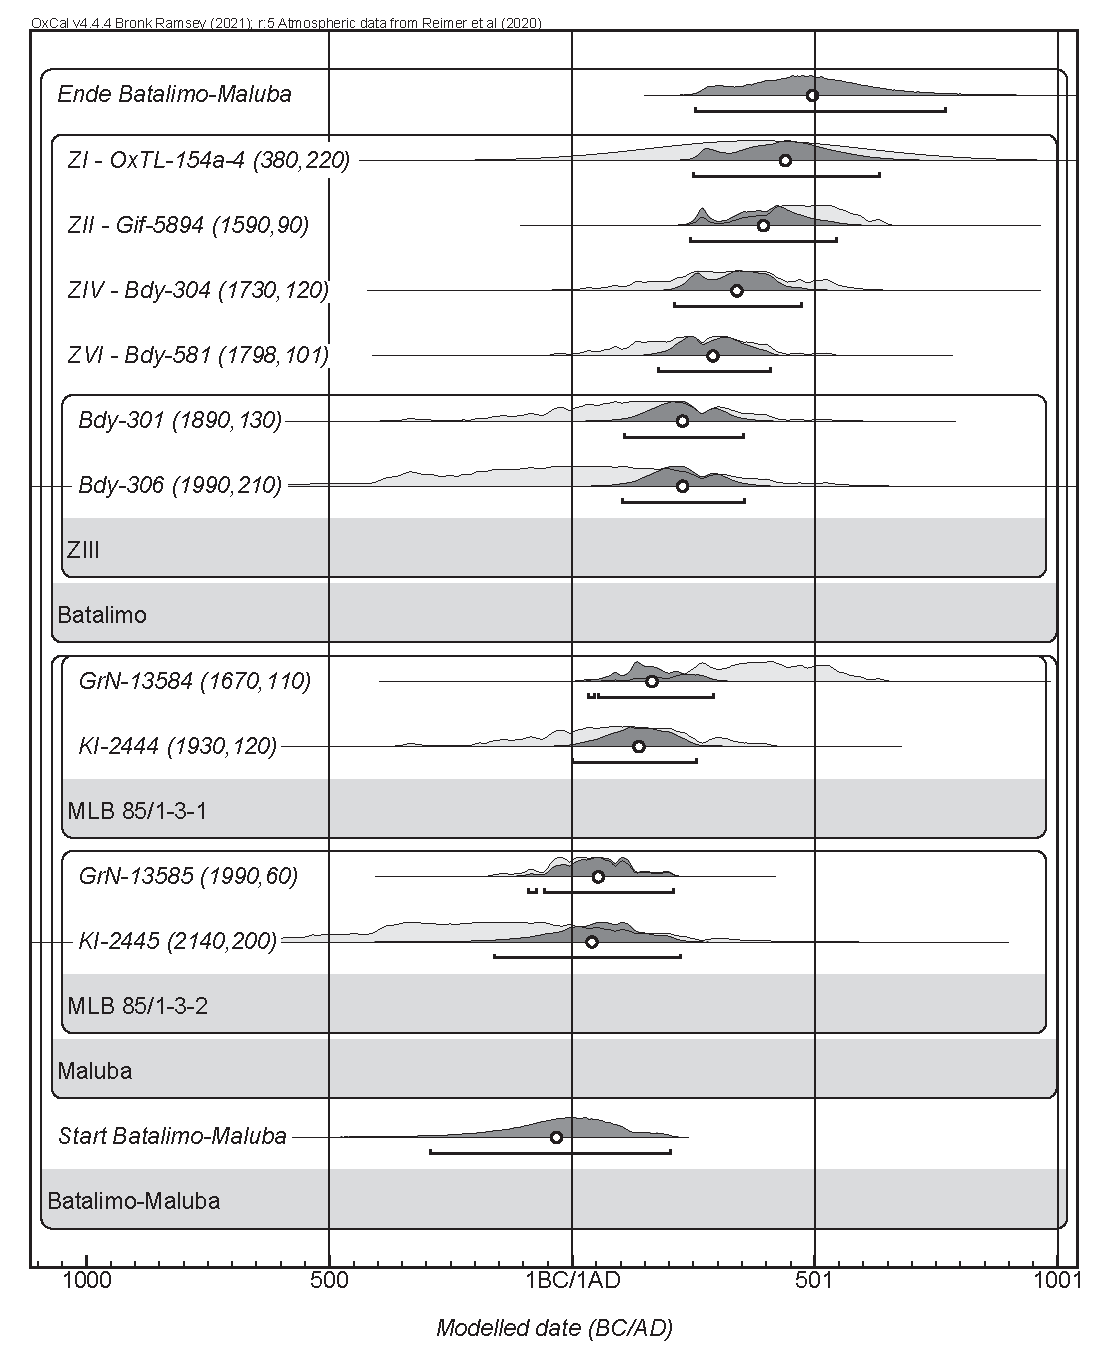
\includegraphics[width=\columnwidth]{fig/BTM_14C.pdf}
	\end{minipage}\hfill
	\noindent\begin{minipage}[b]{\columnwidth}
		\captionof{figure}{Batalimo-Maluba-Gruppe: Kalibierung der \textsuperscript{14}C-Datierungen aus Batalimo am Lobaye und Maluba am Lua (Fpl.~230) \parencites[233]{Aumassip.1975}{deMaret.1985b}{Eggert.1987c}{Kote.1992}{Eggert.1993}{Zangato.2000}.\label{fig:BTM14C}}
	\end{minipage}
\end{figure*}

\begin{figure*}[p]
	\centering
	\includegraphics[width=\textwidth]{fig/BTM_Verbreitung.pdf}
	\caption{Batalimo-Maluba-Gruppe: Verbreitung \parencites[grau; nach][206]{deBayledesHermens.1975}[41\,f. Abb.~4]{Kote.1992}.}
	\label{fig:BTM-Verbreitung}
\end{figure*}

\paragraph{Verzierungen}\hspace{-.5em}|\hspace{.5em}%
Die Keramik der Batalimo-Maluba-Gruppe ist regelhaft verziert. Lediglich etwa 7\,\% aller GE weisen keine Verzierung auf. Im Mittel fanden sich an den GE drei unterschiedliche Verzierungselemente. Mit Blick auf die Verzierungszonen fällt auf, dass die Unterteile und Böden der Batalimo-Maluba-Keramik bis auf äußerst wenige Ausnahmen unverziert sind (Anlage~4.1). Auch die Außenseite der Ränder sind grundsätzlich frei von Verzierungen. Auf den Innenseiten finden sich hingegen regelhaft mit dem Randabschluss parallel verlaufende Rillenbündel (Tab.~\ref{tab:Verzierungselemente}: 02.1). Überdies wurden Verzierungen auf den Hals- und Schulterbereichen sowie dem Bauch der Gefäße aufgebracht. Lediglich knapp 7\,\% aller GE zeigen Verzierungen außerhalb dieser Zierzonen. Das mit Abstand häufigste Verzierungselement bilden horizontale Rillen (Tab.~\ref{tab:Verzierungselemente}: 02.1; 42\,\%). Ebenfalls lassen sich aus überkreuzenden Rillen gebildete \textit{Schachbrett}-Muster (Tab.~\ref{tab:Verzierungselemente}: 01.2; 7\,\%) und Rillen in Zickzack-Mustern (Tab.~\ref{tab:Verzierungselemente}: 01.6; 4\,\%), sowie diagonale (Tab.~\ref{tab:Verzierungselemente}: 02.3; 5\,\%) und gebogene Rillenbündel (Tab.~\ref{tab:Verzierungselemente}: 02.5; 4\,\%), häufig in Kombination miteinander, beobachten. Auffällig ist auch die Unterteilung von Gruppen von Verzierungselementen durch vertikale Rillen (Tab.~\ref{tab:Verzierungselemente}: 02.2; 4\,\%), was zu einer metopenartigen Strukturierung der verzierten Gefäßoberfläche führt. Des Weiteren zeigen die GE auch horizontale Bänder mit runden beziehungsweise leicht ovalen (Tab.~\ref{tab:Verzierungselemente}: 04.11; 4\,\%) oder diagonal gesetzten, kantigen Eindrücken (Tab.~\ref{tab:Verzierungselemente}: 04.12; 4\,\%). Diagonaler Kammeindruck lässt sich ebenfalls beobachten (Tab.~\ref{tab:Verzierungselemente}: 05.1; 4\,\%). Aufgrund des hohen Anteils an miteinander kombinierten Verzierungselementen hat keiner der vertreten Typen, mit Ausnahme der horizontalen Rillen, einen deutlichen Anteil. Zwar insgesamt seltener, aber ebenfalls für die Keramik der Batalimo-Maluba-Gruppe charakteristisch sind kleine, winkelige (Tab.~\ref{tab:Verzierungselemente}: 04.6; 3\,\%) oder Kreisaugen-Eindrücke (Tab.~\ref{tab:Verzierungselemente}: 04.7; 2\,\%). 

\paragraph{Datierung}\hspace{-.5em}|\hspace{.5em}%
Aus beiden 1985 in Maluba am Lua ausgegrabenen Gruben, die Keramik der Batalimo-Maluba-Gruppe enthielten (Kat.-Nr. 1--2), stammen jeweils zwei Radiokohlenstoffdatierungen. Während eine Datierung (KI-2445) eine sehr große Standardabweichung aufweist, ergeben alle Proben jedoch grundsätzlich einen konsistenten Datierungsansatz für die Stilgruppe. Ohne die weite Spanne des Datums KI-2445 weisen die Datierungen auf einen Zeitansatz vom 2. Jh.~v.~Chr bis in das 6. Jh. n.~Chr. (Abb.~\ref{fig:BTM14C}).

Eine Scherbe aus der 1968 in Batalimo am Lobaye erfassten \textit{Kulturschicht} -- Z\,I nach \textcite[117\,f. Tab.~10]{Kote.1992} -- wurde mittels Thermolumineszenzdatierung in das 1. Jh.~v.~Chr bis in das 10. Jh. n.~Chr. datiert \parencite[233; OxTL-154a-4]{Aumassip.1975}. Eine in das 3. Jh. v.~Chr. bis 7. Jh. n.~Chr. datierende Radiokohlenstoffprobe stammt aus der Sondage von Vidal (Bereich Z\,II nach \textsc{Koté} 1992: 117\,f. Tab.~10). Die Grabungen von \textsc{Koté} (ebd. 117\,f. Tab.~10) lieferten sechs weitere Radiokohlenstoffdatierungen für den Fundplatz Batalimo. Eine Probe aus Grabungsschnitt Z\,IV, der an die 1981 durch Vidal angelegten Sondage anschließt, datiert in das 1.--6.~Jh.~n.~Chr. (Bdy-304). Zwei Datierungen aus der in Schnitt Z\,III erfassten Grube decken aufgrund hoher Standardabweichungen einen Zeitraum vom 6. Jh. v.~Chr. bis in das 6. Jh. n.~Chr. ab \parencite[Bdy-301, Bdy-306;][120]{Kote.1992}. Die drei Radiokohlenstoffdatierungen aus der Grube in Schnitt Z\,VI liegen deutlich auseinander. Während eine Datierung aus dem oberen Bereich der Grube in das 6.--11.~Jh. n.~Chr. fällt (Bdy-465), datiert eine Probe von der Grubensohle in das 15.--20.~Jh. n.~Chr. (Bdy-462; ebd. 121). Worin die Ursache dieses auffällig jungen Alters liegen, kann basierend auf dem vorliegenden Bericht von \textsc{Koté} (ebd.) nicht mehr nachvollzogen werden. Eine Schneckenschale von der Sohle derselben Grube lieferte eine Datierungsspanne vom 1. Jh. v.~Chr. bis 5.~Jh. n.~Chr. (Bdy-581; ebd. 121). Ohne genaue Kenntnis und Zuordnung von Befunden, Funden und Datierungsproben, kann die in Schnitt Z\,VI erfasste Grube folglich nur unter starken Vorbehalten und lediglich mit Blick auf die Radiokohlenstoffdatierung Bdy-581 der Batalimo-Maluba-Gruppe zugerechnet werden.\footnote{Während sich dieses letzte Datum mit den aus Maluba stammenden Datierungsansätzen für Keramik der Batalimo-Maluba-Gruppe in Einklang bringen lässt, muss für die zweitälteste Datierung aus dem Befund schon die aus der ersten Grabung im Jahr 1967 stammende Thermolumineszenzdatierung (OxTL-154a-4), herangezogen werden. Zwischen dieser und der Datierung Bdy-465 ergibt sich eine Überlappung der auf 2-Sigma kalibrierten Alterspanne (Abb.~\ref{fig:BTM14C}). Das jüngste Datum liegt vollkommen außerhalb der bekannten Datierungsspanne. Siehe Anm.~\ref{ftn:Kote1992ZuordnungProblem}.}

Insgesamt stehen für die Batalimo-Maluba-Gruppe fünf sicher mit entsprechender Keramik assoziierte Datierungen zur Verfügung (Abb.~\ref{fig:BTM14C}: OxTL-154a-4, KI-2444, KI-2445, GrN-13584 und GrN-13585). Des Weiteren fallen fünf Radiokohlenstoffdatierungen aus den Grabungen von Vidal und \textcite{Kote.1992} in Batalimo in die Zeitspanne, die ohne Vorbehalte mit Batalimo-Maluba-Keramik in Zusammenhang steht (Abb.~\ref{fig:BTM14C}: Bdy-301, Bdy-306, Bdy-304 und Bdy-581 sowie Gif-5894). Da jedoch unklar ist, wie das zusammen mit diesen Proben angetroffene Fundgut aussieht, können diese nicht zweifelsfrei der Batalimo-Maluba-Gruppe zugerechnet werden. Auch handelt es sich bei allen Datierungen um konventionelle Messungen, die zudem häufig sehr hohe Standardabweichungen aufweisen. Zusammenfassend kann anhand der gegenwärtig vorliegenden Daten nur das 2. Jh. v.~Chr. bis 6. Jh. n.~Chr. als Zeitansatz für die Batalimo-Maluba-Keramik gelten (Abb.~\ref{fig:BTM14C}).

\paragraph{Verbreitung}\hspace{-.5em}|\hspace{.5em}%
Keramik  des Batalimo-Maluba-Stils findet sich in einem deutlich abgegrenzten Raum entlang dem Oberlauf des \mbox{Ubangi} sowie im Bereich der Mündung des Lua (Abb.~\ref{fig:BTM-Verbreitung}). Die nördliche Grenze der Verbreitung liegt etwas stromauf des \mbox{Ubangi}-Bogens bei Mokelo (Fpl.~213).\footnote{Auffällig ist die Nähe des Verbreitungsgebietes der Batalimo-Maluba-Keramik zur rezenten Nordgrenze des äquatorialen Regenwaldes (Abb.~\ref{fig:BTM-Verbreitung}). Nimmt man jedoch die von \textcite[7 Abb.~4]{Maley.2001} postulierte Grenze der Verbreitung des Regenwaldes im 1.~Jt. v.~Chr. als Grundlage, so liegt das Gros der Fundstellen außerhalb des Waldes. Erst zukünftige Untersuchungen zur Paläo-Umwelt dieses Raumes werden jedoch in der Lage sein, das ökologische Umfeld zur Zeit des Batalimo-Maluba-Stils zu ergründen (siehe Kap.~\ref{sec:Palaeoumwelt}).} Im Süden reicht die Hauptverbreitung bis in den Bereich südlich der Mündung des Lua. Vereinzelte Stücke finden sich auch weiter südlich, so zum Beispiel in Ebeka (Fpl.~197) und \mbox{Ngbanja} (Fpl.~199). Entlang des Lua fand sich lediglich in Maluba (Fpl.~230) Keramik des Batalimo-Maluba-Stils.\footnote{Zusammengenommen lagen von den drei ebenfalls am Lua gelegenen Fundplätzen Imboto (Fpl.~231), Ilawa (Fpl.~232) und Fulu-Kaba (Fpl.~233) lediglich 22 GE vor, die aufgrund starker Fragmentierung nur in fünf Fällen einer keramischen Stilgruppe zugerechnet werden konnten. Dabei handelte es sich ausschließlich um Vertreter der jüngeren Stilgruppen Dongo (Kap.~\ref{sec:DON-Gr}), Motenge-Boma (Fpl.~\ref{sec:MTB-Gr}) und Dama (Kap.~\ref{sec:DAM-Gr}).} Das am unteren Lobaye gelegene Batalimo \parencite{deBayledesHermens.1975} liegt in der nördlichen Hälfte des Verbreitungsgebietes.

Zusätzlich zu Batalimo am Lobaye \parencite{deBayledesHermens.1975} sowie den durch das \textit{River Reconnaissance Project} erschlossenen, hier vorgestellten Fundstellen, wird Keramik der Batalimo-Maluba-Gruppe noch von zwei weiteren Fundplätzen berichtet: In Ngo Tchoro, das 1,5\,km nördlich von Batalimo wohl ebenfalls nahe des Lobaye liegt, erbrachte ein 2009 angelegter Testschnitt Keramik, die jener der Batalimo-Maluba-Gruppe entsprechen soll \parencite{Ndanga.2010}. Von der am \mbox{Ubangi} gelegenen, aber nicht näher lokalisierbaren Fundstelle Mongo~II wird eine Grube mit geschliffenen Beilen, Batalimo-Maluba-Keramik sowie Belegen für Eisenverarbeitung berichtet \parencite{Ndanga.20120623}.\footnote{Gegenwärtig ist keines der beiden keramischen Inventare aufgearbeitet und veröffentlicht.}

\begin{figure*}[tb]
	\centering
	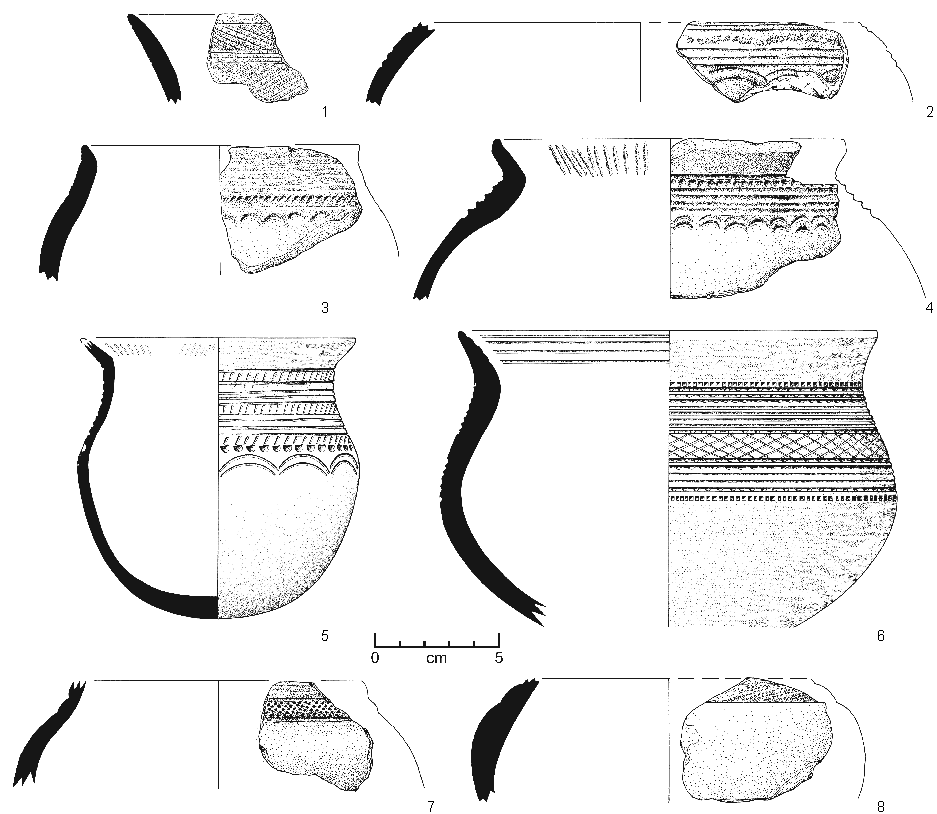
\includegraphics[width=.925\textwidth]{fig/NGB-Typen.pdf}
	\caption{\mbox{Ngbanja}-Gruppe: Typvertreter.\\1:~Taf.~58.14; 2:~Taf.~60.14; 3:~Taf.~6.10; 4:~Taf.~6.6; 5:~6.8; 6:~Taf.~6.7; 7:~Taf.~47.20; 8:~Taf.~6.9.}
	\label{fig:NGB_Typverteter}
\end{figure*}

\subsubsection{\mbox{Ngbanja}-Gruppe}\label{sec:NGB-Gr}

Eine deutliche Ähnlichkeiten zur Batalimo-Maluba-Keramik (siehe Kap.~\ref{sec:BTM-Gr}) aufweisende, sich von dieser jedoch auch deutlich unterscheidende Keramik findet sich vor allem entlang des mittleren und unteren \mbox{Ubangi}. Funde der, nach der Fundstelle \mbox{Ngbanja} (Fpl.~199) am mittleren \mbox{Ubangi} benannten Stilgruppe sind bislang fast ausschließlich aus Oberflächenabsammlungen bekannt. Die aus Grabungen bekannten Stücke machen zusammen 10\,\% aller der \mbox{Ngbanja}-Gruppe zugewiesenen GE aus.\footnote{1985 wurden bei den Grabungen in Maluba am Lua (Fpl.~230) zwei GE erfasst, deren Zuweisung zur \mbox{Ngbanja}-Gruppe jedoch fraglich ist. Bei den Grabungen in Pikunda am mittleren \mbox{Sangha} (Fpl.~255) wurden 1987 vier weitere GE ausgegraben. Eine sichere Einordnung dieser Stücke in die \mbox{Ngbanja}-Gruppe ist jedoch ebenfalls fraglich.} In den entsprechenden Inventaren bilden diese aber in jedem Fall isolierte Einzelfunde. Ein Befund, in dem die \mbox{Ngbanja}-Keramik dominiert, wurde bislang nicht erfasst. Neben der chronologischen Stellung lässt sich daher auch das formale Spektrum der Stilgruppe nur bedingt beschreiben. Folglich kann die \mbox{Ngbanja}-Gruppe beim gegenwärtigen Quellenstand lediglich als Provisorium angesehen werden.\footnote{Siehe auch \textcite[185\,f., 202]{Wotzka.1995} zur Zuweisung von nur spärlich in den im untersuchten Inventar belegten, aber charakteristischen keramischen Formen zu \enquote{Stilgruppen} mit provisorischem Charakter.\label{ftn:ProvisorischeStilGr}}

Insgesamt liegen 60~GE vor, die der \mbox{Ngbanja}-Gruppe zugewiesen wurden, wobei lediglich 20~GE als sicher der Stilgruppe zugehörig angesprochen wurden. Die zweifelsfrei der \mbox{Ngbanja}-Gruppe zugewiesenen Stücke stammen von lediglich sechs Fundstellen entlang des mittleren \mbox{Ubangi} sowie oberen \mbox{Sangha} (Abb.~\ref{fig:NGB_Verbreitung}): \mbox{Ngbanja} (Fpl.~199), Nzambi (Fpl.~205), Pikunda (Fpl.~255), Matoto (Fpl.~264), Ouesso (Fpl.~265) und Pandama (Fpl.~276). Bereits \textcite[140\,f. Fig.~13.4--5]{Eggert.1987c} war sich über die genaue Zuordnung der im Rahmen dieser Arbeit unter der Bezeichnung \mbox{Ngbanja} subsumierten Keramik nicht sicher. Einerseits sah er klare Ähnlichkeiten zur Keramik von Batalimo und Maluba, andererseits jedoch auch ebenso deutliche Unterschiede zu dieser.\footnote{Siehe Anm.~\ref{ftn:BTM-NGB-Unterschiede}.} Die fraglichen Formen konnten aufgrund der seit 1987 unveränderten Datenlage auch in der vorliegenden Auswertung nicht abschließend klassifiziert werden. Hier können, wie bereits auch von \textsc{Eggert} (ebd. 141) festgestellt, nur neue Grabungen eine Abhilfe schaffen.

\paragraph{Technologische Merkmale}\hspace{-.5em}|\hspace{.5em}%
Die Keramik der \mbox{Ngbanja}-Gruppe weist eine auffällige technologische Vielfalt auf. Das Material wird von Vertretern der \textit{Fabrics} 4a (23\,\%) und 4c (19\,\%) bestimmt, die zusammen knapp die Hälfte aller Funde abdecken. Ebenfalls häufig kommen die \textit{Fabrics} 5c (12\,\%) sowie 5b (8\,\%) vor. Wie auch bei der Keramik der Batalimo-Maluba-Gruppe (Kap.~\ref{sec:BTM-Gr}) dominieren die an mineralischen nichtplastischen Partikeln reichen und aus rotbrennenden Tonen gefertigten \textit{Fabrics} 4 und 5. Dies bedeutet, dass die GE viel bis sehr viel nichtplastisches Material (ca.~80\,\%) enthalten, das sich vor allem aus heterogenen Mischungen von Quarzsanden (>~80\,\%) zusammensetzt. In einigen Fällen ließen sich auch Laterit sowie Glimmer oder ausgebrannte Organik in den Scherben beobachten. Die Oberflächen der 20~GE, die sicher der \mbox{Ngbanja}-Gruppe zugewiesen wurden, schwankt zwischen rau und gut geglättet. An einigen Fundstellen, so an der namensgebenden Fundstelle \mbox{Ngbanja} (Fpl.~199), sind die Oberflächen eher gut geglättet, während sie in Nzambi (Fpl.~205) eher rau sind. Die mittlere Wandungsdicke der Scherben der \mbox{Ngbanja}-Gruppe liegt bei 7,3\,mm, bei einer Varianz von 2,9\,mm. Präferenzen bei der Auswahl der genutzten Tone bezüglich ihrer Brennfarbe ließen sich nicht erkennen. Während Scherben aus eindeutig rotbrennenden Tonen einen großen Anteil einnehmen (38\,\%) sind auch Stücke aus weißbrennenden Tonen in nicht unerheblichen Maße vertreten (23\,\%).


\paragraph{Formen}\hspace{-.5em}|\hspace{.5em}%
Insgesamt konnte lediglich bei acht von 26~GE, bei denen eine Ansprache der Gefäßform grundsätzlich möglich war, die Gefäßform auch sicher bestimmt werden. Das Formenspektrum wird von leicht bauchigen Gefäßen mit schwach ausgeprägter Schulterpartie bestimmt (Typ~C1; Abb.~\ref{fig:NGB_Typverteter}.2--3,5--8). Insgesamt sind 13~GE des Typs C1 bekannt, diese machen zusammengenommen mehr als 60\,\% aller mit einer Gefäßform angesprochenen GE aus. Bauchige Gefäße mit einem deutlich herausgearbeiteten Schulterbereich (Typ C2), die für die Batalimo-Maluba-Gruppe so charakteristisch sind, fanden sich im Material der \mbox{Ngbanja}-Gruppe lediglich ein Mal. Es konnten auch nur sehr wenige offene Gefäßformen beobachtet werden. Unter den 27~GE, bei denen eine Randform angesprochen werden konnte, entfällt mehr als die Hälfte auf einfache (B1) oder leicht konkav ausbiegende Ränder (B2). Die Ränder weisen in der Regel eine spitz zulaufende (M2; 27\,\%) oder gerillte Randlippe (M4; 20\,\%) auf. Lediglich bei einer, sicher der \mbox{Ngbanja}-Gruppe zuweisbaren GE konnte ein runder Boden (B1) beobachtet werden (Abb.~\ref{fig:NGB_Typverteter}.5). Bei zwei GE, die jedoch nicht zweifelsfrei der \mbox{Ngbanja}-Gruppe angehören müssen, wurden hingegen flache Standböden vom Typ B4 festgestellt. Auf dieser Basis kann keine Aussage getroffen werden, ob die \mbox{Ngbanja}-Keramik, wie die Batalimo-Maluba-Keramik, grundsätzlich als flachbodig bezeichnet werden kann.


\paragraph{Verzierungen}\hspace{-.5em}|\hspace{.5em}%
Das bestimmende Verzierungselement der \mbox{Ngbanja}-Gruppe sind horizontale Rillen (Tab.~\ref{tab:Verzierungselemente}: 02.1), die 45\,\% aller beobachteten Verzierungen ausmachen. Diese fanden sich bis auf die Gefäßunterteile und Böden an allen Gefäßpositionen in gleichem Maße (Anlage~4\subref{fig:NGB_Verz}). Auffällig sind das regelmäßige Auftreten innenseitig gerillter Ränder, ein Merkmal, das die \mbox{Ngbanja}-Keramik mit der Batalimo-Maluba-Keramik teilt. Anders als diese, weisen aber auch die Außenseiten der Ränder häufig Verzierungen auf. Diagonale Schachbrettmuster (Tab.~\ref{tab:Verzierungselemente}: 01.2) bilden mit 9\,\% aller Verzierungselemente die zweithäufigste Verzierung und sind regelhaft am Rand (Abb.~\ref{fig:NGB_Typverteter}.1) sowie den Schulterbereichen der Gefäße zu finden (Abb.~\ref{fig:NGB_Typverteter}.6). Kammeindrücke (Tab.~\ref{tab:Verzierungselemente}: 05.1; 7\,\%) sowie horizontale Reihen aus bogenförmigen Eindrücken (Tab.~\ref{tab:Verzierungselemente}: 04.19; 6\,\%) können ebenfalls beobachtet werden. Letztere lassen sich vornehmlich unterhalb der Rillenzier auf der Schulter- beziehungsweise Bauchpartie der Gefäße als untere Abschluss der Verzierungszone finden (Abb.~\ref{fig:NGB_Typverteter}.2, 4--5, Taf.~6.10). Horizontale Reihen aus Eindrücken (4.12) sind bei einigen GE zu beobachten (Abb.~\ref{fig:NGB_Typverteter}.6). Zwei GE zeichnen sich durch eine flache horizontale Leiste (Tab.~\ref{tab:Verzierungselemente}: 09.2) mit Kammeindrücken (Tab.~\ref{tab:Verzierungselemente}: 05.1) aus (siehe Abb.~\ref{fig:NGB_Typverteter}.7--8). Es handelte sich um die einzige Verzierung der entsprechenden GE.\footnote{Die auffällige Ähnlichkeit der beiden Stücke stellt einen vagen Bezug zwischen den beiden Fundstellen \mbox{Ngbanja} am mittleren \mbox{Ubangi} (Fpl.~199; Abb.~\ref{fig:NGB_Typverteter}.8) und Pikunda am mittleren \mbox{Sangha} (Fpl.~250; Abb.~\ref{fig:NGB_Typverteter}.7) her. Da keine eindeutige Vergesellschaftung dieser beiden Stücke mit anderen Formen des \mbox{Ngbanja}-Stils belegt ist, muss ihre Zuweisung jedoch fraglich bleiben. In \mbox{Ngbanja} selbst konnte aufgrund starker Fragmentierung der Surveyfunde mehr als die Hälfte aller GE keiner Stilgruppe zugewiesen werden. Unter den Stücken, die stilistisch angesprochen werden konnten, macht das Material der \mbox{Ngbanja}-Gruppe den größten Anteil aus.} An Gefäßunterteilen, Bodenansätzen und Standflächen konnte bei keiner der der \mbox{Ngbanja}-Gruppe zugewiesenen GE eine Verzierung beobachtete werden. 


\paragraph{Datierung}\hspace{-.5em}|\hspace{.5em}%
Das unter der Bezeichnung \mbox{Ngbanja} subsumierte keramische Fundgut stammt fast ausschließlich von Oberflächensurveys und Angaben zur Datierung der Stilgruppe können lediglich indirekt erfolgen. Einzig in der älteren Grube B1/B2 in PIK~87/1 (Kat.-Nr.~8) in Pikunda am \mbox{Sangha} fanden sich neben der für den Befund charakteristischen Pikunda-Munda-Keramik (Kap.~\ref{sec:PKM-Gr}) einige wenige, möglicherweise der \mbox{Ngbanja}-Gruppe zuweisbare Scherben (Tab.~\ref{tab:PIK87-1bis9_nichtPIK-MUN}). Diese können als Datierungsindiz gewertet werden, sind aber aufgrund mangelnder Sicherheit in der Bestimmung nur ein sehr schwacher Anhaltspunkt. Die drei GE sind mit Keramik der Pikunda-Munda-Gruppe sowie einer Scherbe der Lusako-Gruppe \parencite[Kap.~\ref{sec:LUS-Gr};][104--107]{Wotzka.1995} vergesellschaftet und werden durch eine Radiokohlenstoffdatierung zwischen das 4.~Jh. v.~Chr. und 3.--4.~Jh. n.~Chr. datiert (Tab.~\ref{tab:PIK87-1_Datierungen}: KI-2877).

\begin{figure*}[p]
	\centering
	\includegraphics[width=\textwidth]{fig/NGB_Verbreitung.pdf}
	\caption{\mbox{Ngbanja}-Gruppe: Verbreitung.}
	\label{fig:NGB_Verbreitung}
\end{figure*}

Da die Keramik der \mbox{Ngbanja}-Gruppe in keiner Grabung hinreichend nachgewiesen werden konnte, beruhen Angaben zur chronologischen Stellung der Keramik fast ausnahmslos auf losen, sich aus Vergleichen auf Merkmalsebene ergebenden Indizien. Mit Blick auf die formalen Charakteristika der \mbox{Ngbanja}-Keramik fallen deutliche Ähnlichkeiten zur Batalimo-Maluba-Gruppe auf (Kap.~\ref{sec:BTM-Gr}). \textcite[140\,f.]{Eggert.1987c} weist auf deutliche Unterschiede eines Gefäßes aus Ebeka (Taf.~5.7)\footnote{Das von \textsc{Eggert} (1987b: 140\,f., 142 Abb.~12.1; Taf.~5.7) aufgeführte Gefäß aus Ebeka wurde in der vorliegenden Analyse weder sicher der \mbox{Ngbanja}- noch der Batalimo-Maluba-Gruppe zugerechnet. Die Grundform des Gefäßes (siehe Abb.~\ref{Fig-BatMLB-Typvertreter}.6) sowie die die Verzierung bildenden Muster, vornehmlich das auffällige Zickzack-Band auf dem Gefäßbauch (siehe Abb.~\ref{Fig-BatMLB-Typvertreter}.5), weisen auf eine Nähe zur Batalimo-Maluba-Keramik hin. Ähnliche Gefäßformen sind aber auch aus der \mbox{Ngbanja}-Gruppe belegt (Abb.~\ref{fig:NGB_Typverteter}.4). Gerade die mangelnde Sorgfalt, mit der die Verzierungen auf dem Gefäß aus Ebeka aufgebracht sind, grenzt es jedoch vom Batalimo-Maluba-Stil ab, dessen Gefäße sich durch technisch äußerst sorgfältige und fein gearbeitete Verzierungen auszeichnen. Auch die Verzierung der Innenseite des Randes mit einem feinen diagonalen Schachbrett ließ sich bei keiner GE der Batalimo-Maluba-Gruppe beobachten. Das gleiche gilt für die breiten Rillen auf dem Gefäßhals. Entsprechende Parallelen finden sich jedoch in Formen der \mbox{Ngbanja}-Gruppe (Abb.~\ref{fig:NGB_Typverteter}.3). Diese Mischung aus Charakteristika verhinderte eine sichere Zuweisung des Gefäßes zu einer der beiden Stilgruppen.\label{ftn:BTM-NGB-Unterschiede}} sowie der Gefäße aus \mbox{Ngbanja} (Abb.~\ref{fig:NGB_Typverteter}.5--6) zur jüngeren Keramik entlang des mittleren \mbox{Ubangi} hin. Zur älteren Batalimo-Maluba-Keramik grenzen sich die angeführten Stücke vor allem durch den am Gefäß aus \mbox{Ngbanja} zu beobachtenden runden Boden ab (Abb.~\ref{fig:NGB_Typverteter}.5). \textsc{Eggert} (ebd. 141) hebt jedoch zugleich hervor, dass auch die flachen Böden der Batalimo-Maluba-Gruppe teilweise nur wenig abgesetzt sind und daher einen abgerundeten Eindruck vermitteln können. Mit der Batalimo-Maluba-Gruppe hat die \mbox{Ngbanja}-Keramik die Nutzung diagonaler Schachbrettmuster gemein (Tab.~\ref{tab:Verzierungselemente}: 01.2), die bei der \mbox{Ngbanja}-Gruppe jedoch deutlich grober ausgeführt sind. Die innen gerillten Ränder der \mbox{Ngbanja}-Keramik finden sich auch im Fundgut der Stilgruppen Batalimo-Maluba (Kap.~\ref{sec:BTM-Gr}) sowie Dongo (Kap.~\ref{sec:DON-Gr}). Gemeinsam mit der Dongo-Keramik hat die \mbox{Ngbanja}-Keramik rillenverzierte Gefäßhälse sowie girlandenartig umlaufende, bogenförmige Rillen (siehe Abb.~\ref{fig:DON_Typverteter}.8), grenzt sich von dieser aber auch durch die deutlich unterschiedliche Randgestaltung ab.

Zusammenfassend kann festgehalten werden, dass die \mbox{Ngbanja}-Gruppe eine ritzverzierte, eher grobe Keramik beschreibt, die stilistische Ähnlichkeiten zur ältesten Stilgruppe entlang des \mbox{Ubangi}-Gebietes, der Batalimo-Maluba-Gruppe, aufweist und unter Hinzuziehung einer Radiokohlenstoffdatierung aus Pikunda am Sangha (KI-2877) vorläufig in das 4.~Jh. v.~Chr. bis 3.--4.~Jh. n.~Chr. datiert werden kann. Dass die hauptsächlich mit Keramik der Pikunda-Munda-Gruppe (Kap.~\ref{sec:PKM-Gr}) assoziierte Radiokohlenstoffdatierung aus Pikunda für den vor allem am unteren Ubangi belegten \mbox{Ngbanja}-Stil als repräsentativ angesehen werden kann, gründet auf zwei nahezu identischen Scherben aus Ngbanja und Pikunda (Abb.~\ref{fig:NGB_Typverteter}.7--8). Vergleichbare Stücke fanden sich an keinem anderen Fundplatz im gesamten Arbeitsgebiet. Die unter der Bezeichnung \mbox{Ngbanja} subsumierte Keramik kann -- unter Vorbehalt -- als Phänomen der frühen Eisenzeit im Arbeitsgebiet und zumindest als teilweise zeitgleich zu den Stilgruppen Batalimo-Maluba (Kap.~\ref{sec:BTM-Gr}) wie Pikunda-Munda (Kap.~\ref{sec:PKM-Gr}) angesehen werden.

\paragraph{Verbreitung}\hspace{-.5em}|\hspace{.5em}%
Keramik, die der \mbox{Ngbanja}-Gruppe zugewiesen wurde, fand sich an 13 Fundplätzen, vornehmlich im Zentrum des Arbeitsgebietes (Abb.~\ref{fig:NGB_Verbreitung}). Sicher der \mbox{Ngbanja}-Gruppe zugewiesene Stücke fanden sich an lediglich sechs dieser 13 Plätze. Entlang des mittleren \mbox{Ubangi} sind dies der eponyme Fundplatz \mbox{Ngbanja} (Fpl.~199) und Nzambi (Fpl.~205), während Nbganja-Keramik weiter westlich, am mittleren bis oberen \mbox{Sangha} aus Pikunda (Fpl.~255), Matoto (Fpl.~264), Ouesso (Fpl.~265) sowie Pandama (Fpl.~276) bekannt ist. Mehr als ein Vertreter der \mbox{Ngbanja}-Gruppe fand sich lediglich in \mbox{Ngbanja} und Nzambi am mittleren \mbox{Ubangi} sowie Ouesso und Ikelemba (Fpl.~260) am mittleren \mbox{Sangha}; letztere Funde sind jedoch lediglich unter Vorbehalt der Stilgruppe zuzuweisen. Das Verbreitungsgebiet der \mbox{Ngbanja}-Gruppe ist insofern außergewöhnlich, da sich dieser Stilgruppe zugeordnete Keramik jeweils an den mittleren Flussläufen des \mbox{Ubangi} und \mbox{Sangha} findet, nicht jedoch im Mündungsgebiet der beiden Flüsse (Abb.~\ref{fig:NGB_Verbreitung}). Die Gebiete sind folglich nicht über die Flüsse miteinander verbunden. Dieses Verbreitungsbild gibt Grund zur Vorsicht und zukünftige Feldforschung muss zeigen, ob sich die Zuweisung der hier subsumierten Formen zu einer Stilgrupppe aufrecht erhalten lässt.

Akzeptiert man die \mbox{Ngbanja}-Gruppe und ihr Verbreitungsgebiet, so fällt auf, dass sie sich etwas weiter südlich als die Keramik der Batalimo-Maluba-Gruppe (Abb.~\ref{fig:BTM-Verbreitung}) findet, jener Stilgruppe, der die bislang ältesten, hinreichend belegten Spuren keramischer Erzeugnisse im \mbox{Ubangi}- und Lua-Gebiet zuzuordnen sind. Die chronologische Ansprache der \mbox{Ngbanja}-Keramik deutet auf eine hypothetische Gleichzeitigkeit dieser beiden Stilgruppen sowie der Pikunda-Munda-Gruppe des \mbox{Sangha}- und Likwala-aux-Herbes-Gebiets hin. Mit Bezug auf die Pikunda-Munda-Gruppe (Abb.~\ref{fig:PIKMUN_Verbreitung}) fällt auf, dass sich die Funde des \mbox{Ngbanja}-Stils entlang des \mbox{Sangha} eher stromauf finden. Zieht man die Kartierung der Regenwaldrefugien nach \textcite[7 Abb.~4]{Maley.2001} hinzu, so lässt sich erkennen, dass die Batalimo-Maluba-Gruppe im Norden außerhalb des postulierten Refugiums zu finden ist, während die Pikunda-Munda-Keramik im westlichen Teil des Refugiums verortet werden müsste. Die Fundpunkte der \mbox{Ngbanja}-Gruppe zeichnen hingegen den nordöstlichen Rand des Regenwald-Refugiums im Kongobecken nach. 

\begin{figure*}[tb]
	\centering
	\includegraphics[width=\textwidth]{fig/DON-Typen.pdf}
	\caption{Dongo-Gruppe: Typvertreter.\\1:~Taf.~9.7; 2:~Taf.~8.6; 3:~Taf.~9.8; 4:~Taf.~11.4; 5:~Taf.~7.13; 6:~Taf.~11.3; 7:~Taf.~10.6; 8:~Taf.~8.1; 9:~Taf.~7.14; 10:~Taf.~8.3; 11:~Taf.~10.3.}
	\label{fig:DON_Typverteter}
\end{figure*}

\subsubsection{Dongo-Gruppe}\label{sec:DON-Gr}

Die Dongo-Gruppe beschreibt eine ritzverzierte Keramik, die vor allem entlang des mittleren \mbox{Ubangi} verbreitet ist (Abb.~\ref{fig:DON_Verbreitung}). Bis auf eine potenziell zur Dongo-Gruppe gehörende GE aus einem dem Befund MLB~85/1-3-2 (Kat.-Nr.~2) zuweisbaren Komplex von Surveyfunden\footnote{Es handelt sich um den Komplex MLB~85/104, der sich \enquote{unmittelbar rechts neben MLB 85/1} (Kat.-Nr.~1) befunden hat und unter anderem ein Gefäß der Batalimo-Maluba-Gruppe enthielt (Abb.~\ref{Fig-BatMLB-Typvertreter}.5; Feldbuch \textsc{Eggert} 05.09.1985). In diesem Bereich wurde später die Grube MLB~85/1-3-2 (Kat.-Nr.~2) ausgegraben.} an der am unteren Lua gelegenen Fundstelle Maluba (Fpl.~230) stammt alles dieser Stilgruppe zugewiesene Material aus Oberflächenabsammlungen. Die Beschreibung der Stilgruppe basiert auf insgesamt 111~GE, von denen 67~GE zweifelsfrei der Stilgruppe zugewiesen wurden, sowie 37 ausgezählten Stücken. 

\paragraph{Technologische Merkmale}\hspace{-.5em}|\hspace{.5em}%
Die Keramik der Dongo-Gruppe weist eine starke Heterogenität bezüglich der vertretenen \textit{Fabrics} auf. Die Typen 4a (19\,\%) und 4c (14\,\%) sind am häufigsten vertreten. Mit jeweils über 10\,\% ließen sich die Varianten 7d (12\,\%), 3c (11\,\%), 7c (10\,\%) sowie 8a (10\,\%) beobachten. Diese Verteilung der \textit{Fabrics} spiegelt den grundsätzlich mittleren (36\,\%) bis hohen (33\,\%) Anteil nichtplastischer Partikel im Scherben wider. Es handelt sich größtenteils um heterogene Mischungen von Quarzsanden, die in einigen Fällen auch Anteile von Glimmer und seltener auch Laterit enthalten. Die meisten Stücke zeigen eine glatte oder nur leicht raue Oberfläche, die in einigen Fällen auch leicht sandig ist. Die Färbung der Scherben der Dongo-Gruppe weist auf die Nutzung weiß- (33\,\%) wie auch rotbrennender Tone (26\,\%) hin. Das Gros des Materials (41\,\%) zeigt jedoch eine beige, graue sowie schwarze Färbung, wodurch keine zweifelsfreie Ansprache der Brennfarbe der genutzten Tone möglich ist. Dieser Befund unterstreicht die heterogene Natur der technischen Eigenschaften der Dongo-Keramik. Die Wandungsstärke der Dongo-Keramik liegt im Mittel bei 6,8\,mm mit einer Varianz von 2,3\,mm.

\paragraph{Formen}\hspace{-.5em}|\hspace{.5em}%
Bei insgesamt 84~GE, welche der Dongo-Gruppe zugerechnet wurden, konnte die Gefäßform beschrieben werden. Den überwiegenden Teil (58\,\%) machen flache Gefäße mit geschweifter Wandung und ohne ausgearbeiteten Halsbereich aus (Typ~E; Abb.~\ref{fig:DON_Typverteter}.1--4, 6--7), gefolgt von schalenförmigen Gefäßen mit konvexer Wandung (Typ~I; 24\,\%; Abb.~\ref{fig:DON_Typverteter}.8, 10). Weitere Gefäßformen, wie Flaschen (Typ~A; Abb.~\ref{fig:DON_Typverteter}.5) oder schalenförmige Gefäße mit einbiegendem Rand (Typ~H; Abb.~\ref{fig:DON_Typverteter}.9) sind nur vereinzelt vertreten. Aufgrund der Fragmentierung der größtenteils bei Oberflächensurveys gemachten Funde kann in vielen Fällen eine klare Zuweisung nicht erfolgen. Der Bauchbereich der Dongo-Keramik ist regelmäßig konvex ausgeführt (66\,\%; Abb.~\ref{fig:DON_Typverteter}.5, 7). Seltener lassen sich auch stark (7\,\%) sowie schwach konvexe Wandungen (7\,\%; Abb.~\ref{fig:DON_Typverteter}.8--9) beobachten. Die Ränder der Dongo-Gruppe zeigen ebenfalls eine starke Heterogenität. Bei insgesamt 98~GE können zusammen 19 Randformen unterschieden werden. Die häufigste Randform sind sehr kurze ausbiegende Ränder (B1.1, 22\,\%), die ohne eine Halspartie direkt aus dem Schulterbereich der Gefäße hervorgehen. Ebenfalls charakteristisch sind kurz ausbiegende bis gerade Ränder mit einer im Profil dreieckigen Randleiste (A2.3; 18\,\%). Die Halspartie ist häufig überhaupt nicht (29\,\%) oder nur kurz ausgeführt (27\,\%) und der Schulterbereich der Gefäße ist in der Regel konvex (60\,\%; Abb.~\ref{fig:DON_Typverteter}.5, 7). In geringerem Maße kommen auch gerade Schulterpartieren vor (26\,\%; Abb.~\ref{fig:DON_Typverteter}.2, 6). Der Dongo-Gruppe können gegenwärtig lediglich zwei eindeutige Bodenstücke zugerechnet werden. Während eine GE einen flachen Standboden aufweist (B4), ließ sich an der zweiten GE ein Linsenboden beobachten (B2; Abb.~\ref{fig:DON_Typverteter}.10).


\paragraph{Verzierungen}\hspace{-.5em}|\hspace{.5em}%
Die Verzierungspraxis der Dongo-Keramik wird von horizontalen Ritzlinien dominiert (Tab.~\ref{tab:Verzierungselemente}: 02.1; 67\,\%). Diese finden sich regelhaft an der Innenseite der Ränder (Anlage~4\subref{fig:DON_Verz}; \ref{fig:DON_Typverteter}.1--3). Neben horizontalen Rillen ließen sich nur sehr vereinzelt andere Verzierungselemente feststellen. Unter anderem wurde bei zwei GE vegetabilischer \textit{knotted strip}-Roulette (Tab.~\ref{tab:Verzierungselemente}: 21.1) sowie an einer weiteren, potenziell der Dongo-Gruppe zurechenbaren GE Schnitzroulette (Tab.~\ref{tab:Verzierungselemente}: 21.10; Taf.~21.3) beobachtet. In ebenfalls geringen Anteilen ließen sich \textit{Schachbrettmuster} (Tab.~\ref{tab:Verzierungselemente}: 01.3; 5\,\%; Abb.~\ref{fig:DON_Typverteter}.6) und diagonale (Tab.~\ref{tab:Verzierungselemente}: 04.12; 4\,\%) sowie vertikale Eindrücke (Tab.~\ref{tab:Verzierungselemente}: 04.15; 4\,\%; Abb.~\ref{fig:DON_Typverteter}.1, 4, 6, 7, 11)  identifizieren. Die genannten Eindrücke fanden sich fast ausschließlich an der Randlippe (Anlage~4\subref{fig:DON_Verz}).

\begin{figure*}[p]
	\centering
	\includegraphics[width=\textwidth]{fig/DON_Verbreitung.pdf}
	\caption{Dongo-Gruppe: Verbreitung.}
	\label{fig:DON_Verbreitung}
\end{figure*}

\paragraph{Datierung}\hspace{-.5em}|\hspace{.5em}%
Für die Keramik der Dongo-Gruppe liegen keine absoluten Daten vor. Eine chronologische Einordnung der beschriebenen und zu einer Stilgruppe zusammengefassten Formen lässt sich daher nur anhand relativ-chronologischer Indizien, im Vergleich mit anderen Stilgruppen des Arbeitsgebietes erzielen. Eine dieser Ähnlichkeiten ergibt sich zu den Stilen Batalimo-Maluba (Kap.~\ref{sec:BTM-Gr}) und \mbox{Ngbanja} (Kap.~\ref{sec:NGB-Gr}), die wie auch die Dongo-Keramik innenseitig mit feinen Rillenbündeln versehene Ränder aufweisen (Abb.~\ref{Fig-BatMLB-Typvertreter}.5, \ref{fig:NGB_Typverteter}.6). Die umgelegten Ränder der Dongo-Gruppe (Abb.~\ref{fig:DON_Typverteter}.1, 9) zeigen hingegen bedingte Ähnlichkeiten zur Randgestaltung des Motenge-Boma-Stils (Kap.~\ref{sec:MTB-Gr}; Abb.~\ref{fig:MTB_Typvertreter}.4, 6--7, 9). Auch die sehr seltene Rouletteverzierung weist auf einen Bezug der Dongo-Keramik zu jüngeren Stilgruppen entlang des \mbox{Ubangi}, wie Mokelo (Kap.~\ref{sec:MKL-Gr}), Motenge-Boma (Kap.~\ref{sec:MTB-Gr}), Dama (Kap.~\ref{sec:DAM-Gr}) oder Mbati-Ngombe (Kap.~\ref{sec:MBN-Gr}) hin. Die im Grundsatz eher spärliche Verzierungspraxis innerhalb der Dongo-Keramik findet ihre Entsprechung in der ebenfalls nur wenig verzierten Keramik der Bobulu-Gruppe (Kap.~\ref{sec:BBL-Gr}). Vor dem gegenwärtigen Quellenstand kann der Dongo-Keramik nur grob eine chronologische Stellung zwischen den ältesten keramischen Formen des Arbeitsgebietes, den Gruppen Batalimo-Maluba und \mbox{Ngbanja}, sowie den jüngeren und jüngsten Gruppen Mokelo, Motenge-Boma, Dama sowie Mbati-Ngombe eingeräumt werden. Auf Basis der vorliegenden Datierungsansätze wird für die Dongo-Keramik eine provisorische Alterspanne zwischen dem 9./10. und 15./16.~Jh. n.~Chr. angenommen.


\paragraph{Verbreitung}\hspace{-.5em}|\hspace{.5em}%
Die der Dongo-Gruppe zugewiesene Keramik fand sich in zwölf Fundstellen, vor allem entlang des mittleren \mbox{Ubangi} (Abb.~\ref{fig:DON_Verbreitung}). Die südlichste Fundstelle, die sicher Keramik der Dongo-Gruppe erbrachte, ist \mbox{Ngbanja} (Fpl.~199). Im Norden fanden sich sichere Dongo-Funde bis nach Balongoi (Fpl.~214), direkt stromab des \mbox{Ubangi}-Bogens. Ein weiterer, möglicher Vertreter dieses Stils fand sich etwas weiter nördlich in Mboko~I (Fpl.~217). Daneben wurden in Ilawa am Lua (Fpl.~232) zwei potenzielle Vertreter der Dongo-Gruppe erfasst. Bis auf das eingangs genannte Stück aus Maluba am Lua (Fpl.~230) wurde keine Dongo-Keramik in einem ausgegrabenen Kontext gefunden, da aber die einzigen Grabungen im Bereich der Flüsse \mbox{Ubangi} und Lua in Maluba durchgeführt wurden (Kat.-Nr.~1--5), verwundert dies nicht weiter. In Anbetracht dieses Umstandes muss die Keramik der Dongo-Gruppe als reiner Komplex aus Survey-Funden charakterisiert werden und entzieht sich damit einer zweifelsfreien chronologischen Ansprache.


\begin{figure*}[tb]
	\centering
	\includegraphics[width=\textwidth]{fig/MKL-Typen.pdf}
	\caption{Mokelo-Gruppe: Typvertreter aus Batanga (Fpl.~209), Mondoli (Fpl.~212), Mokelo (Fpl.~213) und Mboko~I (Fpl.~217).\\1:~Taf.~18.8; 2:~Taf.~18.1; 3:~Taf.~18.4; 4:~Taf.~18.3; 5:~Taf.~18.7; 6:~Taf.~17.4; 7:~Taf.~21.5; 8:~Taf.~16.3.}
	\label{fig:MKL_Typverteter}
\end{figure*}

\subsubsection{Mokelo-Gruppe}\label{sec:MKL-Gr}

Im Bereich des oberen \mbox{Ubangi} -- vornehmlich stromab des \mbox{Ubangi}-Bogens -- wurde bei Ober"-fl"-äch"-en-Surveys eine ritz- und rouletteverzierte Keramik entdeckt, die sowohl formale Ähnlichkeiten zur Batalimo-Maluba- (Kap.~\ref{sec:BTM-Gr}) und \mbox{Ngbanja}-Gruppe (Kap.~\ref{sec:NGB-Gr}) als auch zur Mot"-en"-go-Boma-Gruppe (Kap.~\ref{sec:MTB-Gr}) aufweist. Die Quellenlage für die formale Beschreibung dieser als Mokelo-Stil benannten Gruppe umfasst lediglich 49~GE sowie 36 ausgezählten Stücken aus zusammengenommen zehn verschiedenen Fundstellen. Das Gros der Funde stammt dabei vom eponymen Fundort Mokelo (Fpl.~213) sowie aus dem Dorf Mboko~I (Fpl.~217). 18~GE konnten nur unter Vorbehalt der Stilgruppe zugewiesen werden und bei einer weiteren GE war eine Unterscheidung zur Stilgruppe Motenge-Boma nicht zweifelsfrei möglich. Das Material wurde bislang in keiner Grabung erfasst, alle Funde stammen aus Absammlungen von Dorfflächen. Die Keramik der Mokelo-Gruppe fällt neben häufigen Ritz- und Eindruckmustern, die in einigen Fällen von Schnitzroulette begleitet werden, durch deutlich abknickende Gefäßwandungen auf (Abb.~\ref{fig:MKL_Typverteter}).

\paragraph{Technologische Merkmale}\hspace{-.5em}|\hspace{.5em}%
Die Mokelo-Keramik weist sehr heterogene Scherben auf. Die am häufigsten vertretenen \textit{Fabrics} sind 4a (16\,\%), 7d (12\,\%), 7c (12\,\%) sowie 5c (12\,\%). Der Anteil nichtplastischer Partikel in den Scherben liegt regelhaft zwischen 7--10\,\% und 25--40\,\%. Größtenteils handelt es sich um heterogene Mischungen von Quarzsanden, in einigen Fällen wurde aber auch Glimmer, Schamott, Laterit oder Organik in den Scherben beobachtet. Die zur Herstellung der Mokelo-Keramik genutzten Tone weisen häufig eine rote Brennfarbe auf. Eine größere Anzahl der Stücke konnte aufgrund schwarzer, grauer oder beiger Färbungen nicht dediziert angesprochen werden. Stücke, die auf die Nutzung weißbrennender Tone hinweisen, ließen sich nur selten beobachten. Alle GE wiesen eine gut geglättete Oberfläche auf.


\paragraph{Formen}\hspace{-.5em}|\hspace{.5em}%
Bei insgesamt 33~GE, die der Mokelo-Gruppe zugewiesen werden konnten, wurde auch die Gefäßform angesprochen. Das Formenspektrum ist deutlich heterogen. Den größten Anteil machen leicht bauchige Gefäße (Typ~C1; 18\,\%; Abb.~\ref{fig:MKL_Typverteter}.7), Schalen mit einbiegendem Rand (Typ~H2; 12\,\%; Taf.~18.10--11) sowie flache, leicht bauchige Gefäße mit kurzem Hals (Typ~E4; 12\,\%; Abb.~\ref{fig:MKL_Typverteter}.3, 5) aus. Ein eindeutiger Fokus auf spezifische Gefäßformen konnte nicht beobachtete werden. Unter Berücksichtigung der Grundformen sind leicht bauchige Töpfe (Typ~C), flache Töpfe (Typ~E), Töpfe mit Bauchknick (Typ~F), Schalen mit Bauchknick (Typ~G) sowie Schalen mit einbiegenden Rändern (Typ~H) in etwa gleichen Anteilen vertreten.

Die Bauchbereiche der Gefäße sind häufig mit einem deutlichen, scharfen Bauchknick  umgebrochen (33\,\%; Abb.~\ref{fig:MKL_Typverteter}.3, 4, 6, 8). Daneben kommen runde (27\,\%; Abb.~\ref{fig:MKL_Typverteter}.7) und flache Bauchbereiche (12\,\%) vor. Gerade die deutlich abknickenden Gefäßbäuche stachen bei der Durchsicht des Materials als diagnostisches Charakteristikum hervor. Während sich die runden Gefäßbäuche vornehmlich bei offenen Gefäßformen mit einbiegendem Rand zeigen, sind scharfe Bauchknicke bei verschiedenen Grundformen zu beobachten. Aus dem bestimmten Material heraus lassen sich aufgrund der geringen Anzahl von Beobachtungen -- in der Regel nur ein oder zwei Stücke je Klasse -- sowie der ausnahmslosen Herkunft des Materials aus Oberflächenabsammlungen keine klaren Muster ableiten.

Über die Hälfte der Ränder der Mokelo-Gruppe weisen einen rund ausgeführten Randabschluss auf (48\,\%), während gerillte (14\,\%) oder spitze Mündungen (10\,\%) deutlich seltener vertreten sind. Die Ränder, insgesamt konnte lediglich bei 31~GE der Mokelo-Gruppe eine Randform bestimmt werden, sind sehr heterogen. Die größte Gruppe mit 29\,\% (9~GE) sind einfach ausbiegende Ränder vom Typ B1 (Abb.~\ref{fig:MKL_Typverteter}.1, 3, 5). An den übrigen 22~GE konnten zwölf verschiedene Randformen beobachtet werden, die jeweils nur zwischen vier bis einmal auftraten. Eine klare Charakterisierung anhand der Randformen ist für die Mokelo-Gruppe nicht möglich. Eine GE, die einzige bei der die Bodenform angesprochen werden konnte, zeigt einen flachen Boden vom Typ B4 (Abb.~\ref{fig:MKL_Typverteter}.4).

\begin{figure*}[p]
\centering
\includegraphics[width=\textwidth]{fig/MKL_Verbreitung.pdf}
\caption{Mokelo-Gruppe: Verbreitung.}
\label{fig:MKL_Verbreitung}
\end{figure*}

\paragraph{Verzierungen}\hspace{-.5em}|\hspace{.5em}%
Die Keramik der Mokelo-Gruppe wird vor allem durch drei Verzierungselemente charakterisiert (Anlage~4\subref{fig:MKL_Verz}): horizontale Rillen (Tab.~\ref{tab:Verzierungselemente}: 02.1; 23\,\%), diagonale Bänder (Tab.~\ref{tab:Verzierungselemente}: 05.1; 10\,\%) und horizontale Reihen aus Eindrücken eines Kamms oder einzinkigen Gerätes (Tab.~\ref{tab:Verzierungselemente}: 04.11; 35\,\%). In deutlich geringerem Maße kommen weitere Verzierungselemente, unter anderem vegetabilische oder Schnitzroulette, vor. Die verschiedenen Rouletteverzierungen machen zusammen lediglich 4\,\% aller beobachteten Verzierungselemente aus. Vegetabilisches \mbox{Roulette} wurde an lediglich zwei GE beobachtet, während fünf GE Schnitzroulette aufwiesen. Ebenfalls seltene Verzierungselemente sind Zickzack-Muster (Tab.~\ref{tab:Verzierungselemente}: 01.6; 5\,\%) beziehungsweise Bänder aus Zickzack-Kammeindrücken (Tab.~\ref{tab:Verzierungselemente}: 05.02; 3\,\%) sowie bogenförmige Riefen (Tab.~\ref{tab:Verzierungselemente}: 02.5; 5\,\%).

Die Verzierungen finden sich grundsätzlich auf den oberen Bereichen der Gefäße, eine Verzierung der Standflächen konnte in keinem Fall und die eines Bodenansatzes nur bei einer GE beobachtet werden (Anlage~4\subref{fig:MKL_Verz}). Die Innenseiten sind ebenfalls nur äußerst selten verziert. Keine der drei weiter oben genannten, bestimmenden Verzierungselemente (Tab.~\ref{tab:Verzierungselemente}: 02.1, 05.1 und 04.11) zeigt eine Begrenzung auf eine bestimmte Gefäßposition, sie finden sich regelhaft auf den oberen Gefäßbereichen.


\paragraph{Datierung}\hspace{-.5em}|\hspace{.5em}%
Für das unter der Bezeichnung Mokelo zusammengefasste Fundmaterial liegen keine absoluten Daten vor. Die Keramik der Mokelo-Gruppe weist eine Reihe von Merkmalen auf, die sie mit weiteren keramischen Stilgruppen entlang des \mbox{Ubangi} in Verbindung setzt. Die deutliche S-Profilierung vieler Gefäße sowie die Nutzung von Eindrücken, die zusammen die Hälfte aller genutzten Verzierungselemente ausmachen, sowie Winkelmuster, bogenförmige Rillen und die unverzierten Gefäßunterteile können als Anzeiger für eine Verbindung der Keramik der Mokelo-Gruppe zur \mbox{Ngbanja}-Gruppe (Kap.~\ref{sec:NGB-Gr}) gewertet werden. Eine scharfe Profilierung, wie sie bei den Mokelo-Gefäßen zu beobachten ist, findet sich auch bei der Bokwango-Gruppe, die in technischer Hinsicht jedoch gänzlich dem Fundgut aus dem Inneren Kongobecken entspricht (Kap.~\ref{sec:BKW-Gr}). Das Schnitzroulette bindet die Keramik der Mokelo-Gruppe an die jüngeren Stilgruppen entlang des \mbox{Ubangi}-Flusses an. Parallelen ergeben sich vor allem zur subrezenten Motenge-Boma-Gruppe (Kap.~\ref{sec:MTB-Gr}). Die Mokelo-Keramik kann relativ-chronologisch als Bindeglied zwischen der älteren, ritzverzierten \mbox{Ngbanja}-Gruppe und der jüngeren, vornehmlich rouletteverzierten Motenge-Boma-Gruppe angesehen werden. Das Vorkommen von Rouletteverzierung wird dabei als Indiz für eine eher jünger anzusetzende Datierung gewertet. Da die angeführten Merkmale jedoch nur bedingt verlässliche Aussagen erlauben, muss die chronologische Position der Mokelo-Keramik (Abb.~\ref{fig:Chronologiesystem}) vorerst hypothetisch bleiben. Beruhend auf den skizzierten, deutlich schwachen Indizien, wird ein provisorischer, mit der Dongo-Keramik (Kap.~\ref{sec:DON-Gr}) weitestgehend paralleler Datierungsansatz vom 9./10. bis 15./16. Jh. n.~Chr. für den Mokelo-Stil vorgeschlagen.


\paragraph{Verbreitung}\hspace{-.5em}|\hspace{.5em}%
Funde der Mokelo-Gruppe finden sich vor allem im Bereich des oberen \mbox{Ubangi}, wobei die Region direkt südlich des \mbox{Ubangi}-Bogens bei Bangui den Schwerpunkt der Verbreitung bildet (Abb.~\ref{fig:MKL_Verbreitung}). In Bobulu (Fpl.~198), der südlichsten Fundstelle mit Mokelo-Keramik, wurde lediglich eine fragliche GE gefunden. Der südlichste Fundplatz mit einer sicher der Mokelo-Gruppe zuweisbaren GE ist Dongo (Fpl.~202). Im Norden findet sich an der Fundstelle Dokeve~2 (Fpl.~224) eine sichere GE, während aus Kouango (Fpl.~229) zwei lediglich bedingt zuweisbare GE vorliegen. Die Mokelo-Gruppe ist an der Nordgrenze des heutigen Regenwaldes verbreitet.

\begin{figure*}[tb]
	\begin{minipage}[b]{.8\textwidth}
		\includegraphics[width=\textwidth]{fig/BBL-Typen.pdf}
	\end{minipage}\hfill
	\begin{minipage}[b]{.2\textwidth}
		\caption{Bobulu-Gruppe: Typvertreter.\\1:~Taf.~25.13; 2:~Taf.~5.3; 3:~Taf.~5.4; 4:~Taf.~6.4.}
		\label{fig:BBL_Typverteter}
	\end{minipage}
\end{figure*}

\subsubsection{Bobulu-Gruppe}\label{sec:BBL-Gr}

Die Bobulu-Gruppe beschreibt insgesamt 62~GE aus Oberflächensurveys entlang des mittleren \mbox{Ubangi}. 34~GE bilden den Grundstock für die Beschreibung dieser Stilgruppe, während die übrigen 28~GE nur unter Vorbehalt als Teil der Bobulu-Gruppe angesprochen werden konnte. Diese Unsicherheit liegt in der Tatsache begründet, dass bis auf eine GE, die bei Grabungen in Maluba am Lua gefunden wurde (Fpl.~230; Kat.-Nr.~1), keines der Stücke aus einem geschlossenen oder stratifizierten Kontext stammt.\footnote{Die formale Ansprache der Bobulu-Gruppe basiert in Teilen auf den Surveyfunden aus der eponymen Fundstelle Bobulu am \mbox{Ubangi} (Fpl.~198). Komplex BBL~85/102 wurde im Gelände als \enquote{Konzentration mehrerer Gefäße beziehungsweise Gefäßfragmente} beschrieben (Feldbuch \textsc{Eggert} 15.08.1985). Der Bereich maß etwa 1,2\,m im Durchmesser und war 0,2\,m mächtig.} Die ausschließlich aus Surveys stammenden GE der Bobulu-Gruppe sind größtenteils kleiner als 70\,$\times$\,70\,mm (75\,\%). Größere Fragmente ließen sich nur selten im Fundgut nachweisen.

\paragraph{Technologische Merkmale}\hspace{-.5em}|\hspace{.5em}%
Die Scherben weisen regelhaft mittlere (34\,\%) bis hohe (37\,\%) Anteile nichtplastischer Partikel auf, vornehmlich heterogene Quarzsande, aber auch vereinzelt Glimmer und Fragmente von lateritähnlichem Gestein. Die \textit{Fabrics} der Bobulu-Keramik zeigen die bereits bei anderen Stilgruppen aus dem Bereich des \mbox{Ubangi} und Lua beobachtete Heterogenität. Bestimmt wird die Keramik der Bobulu-Gruppe von \textit{Fabrics} der Typen 3a (24\,\%), 4a (16\,\%) und 5c (11\,\%). Zu je etwa 10\,\% sind auch noch die \textit{Fabrics} 4c sowie 7d vertreten. Ein großer Teil der Stücke zeigt die Nutzung weißbrennender Tone (38\,\%) an, während nur wenige Stücke aus rotbrennenden Tonen (17\,\%) gefertigt wurden. Das Gros der Stücke weist überdies ein Farbspektrum auf, welches vor allem auf schwarz-, grau- und beige-Tönen basiert. Die Oberflächen der Stücke sind regelhaft glatt oder nur leicht rau. Die Wandungsdicke der Keramik der Bobulu-Gruppe liegt im Mittel bei 6,4\,mm.

\paragraph{Formen}\hspace{-.5em}|\hspace{.5em}%
Das Spektrum an Gefäßformen innerhalb der unter der Bobulu-Gruppe zusammengefassten GE weist eine auffällige Heterogenität auf. Am häufigsten ließen sich flache Gefäße mit geschweifter Wandung (Typ~E; 33\,\%) sowie Gefäße mit stark konvexer Wandung ohne ausgeprägten Halsbereich (Typ~D; 27\,\%; Abb.~\ref{fig:BBL_Typverteter}.4) beobachten. Ebenfalls vertreten sind aber auch Gefäße mit leicht konvexer Wandung und ausgeprägtem Halsbereich (Typ~C; 15\,\%), hohe (Typ~B; 9\,\%) und flaschenförmige Gefäße (Typ~A; 9\,\%) sowie Schalen mit konvexer Wandung und einbiegendem Rand (Typ~H; 6\,\%). Aufgrund der starken Fragmentierung der GE aus den Oberflächensurveys ließ sich jedoch nur bei knapp der Hälfte aller Stücke die Gefäßform sicher ansprechen. Die Gefäßwandungen sind fast ausschließlich konvex oder stark konvex ausgeführt (Abb.~\ref{fig:BBL_Typverteter}; Taf.~6.3). Die Ränder zeigen größtenteils eine spitze Randlippe (54\,\%). Deutlich seltener ließen sich runde (12\,\%) oder gerade abgestrichene Randlippen beobachten (12\,\%). Parallele, zylinderförmige Ränder sind die am häufigsten beobachtete Randform (A1; 26\,\%; Abb.~\ref{fig:BBL_Typverteter}.1; Taf.~5.10). Des Weiteren finden sich konkav ausbiegende (B2; 10\,\%) sowie kurze, konkav ausbiegende Ränder (B2.1; 17\,\%; Abb.~\ref{fig:BBL_Typverteter}.2; Taf.~5.8). Etwa gleich häufig kommen gerade ausbiegende Ränder (B1; 13\,\%; Abb.~\ref{fig:BBL_Typverteter}.4) sowie kurze, ausbiegende Ränder (B1.1; 10\,\%) vor. Seltener ließen sich konvex einbiegende Ränder beobachten (C3; 4\,\%; Taf.~6.3). Ein charakteristisches Element der Keramik der Bobulu-Gruppe ist das häufige Auftreten von Zylinderhälsen (68\,\%; Abb.~\ref{fig:BBL_Typverteter}.2--3; Taf.~5.8; 5.10). Deutlich seltener ist der Halsbereich der Gefäße überhaupt nicht ausgearbeitet (14\,\%; Abb.~\ref{fig:BBL_Typverteter}.4). Die Schulterbereiche sind größtenteils konvex (70\,\%; Abb.~\ref{fig:BBL_Typverteter}.1, 4) und nur selten gerade (30\,\%; Taf.~5.8). Bei keiner der Bobulu-Gruppe zugeordneten GE konnte die Ausformung des Gefäßbodens beobachtet werden.

\begin{figure*}[p]
	\centering
	\includegraphics[width=\textwidth]{fig/BBL_Verbreitung.pdf}
	\caption{Bobulu-Gruppe: Verbreitung.}
	\label{fig:BBL_Verbreitung}
\end{figure*}

\paragraph{Verzierungen}\hspace{-.5em}|\hspace{.5em}%
Ein grundsätzliches Charakteristikum der Bobulu-Keramik ist ihre tendenzielle Verzierungsarmut. Die Hälfte aller beobachteten Verzierungselemente sind einfache Bündel aus horizontalen Rillen (Tab.~\ref{tab:Verzierungselemente}: 02.1). Insbesondere die Ränder und Halsbereiche weisen regelhaft eine Verzierung aus umlaufenden, tiefen, im Profil u-förmigen horizontalen Riefen auf (Abb.~\ref{fig:BBL_Typverteter}.1--3; Anlage~4\subref{fig:BBL_Verz}). Vereinzelt finden sich auf GE der Bobulu-Gruppe auch vegetabilische Rouletteverzierungen (Tab.~\ref{tab:Verzierungselemente}: 21.1--3), die zusammen etwa 6\,\% aller Verzierungselemente ausmachen und vor allem im Schulter- sowie Bauchbereich von Gefäßen zu beobachten sind (Anlage~4\subref{fig:BBL_Verz}). Schnitzroulette wurde nicht beobachtet. Im Bereich der Gefäßschultern lassen sich in einigen Fällen horizontale Bänder aus diagonalen Eindrücken beobachten (Tab.~\ref{tab:Verzierungselemente}: 04.12; 8\,\%; Abb.~\ref{fig:BBL_Typverteter}.1; Anlage~4\subref{fig:BBL_Verz}). Drei der Bobulu-Gruppe zugerechnete GE weisen \textit{banfwa-nfwa}-Verzierungen auf dem Gefäßbauch sowie der Gefäßschulter auf. Drei weitere sowie zwei potenziell der Stilgruppe zurechenbare GE weisen vegetabilische Rouletteverzierungen (Tab.~\ref{tab:Verzierungselemente}: 21.1--3) auf Schulter und Bauch auf.\footnote{Die Kombination von \textit{banwfa-nfwa}- und Rouletteverzierung, die sich ähnlich nur bei der Keramik der Mandombe-Gruppe (siehe Kap.~\ref{sec:MDB-Gr}; Anlage~4\subref{fig:MDB_Verz}) beobachten ließ, muss möglicherweise als Zeichen gewertet werden, dass die unter der Bobulu-Gruppe zusammengefassten GE verschiedenen Stilen angehören. Mit Ausnahme der genannten, den Stilen Bobulu und Mandombe zuordenbaren Einzelstücken wurde in keiner Stilgruppe vegetabilisches (Tab.~\ref{tab:Verzierungselemente}: 21.2--4) und Schnitzroulette (Tab.~\ref{tab:Verzierungselemente}: 21.5--13) gemeinsam beobachtet.}

\paragraph{Datierung}\hspace{-.5em}|\hspace{.5em}%
Für die Keramik der Bobulu-Gruppe liegen keine absoluten Daten vor. Lediglich formale Vergleiche können als Indizien für die chronologische Ansprache herangezogen werden. Die Bobulu-Keramik zeichnet sich neben ihrer generellen Verzierungsarmut vor allem durch breite, im Profil u-förmige Riefen im Rand- und Halsbereich aus. Letzteres lässt sich auch bei der Konda-Keramik am oberen \mbox{Sangha} beobachten (Kap.~\ref{sec:KON-Gr}), die sich ansonsten jedoch deutlich von der Bobulu-Keramik unterscheidet. Die nur in Einzelfällen auftretenden Verzierungen wie Eindrücke (Abb.~\ref{fig:BBL_Typverteter}.1) oder grob geritzte Schachbrettmuster (Abb.~\ref{fig:BBL_Typverteter}.4) finden sich auch innerhalb der Stilgruppen Mokelo (Kap.~\ref{sec:MKL-Gr}) und \mbox{Ngbanja} (Kap.~\ref{sec:NGB-Gr}). Erschwert wird die chronologische Ansprache der Bobulu-Keramik durch einen Mangel an diagnostischen Merkmalen sowie dem Fehlen von Funden aus ergrabenen Befunden.\footnote{Ausgrabungen im Bereich der Flüsse \mbox{Ubangi} und Lua haben bislang lediglich Zeugnisse der ältesten Besiedlungsphase, genauer Vertreter der Batalimo-Maluba-Gruppe (Kap.~\ref{sec:BTM-Gr}), erbracht. Die Jüngere Eisenzeit und die mit ihr verknüpften Stilgruppen sind gegenwärtig in keinem ausgegrabenen Befund belegt. Siehe auch Kap.~\ref{sec:SequenzUbangiLua}.} Die genannten Vergleiche deuten -- unter sich aus den eben genannten Gründen ergebenden Vorbehalten -- auf eine Datierung in die Jüngere Eisenzeit hin, also grob in das 12. bis 17.~Jh. n.~Chr.


\paragraph{Verbreitung}\hspace{-.5em}|\hspace{.5em}%
Keramik der Bobulu-Gruppe findet sich ausschließlich im Bereich des mittleren \mbox{Ubangi}. Die südlichste Fundstelle im Verbreitungsgebiet ist Boyoka (Fpl.~196). Im Norden reicht das Verbreitungsgebiet bis nach Maoko (Fpl.~207). Da die Bobulu-Gruppe nur sehr schwach im Arbeitsgebiet belegt ist, kann die Eingrenzung ihres Verbreitungsgebietes nur unzureichend sein. Nach dem vorliegenden Quellenstand besteht eine Lücke im Verbreitungsgebiet der Bobulu-Keramik von knapp 160\,km, zwischen Bobulu am mittleren \mbox{Ubangi} (Fpl.~198) und Maluba am Lua (Fpl.~230).

\subsubsection{Bokwango-Gruppe}\label{sec:BKW-Gr}

Unter der Bokwango-Gruppe wurden spezifische Keramikformen, die im Bereich des unteren \mbox{Ubangi} beobachtet wurden, zusammengefasst. Sie beschreibt Formen, die deutliche Ähnlichkeiten zu keramischen Stilgruppen des Inneren Kongobeckens aufweisen. Neben der Verwendung von \textit{banfwa-nfwa}-Verzierung auf den Gefäßunterteilen fällt die Bokwango-Keramik insbesondere durch die abknickende Profilierung der Gefäße auf (Abb.~\ref{Fig-BKW-Typvertreter}). Insgesamt wurden 18~GE und sechs Einzelscherben der Bokwango-Gruppe zugeordnet. 

\paragraph{Technologische Merkmale}\hspace{-.5em}|\hspace{.5em}%
Die Scherben der Bokwango-Gruppe sind größtenteils den \textit{Fabrics} 1 und 2 zuordenbar. Insgesamt machen diese, keine bis kaum nichtplastische Partikel enthaltenden \textit{Fabrics} drei Viertel aller Stücke aus. Lediglich sechs ausgezählte Scherben aus Boyoka (Fpl.~196), der nördlichsten Fundstelle des Bokwango-Stils, zeigten deutlich höhere Anteile nichtplastischer Partikel. Die entsprechenden GE ließen sich entweder dem \textit{Fabric} 3a oder 7a zuordnen. Die Färbung der Scherben deutet durchweg auf die Nutzung weißbrennender Tone hin. Lediglich zwei Stücke legen nahe, dass sie unter Nutzung eines rotbrennenden Rohmaterials hergestellt wurden. Die Oberflächen der Stücke sind durchgehend gut geglättet. Die \textit{fabrics} ließen keine Unterschiede zu Funden aus dem Inneren Kongobecken oder entsprechenden Stilgruppen aus dem \mbox{Sangha}- und Likwala-aux-Herbes-Gebiet erkennen (siehe Kap.~\ref{sec:PKM-Gr}--\ref{sec:NGO-Gr}).

\begin{figure*}[tb]
\centering
\includegraphics[width=\textwidth]{fig/BKW-Typen.pdf}
\caption{Bokwango-Gruppe: Typvertreter.\\1:~Taf.~2.1; 2:~Taf.~5.1; 3:~Taf.~1.1.}\label{Fig-BKW-Typvertreter}
\end{figure*}

\paragraph{Formen}\hspace{-.5em}|\hspace{.5em}%
Die am häufigsten angetroffene Gefäßform der Bokwango-Gruppe sind bauchige Gefäße ohne ausgearbeiteten Gefäßhals und mit kurzem ausbiegendem Rand (Typ G3; Abb.~\ref{Fig-BKW-Typvertreter}.1,~3). Die eindeutig dieser Gefäßform zugewiesenen Stücke sowie solche, die möglicherweise diesem Typ zugerechnet werden können, machen zusammen fast 84\,\% aller beobachteten Gefäßformen aus. Darüber hinaus wurden lediglich jeweils ein schalenförmiges Gefäß mit konvexer Wandung und einbiegendem Rand (H2) sowie eines mit abknickender Wandung (G2) beobachtet.

Insgesamt konnte bei zwölf GE die Randform beobachtet werden. Die GE der Bokwango-Keramik weisen größtenteils ausbiegende Ränder auf (B; 75\,\%; Abb.~\ref{Fig-BKW-Typvertreter}.1--3), wobei die einfache Variante B1, die bei fünf GE beobachtet wurde, den größten Anteil einnimmt (42\,\%). Daneben konnten noch die kurze Variante B1.1 sowie eine GE mit einem leicht konkaven ausbiegenden Rand beobachtet werden (B2; Abb.~\ref{Fig-BKW-Typvertreter}.2). Parallele (A1) oder einbiegende Ränder (C1) kamen ebenfalls nur in Einzelfällen vor. Über die Hälfte aller Ränder zeigen schräg nach außen abgestrichene Randabschlüsse (M5; 58\,\%; Abb.~\ref{Fig-BKW-Typvertreter}.3), während runde (M1; 17\,\%; Abb.~\ref{Fig-BKW-Typvertreter}.1), spitze (M2; 8\,\%; Abb.~\ref{Fig-BKW-Typvertreter}.2) sowie gerade abgestrichene Randabschlüsse (M3; 8\,\%) deutlich seltener vorkommen. In der Zusammenschau sind kurze, gerade ausbiegende Ränder mit schräg abgestrichener Mündung die bestimmende Randform der Bokwango-Gruppe.

Ein auffälliges Charakteristikum des Bokwango-Stils sind leichte Knicke des Gefäßbauches (Abb.~\ref{Fig-BKW-Typvertreter}.1,~3). Bei 42\,\% der GE, bei denen der entsprechende Bereich erhalten war, wurde ein leichter Bauchknick beobachtet. Die restlichen GE zeigen entweder einen runden Gefäßbauch oder einen abgerundeten Knick im Profil. Die Ausbildung des Gefäßbauches mit einem deutlichen Knick, der auch für die Verzierung der Gefäße eine Begrenzung darstellt, erinnert stark an die Formen der Mokelo-Gruppe (Kap.~\ref{sec:MKL-Gr}). Der Schulterbereich der Bokwango-Gefäße ist regelhaft gerade ausgearbeitet und im Gros der Fälle geht der obere Bauchbereich beziehungsweise die Gefäßschulter direkt in den Rand über (Abb.~\ref{Fig-BKW-Typvertreter}.1,~3). Eine ausgeprägte Halszone wurde bei keiner der GE der Bokwango-Gruppe beobachtet. 

Zwei Schalen des Typs G3 wiesen kleine Standfüßchen auf. Eine entsprechende Bodenform wurde bislang nicht von \textcite[440~Taf.~6]{Wotzka.1995} beschrieben. Eines der Gefäße, das fast vollständig erhalten vorliegt, zeigt drei etwa 35\,mm lange und zirka 25\,mm durchmessende, zylindrische Füße (Abb.~\ref{Fig-BKW-Typvertreter}.1). Im Fall der zweiten, ebenfalls vollständig erhaltenen Schale wurden ebenfalls drei etwa 25\,mm hohe und 20\,mm durchmessende, zylindrische Füße beobachtet (Taf.~1.2). Die beiden Stücken definieren einen neuen Boden-Typ B15 (siehe Kap.~\ref{sec:Bodenform}; Abb.~\ref{fig:Keramik_BodenFormen}). Beide Stücke sind vollständig erhalten und Teil jenes Grundstocks an GE, der für die formale Beschreibung der Stilgruppe herangezogen werden konnte. Da von keiner anderen, der Bokwango-Gruppe zugeordneten GE die Bodenpartie erhalten war, können keine weiterführenden generalisierenden Aussagen zu den Böden dieser Stilgruppe gemacht werden.

\begin{figure*}[p]
	\centering
	\includegraphics[width=\textwidth]{fig/BKW_Verbreitung.pdf}
	\caption{Bokwango-Gruppe: Verbreitung.}
	\label{Fig-BKW_Verbreitung}
\end{figure*}

\paragraph{Verzierungen}\hspace{-.5em}|\hspace{.5em}%
Die Verzierungen der Gefäße der Bokwango-Gruppe werden von \textit{banfwa-nfwa} (Tab.~\ref{tab:Verzierungselemente}: 08) sowie horizontalen Rillen (Tab.~\ref{tab:Verzierungselemente}: 02.1) bestimmt (Anlage~4\subref{fig:BKW_Verz}). Die Verzierung mit \textit{banfwa-nfwa} findet sich vor allem im Schulter- und Bauchbereich der Gefäße sowie innen am Rand. Sie macht rund 39\,\% aller beobachteten Verzierungen aus. Die horizontalen Rillen, die etwa 23\,\% aller Verzierungselemente ausmachen, finden sich vor allem auf der Innenseite der Ränder sowie außen am Rand. Auf der Schulterpartie der Gefäße finden sich neben \textit{banfwa-nfwa}-Verzierungen häufig großflächige überkreuzte Ritzmuster (Tab.~\ref{tab:Verzierungselemente}: 01.11) oder Bündel aus feinen, winkelförmig laufenden Ritzlinien (Tab.~\ref{tab:Verzierungselemente}: 01.6; Abb.~\ref{Fig-BKW-Typvertreter}.1--3). Die Unterseiten der Gefäße sind häufig unverziert oder weisen flächiges \textit{banfwa-nfwa} auf (Abb.~\ref{Fig-BKW-Typvertreter}.2--3).

\paragraph{Datierung}\hspace{-.5em}|\hspace{.5em}%
Für die Keramik der Bokwango-Gruppe liegen keine absoluten Datierungen vor. Das beobachtete Spektrum an Formen und Verzierungen lässt jedoch Ähnlichkeiten zu verschiedenen Stilen des Inneren Kongobeckens erkennen \parencite{Wotzka.1995}. Länglich gezogene Schulterpartien sowie leichte Absätze im oberen Schulterbereich (Abb.~\ref{Fig-BKW-Typvertreter}.2) lassen sich auch bei Gefäßen aus Mbandaka (Fpl.~10) beobachten, die dem gleichnamigen Stil zugeordnet sind (ebd. 139--143, 447 Taf.~13.1--5). Eine sehr ähnliche Grundform kann auch bei einem der Nkile-Gruppe (ebd. 144--150) zugerechneten Gefäß aus Bamanya (Fpl.~12) beobachtet werden (ebd. 450 Taf.~16.6). Ein Gefäß der Lokondola-Gruppe aus Nkile (Fpl.~17) weist einen einfach ausbiegenden Rand mit schräg abgestrichener Randlippe, der in eine nur leicht geschweifte Gefäßschulter übergeht, auf (ebd. 84--89, 463 Taf.~29.14). Entsprechungen dafür lassen sich bei Gefäßen der Bokwango-Gruppe beobachten (Abb.~\ref{Fig-BKW-Typvertreter}.3). Eine vergleichbare Gliederung der verzierten Gefäßbereiche in ein Oberteil mit Ritzverzierung und ein Unterteil mit \textit{banfwa-nfwa} ist für der Botendo-Gruppe (ebd. 150--158) zugerechnete Schalen vom eponymen Fundort charakteristisch (Fpl.~25; ebd. 482 Taf.~48.5--7). Ein dem Stil Botendo oder Ikenge \parencite[siehe][]{Eggert.1980c} zuordenbares Gefäß aus Boangi \parencite[Fpl.~61;][508 Taf.~74.11]{Wotzka.1995} weist ebenfalls schwache Parallelen zu den leicht bauchigen und eher spärlich verzierten Gefäßen der Bokwango-Gruppe auf (Abb.~\ref{Fig-BKW-Typvertreter}.1). Mit Ausnahme der Parallele zu dem aus Nkile bekannten Gefäß der Lokondola-Gruppe (Fpl.~17; ebd. 463 Taf.~29.14) datieren alle Vergleichsfunde aus dem Inneren Kongobecken in das 2.~Jt. n.~Chr.

Mit Bezug auf die Stilgruppen des nordwestlichen Kongobeckens zeigt sich in der deutlichen Profilierung der Gefäße der Bokwango-Gruppe ein schwacher Bezug zu der am mittleren \mbox{Ubangi} verbreiteten Mokelo-Keramik (Kap.~\ref{sec:MKL-Gr}). Mit Blick auf die -- wenn auch losen -- Vergleiche für die Bokwango-Keramik aus dem Inneren Kongobecken ließe sich die chronologische Stellung dieser Stilgruppe grob auf das 2.~Jt. n.~Chr. eingrenzen. Es muss offenbleiben, bis zu welchem Grad die Keramik der Bokwango-Gruppe eine eigenständige keramische Entwicklung des nordwestlichen Kongobeckens widerspiegelt. In der Zusammenschau kann zumindest auf hypothetischer Ebene die Zugehörigkeit der Bokwango-Keramik zu den Stilgruppen der \enquote{West-Tradition der Äquator-Co-Tradition} (ebd. 221\,f.) des Inneren Kongobeckens postuliert werden (Abb.~\ref{fig:Chronologiesystem}).

\paragraph{Verbreitung}\hspace{-.5em}|\hspace{.5em}%
Das Fundmaterial der Bokwango-Gruppe beschränkt sich auf fünf Fundstellen entlang des unteren \mbox{Ubangi}, wobei das \textit{Nganda}\footnote{\textit{Nganda} bezeichnet ein vornehmlich saisonal genutztes Fischercamp, das stellenweise aus Pfahlbauten oder wurtenartigen Anlagen besteht (\textsc{Wotzka} 1995: 19 Anm.~6).\label{ftn:Nganda}} Bruxelles (Fpl.~186) im Bereich der Mündung des \mbox{Ubangi} in den Kongo die südlichste und Boyoka (Fpl.~196) die nördlichste Fundstelle ist (Abb.~\ref{Fig-BKW_Verbreitung}). Aus Lokekya (Fpl.~188) liegt eine weitere mögliche GE der Bokwango-Gruppe vor. Keines der dieser Gruppe zugewiesenen Stücke stammt aus einem ergrabenen Befund, alle GE fanden sich in Absammlungen von rezenten Dorfflächen.

\subsubsection{Motenge-Boma-Gruppe}\label{sec:MTB-Gr}

Die Motenge-Boma-Gruppe beschreibt eine subrezente keramische Stilgruppe mit einem sehr begrenzten Verbreitungsgebiet am mittleren bis oberen \mbox{Ubangi} (Abb.~\ref{fig:MTB_Verbreitung}), die sich durch intensiven Gebrauch von Schnitzroulette sowie einen diagnostischen Korpus aus charakteristischen Gefäß- und Randformen auszeichnet (Abb.~\ref{fig:MTB_Typvertreter}). Keramik der Motenge-Boma-Gruppe wurde erstmals durch Francis~L. \textcites[75]{vanNoten.1978}[69]{vanNoten.1982d} beschrieben, der im Rahmen einer Prospektion entlang des \mbox{Ubangi} zwischen Dezember 1972 und März 1973 einen Survey sowie kleinere Testgrabungen an der eponymen Fundstelle (Fpl.~206) durchführte.\footnote{Über den genauen Umfang und das Datum der Grabungsaktivitäten an der Fundstelle liegen keine gesicherten Angaben vor. In den Beständen des \textit{Musée royal de l’Afrique centrale} in Tervuren befinden sich 129 Scherben aus Motenge-Boma, darunter jene, die  \textsc{Van Noten} (1982: Abb.~40) veröffentlicht hat. Eine Randscherbe aus dem Inventar kann eindeutig dem rezenten Dama-Stil (Kap.~\ref{sec:DAM-Gr}) zugerechnet werden, während ein weiteres Stück potenziell der Mokelo-Gruppe (Kap.~\ref{sec:MKL-Gr}) angehört. Neben lediglich sieben nicht weiter diagnostischen Scherben spiegelt der Rest des Inventars Formen des Motenge-Boma-Stils wider.} Neben einigen Stellen mit ausschließlich geschliffenen Steinbeilen fand \textsc{van~Noten} in einzelnen Testschnitten eine spezifische Keramik (ebd. Abb.~40), welche von ihm in die Eisenzeit datiert wurde. Obschon sich diese Keramik von der rezenten Töpferei der Region unterschied, sah \textsc{Van Noten} (ebd. 69) Ähnlichkeiten zwischen der rezenten Keramik der Region und dem von ihm ausgegrabenen Material. Zu diesen Merkmalen zählte er vor allem die Verwendung von Schnitzroulette. Im Rahmen der Prospektion des \mbox{Ubangi} durch das \textit{River Reconnaissance Project} wurde am 21.\,08.\,1985 ebenfalls ein Survey am eponymen Fundplatz Motenge-Boma (Fpl.~260) durchgeführt. Dieser beschränkte sich auf die heutige Dorffläche, die Spuren starker Erosion aufwies. Testgrabungen wurden nicht durchgeführt. Obschon über ein Drittel der an der Oberfläche gefundenen Keramik des Fundplatzes nicht näher angesprochen werden konnte, bildet das Material des Motenge-Boma-Stils den größten Anteil im Fundinventar dieses Platzes.\footnote{Insgesamt konnte über ein Drittel aller Keramik aus Motenge-Boma dem gleichnamigen Stil zugerechnet werden. Daneben fanden sich nur vereinzelt Stücke der Stile Batalimo-Maluba (Kap.~\ref{sec:BTM-Gr}), Dongo (Kap.~\ref{sec:DON-Gr}) sowie Dama (Kap.~\ref{sec:DAM-Gr}) im Fundgut von Motenge-Boma (Fpl.~206).}

Material der Motenge-Boma-Gruppe konnte an insgesamt 14~Fundstellen entlang des mittleren bis oberen \mbox{Ubangi} sowie an zwei Plätzen am Lua nachgewiesen werden (Abb.~\ref{fig:MTB_Verbreitung}). Insgesamt konnten 166 individuell aufgenommene GE dieser Stilgruppe zugewiesen werden. Darüber hinaus wurden 70 der Motenge-Boma-Gruppe zuordenbare Scherben ausgezählt. Etwa ein Drittel der Keramik der Motenge-Boma-Gruppe stammt von der namensgebenden Fundstelle sowie aus Maoko (Fpl. 207). Am Lua wurde Keramik der Motenge-Boma-Gruppe nur in sehr geringem Maße gefunden: In Maluba (Fpl.~230), der am besten untersuchten Fundstelle am unteren Lua, fanden sich lediglich vier Scherben und im etwas flussauf gelegenen Ilawa (Fpl.~232) nur eine.

\begin{figure*}[!tb]
	\centering
	\includegraphics[width=\textwidth]{fig/MTB-Typen.pdf}
	\caption{Motenge-Boma-Gruppe: Vertreter aus Motenge-Boma.\\1:~Taf.~11.8; 2:~Taf.~11.7; 3:~Taf.~12.6; 4:~Taf.~14.5; 5:~Taf.~12.9; 6:~Taf.~12.4; 7:~Taf.~14.7; 8:~Taf.~16.2; 9:~Taf.~14.3.}
	\label{fig:MTB_Typvertreter}
\end{figure*}

\paragraph{Technologische Merkmale}\hspace{-.5em}|\hspace{.5em}%
Die GE der Motenge-Boma-Gruppe enthalten durchweg viel (39\,\%) bis sehr viel (57\,\%) nichtplastische Partikel, die fast ausschließlich den Größenklassen \textit{coarse} (63\,\%) und \textit{very coarse} (33\,\%) zuzurechnen sind. Bei den nichtplastischen Partikeln handelt es sich fast ausnahmslos um heterogene Sandmischungen auf Quarz-Basis (81\,\%). Nur in Einzelfällen finden sich auch Glimmer, Laterit oder ausgebrannte Organik in den Scherben. Die Keramik lässt sich vor allem den \textit{Fabrics} 5a (28\,\%), 4a (25\,\%) und 4c (18\,\%) zuordnen. Die Scherben der Motenge-Boma-Gruppe wurden zu großen Teilen aus rotbrennenden Tonen (34\,\%) gefertigt. Weißbrennende Tone sind deutlich seltener (18\,\%) beobachtet worden. Die übrigen Scherben zeigten häufig eine Mischung aus schwarzen, grauen, beigen und bräunlichen Farbtönen. Die Scherben zeigen grundsätzlich eine glatte (61\,\%) bis leicht raue (36\,\%) Oberfläche und die Wandungsdicke liegt im Mittel bei 8\,mm.


\paragraph{Formen}\hspace{-.5em}|\hspace{.5em}%
Das der Motenge-Boma-Gruppe zurechenbare Fundgut bestand zu großen Teilen aus Randscherben (71\,\%). Nur zwei GE konnten als hinreichend komplette Gefäße angesprochen werden. Insgesamt konnte bei 120~GE die Gefäßform bestimmt werden. Da das Material der \mbox{Motenge}-Boma-Gruppe aber zum großen Teil aus Randscherben bestand, war eine sichere Ansprache der Gefäßform nur in etwas über einem Drittel aller Fälle möglich (39\,\%). Etwa ein Fünftel aller Gefäße sind nicht näher bestimmbare flache Gefäße mit geschweifter Wandung (Typ~E; 21\,\%; Abb.~\ref{fig:MTB_Typvertreter}.6, 8; Taf.~12.2, 17.3, 19.1, 20.1--3). Unter den sicher bestimmten Gefäßformen fallen vor allem rundbodige, teilweise kleine Schälchen auf (Typ~I3--4; 38\,\%; Abb.~\ref{fig:MTB_Typvertreter}.4, 7, 9; Taf.~10.7, 15.5--7, 20.1--3). Mit Blick auf die Grundform machen diese Typen sowie andere schalenförmige Gefäße mit konvexer Wandung (Typ~I) 51\,\% des Inventars der Motenge-Boma-Gruppe aus. Schalenförmige Gefäße mit konvexer Wandung und einbiegendem Rand (Typ~H; Taf.~21.9--10) machen etwa 15\,\% aus, während Gefäße mit stark konvexer Wandung und ohne ausgeprägten Halsbereich (Typ~D; 8\,\%; Taf.~15.9, 19.3, 19.6), schalenförmige Gefäße mit abknickender Wandung (Typ~G; 3\,\%) und flaschenförmige Gefäße (Typ~A; 3\,\%; Taf.~17.6, 18.4) deutlich seltener vorkommen.

Der überwiegende Teil der Gefäße weist geschweifte bis konvexe Wandungen auf (74\,\%). Nur in Einzelfällen konnten andere Ausformungen des Bauchbereiches beobachtet werden. Die Randlippe ist häufig rund ausgeführt (M1; 40\,\%), während spitz zulaufende (M2; 23\,\%) und gerade abgestrichene Mündungen (M3; 22\,\%) seltener beobachtet wurden. Bei insgesamt 145~GE der Motenge-Boma-Gruppe wurde die Randform bestimmt. Grundsätzlich zeichnet sich die Motenge-Boma-Gruppe durch einen auffälligen Variantenreichtum in Bezug auf die Randgestaltung aus. Die bestimmende Randform sind stark umgelegte Ränder vom Typ B2.3 (29\,\%). Diese Randform findet sich fast ausschließlich an geschlossenen Gefäßen, die wiederum häufig keinen ausgeprägten Halsbereich aufweisen und dem Gefäßgrundtyp E zugerechnet werden können. Etwa 8\,\% aller GE zeigen stark umgeknickte, teilweise leicht nach unten gezogene Ränder vom Typ A2 (Abb.~\ref{fig:MTB_Typvertreter}.1,6; Taf.~11.10, 12.3, 19.3,6,8).\footnote{Eine gewisse Entsprechung für diese Randform lässt sich auch bei einer dem Botendo-Stil zugerechneten GE aus dem Befund NKI~2-1 in Nkile am Ruki (Fpl.~17) erkennen \parencite[150--158, 462 Taf.~28.3]{Wotzka.1995}.} Die Schalen vom Typ~I zeichnen sich häufig durch einbiegende Ränder mit einer heruntergezogenen Leiste an der Außenseite aus (A2.5). Diese Randgestaltung macht insgesamt 9\,\% aller beobachteten Formen aus. Etwas seltener konnten umgelegte oder verdickte Ränder (A2.4; 6\,\%) beobachtet werden. Des Weiteren fallen einbiegende Ränder auf, an deren Außenseite eine breite Wulst aufgelegt wurde (A4.4; Abb.~\ref{fig:MTB_Typvertreter}.3, 5; Taf.~12.7,11,13). Diese machen 5\,\% der beobachteten Ränder innerhalb der Motenge-Boma-Gruppe aus und wurden ausschließlich an Stücken dieser Stilgruppe beobachtet. Im gesamten Fundgut fanden sich lediglich zwei Bodenscherben, die sicher der Motenge-Boma-Gruppe zugewiesen werden konnten. In beiden Fällen handelt es sich um runde Böden vom Typ B1. Die bestimmenden Grundformen des Motenge-Boma-Stils sind große, rundbauchige Gefäße ohne Hals vom Typ E1 sowie kleine Schalen des Typs I3/I4.

\begin{figure*}[p]
	\centering
	\includegraphics[width=\textwidth]{fig/MTB_Verbreitung.pdf}
	\caption{Motenge-Boma-Gruppe: Verbreitung.}
	\label{fig:MTB_Verbreitung}
\end{figure*}

\paragraph{Verzierungen}\hspace{-.5em}|\hspace{.5em}%
Eines der charakteristischen Merkmale der Motenge-Boma-Keramik ist das regelhafte Auftreten von Rouletteverzierungen, vor allem verschiedene Varianten von Schnitzroulette. Rouletteverzierungen machen zusammen mehr als 53\,\% aller beobachteten Verzierungselemente aus. Einzeln betrachtet bilden jedoch die fast ausschließlich an der Innenseite sowie außen im Randbereich angebrachten horizontalen Rillen das am häufigsten vertretene Verzierungselement (17\,\%; Tab.~\ref{tab:Verzierungselemente}: 02.1; Anlage~4\subref{fig:MTB_Verz}). Ebenfalls sehr häufig fanden sich Bögen eines rollrädchenartigen Motivs (Tab.~\ref{tab:Verzierungselemente}: 21.13; Abb.~\ref{fig:MTB_Typvertreter}.5), das 15\,\% aller Verzierungen ausmacht und ebenfalls größtenteils innen sowie außen an den Rändern zu beobachten ist. Diese beiden Verzierungselemente kommen regelhaft gemeinsam auf GE vor und heben sich von der vornehmlich auf den Schulter- und Bauchbereichen aufgetragenen Rouletteverzierung ab (Anlage~4\subref{fig:MTB_Verz}). Innerhalb der Roulettevierzierungen machen Varianten von Schnitzroulette (Tab.~\ref{tab:Verzierungselemente}: 21.5--13) mit fast 83\,\% aller Rouletteverzierungen den größten Anteil aus. Vegetabilisches \mbox{Roulette} findet sich deutlich seltener (Tab.~\ref{tab:Verzierungselemente}: 21.1--4; 16\,\%). Vornehmlich fand sich die Rouletteverzierung an den Schulter- und Bauchbereichen der Gefäße, in einigen Fällen aber auch auf der Innenseite der Ränder. Die häufigste Ausprägung von Rouletteverzierungen sind Schnitzroulette-Varianten, die ein tannenbaumartiges Muster \parencite[Tab.~\ref{tab:Verzierungselemente}: 21.12; 12\,\%; \textsc{Van Noten} 1982: Abb. 40.3; Abb.~\ref{fig:MTB_Typvertreter}.2, 4; siehe auch][Abb.~1.E]{LivingstoneSmith.2007} sowie eines mit gezähnten tiefen Einschnitten (Tab.~\ref{tab:Verzierungselemente}: 21.5--6; 12\,\%; Abb.~\ref{fig:MTB_Typvertreter}.1, 4, 6) erzeugen. Das häufigste vegetabilische \mbox{Roulette} ist \textit{knotted strip} (Tab.~\ref{tab:Verzierungselemente}: 21.1; 6\,\%; Abb.~\ref{fig:MTB_Typvertreter}.7; siehe auch ebd. 191 Abb.~1.C). Die übrigen Verzierungselemente kommen lediglich in sehr geringem Umfang vor. Charakteristisch für den Motenge-Boma-Stil ist eine Untergliederung der Gefäße durch spezifische Verzierungselemente. Während die Rouletteverzierungen auf die Schulter- und Bauchbereiche der Gefäße beschränkt sind, finden sich Rillen und Rollrädchen-Bögen vornehmlich innen und außen am Rand (Anlage~4\subref{fig:MTB_Verz}).


\paragraph{Datierung}\hspace{-.5em}|\hspace{.5em}%
Für die Keramik der Motenge-Boma-Gruppe liegen keine absoluten Datierungsansätze vor. Mit der Ausnahme von zwei GE stammen alle Funde aus Absammlungen rezenter Dorfflächen und lassen sich keinen Befunden zuweisen. Zwei Motenge-Boma-Scherben fanden sich in der teilweise untersuchten Grube MLB~85/103 (Kat.Nr.~5) in Maluba am Lua (Fpl.~230). Aus dem Befund wurden keine Proben zur Datierung und insgesamt auch nur 15 Scherben entnommen. Eine sichere Datierung der Motenge-Boma-Keramik ergibt sich aus diesem Befund demnach nicht, da in ihm älteres wie auch jüngeres Fundmaterial vermischt sind. Für \textcite[69]{vanNoten.1982d} weist die Keramik aus Motenge-Boma Parallelen zur rezenten Keramik der Region auf, ohne mit dieser aber vollends übereinzustimmen, was ihn zu einer subrezenten Datierung des Materials veranlasst. Im Rahmen dieser Arbeit ergaben sich keine entgegenlaufenden Indizien für die chronologische Ansprache des Motenge-Boma-Stils. Auffällig ist die teilweise ornamentale Überfrachtung von Gefäßen der Motengo-Boma-Gruppe. Sie unterscheiden sich darin deutlich von den eindeutig rezenten Stilen Dama und Mbati-Ngombe (Kap.~\ref{sec:DAM-Gr}--\ref{sec:MBN-Gr}). Ein Objekt aus der Sammlung zeitgenössischer Keramik des \textit{État Indépendant du Congo}, die sich im Besitz des damaligen \textit{Musée du Congo} befindet, zeigt die für die Motenge-Boma-Keramik charakteristische rollrädchenartige Verzierung, unterscheidet sich jedoch in allen anderen Charakteristika \parencite[Taf.~XIV.204]{Coart.1907}. Es kann daher lediglich nur von einer sehr isolierten Weitergabe der Eigenschaften des Motenge-Boma-Stils in die zeitgenössische Keramik ausgegangen werden. In der Zusammenschau der vorliegenden Indizien kann für die Motenge-Boma-Keramik lediglich eine provisorische, das 15. bis 18. Jh. n.~Chr. abdeckende Datierung vorgeschlagen werden.


\paragraph{Verbreitung}\hspace{-.5em}|\hspace{.5em}%
Die Motenge-Boma Gruppe weist ein stark begrenztes Verbreitungsgebiet entlang des oberen \mbox{Ubangi} auf (Abb.~\ref{fig:MTB_Verbreitung}). Das südliche Ende ihrer Verbreitung findet sich in \mbox{Dongo} (Fpl.~202) im Bereich der Lua-Mündung, während es in Richtung Norden bis Mboko~I (Fpl.~217) bei Bangui reicht. Über dieses Kerngebiet heraus sind, bis auf einen fragliche GE in Imese (Fpl.~201), keine weitere Funde der Motenge-Boma-Gruppe bekannt.


\begin{figure*}[tb]
	%\centering
	\begin{subfigure}[b]{\columnwidth}
		%\centering
		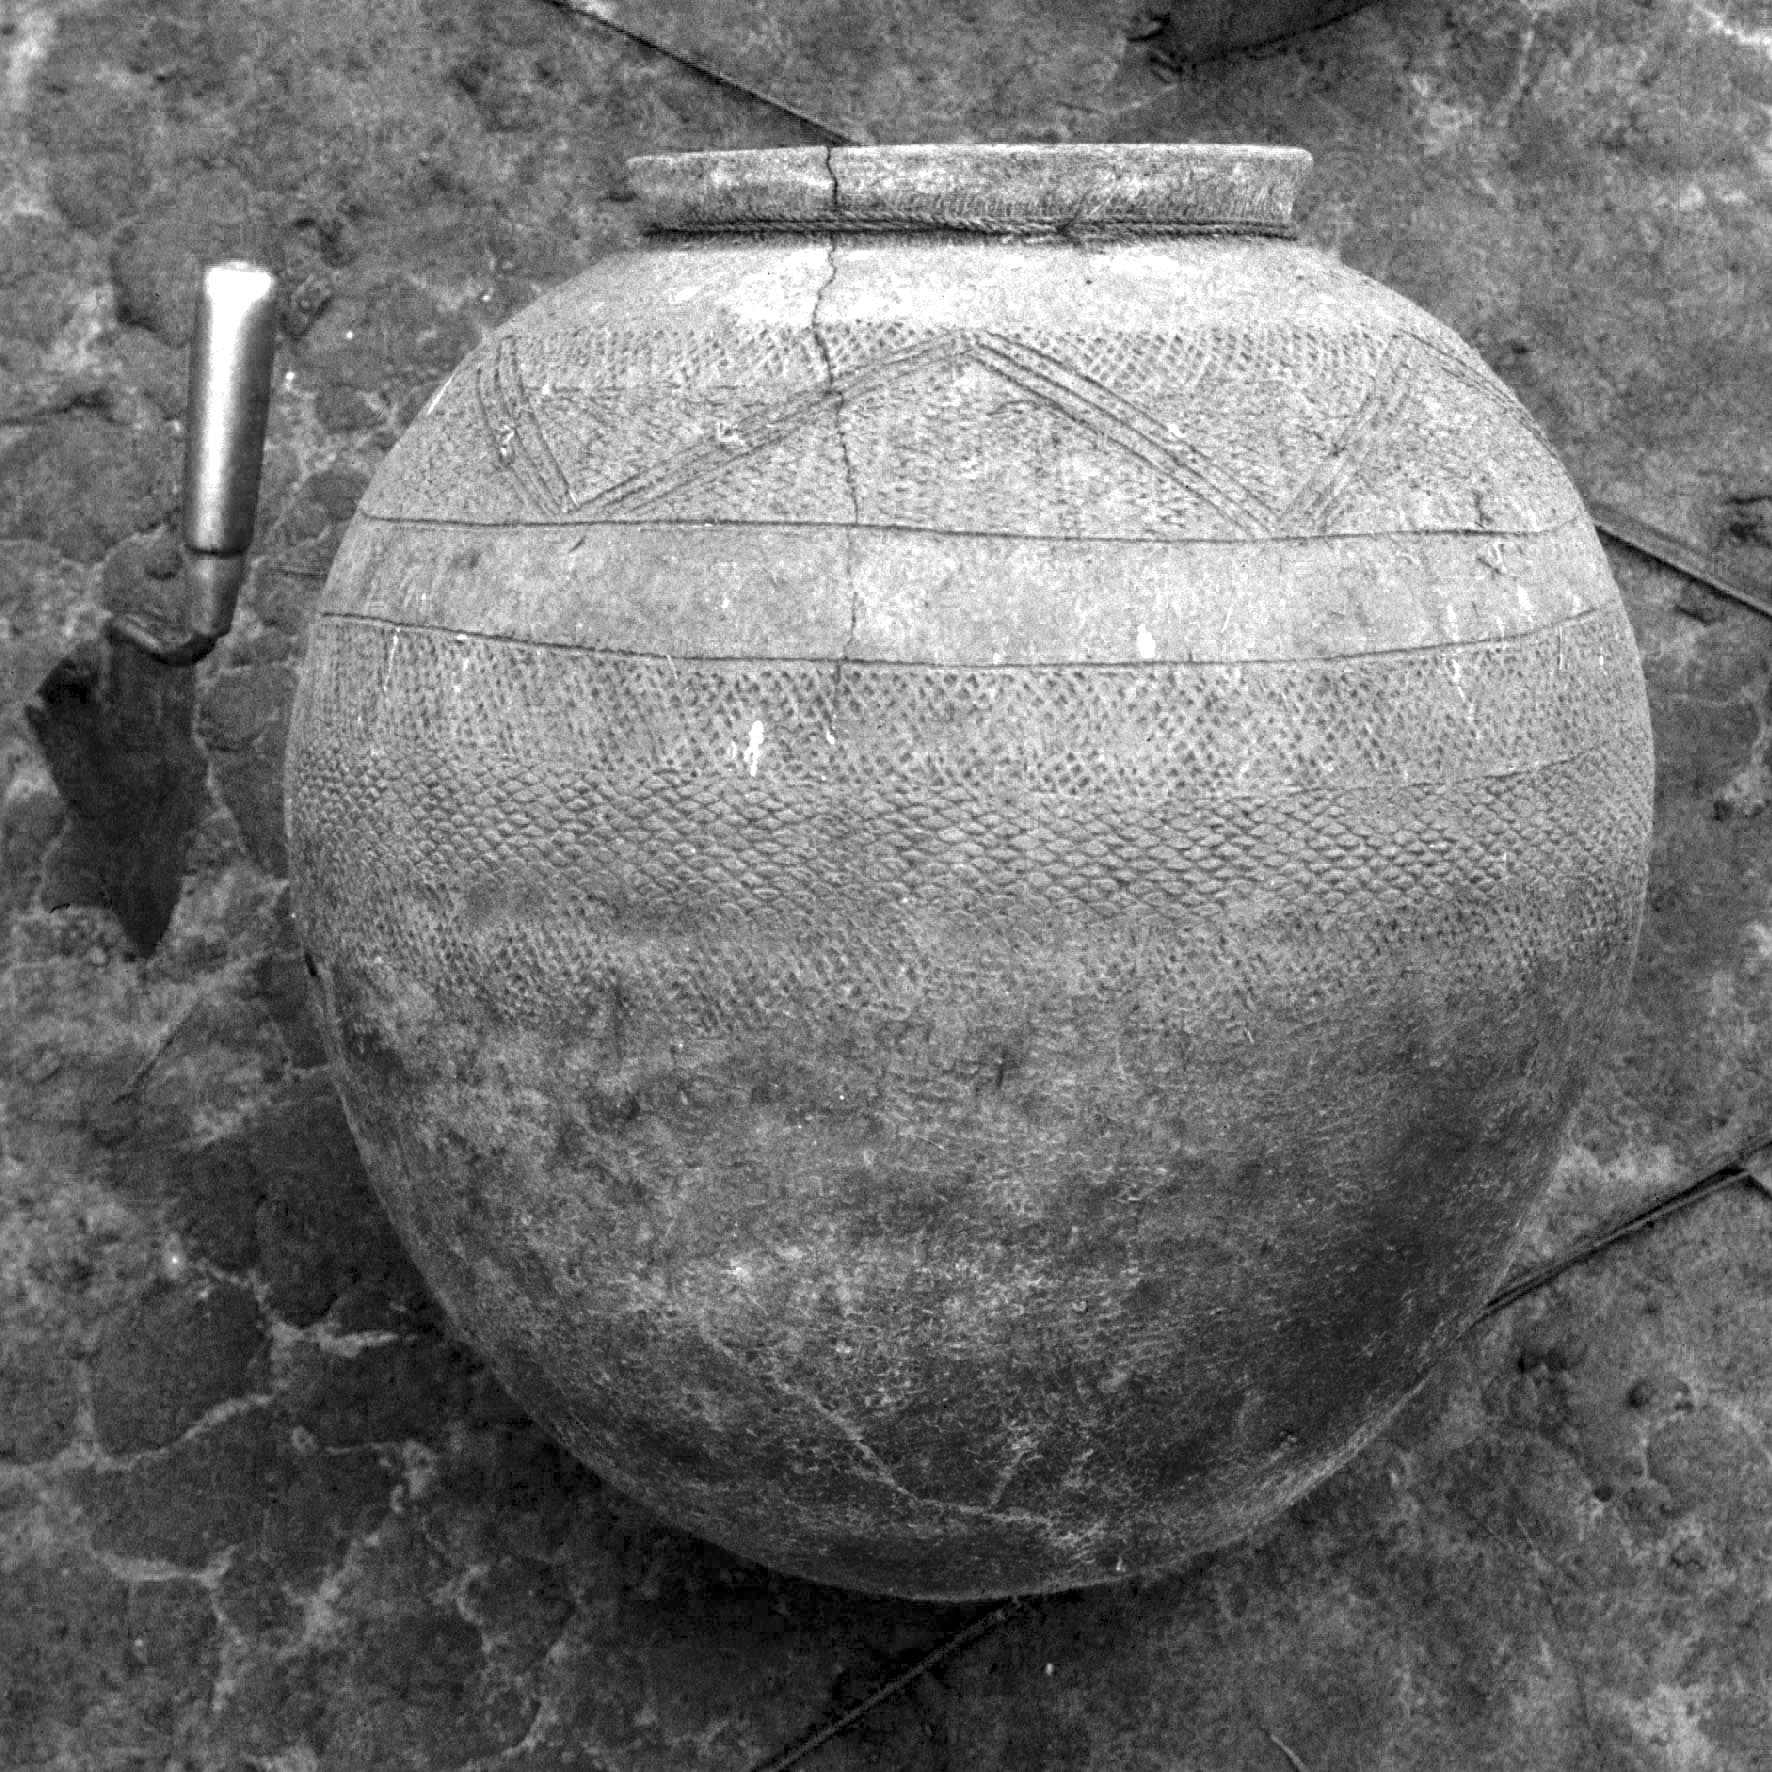
\includegraphics[width=\columnwidth]{fig/KPT85-101_Gef_E85-024-9.jpg}
		\caption{Gefäß mit konvexer Wandung und kurzem, ausbiegendem Rand (Foto: M. K. H. Eggert, 1985).}
		\label{fig:KPT85_Foto-Gef}
	\end{subfigure}\hfill
	\begin{subfigure}[b]{\columnwidth}
		%\centering
		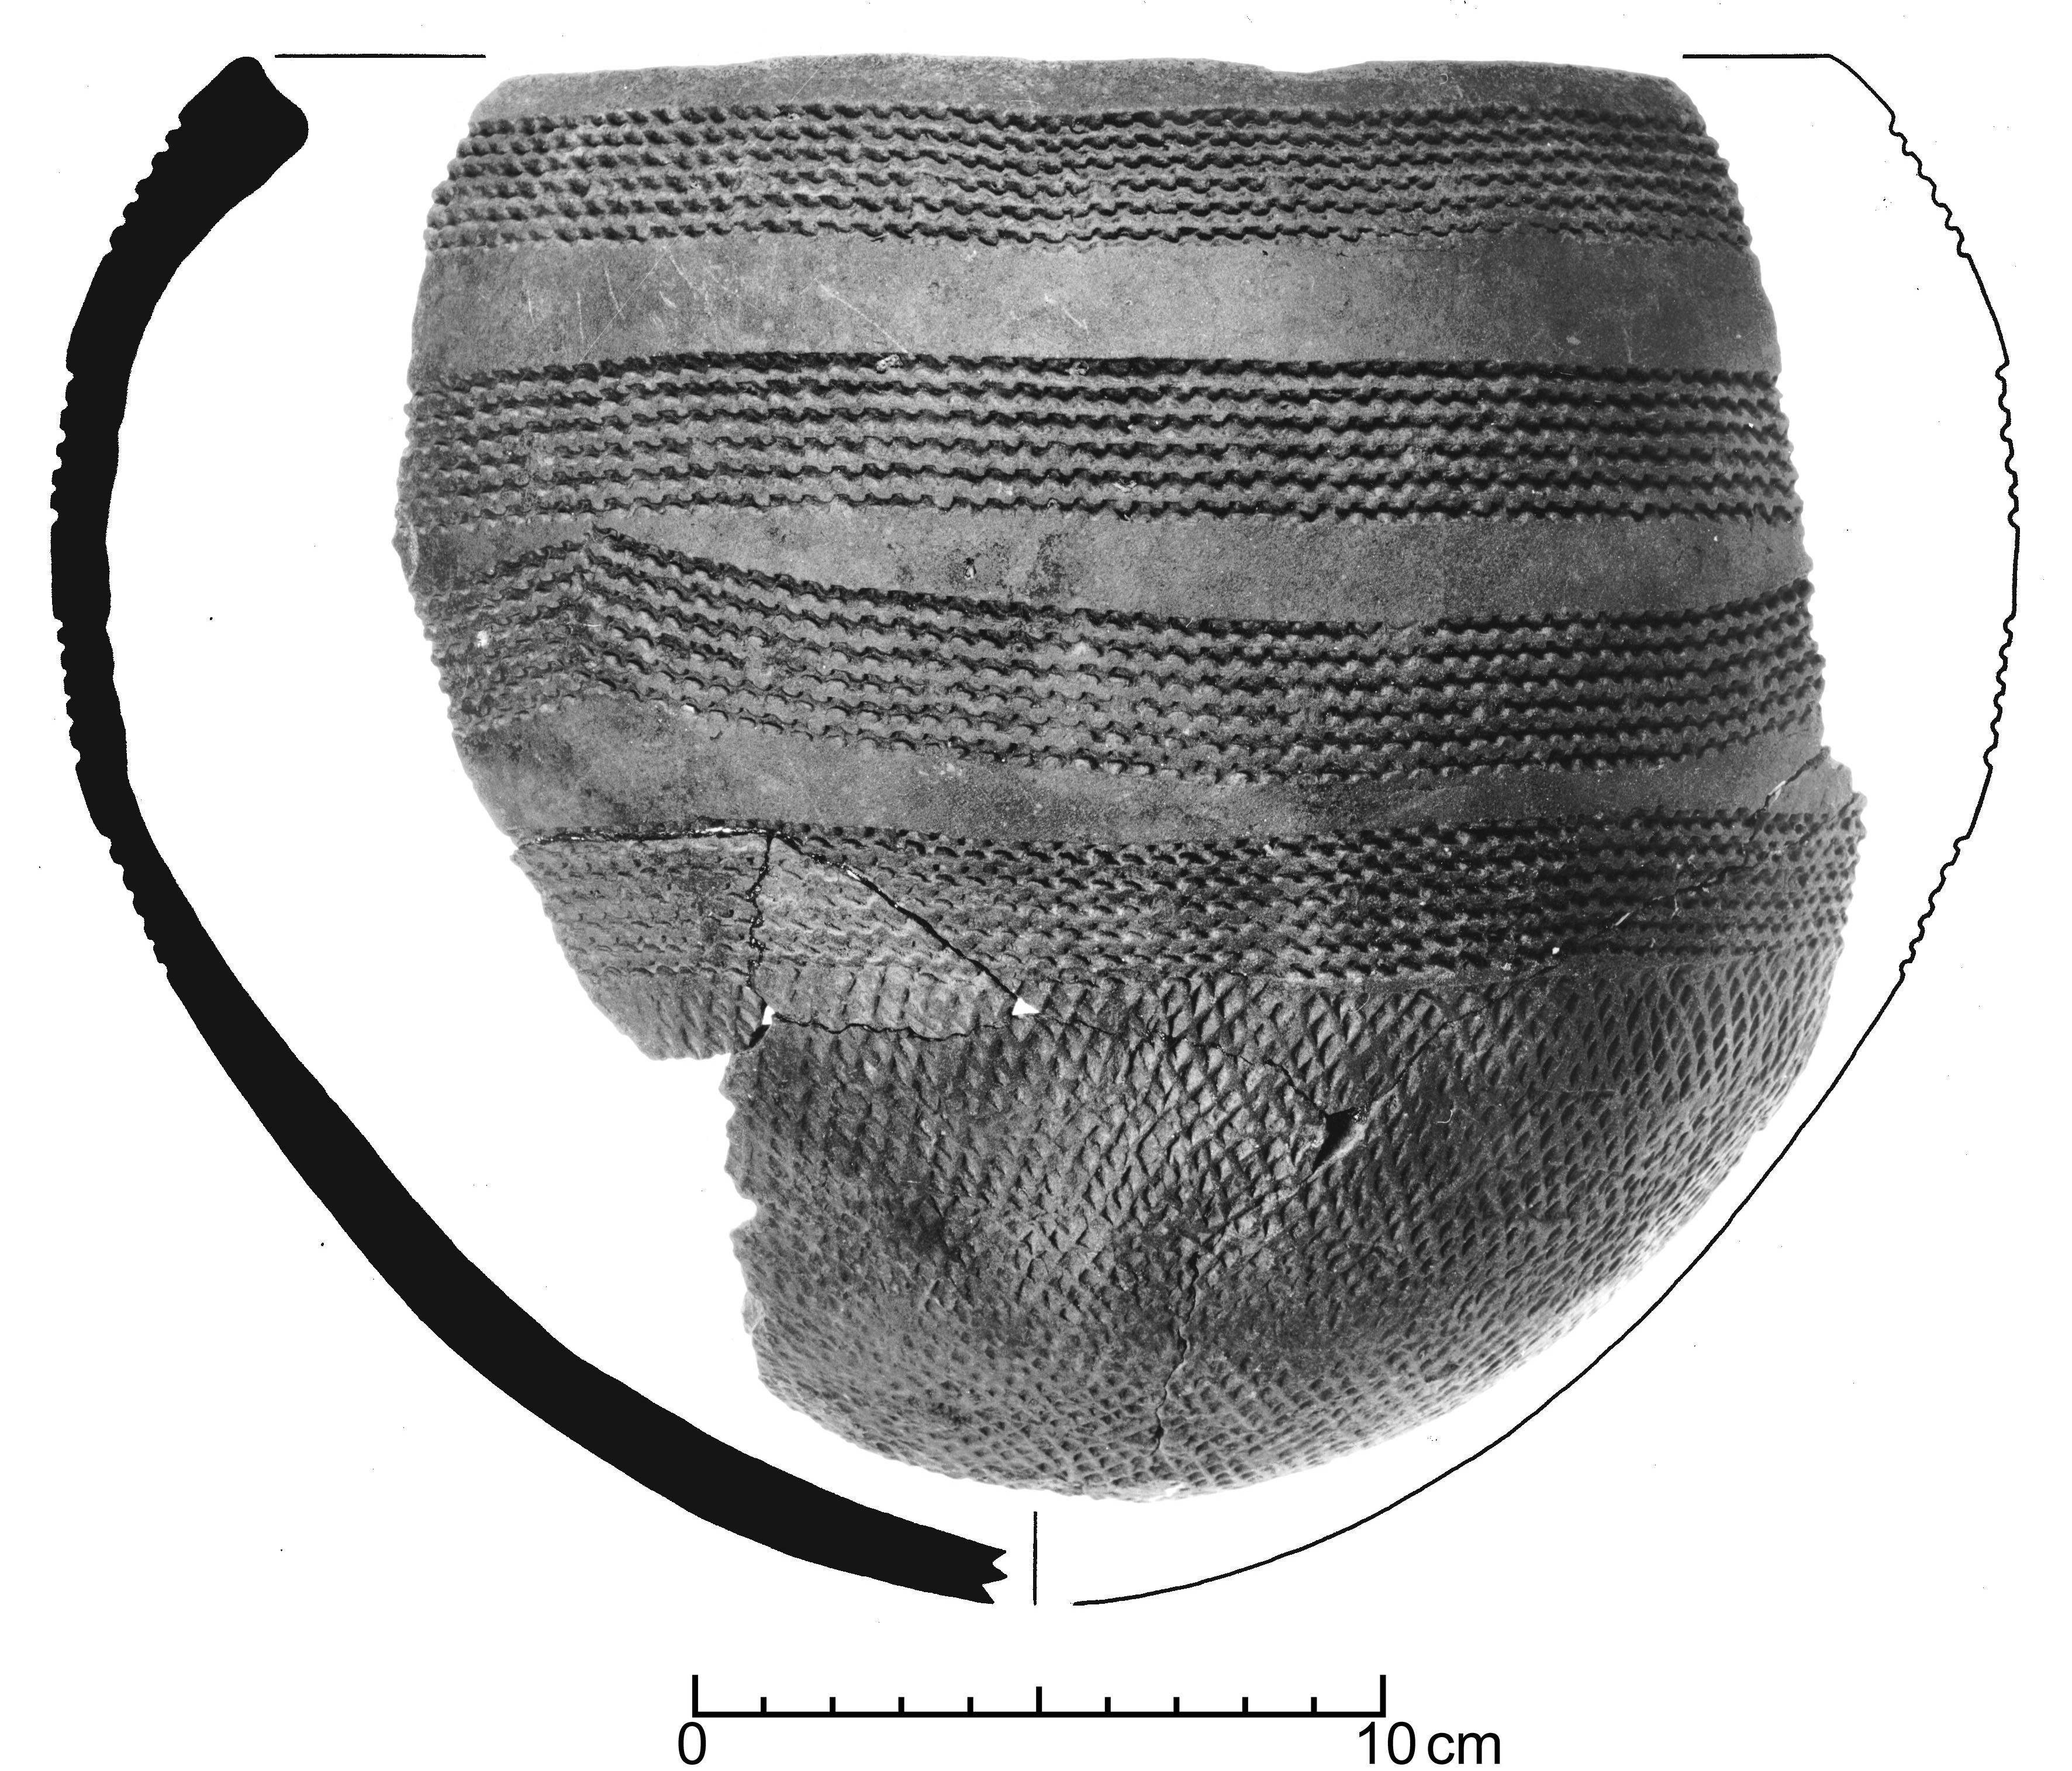
\includegraphics[width=\columnwidth]{fig/KPT85-101-10_M1-2_M.jpg}
		\caption{Schalenförmiges Gefäß mit konvexer Wandung und einbiegendem Rand (H1; Taf.~22.1).}
		\label{fig:KPT85-101-Gef}
	\end{subfigure}
	\caption{Kpetene (Fpl.~220): Gefäße der Kpetene-Gruppe.}
	\label{fig:KPT85_Typvertreter}
\end{figure*}

\subsubsection{Kpetene-Gruppe}\label{sec:KPT-Gr}

Die Kpetene-Gruppe umfasst wenige rouletteverzierte Gefäße und Gefäßfragmente, die am oberen \mbox{Ubangi} gefunden wurden (Abb.~\ref{fig:KPT_Verbreitung}). Lediglich acht GE konnten der Stilgruppe zugewiesen werden, wobei in lediglich drei Fällen eine Zuweisung zweifelsfrei möglich war. Daher kann im Fall der Kpetene-Gruppe auch nicht von einer Stilgruppe im engeren Sinne gesprochen werden. Die aus mehreren Schnitzroulette-Bändern bestehende Verzierung grenzt die hier entsprechend zusammengefassten Stücke jedoch ebenso deutlich wie die auffällig Glimmer-haltigen \textit{Fabrics} von den sonstigen rezenten Töpfereierzeugnissen am oberen \mbox{Ubangi} ab (Kap.~\ref{sec:DAM-Gr}--\ref{sec:BAN-Gr}). Die wenigen Stücke weisen neben Gemeinsamkeiten durchaus eine interne Variation auf und die zu beobachtende Verbreitung (Abb.~\ref{fig:KPT_Verbreitung}) legt nahe, das es sich nicht um ein auf einen einzelnen Platz isoliertes Phänomen handelt (siehe Kap.~\ref{sec:SHG-LKW_Einzelfunde}). Die Kpetene-Gruppe ist folglich, auch mit Blick auf die Möglichkeit, dass ein verbesserter Forschungsstand in der Zukunft eine umfassendere Definition zulässt, als Provisorium konzipiert und hier aus Gründen der terminologischen Einheitlichkeit im Detail beschrieben.\footnote{Siehe Anm.~\ref{ftn:ProvisorischeStilGr}.}

\paragraph{Technologische Merkmale}\hspace{-.5em}|\hspace{.5em}%
Die wenigen Stücke der Kpetene-Gruppe zeichnen sich durch einen Scherben aus, der größere Anteile nichtplastischer Partikel der Korngrößen \textit{coarse} und \textit{very coarse} enthält. Regelhaft handelt es sich um Quarzsand sowie Glimmer und ausgebrannte Organik. In zwei Fällen konnten auch geringe Anteile Schamott in den Scherben beobachtete werden. Die genutzten Tone sind häufig rotbrennend, nur eine GE deutet die Nutzung weißbrennender Tone an. Die Oberflächen der Scherben sind häufig geglättet.

\paragraph{Formen}\hspace{-.5em}|\hspace{.5em}%
Vier der Kpetene-Gruppe zugewiesenen GE sind rund- bis spitzbodige hohe schalenförmige Gefäße mit einbiegenden Rändern (Typ H1; Abb.~\ref{fig:KPT85-101-Gef}). Bei zwei weiteren GE blieb unklar, ob es sich um eine eher flache Variante der gleichen Grundform handelt (Typ H2). Eine Ausnahme bildet ein am eponymen Fundplatz Kpetene fotografiertes Gefäß (Abb.~\ref{fig:KPT85_Foto-Gef}). Es handelt sich um ein rundbodiges, stark bauchiges Gefäß ohne ausgeformten Halsbereich, das über einen kurzen, leicht ausbiegenden Rand verfügt (D2). Mit den anderen GE der Kpetene-Gruppe hat es die langovale Grundform mit rundem Boden und eine aus mehreren Bändern bestehende Rouletteverzierung gemein.

Die rund- bis spitzbodigen Schalen der Kpetene-Gruppen zeigen regelmäßig einbiegende Ränder (C3; Abb.~\ref{fig:KPT85-101-Gef}). Lediglich das fotografierte Gefäß verfügt über einen kurzen, ausbiegenden Rand (B1; Abb.~\ref{fig:KPT85_Foto-Gef}). Die Mündungen sind regelmäßig schräg nach innen abgestrichen (M6). Zwei GE weisen gerillte Randlippen auf (M4).

Lediglich bei einer GE konnte die Form des Bodens beobachtet werden. Es handelte sich um einen leicht spitzen Rundboden. Die fotografierte GE aus Kpetene zeigt ebenfalls einen runden, leicht spitz zulaufenden Boden (Abb.~\ref{fig:KPT85_Foto-Gef}).

\begin{figure*}[p]
	\centering
	\includegraphics[width=\textwidth]{fig/KPT_Verbreitung.pdf}
	\caption{Kpetene-Gruppe: Verbreitung.}
	\label{fig:KPT_Verbreitung}
\end{figure*}

\paragraph{Verzierungen}\hspace{-.5em}|\hspace{.5em}%
Durch die Nutzung verschiedener Verzierungstechniken werden die dem Kpetene-Stil zurgerechneten Gefäße regelhaft in einen unteren sowie einen oberen Teil untergliedert. Während der untere Teil flächigen Mattenabdruck (Tab.~\ref{tab:Verzierungselemente}: 12) zeigt, weist der obere Teil horizontale, alternierende Bänder aus Schnitzroulette auf (Abb.~\ref{fig:KPT85_Typvertreter}). Die gebänderte Verzierung der Gefäßoberteile kann neben verschiedenen Schnitzroulette-Variationen auch Ritzverzierungen umfassen (Abb.~\ref{fig:KPT85_Foto-Gef}). Eine GE weist drei mit dem gleichen \mbox{Roulette} gefertigte horizontale  Bänder sowie ein bogenförmiges, girlandenartiges Band auf (Abb.~\ref{fig:KPT85-101-Gef}).

Diagnostisches Merkmal der Kpetene-Keramik sind die verschiedene Formen von Schnitzrouletteverzierung. Vegetabilisches \mbox{Roulette} wurde in keinem Fall beobachtet. Das Schnitzroulette findet sich ohne Ausnahme auf den oberen Gefäßteilen, auf dem Bauch sowie im Schulterbereich der Gefäße. Nur eine GE zeigt auch Schnitzroulette auf dem Rand. In seltenerem Maße treten auch horizontale Rillen auf (Tab.~\ref{tab:Verzierungselemente}: 02.1; 15\,\%). Sehr viel seltener lassen sich im Material horizontale Bänder aus feinen Eindrücken beobachten (Tab.~\ref{tab:Verzierungselemente}: 04.16; 8\,\%; Abb.~\ref{fig:KPT85-101-Gef}).

\paragraph{Datierung}\hspace{-.5em}|\hspace{.5em}%
Für die innerhalb des Kpetene-Stils subsumierten keramischen Formen liegen keine absoluten Datierungen vor. Jedoch unterstreicht die Beobachtung eines noch in Benutzung befindlichen Gefäßes am eponymen Fundplatz Kpetene (Fpl. 220; Abb.~\ref{fig:KPT85_Foto-Gef}) am oberen \mbox{Ubangi} zum Zeitpunkt der Befahrung im Jahr 1985 den rezenten Charakter des entsprechenden Materials. Mit Blick auf die Schnitzroulette-Bänder zeigt das Material gewisse Ähnlichkeiten zu jener Keramik, die im Westen der Zentralafrikanischen Republik, in Nana-Modé ausgegraben wurde \parencite[34 Abb.~7,1,3--6]{David.1977}. Auch dieses Material umfasst Gefäße mit horizontalen sowie girlandenartigen Schnitzroulettebändern. Das Material der Kpetene-Gruppe setzt sich von der rezenten, schnitzrouletteverzierten Keramik der Dama-Gruppe (Kap.~\ref{sec:DAM-Gr}) sowohl durch seine ornamentalen (flächige anstatt lediglich einzelne Bänder im Schulterbereich) als auch seine morphologischen Eigenheiten (spitzbodige hohe  Gefäßtypen) ab. Von der ebenfalls rezenten Mbati-Ngombe-Keramik (Kap.~\ref{sec:MBN-Gr}), die ähnliche Gefäßformen zeigt, unterscheidet sie sich durch die Verwendung von Schnitz- anstatt vegetabilischer Roulette.

\paragraph{Verbreitung}\hspace{-.5em}|\hspace{.5em}%
Das Material der Kpetene-Gruppe wurde an fünf Fundplätzen entlang dem oberen \mbox{Ubangi}, stromauf von Bangui gefunden (Abb.~\ref{fig:KPT_Verbreitung}). Zweifelsfrei zuweisbare Stücke fanden sich lediglich in der namensgebenden Fundstelle Kpetene (Fpl.~220), in Gbandami (Fpl.~226) und in Kouango (Fpl.~229). 

\subsubsection{Dama-Gruppe}\label{sec:DAM-Gr}

Die Dama-Gruppe bildet die rezente schnitzrouletteverzierte Keramik des oberen \mbox{Ubangi} ab. Die Herstellung von Gefäßen dieser Gruppe wurde 1985 durch das \textit{River Reconnaissance Project} an der namensgebenden Fundstelle Dama~I (Fpl.~222) sowie in Boduna (Fpl.~225) und Sidi (Fpl.~228) beobachtet.\footnote{Die starken Ähnlichkeiten der Keramik aus Dama~I zu jener aus Sidi wurden bereits während der Befahrung des \mbox{Ubangi} registriert. Neben den formalen Entsprechungen wies Eggert in seinem Feldbuch (29.\,08.\,1985), ausgehend von einem Hinweis von C. Kanimba Misago, auf die ähnliche Herstellungstechnik hin. An beiden Orten erfolgt die Ausformung des Gefäßkörpers in einer kleinen Erdmulde mittels eines Stempels. Siehe Anm.~\ref{ftn:EthnoToepfereiInVorb}.} Die Beschreibung der Stilgruppe gründet auf 33~GE von 15 Fundstellen aus einem relativ großen Verbreitungsgebiet, dass von Bousoka-Mangombe (Fpl.~200) im Süden bis Kouango (Fpl. 229) im Norden reicht (Abb.~\ref{fig:DAM_Verbreitung}). Charakteristika der Stilgruppe sind runde Böden, geschlossene Gefäße mit geschweifter Wandung sowie lediglich aus einem horizontalen Schnitzroulette-Band bestehende Verzierungen (Abb.~\ref{fig:DAM_Typvertreter}). Mit Ausnahme einer im Zuge der Untersuchung des Befundes MLB~85/1-3-1 (Kat.-Nr.~1) in Maluba am Lua (Fpl.~230) gefundenen GE stammen alle Funde aus Absammlungen rezenter Dorfflächen oder wurden als Ethnographica angekauft. Die Inventare der Dama-Gruppe setzen sich vor allem aus Randscherben (60\,\%) zusammen, weisen aber auch insgesamt fünf vollständige Gefäße auf. Letztere wurden am eponymen Fundort Dama~I am \mbox{Ubangi} (Fpl.~222) angekauft.

\begin{figure*}[tb]
	\centering
	\includegraphics[width=\textwidth]{fig/DAM-Typen.pdf}
	\caption{Dama-Gruppe: Typvertreter.\\1:~Taf.~22.3; 2:~Taf.~24.1; 3:~Taf.~22.2; 4:~Taf.~12.16; 5:~Taf.~23.8; 6:~Taf.~22.4; 7:~Taf.~23.6; 8:~Taf.~23.5.}
	\label{fig:DAM_Typvertreter}
\end{figure*}

\paragraph{Technologische Merkmale}\hspace{-.5em}|\hspace{.5em}%
Die Scherben der Dama-Gruppe zeichnen sich durch ihre hohen Anteile nichtplastischer Partikel aus. Es handelt sich vornehmlich um heterogene Mischungen aus Quarzsand, in einigen Fällen wurde auch ausgebrannte Organik, Glimmer und Laterit beobachtet. Die Partikel sind ausschließlich den Größenklassen \textit{medium} (19\,\%), \textit{coarse} (32\,\%) sowie \textit{very coarse} (48\,\%) zuzurechnen. Nur wenige der Stücke (17\,\%) deuten die Nutzung weißbrennender Tone an, während ein größerer Teil eine rote Brennfarbe des Tons (34\,\%) anzeigt. Beim Gros der GE (49\,\%) ließ sich aufgrund der beigen oder grauen Färbung nicht direkt auf die Brennfarbe des genutztes Tones schließen. Die Oberflächen der meisten Scherben sind glatt (82\,\%). Nur sehr wenige Stücke zeigen eine leicht raue Oberfläche. Die Wandungsdicke der Scherben liegt im Mittel bei 7,6\,mm.

\begin{figure*}[p]
	\centering
	\includegraphics[width=\textwidth]{fig/DAM_Verbreitung.pdf}
	\caption{Dama-Gruppe: Verbreitung.}
	\label{fig:DAM_Verbreitung}
\end{figure*}

\paragraph{Formen}\hspace{-.5em}|\hspace{.5em}%
Bei 20~GE der Dama-Gruppe konnte die Gefäßform angesprochen werden. Neben stark rundbauchigen Gefäßen mit kurzem Hals (Typ D; 50\,\%; Abb.~\ref{fig:DAM_Typvertreter}.2, 6, 8) zeichnet sich die Stilgruppe durch flache Gefäße mit geschweifter Wandung, leichtem Zylinderhals und kurzen, ausbiegenden Rändern aus (Typ E; 45\,\%; Abb.~\ref{fig:DAM_Typvertreter}.1, 3, 4). Lediglich eine GE wurde als flaches Gefäß mit abknickender Wandung angesprochen (Typ F). Die GE der Dama-Gruppe zeigen eine deutliche Variabilität bei der Randgestaltung. Gerade abgestrichene Randlippen (M3; 26\,\%) kommen nur etwas häufiger vor als runde (M1; 22\,\%) oder gerillte Randabschlüsse (22\,\%). Die Ränder sind kurz konkav (B2; 23\,\%; Abb.~\ref{fig:DAM_Typvertreter}.1,3) oder gerade ausgbiegend (B1; 15\,\%; Abb.~\ref{fig:DAM_Typvertreter}.2). In geringerem Rahmen finden sich parallel aufsteigende (A1; 12), umgelegte (A2; 12\,\%), im Profil dreieckig verdickte (A2.3; 12\,\%) oder einbiegende Ränder (C1; 12\,\%). Nur in einzelnen Fällen ließen sich auch kurze konkav ausbiegende (B2.1; 8\,\%), verdickte (A4, 4\,\%) sowie konvex ausbiegende Ränder feststellen (B3; 4\,\%). Die Hälfte der GE zeigt einen konkav ausgearbeiteten Halsbereich, während der Schulterbereich entweder gerade oder konvex geformt ist. Der überwiegende Teil der GE zeigt lang ausgeführte Halsbereiche (89\,\%). Bei drei GE der Dama-Gruppe konnte die Bodenform angesprochen werden. Während eines der Gefäße aus Dama~I einen runden Boden aufweist (B1; Abb.~\ref{fig:DAM_Typvertreter}.3), ist der Boden des zweiten auffallend flach (B4; Abb.~\ref{fig:DAM_Typvertreter}.1).\footnote{Mit Blick auf die in Dama~I beobachtete Herstellung der beiden Gefäße durch Abformen in einer kleinen Erdkuhle könnte der flache Boden auch auf eine unbeabsichtigte Variation während des Herstellungsprozesses zurückgehen. Während des Töpferns wurde zu keinem Zeitpunkt die Ausarbeitung eines dediziert flachen Bodens beobachtet.} Eine dritte, aus Bousoka-Mangombe (Fpl.~200) stammende GE zeigt ebenfalls einen runden Boden (B1).

\paragraph{Verzierungen}\hspace{-.5em}|\hspace{.5em}%
Die Keramik der Dama-Gruppe zeichnet sich durch eine regelhafte Schnitzrouletteverzierung aus. Die verschiedenen Variationen machen zusammen 70\,\% der beobachteten Verzierungselemente aus. Daneben wurden fast ausschließlich horizontale Rillen beobachtet (Tab.~\ref{tab:Verzierungselemente}: 02.1; 28\,\%), die sich auf allen Gefäßteilen von der Innenseite der Ränder bis zum Gefäßbauch fanden (Anlage~4\subref{fig:DAM_Verz}). Daneben ließen sich lediglich in sehr geringen Anzahlen kleine, vertikale Eindrücke beobachten (Tab.~\ref{tab:Verzierungselemente}: 04.15; 2\,\%). Die Rouletteverzierung wurde regelhaft als einzelnes Band auf der Schulter oder dem Bauchbereich der Gefäße aufgebracht, seltener auch auf der Innenseite des Randes (Abb.~\ref{fig:DAM_Typvertreter}.4) oder außen am Rand (Abb.~\ref{fig:DAM_Typvertreter}.8). Die häufigste Schnitzroulette-Variante erzeugt ein \textit{erhabenes} rautenförmiges Muster (Tab.~\ref{tab:Verzierungselemente}: 21.7; 40\,\%), gefolgt von einer ganz ähnlichen Variante, bei der ein aus eingetiefeten Rauten bestehendes Muster entsteht (Tab.~\ref{tab:Verzierungselemente}: 21.10; 9\,\%). Das bei der Motenge-Boma-Gruppe (Kap.~\ref{sec:MTB-Gr}) häufige tannenbaumartige Schnitzroulette fand sich an den GE der Dama-Gruppe deutlich seltener (Tab.~\ref{tab:Verzierungselemente}: 21.12; 7\,\%). Ebenfalls beobachtet werden konnten Roulettes mit gezähnten tiefen Einschnitten (Tab.~\ref{tab:Verzierungselemente}: 21.5--6; 10\,\%) sowie eine komplexere, rautenförmige Muster erzeugende Variante (Tab.~\ref{tab:Verzierungselemente}: 21.8; 5\,\%). Anders als innerhalb der Motenge-Boma- (Kap.~\ref{sec:MTB-Gr}) sowie Kpetene-Gruppe (Kap.~\ref{sec:KPT-Gr}) wird bei der Dama-Keramik fast ausschließlich ein einzelnes horizontales Band im Schulterbereich in  Roulettetechnik aufgebracht. Flächige Muster lassen sich nicht beobachten. Die Unterteile und Standflächen der Dama-Gefäße sind durchweg unverziert (Anlage~4\subref{fig:DAM_Verz}).

\paragraph{Datierung}\hspace{-.5em}|\hspace{.5em}%
Die Keramik der Dama-Gruppe bildet das rezente keramische Spektrum am oberen \mbox{Ubangi} ab. Die Datierung des Materials basiert auf der Beobachtung der Herstellung dieser Keramik in Dama~I (Fpl.~222) sowie Sidi (Fpl.~228) bei den Prospektionen von 1985. Eine Scherbe, welche der Dama-Gruppe zugerechnet werden kann, wurde überdies bei der Grabung der Grube MLB~85/1-3-1 (Kat.-Nr.~1) in Maluba am Lua (Fpl.~230) im ersten Abtrag angetroffen.\footnote{Es ist auffällig, dass die entsprechenden Tafeln zeitgenössischer Keramik aus dem \textit{État Indépendant du Congo}, die sich im Besitz des damaligen \textit{Musée du Congo} befand \parencite[Taf.~XIV--XV]{Coart.1907}, keine rouletteverzierte Keramik aus dem Bereich des \mbox{Ubangi} zeigen.\label{ftn:Coart1907RouletteUbangi}}

\paragraph{Verbreitung}\hspace{-.5em}|\hspace{.5em}%
Die Keramik der Dama-Gruppe fand sich in einem nur vage eingrenzbaren Gebiet entlang des mittleren und oberen Laufes des \mbox{Ubangi} sowie des befahrenen Abschnitts des Lua (Abb.~\ref{fig:DAM_Verbreitung}). Eine dichte Belegung kann für das direkte Umfeld der drei Töpfereidörfer Dama~I (Fpl.~222), Boduna (Fpl.~225) und Sidi (Fpl.~228) beobachtet werden. Eine weitere Konzentration von der Dama-Gruppe zuordenbarer GE fand sich im Bereich des Lua und seiner Mündung in den \mbox{Ubangi}. Zwei GE fanden sich auch deutlich weiter südlich in Bousoka-Mangombe (Fpl. 200). Auffällig an diesem Verbreitungsgebiet ist, dass die Lücke zwischen den beiden im Fundgut beobachteten Hauptverbreitungsgebieten der Dama-Gruppe teilweise durch die Anwesenheit von Funden der ebenfalls rezenten Stilgruppen Mbati-Ngombe (Kap.~\ref{sec:MBN-Gr}; Abb.~\ref{fig:MBN_Verbreitung}) und Bangui (Kap.~\ref{sec:BAN-Gr}; Abb.~\ref{fig:BAN_Verbreitung}) aufgefüllt wird.

\begin{figure*}[tb]
	\centering
	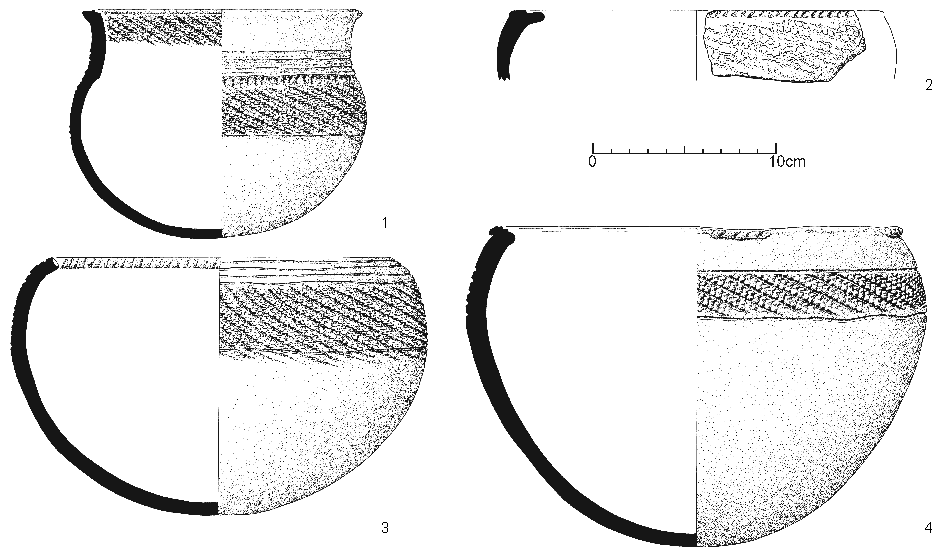
\includegraphics[width=\textwidth]{fig/MBN-Typen.pdf}
	\caption{Mbati-Ngombe-Gruppe: Typvertreter.\\1:~Taf.~10.10; 2:~Taf.~27.11; 3:~Taf.~10.9; 4:~Taf.~10.11.}
	\label{fig:MBN_Typvertreter}
\end{figure*}

\subsubsection{Mbati-Ngombe-Gruppe}\label{sec:MBN-Gr}

Die Mbati-Ngombe-Gruppe beschreibt eine rezente, vegetabilische Roulettes verwendende Keramik, die vor allem am mittleren \mbox{Ubangi} sowie am prospektierten Teil des Lua zu finden ist (Abb.~\ref{fig:MBN_Verbreitung}). Am eponymen Fundort am mittleren \mbox{Ubangi} (Fpl.~204) wurde die Herstellung mehrerer Gefäße beobachtet und dokumentiert.\footnote{Siehe Anm.~\ref{ftn:EthnoToepfereiInVorb}.} Insgesamt vier Gefäße wurden angekauft (Abb.~\ref{fig:MBN_Typvertreter}.1,3--4). Die Stilgruppe umfasst 24~GE aus 14 unterschiedlichen Fundstellen. Keine der Mbati-Ngombe-Gruppe zurechenbare GE stammt aus einer Grabung. Das Material wurde sämtlich von rezenten Dorfflächen abgesammelt oder als \textit{Ethnographica} angekauft. Bestimmende Charakteristika der Inventare sind flache Gefäße mit geschweifter Wandung (Abb.~\ref{fig:MBN_Typvertreter}.1), wie sie auch in der ebenfalls rezenten Dama-Gruppe vorkommen (Kap.~\ref{sec:DAM-Gr}) und schalenförmige Gefäße mit konvexer Wandung und einbiegendem Rand (Abb.~\ref{fig:MBN_Typvertreter}.2--4), wie sie von der Kpetene-Gruppe bekannt sind (Kap.~\ref{sec:KPT-Gr}), sowie eine Verzierungspraxis, die sich lediglich durch die Nutzung vegetabilischer Roulettes von der der Dama-Keramik unterscheidet. Die Beschreibung der Mbati-Gombe-Gruppe basiert vornehmlich auf sechs kompletten Gefäßen (25\,\%) und einer Reihe von Randstücken (58\,\%). 


\paragraph{Technologische Merkmale}\hspace{-.5em}|\hspace{.5em}%
Aus technischer Sicht entsprechen die GE der Mbati-Ngombe-Gruppe den zeitgleichen keramischen Inventaren am mittleren und oberen \mbox{Ubangi}. Die Scherben enthalten fast ausschließlich hohe Anteile heterogener Quarzsande (74\,\%) und nur selten Schamott oder rötliche Partikel, bei denen es sich um zerstoßenen Laterit handeln könnte. Die Partikel gehören größtenteils der Größenklasse \textit{coarse} an (65\,\%), während kleinere (\textit{medium}) sowie größere Korngrößen (\textit{very coarse}) in gleichem Maße vorkommen (je 17\,\%). Bei den \textit{Fabrics} zeigt sich eine gewisse Heterogenität, da die Typen 3c, 4c und 5a zu gleichen Anteilen beobachtet wurden (je 17\,\%). Nur etwas seltener konnte das \textit{Fabric} 4a beobachtet werden (13\,\%). Zudem zeigen nur wenige der Stücke (13\,\%) die Nutzung weißbrennender Tone an, während sich das Gros (48\,\%) aufgrund grauer, beiger oder schwarzer Färbung nicht näher ansprechen lässt. Eine nicht unerhebliche Zahl der GE weist jedoch auf die Nutzung rotbrennender Tone hindeutende Färbungen auf (40\,\%). Die Oberflächen der meisten Scherben sind glatt (70\,\%) oder nur leicht rau (26\,\%).

\begin{figure*}[p]
	\centering
	\includegraphics[width=\textwidth]{fig/MBN_Verbreitung.pdf}
	\caption{Mbati-Ngombe-Gruppe: Verbreitung.}
	\label{fig:MBN_Verbreitung}
\end{figure*}

\paragraph{Formen}\hspace{-.5em}|\hspace{.5em}%
Im Fall von 19~GE war eine Ansprache der Gefäßform möglich. Aufgrund der Fragmentierung der Stücke aus den Oberflächenabsammlungen war nur bei etwas über der Hälfte eine sichere Bestimmung möglich. Zu gleichen Anteilen finden sich flache Gefäße mit geschweifter Wandung und ausgeprägtem Gefäßhals (Typ E; 37\,\%) und schalenförmige Gefäße mit konvexer Wandung und einbiegendem Rand (Typ H; 37\,\%; Abb.~\ref{fig:MBN_Typvertreter}.2--4). Innerhalb der flachen Gefäße mit geschweifter Wandung findet sich vornehmlich der Typ E2 (24\,\%; Abb.~\ref{fig:MBN_Typvertreter}.1). Lediglich eine GE war als Flasche ansprechbar (Typ A; 5\,\%). Die Randgestaltung der Mbati-Ngombe-Gefäße ist, ähnlich wie im Fall der Dama-Gruppe (Kap.~\ref{sec:DAM-Gr}) sehr variabel. Die Randabschlüsse sind vornehmlich rund ausgeformt (M1; 47\,\%). Seltener fanden sich spitze (M2; 16\,\%) oder gerillte Randlippen (M4; 10\,\%). Die häufigste Randform sind konvex einbiegende Ränder (C3; 37\,\%; Abb.~\ref{fig:MBN_Typvertreter}.3), die sich auschließlich an schalenförmigen Gefäßen mit konvexer Wandung (H) finden. Daneben kommen konkav ausbiegende Ränder (B2; 16\,\%; Abb.~\ref{fig:MBN_Typvertreter}.1), einfach ausbiegende (B1; 11\,\%), umgelegte (A2; 11\,\%) sowie einfach einbiegende Ränder vor (C1; 11\,\%). Die flachen Gefäße mit geschweifter Wandung weisen durchweg konkav ausgearbeitete oder zylindrische Hälse auf. Die Schulterbereiche der Gefäße, die eine ausgearbeitete Schulter aufweisen, sind fast ausschließlich konvex (75\,\%) oder gerade (12\,\%) ausgeformt. Nur eine GE zeigt einen Schulterabsatz. Die Gefäßkörper sind mit Ausnahme einer GE deutlich konvex ausgeformt (93\,\%). Bei fünf GE war es möglich, einen runden Gefäßboden zu identifizieren. Eine Ausnahme bildet eine GE vom eponymen Fundplatz Mbati-Ngombe (Fpl.~204), die einen Flachboden mit konkaver Standfläche aufwies (Taf.~10.12).


\paragraph{Verzierungen}\hspace{-.5em}|\hspace{.5em}%
Die Verzierungspraxis der Mbati-Ngombe-Keramik setzt sich vornehmlich aus drei Gruppen von Verzierungselementen zusammen (Anlage~4.10): vegetabilisches \mbox{Roulette} (Tab.~\ref{tab:Verzierungselemente}: 21.1--3), vor allem auf der Innenseite der Ränder sowie im Schulter- und Bauchbereich, die zusammen 38\,\% aller beobachteten Verzierungselemente ausmachen, sowie Riefen (Tab.~\ref{tab:Verzierungselemente}: 02.1 und 02.4--5) und Eindrücke (Tab.~\ref{tab:Verzierungselemente}: 04.12 und 04.15--16). Das mit Abstand am häufigsten aufgenommene Verzierungselement sind einfache horizontale Riefen (Tab.~\ref{tab:Verzierungselemente}: 02.1; 45\,\%). Diese finden sich vor allem auf der Innenseite der Ränder (Abb.~\ref{fig:MBN_Typvertreter}.1,4), aber auch auf allen anderen Gefäßteilen, mit Ausnahme der Unterteile und Standflächen, die regelhaft unverziert sind. Eindrücke, die sehr selten vorkommen, finden sich wenn, dann ebenfalls vornehmlich auf der Innenseite der Ränder (Abb.~\ref{fig:MBN_Typvertreter}.3). Die charakteristische vegetabilische Rouletteverzierung wird vor allem von \textit{knotted strip}-Roulette (Tab.~\ref{tab:Verzierungselemente}: 21.1; 27\,\%) bestimmt. In deutlich geringerem Maße treten \textit{twisted string}- (Tab.~\ref{tab:Verzierungselemente}: 21.2; 9\,\%) sowie \textit{alternate knotted strip}-Roulette (Tab.~\ref{tab:Verzierungselemente}: 21.3; 2\,\%) auf. Eine Verzierung der Gefäßteile unterhalb des maximalen Durchmessers oder der Bodenbereiche ließ sich bei keiner GE der Mbati-Ngombe-Gruppe beobachten.


\paragraph{Datierung}\hspace{-.5em}|\hspace{.5em}%
Die chronologische Ansprache der Mbati-Ngombe-Keramik als rezent stützt sich vornehmlich auf die Beobachtung der Herstellung dieser Gefäße im Jahr 1985. Da keine Funde von Mbati-Ngombe-Keramik aus Ausgrabungen bekannt sind, muss dieses sehr eindeutige Datierungsindiz ausreichen, um die Stilgruppe als rezent anzusprechen.\footnote{Siehe auch Anm.~\ref{ftn:Coart1907RouletteUbangi}.}

\begin{figure*}[tb]
	\begin{minipage}[b]{.2\textwidth}
		\caption{Bangui-Gruppe: Typvertreter.\\1:~Taf.~20.7; 2:~Taf.~16.1; 3:~Taf.~21.1; 4:~Taf.~20.8.}
		\label{fig:BAN_Typen}
	\end{minipage}\hfill
	\begin{minipage}[b]{.8\textwidth}
		\includegraphics[width=\textwidth]{fig/BAN-Typen.pdf}
	\end{minipage}
\end{figure*}

\paragraph{Verbreitung}\hspace{-.5em}|\hspace{.5em}%
Das Kernverbreitungsgebiet der Mbati-Ngombe-Keramik beschränkt sich auf den mittleren Abschnitt des \mbox{Ubangi}, zwischen Imese (Fpl.~201) im Süden und Batanga (Fpl.~209) im Norden. Während sich eine fragliche GE weiter südlich in Ebeka (Fpl.~197) fand, wurde auch weiter nördlich in Kpetene (Fpl.~220) eine, der Mbati-Ngombe-Gruppe zurechenbare GE gefunden. Beide Stücke  müssen als Einzelfunde angesehen werden und zeichnen nicht das Hauptverbreitungsgebiet der Stilgruppe nach, das sich weniger als 100\,km südlich wie nördlich des eponymen Töpfereidorfes (Fpl.~204) entlang des \mbox{Ubangi} erstreckt. Weiter im Norden schließt sich das Verbreitungsgebiet der ebenfalls rezenten Bangui-Keramik (Kap.~\ref{sec:BAN-Gr}; Abb.~\ref{fig:BAN_Verbreitung}) direkt an das der Mbati-Ngombe-Gruppe an. Im Hauptverbreitungsgebiet der Mbati-Ngombe-Gruppe findet sich jedoch auch Fundgut der ebenfalls rezenten Dama-Gruppe (Kap.~\ref{sec:DAM-Gr}). Die Bedeutung dieser Beobachtung kann anhand der vorliegenden Funde nicht erschlossen werden.


\subsubsection{Bangui-Gruppe}\label{sec:BAN-Gr}

Neben Vertretern der durch die Roulettetechnick charakterisierten Stile Dama (Kap.~\ref{sec:DAM-Gr}) und Mbati-Ngombe (Kap.~\ref{sec:MBN-Gr}) wurden 1985 am Oberlauf des \mbox{Ubangi} auch eine Reihe von Gefäßen angekauft und bei Surveys gefunden, die keine Rouletteverzierung zeigen. Das als Bangui-Gruppe systematisierte Material setzt sich aus zehn GE zusammen, die sich an sieben verschiedenen Fundstellen fanden (Abb.~\ref{fig:BAN_Verbreitung}). Sicher der Bangui-Gruppe zurechenbare GE finden sich lediglich in einem kleinen Bereich zwischen Libenge im Süden (Fpl.~208) und Bangui im Norden (Fpl.~215). Eventuell der Stilgruppe zurechenbare Stücke fanden sich noch weiter flussauf, zwischen Gbandami (Fpl. 226) und \mbox{Kouango} (Fpl.~229). Neben den zwei in Balongoi (Fpl. 214; Abb.~\ref{fig:BAN_Typen}.1,4) und einer in Bangui angekauften GE (Fpl. 215; Abb.~\ref{fig:BAN_Typen}.3) stammen alle Stücke von Absammlungen rezenter Dorfflächen.

\paragraph{Technologische Merkmale}\hspace{-.5em}|\hspace{.5em}%
Die Scherben der Bangui-Keramik zeichnen sich durch einen geringeren Anteil nichtplastischer Partikel aus, die vornehmlich den Größenklassen \textit{fine} (43\,\%) sowie \textit{medium} (29\,\%) zuzurechnen sind. Die Anteile nichtplastischer Partikel im Scherben liegt in der Regel zwischen 3--5\,\% (57\,\%) und 7--10\,\% (29\,\%). Es handelt sich vornehmlich um heterogene Mischungen aus Quarz, Laterit und Glimmer. Vor allem der hohe Anteil von Glimmer in den Scherben ist auffällig. Aufgrund der kleinen Stichprobe können diese Zahlen selbstverständlich nur bedingt als repräsentativ angesehen werden. Mit Blick auf die \textit{Fabrics} ließen sich die Varianten 3c, 5c sowie 6b und 8a beobachten. Die Brennfarbe des genutzten Tons konnte in keinem Fall sicher bestimmt werden. Die Oberflächen der Stücke sind durchweg glatt, in einem Fall zeigt die Oberfläche sogar deutlich Hinweise auf eine intensive Glättung, welche als Politur angesprochen werden kann.

\begin{figure*}[p]
	\centering
	\includegraphics[width=\textwidth]{fig/BAN_Verbreitung.pdf}
	\caption{Bangui-Gruppe: Verbreitung.}
	\label{fig:BAN_Verbreitung}
\end{figure*}

\paragraph{Formen}\hspace{-.5em}|\hspace{.5em}%
Lediglich bei sechs der zehn GE der Bangui-Gruppe war eine Ansprache der Gefäßform möglich. Vier GE sind flache Gefäße mit geschweifter Wandung (Typ~E; Abb.~\ref{fig:BAN_Typen}.3--4). Ebenfalls vertreten ist ein flaschenförmiges Gefäß (Typ~A; Abb.~\ref{fig:BAN_Typen}.1) sowie ein schalenförmiges Gefäß mit konvexer Wandung (Typ~I; Taf.~24.2). Die Randlippen sind etwa zu gleichen Anteilen rund (M1), spitz (M2) oder gerade (M3) ausgearbeitet, während die Ausrichtung der Ränder grundsätzlich ausbiegend ist. Gerade (B1) sowie konkav (B2) oder konvex ausbiegende Ränder (B3) kommen etwa zu gleichen Anteilen vor. Die Halsbereiche der Gefäße sind häufig sehr kurz gehalten oder überhaupt nicht dezidiert ausgearbeitet. Bei vier GE konnte die Ausprägung des Bodens beobachtet werden. Neben zwei runden Böden (B1; Abb.~\ref{fig:BAN_Typen}.4; Taf.~24.8) wurden auch zwei flache Standböden (B4; Abb.~\ref{fig:BAN_Typen}.1,3) beobachtet.

\paragraph{Verzierungen}\hspace{-.5em}|\hspace{.5em}%
Die GE der Bangui-Gruppe zeichnen sich durch eine klare Strukturierung ihrer Verzierung aus. Auf den Unterseiten sowie Standflächen findet sich eine flächige, an \textit{banfwa-nfwa} (Tab.~\ref{tab:Verzierungselemente}: 08) erinnernde aber stellenweise auffällig irreguläre Aufrauung der Oberfläche (Tab.~\ref{tab:Verzierungselemente}: 22.2; 27\,\%; Abb.~\ref{fig:BAN_Typen}.1--3). Die oberen Gefäßteile zeichnen sich regelhaft durch horizontale Bänder runder bis leicht ovaler Eindrücke (Tab.~\ref{tab:Verzierungselemente}: 04.11; 24\,\%; Abb.~\ref{fig:BAN_Typen}.1--4) sowie horizontaler Riefen aus (Tab.~\ref{tab:Verzierungselemente}: 02.1; 26\,\%; Abb.~\ref{fig:BAN_Typen}.4).\footnote{Diese Verzierung der Gefäßoberteile durch horizontale Bänder erinnert an die Verzierungspraxis der Kpetene-Gruppe (Kap.~\ref{sec:KPT-Gr}).} Die Eindrücke können auch größere geometrische Flächen ausfüllen (Abb.~\ref{fig:BAN_Typen}.1). Ebenso ließen sich Kombinationen aus horizontalen (Tab.~\ref{tab:Verzierungselemente}: 02.1) sowie winkelförmig ausgearbeiteten Riefen-Bändern beobachten (Tab.~\ref{tab:Verzierungselemente}: 01.6 und 02.3; Abb.~\ref{fig:BAN_Typen}.3).\footnote{Die auf einer GE (Abb.~\ref{fig:BAN_Typen}.4) beobachteten bogenförmigen Riefen könnten auf eine Beziehung der Bangui-Keramik zur Mokelo-Gruppe (Kap.~\ref{sec:MKL-Gr}) hinweisen.}


\paragraph{Datierung}\hspace{-.5em}|\hspace{.5em}%
Absolute Daten für die chronologische Ansprache der Keramik des Bangui-Stils liegen nicht vor. Die beiden in Balongoi (Fpl.~214; Abb.~\ref{fig:BAN_Typen}.1,4) sowie die in Bangui (Fpl. 215; Abb.~\ref{fig:BAN_Typen}.3) als \textit{Ethnographica} angekauften GE belegen jedoch die rezente Nutzung der Gefäße und legen ein grundsätzlich zeitgenössisches Alter nahe.

Die morphologischen Eigenschaften der Bangui-Gruppe erinnern mit Blick auf die grundsätzlich rundbauchigen Gefäße, das Fehlen ausgeprägter Hals"-partien sowie das Vorhandensein kurzer, ausbiegender Ränder an die Dama-Keramik (Kap.~\ref{sec:DAM-Gr}). Die flächige \textit{Behandlung} beziehungsweise Aufrauung der Gefäßunterseiten stellt eine Parallele zur Kpetene-Gruppe dar (Kap.~\ref{sec:KPT-Gr}). Die Bänder aus Eindrücken hingegen stellen einen Bezug zur älteren Keramik der Mokelo-Gruppe (Kap.~\ref{sec:MKL-Gr}) her, die etwa in der gleichen Region verbreitet ist (Abb.~\ref{fig:MKL_Verbreitung}).

\paragraph{Verbreitung}\hspace{-.5em}|\hspace{.5em}%
Bangui-Keramik findet sich in einem kleinen Verbreitungsgebiet direkt südlich der Hauptstadt der Zentralafrikanischen Republik Bangui, die der eponyme Fundplatz für die Stilgruppe ist (Fpl.~215). Der südlichste Fundplatz von sicher als Bangui ansprechbarer Keramik ist Libenge (Fpl.~208), während der nördlichste Bangui selbst ist. Etwa 160\,km stromauf von Bangui, kurz vor dem Ende der Befahrung von 1985, fanden sich zwischen Gbandami (Fpl.~226) und Kou"-a"-ngo (Fpl.~229) GE, die möglicherweise der Bangui-Gruppe zuzuweisen sind. Eine Erklärung dieses Verbreitungsbildes kann, beruhend auf der gegenwärtig vorliegenden, sehr begrenzten empirischen Datenlage, nicht gegeben werden.\footnote{Das engere Verbreitungsgebiet zwischen Libenge (Fpl.~208) und Bangui (Fpl.~215) könnte mit begrenztem Handel der Stücke erklärt werden.}


\subsection{\mbox{Sangha}-, \mbox{Ngoko}- und Likwala-aux-Herbes-Gebiet}

\subsubsection{Pikunda-Munda-Gruppe}\label{sec:PKM-Gr}

Der Pikunda-Munda-Stil beschreibt die älteste in größerem Umfang nachweisbare Keramik im südlichen Teil des Arbeitsgebiets.\footnote{Der älteren Imbonga-Gruppe zurechenbare Stücke fanden sich lediglich in sehr begrenztem Rahmen an zwei Fundstellen am unteren \mbox{Sangha} (Kap.~\ref{sec:IMB-Gr}; Kat.-Nr.~12--13).} Die Beschreibung der morphologischen wie ornamentalen Charakteristika basiert zu großen Teilen auf Inventaren einer in Pikunda am \mbox{Sangha} im Grabungsschnitt PIK~87/1 (Kat.-Nr.~8; Bereich B1/B2) angeschnittenen Grube sowie den drei Befunden MUN~87/2-1-1 (Kat.-Nr.~16), MUN~87/2-1--3 (Kat.-Nr.~17) und MUN~87/3 (Kat.-Nr.~18) in Munda am Likwala-aux-Herbes. Die im Zuge dieser Grabungen erfasste Keramik wurde bereits von \textcites{Eggert.1992}{Eggert.1993} unter der Bezeichnung \enquote{Pikunda-Munda-Horizont} systematisiert. Insgesamt lassen sich 529~GE und 18 ausgezählte Scherben der Pikunda-Munda-Gruppe zuweisen. Knapp zwei Drittel der GE stammen aus den genannten Grabungen, während der Rest (35\,\%) bei Absammlungen rezenter Dorfflächen gefunden wurde.\footnote{Die Fragmentierung von Grabungs- sowie Surveyfunden ist ungefähr gleich. Während der Anteil stark zerscherbter Stücke bei den Surveyfunden geringer ist (4\,\%) als bei den Grabungsfunden (30\,\%), gleicht der höhere Anteil mittelgroßer Fragmente innerhalb der Surveyfunde (73\,\%) gegenüber den Grabungsfunden (50\,\%) das Verhältnis wieder aus. In beiden Kategorien sind fast 80\,\% aller Scherben kleiner als 70\,$\times$\,70\,mm. Komplette Gefäße machen 2\,\% aller in Grabungen gefunden GE aus, während sie nur zu 0,5\,\% bei den Surveyfunden zu beobachten waren. Aus diesen Verhältnissen ergibt sich aber keine grundsätzliche Abweichung hinsichtlich der Fragmentierung der Stücke und der damit verbundenen Frage der Erhaltung zwischen dem keramischen Material aus Grabungen und jenem aus Surveys. In den Surveyinventaren konnten etwa 60\,\% der Stücke sicher der Stilgruppe zugewiesen werden, während innerhalb der Grabungsfunde bis zu 80\,\% der GE sicher angesprochen werden konnten.} Da die Keramik der Pikunda-Munda-Gruppe, wie im Weiteren ausgeführt wird, starke Ähnlichkeiten zur Technologie und den Verzierungstechniken anderer, in ihrem Verbreitungsgebiet vorkommenden Stile wie Ngombe (Kap.~\ref{sec:NGO-Gr}) oder Epena (Kap.~\ref{sec:EPE-Gr}) aufweist, war eine sichere Zuweisung bei Surveyfunden nicht immer möglich. \footnote{Gemeint sind hiermit stark zerscherbte Stücke, die das \textit{Fabric} 1 zeigen und die lediglich Reste einer aus Rillen (Tab.~\ref{tab:Verzierungselemente}: 01) und Riefen (Tab.~\ref{tab:Verzierungselemente}: 02) bestehenden Verzierung aufweisen. \textit{Fabric} 1 ist für sehr viele keramische Stilgruppen des \mbox{Sangha}- und Likwala-aux-Herbes-Gebietes charakteristisch (Tab.~\ref{tab:Fabrics_StilGr_Pct}, Abb.~\ref{fig:Fabrics_Verbreitung}). Die entsprechenden Stücke ließen sich, wenn sie bei Oberflächensurveys gefunden wurden, nur sehr schwer in einem hinreichenden Maße sicher einer Stilgruppe zuweisen.} Das Inventar der Pikunda-Munda-Gruppe umfasst neben 37 komplett oder hinreichend erhaltenen Gefäßen (7\,\%)\footnote{29 der 37 Gefäße stammen aus den in Munda am \mbox{Likwala}-\mbox{aux}-\mbox{Herbes} (Fpl.~304) ausgegrabenen Befunden. Allein zehn Gefäße stammen aus dem Befund MUN~87/2-1-1 (Kat.-Nr.~16; Taf.~91) und 15 Gefäße aus MUN~87/2-1-3 (Kat.Nr.~17; Taf.~92--93). Die Grabung des Befundes PIK~87/1 in Pikunda am \mbox{Sangha} (Fpl.~255) erbrachte nur zwei nahezu vollständige Gefäße (Taf.~44.3, 45.2).} vornehmlich Fragmente von Gefäßwandungen (57\,\%). Randfragmente nehmen nur etwa ein Drittel der Stücke ein (32\,\%), während dezidierte Bodenscherben nur selten beobachtet wurden (4\,\%).

\paragraph{Technologische Merkmale}\hspace{-.5em}|\hspace{.5em}%
Die Keramik der Pikunda-Munda-Gruppe ist von einem Scherben bestimmt, der praktisch keine nichtplastischen Partikel enthält. Bei sichtbaren Partikeln handelte es sich fast ausnahmslos um äußerst feinen Quarzsand (97\,\%). Nur sehr selten fanden sich Glimmer (1\,\%) oder Laterit (\textless\,1\,\%) in den Scherben. Die mit diesen Charakteristika in Verbindung zu bringenden \textit{Fabrics} 1 und 2 bilden zusammen 98\,\% aller GE ab, wobei die Varianten 1b (30\,\%), 1a (24\,\%) und 1d (21\,\%) zu den häufigsten zählen.

Im Fall der Pikunda-Munda-Gruppe überwiegen Stücke, die eine weiße Grundfärbung aufweisen (64\,\%), während solche mit roten Anteilen entschieden seltener vorkommen (8\,\%). Etwa 28\,\% der Stücke zeigten eine Färbung, vor allem grau bis schwarz, welche nicht direkt auf die Brennfarbe der verwendeten Tone schließen lässt. Häufig zeigten sich markante farbliche Unterschiede zwischen der Färbung verschiedener Gefäßbereiche, was auf eine Feuerung der Gefäße in einem einfachen Haufenbrand hindeutet. Viele der Gefäßböden sind auffällig hellgrau bis weiß gefärbt, während die restlichen Gefäßbereiche dunkelgrau bis schwarz sind.\footnote{Eine sehr ähnliche Beobachtung hat \textcite[60]{Wotzka.1995} im Inneren Kongobecken für das Material der Imbonga-Gruppe machen können.} Die Oberflächen fast ausnahmslos aller entsprechend erhaltenen Stücke weisen eine deutliche Glättung auf (94\,\%). Nur in sehr wenigen Fällen wurde eine leicht raue Oberfläche beobachtet (4\,\%). Die Wandungsdicke der Scherben der Pikunda-Munda-Gruppe liegt im Mittel bei 8\,mm.\footnote{Bei einem bedingt systematischen Vergleich innerhalb der aus Oberflächenabsammlungen stammenden Inventare fiel auf, dass die Bruchkanten von GE der Pikunda-Munda-Gruppe regelhaft stärker abgerundet sind, als dies bei Vertretern jüngerer Stilgruppen der Fall ist. Die Oberflächen von Pikunda-Munda-Scherben zeigen häufig eine auffällige Erosion. Daher sind auch die Verzierungen teilweise nur noch schwer zu identifizieren.}

\begin{figure*}[p]
	\centering
	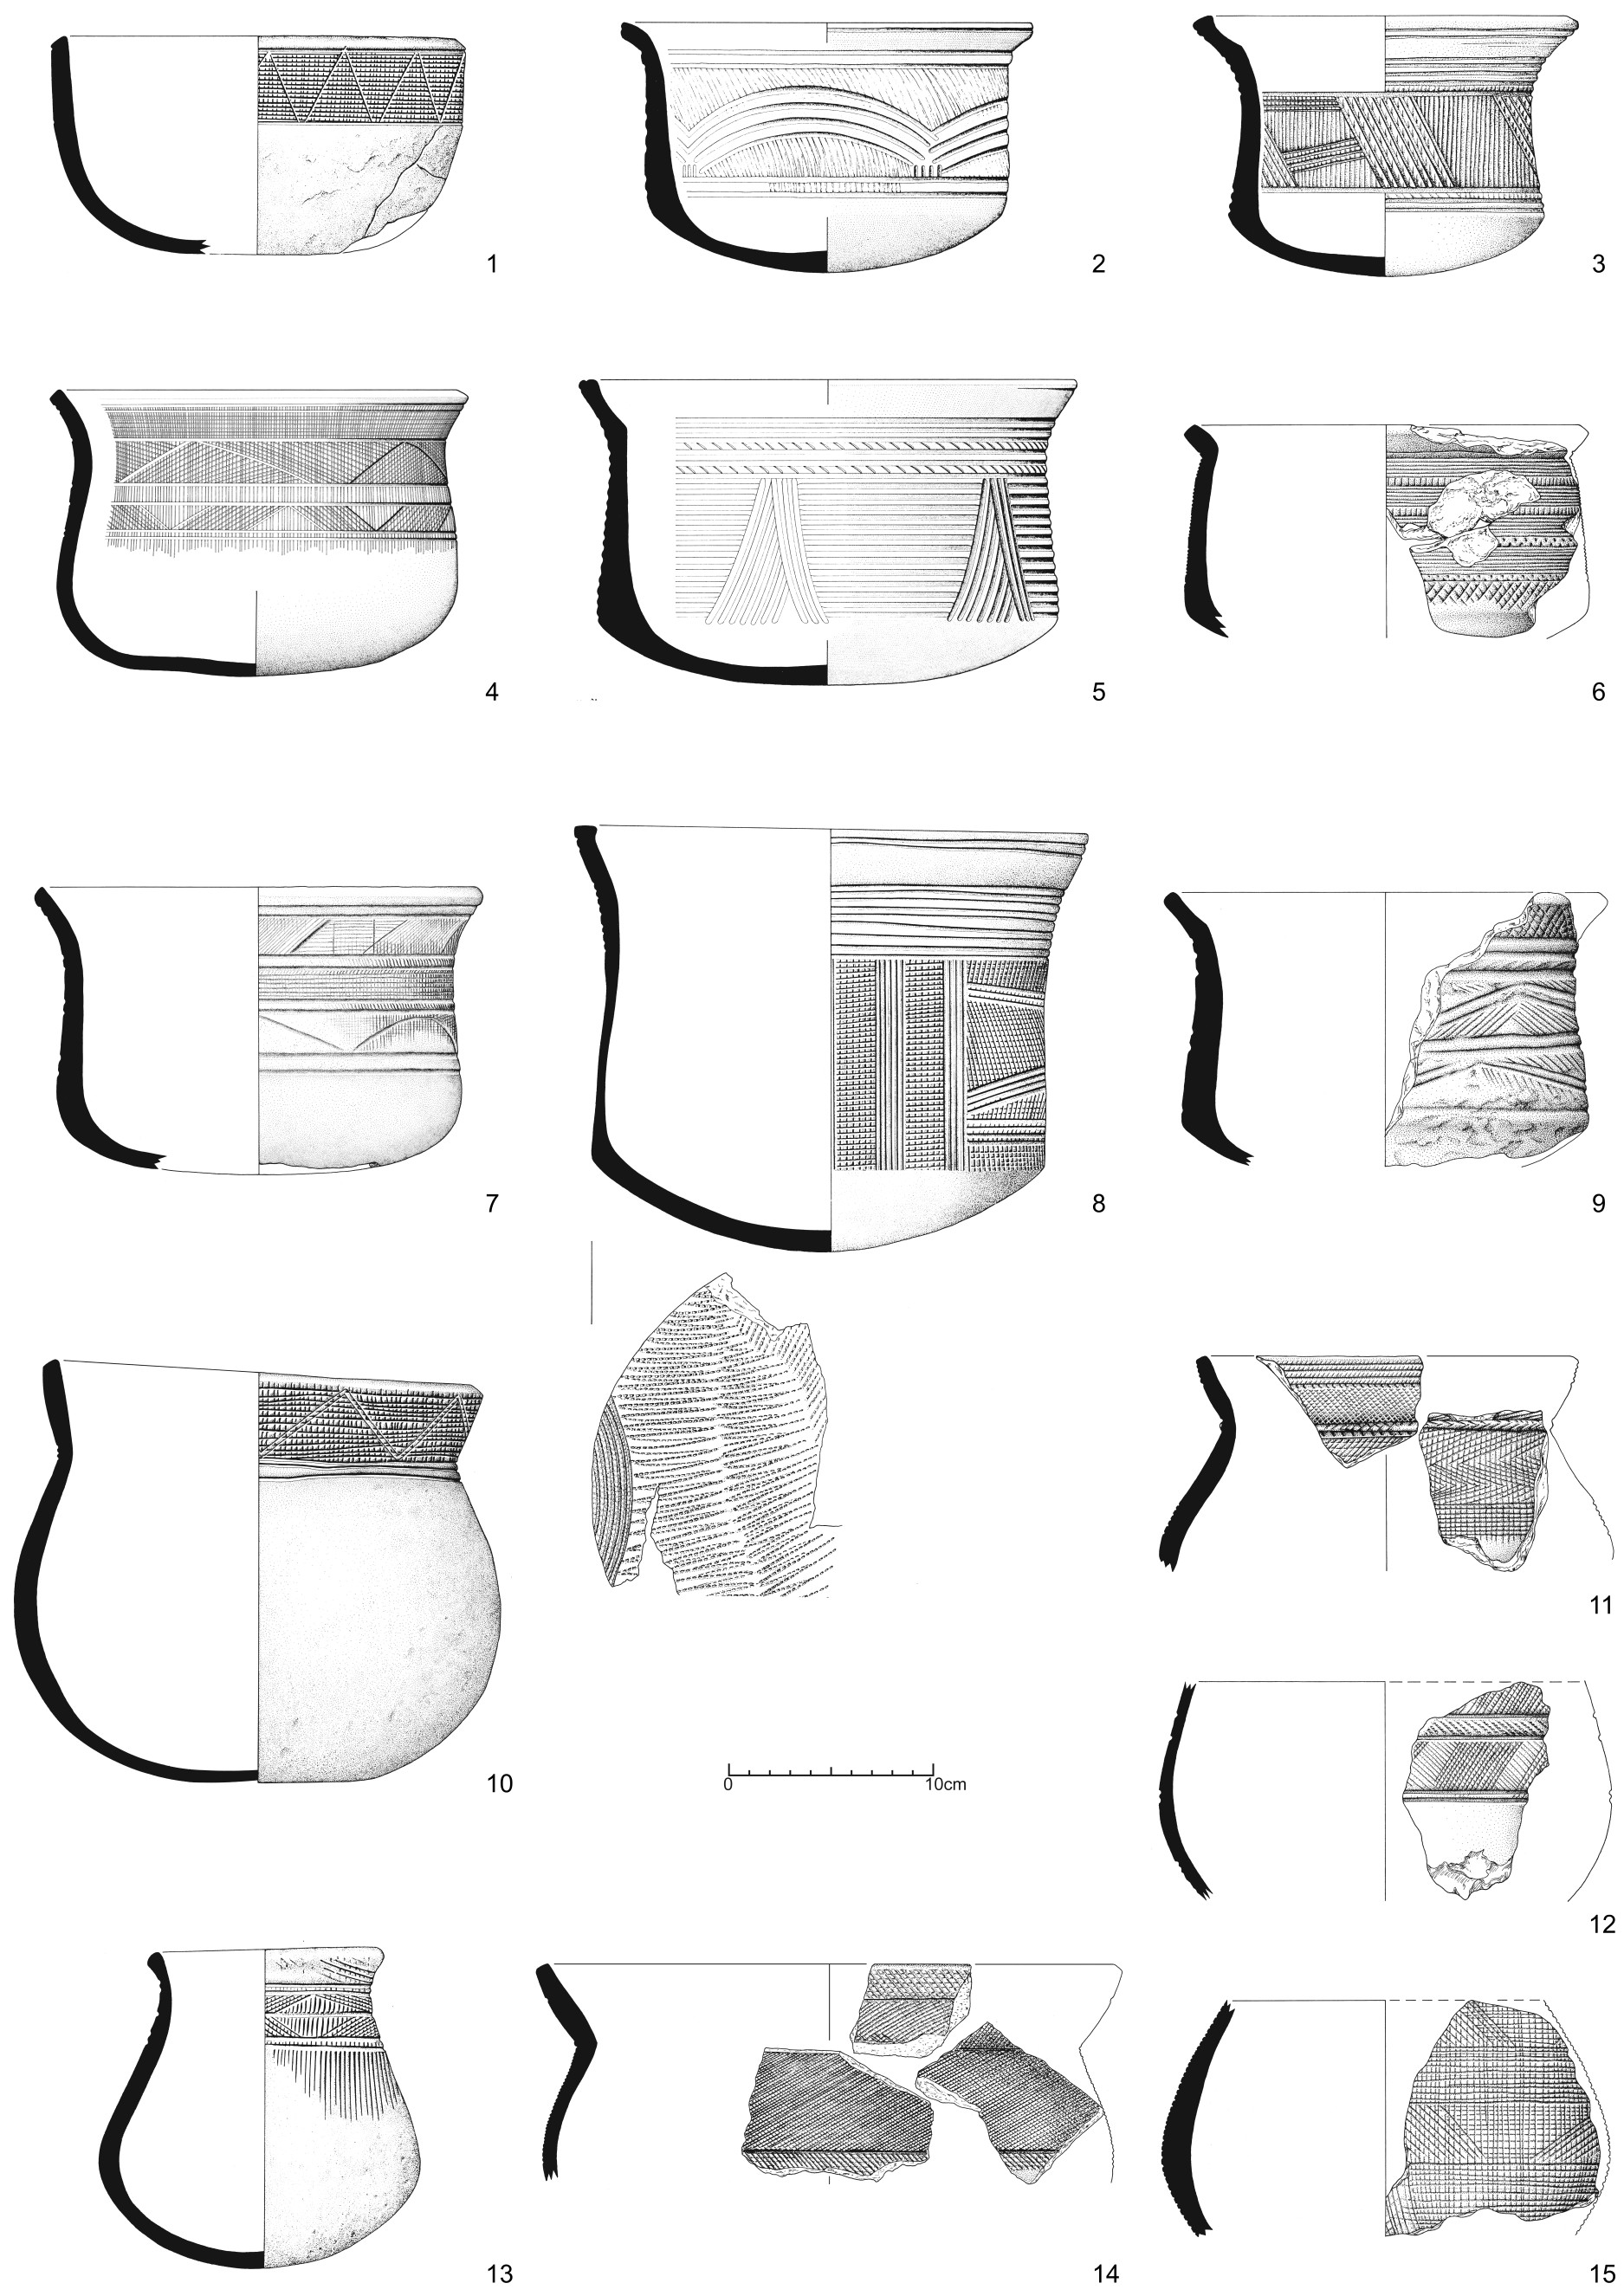
\includegraphics[width=\textwidth]{fig/PKM-Typen.pdf}
	\caption{Pikunda-Munda-Gruppe: Typvertreter.\\1:~Taf.~92.5; 2:~Taf.~91.1; 3:~Taf.~50.1; 4:~Taf.~92.7; 5:~Taf.~91.5; 6:~Taf.~32.1; 7:~Taf.~91.7; 8:~Taf.~44.3; 9:~Taf.~94.1; 10:~Taf.~93.3; 11:~Taf.~51.1; 12:~Taf.~46.20; 13:~Taf.~92.8; 14:~Taf.~45.1; 15:~Taf.~51.3.}
	\label{fig:PIKMUN_TypVertreter}
\end{figure*}

\paragraph{Formen}\hspace{-.5em}|\hspace{.5em}%
Das bestimmende Charakteristikum der Pikunda-Munda-Gruppe sind hohe Schalen mit Bauch"-umbruch oder -knick, ausbiegendem Rand und rundem Boden vom Typ E3 sowie F3 (Abb. \ref{fig:PIKMUN_TypVertreter}.2--9). Daneben sind nur wenige weitere Gefäßformen bekannt (Abb.~\ref{fig:PIKMUN_TypVertreter}.1,10--15). Die beiden charakteristischen Schalenformen machen jeweils 40--43\,\% aller sicher zu bestimmenden Gefäßformen der Pikunda-Munda-Gruppe aus. Gefäße mit geschweifter Wandung, die keinen dezidiert ausgearbeiteten Halsbereich aufweisen, ließen sich bei 10\,\% aller GE der Pikunda-Munda-Gruppe nachweisen (Typ~E1; Abb.~\ref{fig:PIKMUN_TypVertreter}.10--12,14--15).\vspace{1em}

\begin{figure*}[tb]
	\noindent\begin{minipage}[b]{\columnwidth}
		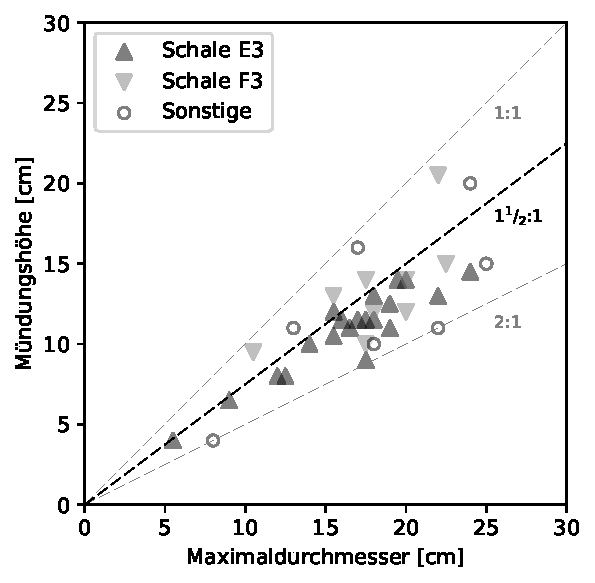
\includegraphics[width=\columnwidth]{fig/PKM_Proportionen.pdf}
		\captionof{figure}{Pikunda-Munda-Gruppe: Proportionen der Gefäße.\label{fig:PIKMUN_Proportionen}}\vspace{1em}
		\captionof{figure}{Pikunda-Munda-Gruppe: Kalibierung der \textsuperscript{14}C-Datierungen für die Gruppen I und II (Siehe Anlage~2).\label{fig:PIKMUN_14C}}\vspace{1em}
	\end{minipage}\hfill
	\noindent\begin{minipage}[b]{\columnwidth}
	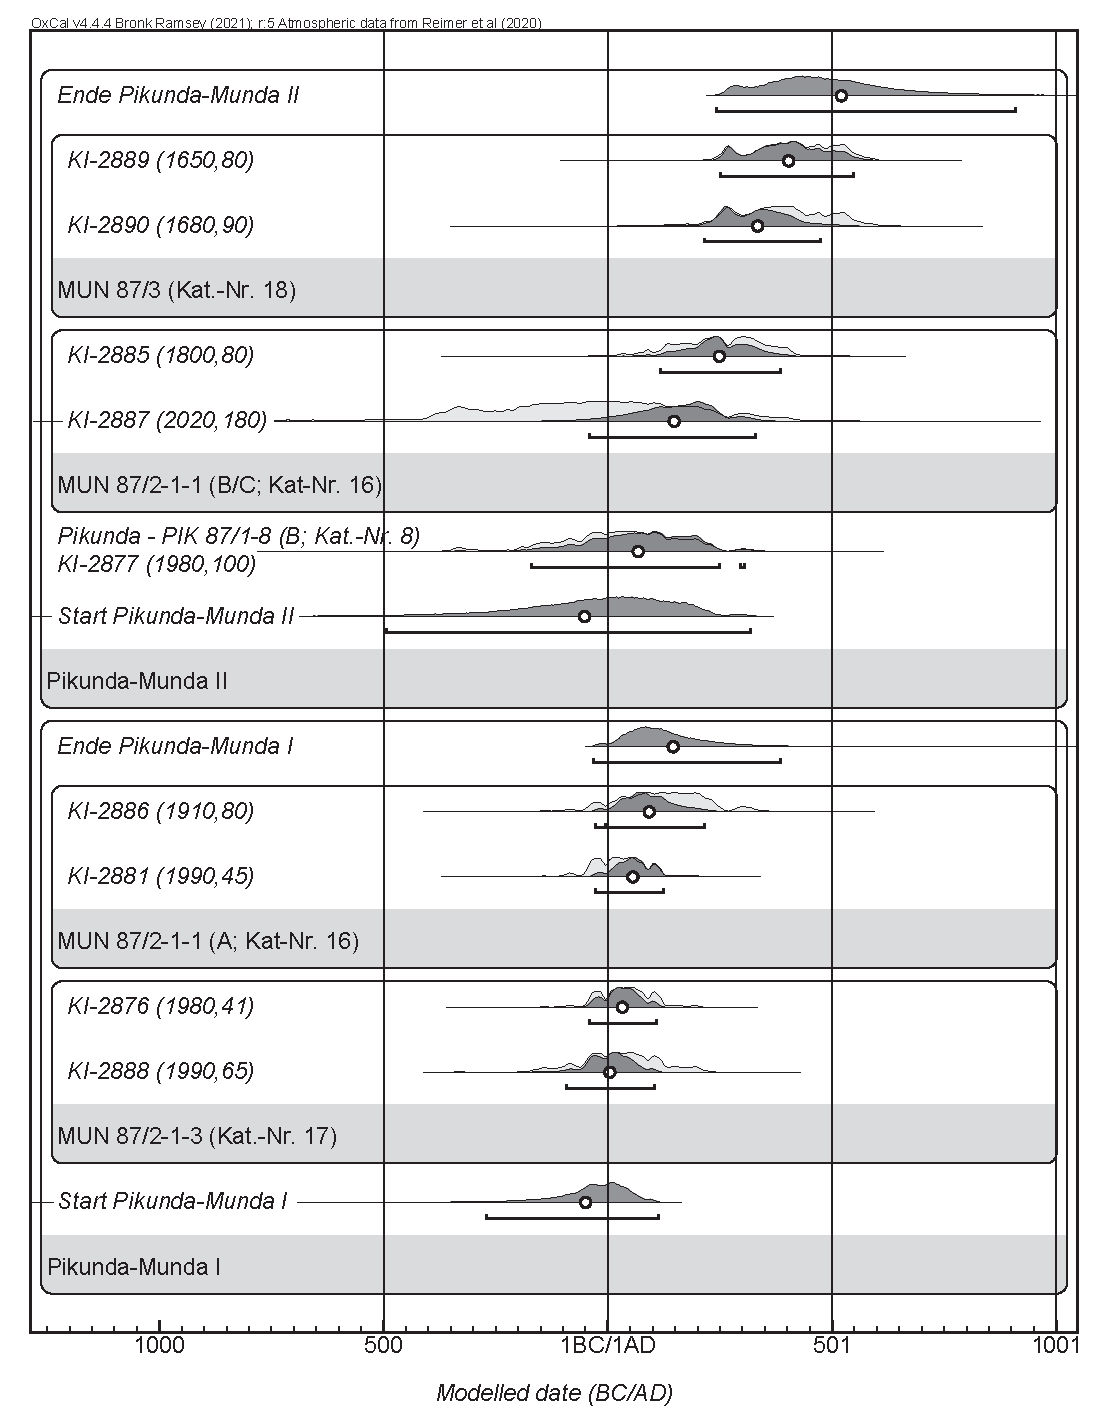
\includegraphics[width=\columnwidth]{fig/PKM_14C.pdf}
	\end{minipage}
\end{figure*}

Schalenförmige Gefäße mit konvexer Wandung (Typ~I; Abb.~\ref{fig:PIKMUN_TypVertreter}.1) sowie hohe Gefäße mit ausgeprägtem Halsbereich (Typ~B; Abb.~\ref{fig:PIKMUN_TypVertreter}.13) ließen sich lediglich als Einzelfunde beobachten. Die Schalen sind im Schnitt etwa anderthalb mal so breit wie hoch, wobei die Schalen des Typs E3 tendenziell etwas flacher als jene des Typs F3 sind (Abb.~\ref{fig:PIKMUN_Proportionen}). Der Mündungsdurchmesser der Schalen vom Typ E3 liegt zwischen 6 und 31\,cm, während er bei den Schalen vom Typ F3 zwischen 11 und 31\,cm schwankt. Die Höhe der Schalen variiert zwischen 4 und 14,5\,cm (Typ~E3) beziehungsweise 9,5 und 20,5\,cm (Typ~F3). Während die Ränder deutlich über den minimalen Gefäßdurchmesser hinausragen, im Schnitt um knapp 16\,\%, ist der maximale Durchmesser im Bereich der Gefäßwandung, der direkt zum Gefäßboden umleitet, nur etwa 5--10\,\% größer als der Minimaldurchmesser.

Mit Bezug auf die Ausgestaltung der Randlippen ließen sich im Material der Pikunda-Munda-Gruppe zu in etwa gleichen Anteilen runde (M1; 32\,\%; Abb. \ref{fig:PIKMUN_TypVertreter}.13), gerade (M3; 32\,\%; Abb. \ref{fig:PIKMUN_TypVertreter}.5,8) sowie schräg nach außen (M5; 27\,\%; Abb.~\ref{fig:PIKMUN_TypVertreter}.1,3--4,6--7,9--11) abgestrichene Mündungsabschlüsse beobachten. Gerillte Randlippen (M4) fanden sich nur bei 3\,\% der Stücke (Abb.~\ref{fig:PIKMUN_TypVertreter}.2). Die Ränder selbst sind regelhaft ausbiegend. Zu etwa gleichen Anteilen lassen sich gerade (B1; 29\,\%; Abb.~\ref{fig:PIKMUN_TypVertreter}.6,8--11) sowie konkav (B2; 30\,\%; Abb.~\ref{fig:PIKMUN_TypVertreter}.2,4,7,13) und konvex (B3; 26\,\%; Abb.~\ref{fig:PIKMUN_TypVertreter}.3,5) ausbiegende Ränder beobachten. Nur selten sind gerade aufsteigende Ränder zu beobachten (A1; 9\,\%, Abb.~\ref{fig:PIKMUN_TypVertreter}.1). Die Böden sind mit wenigen Ausnahmen, die allesamt eher als unbeabsichtigte Einzelfälle denn als beabsichtigte Produkte des Töpfereiprozesses angesehen werden können, rund ausgeführt (Abb.~\ref{fig:PIKMUN_TypVertreter}.1, 10). Der Bodentyp B1 findet sich bei 86\,\% der 64~GE, bei denen die Form des Bodens aufgenommen werden konnte.

\paragraph{Verzierungen}\hspace{-.5em}|\hspace{.5em}%
Pikunda-Munda-Keramik zeichnet sich durch eine im Grundsatz sehr klare und homogene Verzierungspraxis aus. Während die Gefäßunterteile und runden Böden nur sehr selten verziert sind, in einigen Fällen lässt sich Kamm-Wiegeband beobachten (Tab.~\ref{tab:Verzierungselemente}: 04.2; 2\,\%; Abb.~\ref{fig:PIKMUN_TypVertreter}.8), weisen die Oberteile eine vornehmlich durch horizontale Bänder gegliederte, umfangreiche Verzierung auf (Anlage~4\subref{fig:PIKMUN_Verz}). Zusammengenommen machen Rillen (Tab.~\ref{tab:Verzierungselemente}: 01) und Riefen (Tab.~\ref{tab:Verzierungselemente}: 02) 82\,\% aller an GE der Pikunda-Munda-Gruppe beobachteten Verzierungselementen aus. Horizontale Rillen (Tab.~\ref{tab:Verzierungselemente}: 02.1) finden sich vornehmlich außen auf dem Rand sowie Bauch der Gefäße machen 34\,\% aller Verzierungen aus, gefolgt von dem aus sich überkreuzenden Rillen aufgebauten Schachbrettmuster (24\,\%; Tab.~\ref{tab:Verzierungselemente}: 01.1--4). Neben diesen regelhaft zu beobachtenden Verzierungselementen fällt die Nutzung von horizontalen Reihen aus kleinen, häufig diagonal gesetzten Eindrücken auf (Tab.~\ref{tab:Verzierungselemente}: 04.12; 6\,\%). Grundsätzlich sind fast alle im Katalog der Verzierungselemente aufgenommen Variationen von Rillen (Tab.~\ref{tab:Verzierungselemente}: 01) und Riefen (Tab.~\ref{tab:Verzierungselemente}: 02) auf den GE der Pikunda-Munda-Gruppe vertreten. Durch die Verzierung der GE wird insbesondere der Rand sowie der Gefäßbauch betont. Auffällig ist dabei eine Tendenz zu horizontalen Bändern und flächigen Mustern sowie eine durch vertikal gesetzte Verzierungselemente erzeugte, metopenartige Strukturierung der Verzierung. 

\begin{table*}[tb!]
	\centering{\footnotesize \begin{sftabular}{@{}lccc|ccccccc@{}}
			\toprule
			\multirow{2}{*}{} & \multicolumn{2}{c}{\textbf{PKM}} & \multirow{2}{*}{\textbf{LKW 186}} & \multirow{2}{*}{\textbf{IMB}} & \multirow{2}{*}{\textbf{BON}} & \multirow{2}{*}{\textbf{ING}} & \multirow{2}{*}{\textbf{LOK}} & \multirow{2}{*}{\textbf{BKE}} & \multirow{2}{*}{\textbf{LUS}} & \multirow{2}{*}{\textbf{LNG}} \\
			& \multicolumn{1}{c}{\textbf{I}} & \multicolumn{1}{c}{\textbf{II}} &  & & & & & &  \\
			\midrule
			Topf mit Schulterabsatz (Typ~C) &  &  & $\circ$ & $\bullet$ & $\bullet$ & $\circ$ &  &  &  &  \\
			Schale mit Bauchknick (Typ E3 \& F3) & $\circ$ & $\bullet$ & & &  &  &  & $\circ$ &  &  \\
			Rundbodig (B1--3) & $\bullet$ & $\bullet$ &  &  &  &  &  & $\bullet$ & &  \\
			Flachbodig (B1--14) & $\circ$ &  & $\bullet$  & $\bullet$  & $\bullet$ & $\bullet$ & $\bullet$ & $\bullet$ & $\bullet$ & $\bullet$ \\
			Kamm-Wiegeband (Tab.~\ref{tab:Verzierungselemente}: 04.1) &  & $\bullet$ &  & $\bullet$ & $\bullet$ & $\bullet$ &  & & & \\
			\textit{Schachbrett}-Muster (Tab.~\ref{tab:Verzierungselemente}: 01.1--4) &  & $\bullet$ &  &  &  &  & $\bullet$ & &  & $\bullet$ \\
			\textit{Fabric} 1--2 & $\bullet$ & $\bullet$ & $\circ$ & $\circ$  & $\circ$  & $\circ$  & $\bullet$ & $\circ$ & $\circ$ & $\circ$ \\
			\bottomrule
	\end{sftabular}}
	\caption{Pikunda-Munda-Gruppe: Gegenüberstellung von formalen Merkmalen und Verzierungspraxis der postulierten Untergruppen der Pikunda-Munda-Gruppe zum Inventar aus LKW~87/186 (Kat.-Nr.~19) sowie zeitgleichen Stilgruppen und der älteren Imbonga-Gruppe des Inneren Kongobeckens.\\$\bullet$ vorhanden, $\circ$ fraglich. \\ PKM: Pikunda-Munda, LKW 186: Inventar des Komplexes LKW~87/186 (Kat.-Nr.~19), IMB: Imbonga (\textsc{Wotzka} 1995: 59--68), BON: Bonkake (ebd. 68--73),\\ING: Ingende (ebd. 73--78), LOK: Lokondola (ebd. 84--89), BKL: Bokele (ebd. 100--104), LUS: Lusako (ebd. 104--107), LNG: Lingonda (ebd. 108--115).}
	\label{tab:PIKMUN_Vgl}
\end{table*}

\paragraph{Datierung}\hspace{-.5em}|\hspace{.5em}%
Mit Keramik des Pikunda-Munda-Stils sind neun Radiokohlenstoffdatierungen assoziiert (Tab.~\ref{tab:14Cdatings}). Diese stammen ausnahmslos aus den für die Beschreibung der Stilgruppe zentralen Ausgrabungen in Pikunda am \mbox{Sangha} (Fpl.~255) und Munda am \mbox{Likwala}-\mbox{aux}-\mbox{Herbes} (Fpl.~304). Die Grabung MUN~87/2-1-1 (Kat-Nr.~16) in Munda (Fpl.~304) erbrachte einen stratifizierten Befund, der eine Differenzierung des keramischen Materials der Pikunda-Munda-Gruppe in zwei Unterstile andeutet. Zwei, klar durch eine verziegelte Lehmwanne voneinander getrennte Grubenverfüllungen erbrachten jeweils homogene Inventare. Beide fallen grundsätzlich in das Spektrum der Pikunda-Munda-Gruppe, da die charakteristischen Schalenformen das bestimmende Merkmal sind, weisen jedoch auch Abweichungen zueinander auf. In der stratigrafisch älteren Verfüllung A (siehe Kat-Nr.~16) fanden sich ausnahmslos Pikunda-Munda-Schalen mit einem runden, geschweiften Umbruch des Gefäßbauches (Typ~E3; Taf.~91.6--8). Diese entsprechenden Schalen der Untergruppe I der Pikunda-Munda-Gruppe zeichnen sich durch eine Verzierung aus, die fast ausschließlich aus flachen Rillen bestehenden horizontalen Bändern (Tab.~\ref{tab:Verzierungselemente}: 02.1) sowie Schachbrettmustern (Tab.~\ref{tab:Verzierungselemente}: 01.1) auf den Rändern und Bauchbereichen der Gefäße besteht. Ein diesem morphologisch wie ornamental entsprechendes Inventar fand sich in der nur 0,35\,m nördlich anschließenden Grube MUN~87/2-1-3 (Kat.-Nr.~17). Im Unterschied zu den Gefäßen des unteren Verfüllungsbereiches A in MUN~87/2-1-1 erbrachte der obere Verfüllungsbereich C ein Inventar, welches größtenteils aus Schalen mit einem deutlich ausgeprägten Bauchknick besteht (Typ~F3; Taf.~91.1--5). Dieses ist repräsentativ für die Untergruppe II des Pikunda-Munda-Stils. Die Schalen weisen eine leicht andere Ornamentik auf, die auf tieferen Rillen und flächigem Wiegeband mit Klinge oder Kamm basiert (Tab.~\ref{tab:Verzierungselemente}: 04.1--2). Die durch die Grabung PIK~87/1 (Kat.-Nr.~8) in Pikunda am \mbox{Sangha} (Fpl.~255) erschlossene Grube B1/B2 erbrachte ebenfalls ausschließlich Pikunda-Munda-Schalen mit einem Profilknick vom Typ F3. Die aus diesen Beobachtungen ableitbaren Untergruppen der Pikunda-Munda-Gruppe weisen trennende wie verbindende Merkmale auf (Tab.~\ref{tab:PIKMUN_Vgl}). Die Schalenformen vom Typ E3 mit ihrem auffällig abgerundeten Bauchumbruch (Abb.~\ref{fig:PIKMUN_TypVertreter}.4,7) stehen dabei den Schalen vom Typ F3 gegenüber, die einen deutlichen und teilweise scharfen Bauchknick aufweisen (Abb.~\ref{fig:PIKMUN_TypVertreter}.3--4,5--6,8--9).

\begin{figure*}[p]
	\centering
	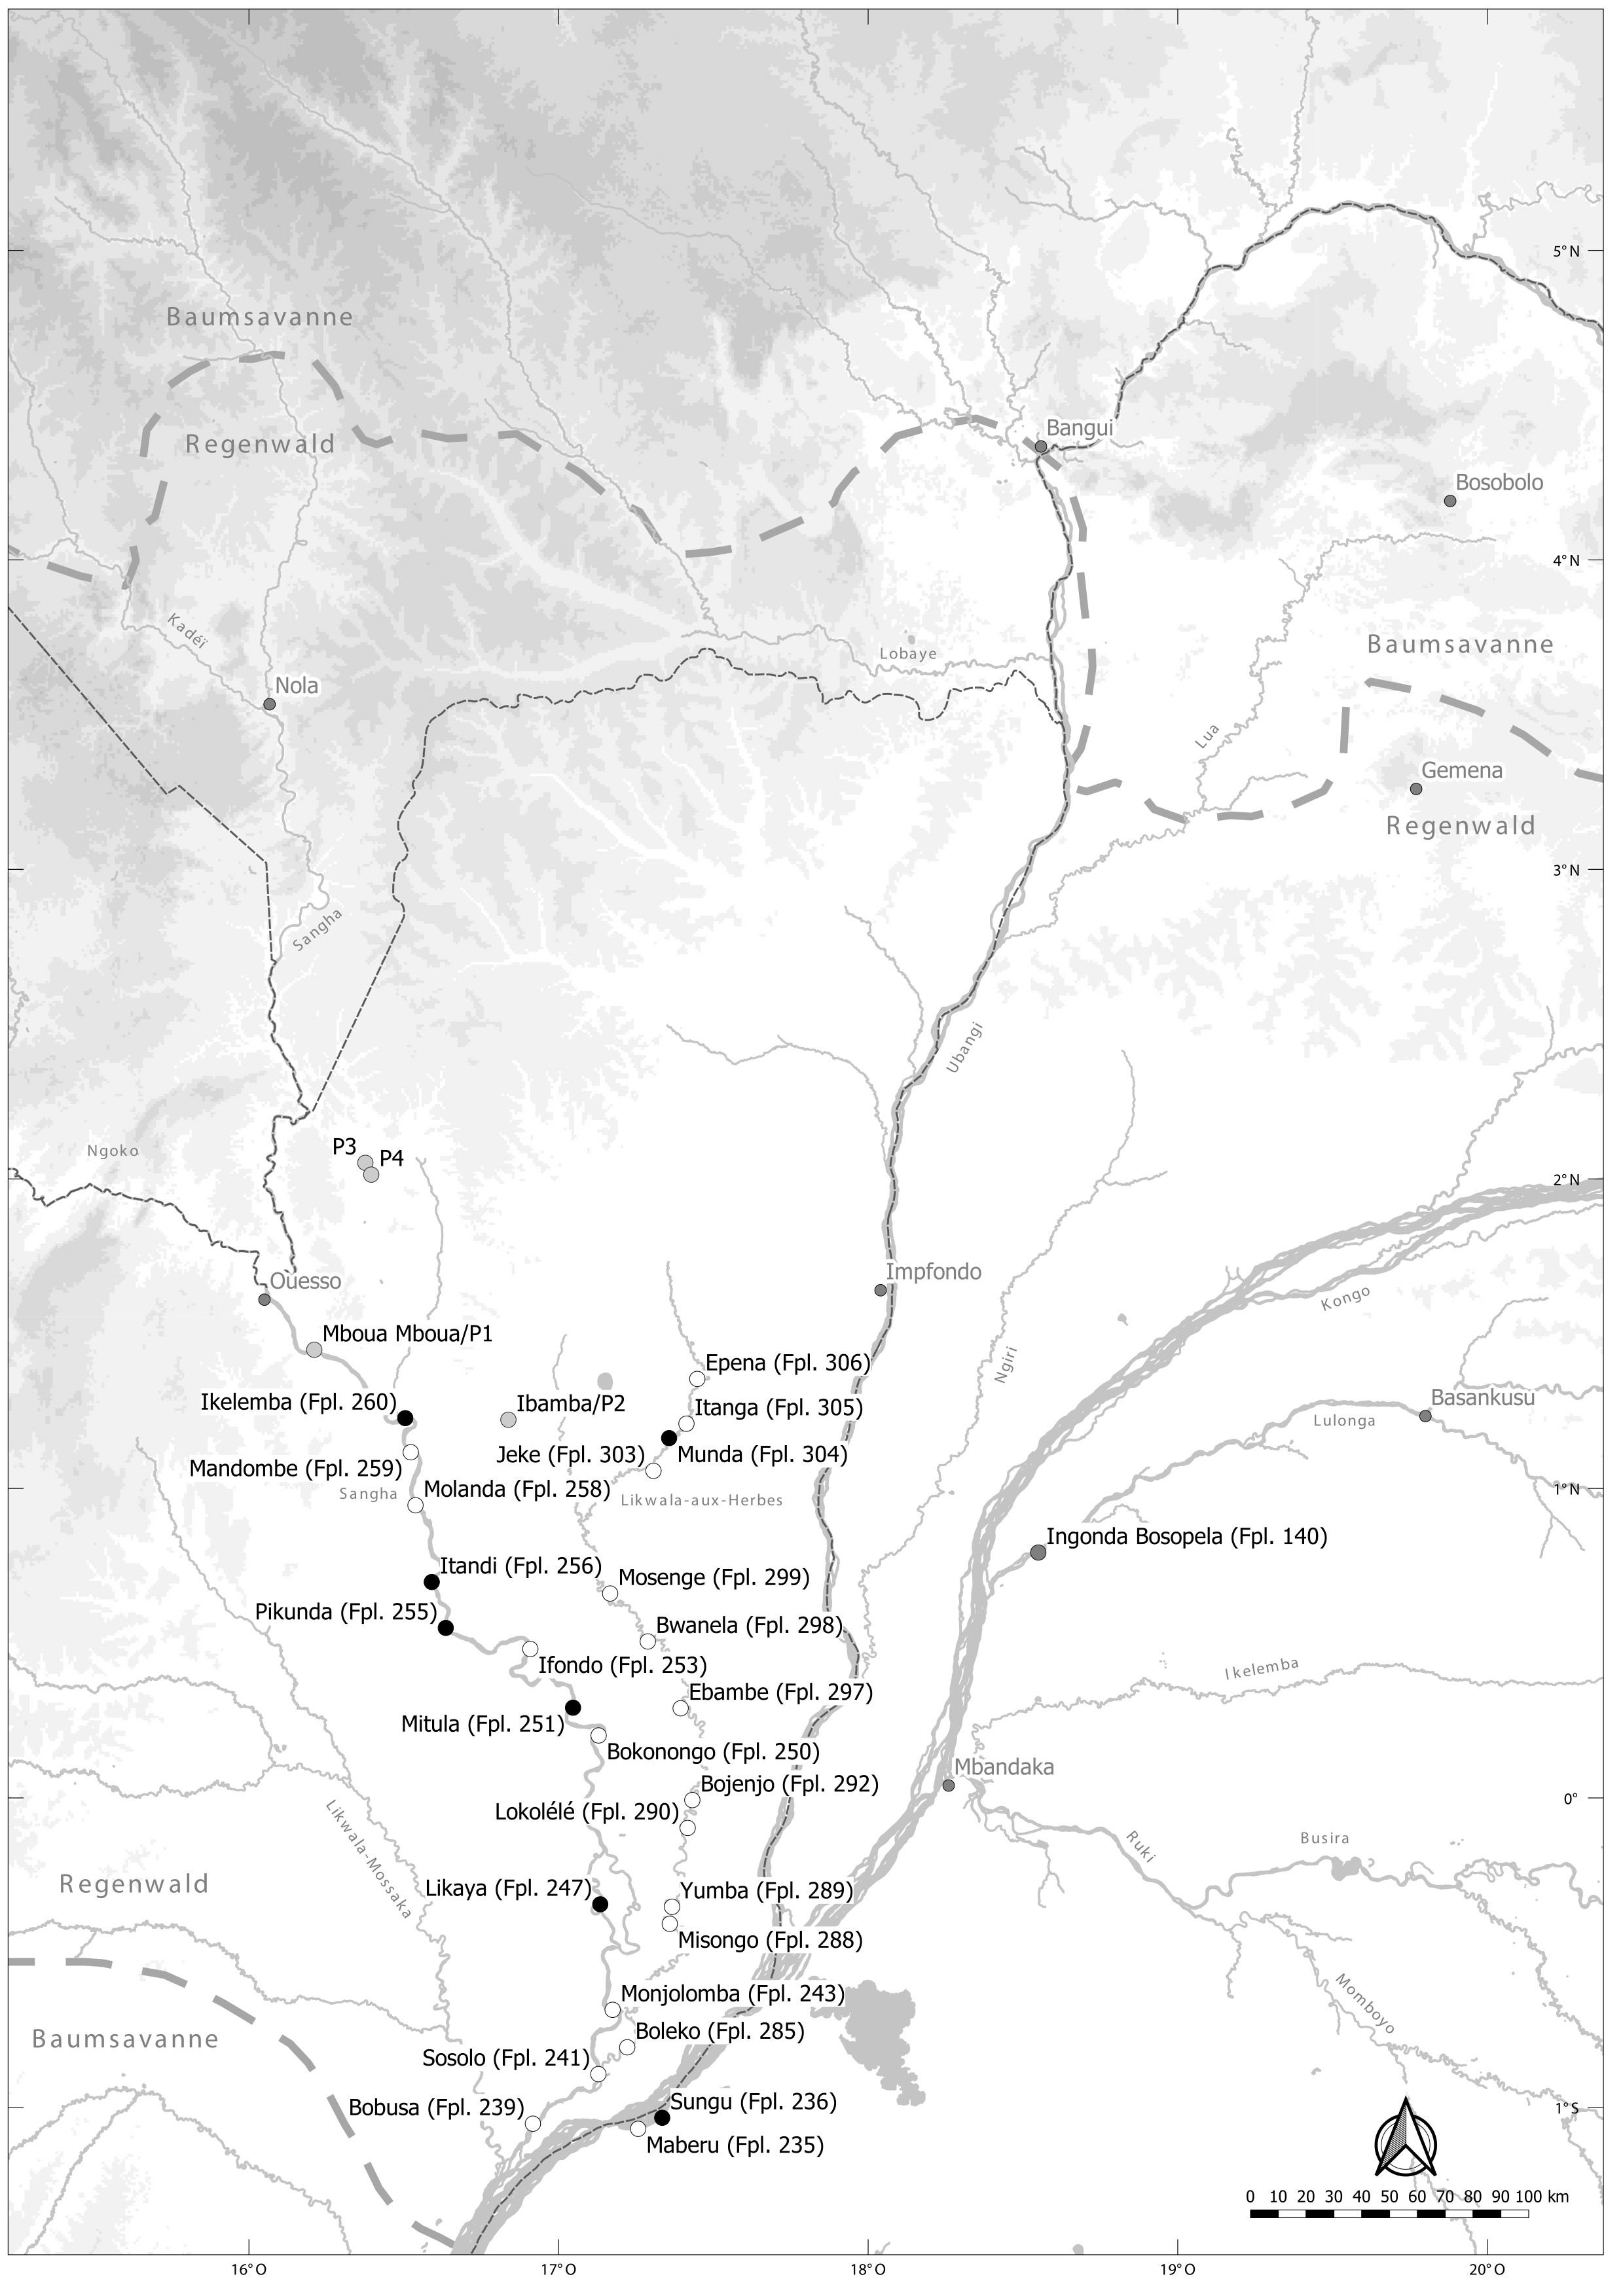
\includegraphics[width=\textwidth]{fig/PKM_Verbreitung.pdf}
	\caption{Pikunda-Munda-Gruppe: Verbreitung \parencites[grau nach][119 Anm.~4, 531 Taf.~97.5]{Wotzka.1995}[114 Abb.~42]{Gillet.2013}.}
	\label{fig:PIKMUN_Verbreitung}
\end{figure*}

Der Beginn des Pikunda-Munda-Stils kann auf Basis der vorliegenden Datierungen in das 2.--1.~Jh. v.~Chr. datiert werden (Abb.~\ref{fig:PIKMUN_14C}), wenn die Datierung KI-2887 (Tab.~\ref{tab:MUN87-211_14C-Daten}; Anlage 2) ausgelassen wird, das diese einen besonders hohen Standardfehler aufweist. Die jüngsten Radiokohlenstoffdatierungen für Pikunda-Munda-Keramik stammen aus dem Befund MUN~87/3 in Munda am \mbox{Likwala}-\mbox{aux}-\mbox{Herbes} und fallen in das 2.-6.~Jh. n.~Chr. (Abb.~\ref{fig:PIKMUN_14C}: KI-2889, KI-2890).\footnote{Die Keramik dieses Befundes spiegelt mit einer Schale vom Typ F3 (Abb.~\ref{fig:PIKMUN_TypVertreter}.9) die formalen Charakteristika der Untergruppe II wider.} Bereits \textsc{Wotzka} (1995: 107 Anm.~4) hat auf den Umstand hingewiesen, dass sich gewisse Merkmale der Pikunda-Munda-Keramik auch bei keramischen Stilgruppen des Inneren Kongobeckens beobachten lassen (Tab.~\ref{tab:PIKMUN_Vgl}).\footnote{Der Pikunda-Munda-Gruppe auf Merkmalsebene nahestehende Gefäße fanden sich im Zusammenhang mit Feldarbeit an der Fundstelle Yatou in Kamerun an der Mündung des Sanaga-Flusses (siehe Kap.~\ref{sec:Kamerun}). Die beiden aus dem Befund YAT~99/1 vorliegenden Radiokohlenstoffdatierungen decken das 1.~Jh. v.~Chr. bis 1.~Jh. n.~Chr. (KIA-12942) sowie das 7.--9.~Jh. n.~Chr. (KIA-12941) ab. Gerade die ältere der beiden Datierungen lässt sich leicht mit dem hier postulierten Alter für die Pikunda-Munda-Gruppe in Einklang bringen. Eine detaillierte Auswertung der Befunde und Funde aus Yatou steht gegenwärtig aus (Kap.~\ref{sec:Kamerun}).} Während die für den Pikunda-Munda-Stil charakteristischen Schalen keine Entsprechung im Fundgut des Inneren Kongobeckens finden, so ist Kamm-Wiegeband-Dekor ein starkes Merkmal der ältesten Stile Imbonga, Bonkake und Ingende (ebd. 59--78). Auch ein aus überkreuzenden, feinen Ritzlinien bestehendes Dekor findet sich in zeitgleichen Stilen, allen voran der Lokondola-Gruppe.\footnote{Eine Scherbe dieses Stils fand sich auch in der älteren, in Pikunda erfassten Grube (Kat.-Nr.~8).} Zusammenfassend lässt sich festhalten, dass der Pikunda-Munda-Stil stilistisch einige lose Anbindungen an die zeitgleichen Stilgruppen des Inneren Kongobeckens aufweist, jedoch mit Blick auf die Keramiktechnologie nicht von der weiter östlich gefunden Keramik unterscheidbar ist. Zusammenfassend kann die Pikunda-Munda-Keramik gegenwärtig mit hinreichender Sicherheit in das 2.--1.~Jh. v.~Chr. bis 5.--6.~Jh. n.~Chr. datiert werden.

\paragraph{Verbreitung}\hspace{-.5em}|\hspace{.5em}%
Die Verbreitung der Pikunda-Munda-Keramik (Abb.~\ref{fig:PIKMUN_Verbreitung}) beschränkt sich auf die Flussläufe des \mbox{Sangha} und \mbox{Likwala}-\mbox{aux}-\mbox{Herbes} von deren Mündung in den Kongo bis Ikelemba am \mbox{Sangha} (Fpl.~260) beziehungsweise Epena am \mbox{Likwala}-\mbox{aux}-\mbox{Herbes} (Fpl.~306).\footnote{Erst im Zuge der Feldarbeiten der Arbeitsgruppe um Richard Oslisly wurde die Fundstelle Pikunda (Fpl.~255) in den frühen 2010er Jahren wieder aufgesucht \parencite[211 Abb.~1, 212\,f. Tab.~1 Nr.~25--26]{MorinRivat.2014}.} Material des Pikunda-Munda-Stils fand sich auch in Maberu (Fpl.~235) und Sungu (Fpl.~236) am Kongo, etwa 50\,km nordöstlich der Mündung des \mbox{Sangha}. Das Verbreitungsgebiet reicht folglich etwa 250\,km in Nord--Süd- und etwa 110\,km in Ost--West-Richtung.

Innerhalb der Komplexe aus Oberflächenabsammlungen war eine sichere Ansprache von Scherben des Pikunda-Munda-Stils aufgrund starker Fragmentierung und hoher Erosion der Oberflächen selten möglich. Zudem erschwerte die teils recht einfache Rillen- und Riefenverzierung (Tab.~\ref{tab:Verzierungselemente}: 01--02) die sichere Ansprache kleinerer Stücke. Daraus resultiert, dass große Teile der aus Oberflächenkomplexen stammenden Stücke lediglich unter Vorbehalt dem Pikunda-Munda-Stil zugeordnet werden konnten. Diese Unsicherheiten spiegeln sich auch im Verbreitungsgebiet der Pikunda-Munda-Gruppe wider (Abb.~\ref{fig:PIKMUN_Verbreitung}). Entlang des \mbox{Likwala}-\mbox{aux}-\mbox{Herbes} sowie im \mbox{Sangha}-Mündungsgebiet lagen häufig keine ausreichenden Merkmale für eine sichere Ansprache vor, und manche Scherben konnten nur unter Vorbehalt angesprochen werden.

Aus dem von \textsc{Wotzka} (1995: 119 Anm. 4, 531 Taf.~97.5) bearbeiteten Inneren Kongobecken liegt ein, im Zuge von Surveys gefundenes Gefäß aus Ingonda Bosopela am unteren Lulonga (Fpl. 140) vor.\footnote{Dabei handelt es sich um das Fragment einer Schale mit ausbiegendem Rand, gerader oberer Wandung und einem auffälligen, runden Bauchumbruch, das dem Gefäßtyp E3 zugeordnet werden kann. Die Verzierung dieses Stücks besteht aus Riefen, die ein aus feinen, vertikalen Rillen bestehendes Band einrahmen, das zudem von girlandenartigen Rillen überlagert wird (Tab.~\ref{tab:Verzierungselemente}: 02.1, 02.2, 02.5). Der Randabschluss weist feine, diagonal sitzende Rillen oder Eindrücke auf \parencite[Tab.~\ref{tab:Verzierungselemente}: 02.3 oder 04.12; 119 Anm. 4, 531 Taf.~97.5]{Wotzka.1995}.} Des Weiteren sind potenzielle Scherben der Pikunda-Munda-Gruppe an vier Plätzen belegt, die im Rahmen ökologischer Untersuchungen im Norden der Republik Kongo erschlossen wurden \parencite[114 Abb.~42; Abb.~\ref{fig:PIKMUN_Verbreitung}]{Gillet.2013}. Die Fundstellen zeichnen sich neben den keramischen Funden durch bei Bohrungen erfasste Holzkohlekonzentrationen aus (ebd. 94 Tab.~14). Da die Ansprache lediglich anhand der veröffentlichten Fotografien erfolgte, kann eine Zuweisung nur unter starken Vorbehalten postuliert werden. Akzeptierte man diese Fundpunkte jedoch, so würde sich das Verbreitungsgebiet der Pikunda-Munda-Gruppe um etwa 50\,km nach Norden ausweiten, auf eine Ausdehnung von etwa 300\,km in Nord--Süd-Richtung.

\subsubsection{Bokonongo-Gruppe}\label{sec:BOG-Gr}

An fünf Fundstellen entlang des unteren \mbox{Sangha} sowie an zweien am Kongo (Abb.~\ref{fig:BOG_Verbreitung}) wurden bei Surveys sehr charakteristische keramische Formen gefunden, die mit einer Ausnahme\footnote{Lediglich in Sosolo an der Mündung des \mbox{Sangha} (Fpl.~241) wurden zehn GE gefunden, die der Bokonogo-Gruppe zugeweisen werden können.} fast ausschließlich als Einzelfunde an den jeweiligen Plätzen auftraten. Die nach dem eponymen Fundort Bokono\-ngo am mittleren \mbox{Sangha} (Fpl.~250) benannte Stilgruppe zeichnet sich durch eine spezifische Ausgestaltung des Gefäßrandes bei einer der beiden beobachteten Gefäßformen aus: kurze, konvex ausbiegende Ränder (B3.1), die häufig in einem geraden, zylindrischen Mündungsabschluss enden (Abb.~\ref{fig:BOG-Typen}.1--4). Zudem umfasst das Formenspektrum der Bokonongo-Gruppe noch Schalen mit einbiegendem Rand (Abb.~\ref{fig:BOG-Typen}.5--9).

Insgesamt wurden 19~GE beobachtet, die der Stilgruppe zugerechnet werden können. Alle Stücke stammen aus Oberflächenabsammlungen, wodurch die mögliche Vergesellschaftung dieser mit anderen Formen sowie ihre chronologische Einordnung stark eingeschränkt ist. Eine ähnlich spezifische Ausprägung der Randgestaltung findet sich bislang nur in der als Oveng-Gruppe geführten, früheisenzeitlichen Keramik aus Gabun \parencites[615--618]{Clist.20042005}[134 Abb. 15]{GonzalesRuibal.2012}[217--299]{SanchezElipe.2015}[351--355]{SanchezElipe.2016}. Lose erinnert sie aber auch an einige Ränder des Pikunda-Munda-Stils (Abb.~\ref{fig:PIKMUN_TypVertreter}.3, 5; Taf.~50.7). Die Bokonongo-Gruppe setzt sich aus drei vollständigen oder hinreichend erhaltenen Gefäßen (Abb.~\ref{fig:BOG-Typen}.3--4; Taf.~54.1) sowie 16 großen Randfragmenten zusammen. In Anbetracht der spärlichen Datenlage kann die postulierte Zusammengehörigkeit der hier als Bokonongo-Stil systematisierten keramischen Formen lediglich als Provisorium angesehen werden.

\begin{figure*}[!tb]
	\centering
	\includegraphics[width=\textwidth]{fig/BOG-Typen.pdf}
	\caption{Bokonongo-Gruppe: Typvertreter im nordwestlichen Kongobecken.\\1:~Taf.~40.3; 2:~Taf.~35.9; 3:~Taf.~40.8; 4:~Taf.~51.11; 5: Taf.~29.3; 6: Taf.~36.1; 7: Taf.~36.4; 8: Taf.~29.5; 9: Taf.~32.13.}
	\label{fig:BOG-Typen}
\end{figure*}

\begin{figure*}[p]
	\centering
	\includegraphics[width=\textwidth]{fig/BOG_Verbreitung.pdf}
	\caption{Bokonongo-Gruppe: Verbreitung.}
	% \caption{Bokonongo-Gruppe: Verbreitung (Kreise) und Verbreitung der Oveng-Keramik in Gabun \parencites[Dreiecke, nach][615 Fig. 7-58]{Clist.20042005}{GonzalezRuibal.2011}{GonzalesRuibal.2012}.}
	\label{fig:BOG_Verbreitung}
\end{figure*}

\paragraph{Technologische Merkmale}\hspace{-.5em}|\hspace{.5em}%
Zwei Drittel aller der Bokonongo-Gruppe zugerechneten GE zeigen einen Scherben, praktisch ohne nichtplastische Partikel des \textit{Fabrics} 1 und 2 (Tab.~\ref{tab:Fabrics_Bilder}). Diese GE enthalten durchweg weniger als 10\,\% nichtplastische Partikel, die den Größenklassen \textit{very fine} bis \textit{medium} zugerechnet werden können. Wurden nichtplastische Partikel in den Scherben beobachtet, handelte es sich ausnahmslos um heterogenen Quarzsand. Das andere Drittel weist Fragmente von zerstoßener Keramik im Scherben auf und kann den \textit{Fabrics} 8 und 9 zugerechnet werden. Vertreter des \textit{Fabrics} 8, das sich durch Schamott und andere nichtplastische Partikel auszeichnet, waren ebenso häufig vertreten, wie Stücke, die ausschließlich Schamott enthalten und dem \textit{Fabric} 9 zuzurechnen sind. Während knapp die Hälfte der GE (48\,\%) eine Färbung aufweist, die auf die Nutzung eines weißbrennenden Tones hindeuten, zeigen zwei GE die Nutzung rotbrennender Tone an. Die Oberflächen der Stücke sind durchweg glatt (76\,\%) oder nur leicht rau.

\paragraph{Formen}\hspace{-.5em}|\hspace{.5em}%
Eine der beiden Grundformen der Bokonongo-Gruppe und das bestimmende Charakteristikum für die Beschreibung der Stilgruppe sind Gefäße mit geschweifter Wandung und dem eingangs beschriebenen konvex ausbiegendem Rand mit zylindrischem Abschluss vom Typ B3.1 (Abb.~\ref{fig:BOG-Typen}.1--4). Diese machen knapp die Hälfte aller der Bokonongo-Gruppe zugeordneten GE aus. Die andere Hälfte bilden schalenförmige Gefäße mit konvexer Wandung und einbiegendem Rand vom Typ H2 (Abb.~\ref{fig:BOG-Typen}.5--9). Während die Gefäßbäuche durchweg konvex sind, liegen keine GE vor, bei der der Boden erhalten wäre.

\paragraph{Verzierungen}\hspace{-.5em}|\hspace{.5em}%
Die Verzierungen der Bokonongo-Keramik sind, ähnlich wie jene der Pikunda-Munda-Keramik, von Rillen (Tab.~\ref{tab:Verzierungselemente}: 01) und Riefen (Tab.~\ref{tab:Verzierungselemente}: 02) bestimmt. Diese machen zusammen 78\,\% aller beobachteten Verzierungselemente aus (Anlage~4\subref{fig:BOG_Verz}). Bestimmendes Verzierungselement sind horizontale Rillen, die sich vornehmlich auf der Außenseite des Randes finden (Tab.~\ref{tab:Verzierungselemente}: 02.1; 39\,\%), gefolgt von vertikalen Rillen (Tab.~\ref{tab:Verzierungselemente}:02.2; 12\,\%) und horizontalen Reihen feiner Eindrücke (Tab.~\ref{tab:Verzierungselemente}: 04.12; 8\,\%). Ebenso häufig lassen sich aus Ritzlinien gebildete Schachbrettmuster beobachten (Tab.~\ref{tab:Verzierungselemente}: 01.1--4; 10\,\%). Die Verzierung wird vornehmlich in Form horizontaler Bänder unterhalb des Randes sowie am oberhalb des maximalen Durchmessers gelegenen Teil des Gefäßbauches aufgebracht (Abb.~\ref{fig:BOG-Typen}.1--3, 5--9). In seltenen Fällen lassen sich auch flächige Verzierungen des gesamten Gefäßkörpers beobachten (Abb.~\ref{fig:BOG-Typen}.4). Basierend auf den der Bokonongo-Gruppe zugewiesenen Stücken scheint das Unterteil der Gefäße, bis auf wenige Ausnahmen (Abb.~\ref{fig:BOG-Typen}.4), konsequent frei von Verzierungen zu sein. Regelhaft lässt sich auch die Überlagerung von Verzierungselementen beobachten (Abb.~\ref{fig:BOG-Typen}.3, 8--9).

\paragraph{Datierung}\hspace{-.5em}|\hspace{.5em}%
Für das ausschließlich aus Oberflächenabsammlungen bekannte Material der Bokonongo-Grup"-pe sind keine absoluten Daten bekannt. Keines der Stücke stammt aus einem ergraben Kontext. Eine direkte Datierung der Funde oder auf Basis die Vergesellschaftung mit anderem Fundgut ist daher nicht möglich.

Auffällig ist die eingangs erwähnte Parallele der Randgestaltung der geschlossenen Gefäße (Abb.~\ref{fig:BOG-Typen}.1--4) zu Material der Oveng-Gruppe in Gabun. Die Verbreitung dieser Keramik beschränkt sich auf das direkte Umland von Libreville im Westen Gabuns (ebd. 615 Fig.~7-58) sowie die der Küste vorgelagerte, zu Äquatorialguinea gehörende Insel Corisco \parencite[217--221]{SanchezElipe.2015}.\footnote{Siehe auch \textsc{González-Ruibal} u.a. (2011; 2012).} Die genannten Ränder lassen sich lose mit  jener von \textcite[559 Abb.~7-18.D]{Clist.20042005} als Var. \enquote{D} bezeichneten Ausprägung der Oveng-Keramik in Verbindung bringen. Das Inventar eines Verhüttungsbefundes von der durch sein früheisenzeitliches Gräberfeld bekannten Insel Corisco \parencite[134 Abb.~15]{GonzalesRuibal.2012} weist deutliche Parallelen zur Keramik der Bokonongo-Gruppe auf. Auch der Fokus der Verzierung auf den Bereich ausschließlich unterhalb des Randes und die Verwendung von diagonalen Kammeindrücken sowie Winkel- und Fischgrätmustern lässt sich bei GE der Bokonongo-Gruppe beobachten (Abb.~\ref{fig:BOG-Typen}.3,6--7). Die Keramik der Oveng-Gruppe wird in das 2.~Jh. v.~Chr. bis 5.~Jh. n.~Chr. datiert \parencite[555 Fig.~7-14]{Clist.20042005}.\footnote{Dieser Zeitraum entspricht grob der vorliegenden Datierung für den Pikunda-Munda-Stil (Abb.~\ref{fig:PIKMUN_14C}).} Für die Keramik der Bokonongo-Gruppe wird vorläufig ein entsprechender Datierungsansatz vorgeschlagen.

\paragraph{Verbreitung}\hspace{-.5em}|\hspace{.5em}%
Keramik des Bokonongo-Stils findet sich ausschließlich am unteren \mbox{Sangha} sowie im Bereich der \mbox{Sangha}-Mündung (Abb.~\ref{fig:BOG_Verbreitung}). Während der Nachweis im Bereich der \mbox{Sangha}-Mündung mit vier eng beieinander liegenden Fundplätzen (Fpl.~235--236 und 240--241) noch als einigermaßen gut gelten kann, nimmt er weiter nach Norden, den \mbox{Sangha} flussauf, deutlich ab. Die nördlichste Fundstelle mit Keramik der Bokonongo-Gruppe ist Pikunda am mittleren \mbox{Sangha} (Fpl.~255).


\begin{figure*}[p]
	\centering
	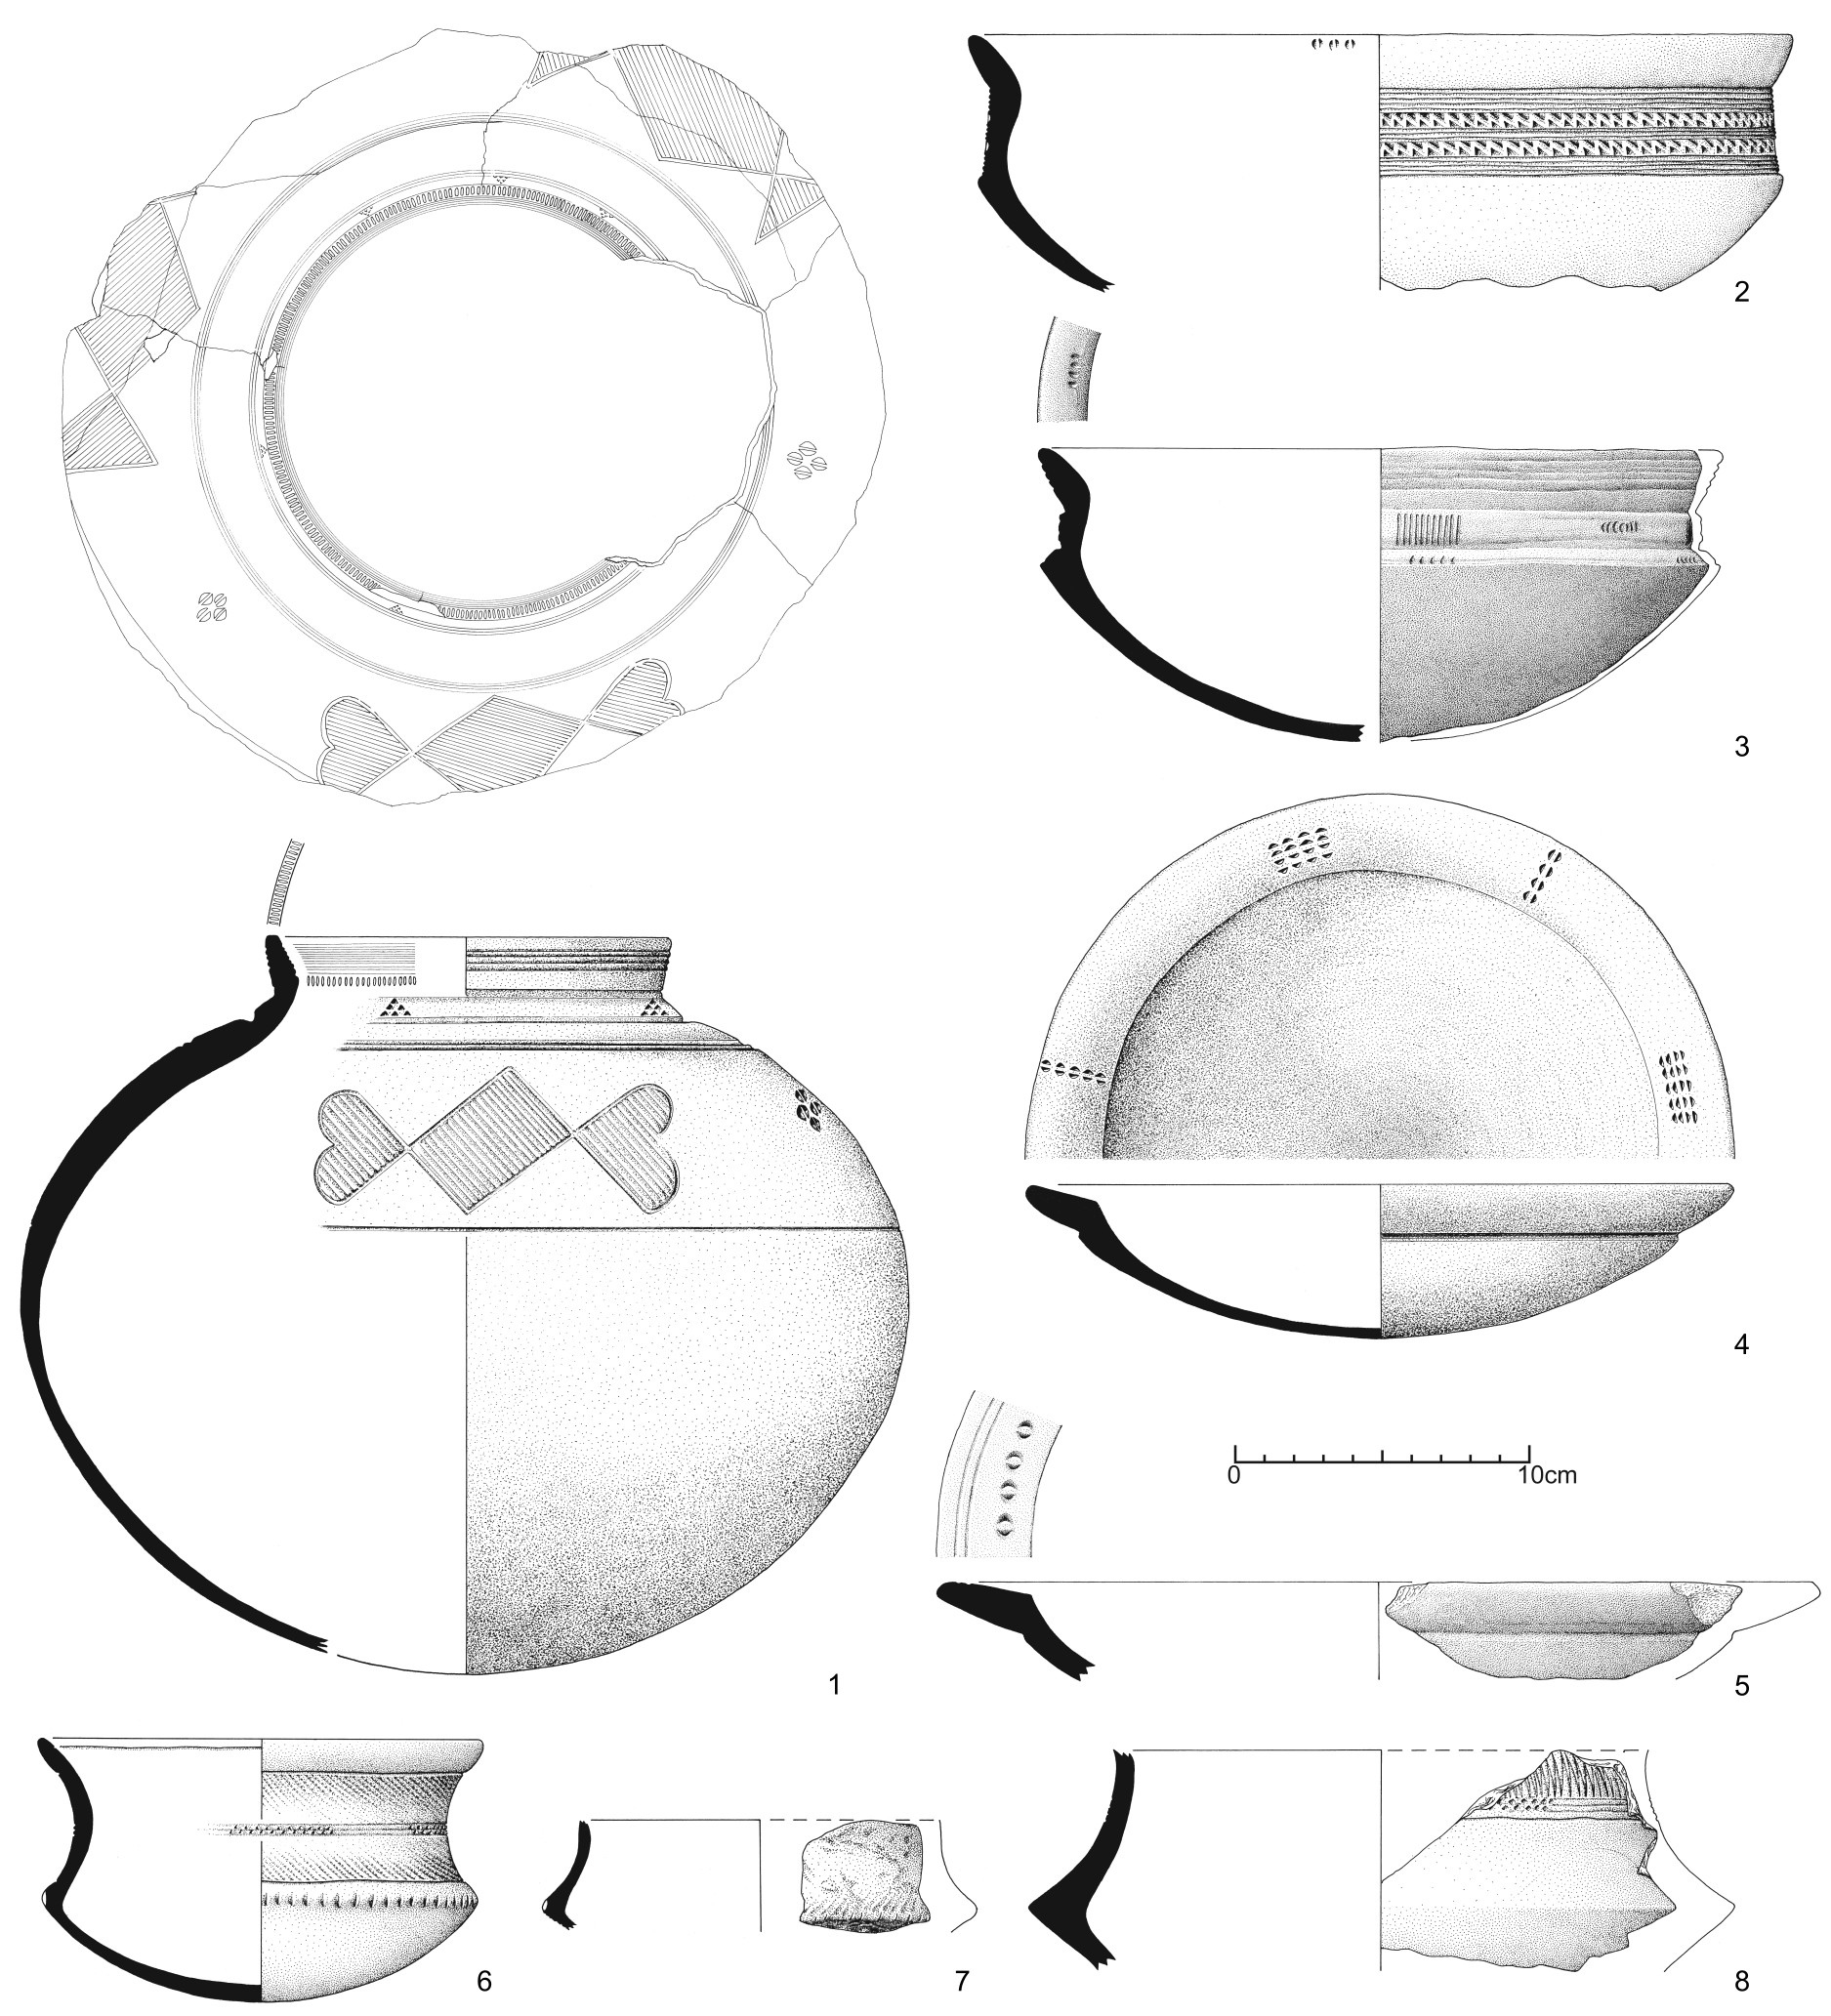
\includegraphics[width=\textwidth]{fig/NGO-Typen.pdf}
	\caption{Ngombe-Gruppe: Typvertreter aus Ngombe (Fpl.~252; Kat.-Nr.~11), Sosolo (Fpl.~241) und Bokonongo (Fpl.~250).\\1:~Taf.~43.1; 2:~Taf.~40.10; 3:~Taf.~42.15; 4:~44.1; 5:~Taf.~44.2; 6:~Taf.~42.16; 7:~Taf.~40.9; 8:~Taf.~36.13.}
	\label{fig:NGO_Typvertreter}
\end{figure*}

\begin{table*}[p]
	\centering
	{\footnotesize \begin{sftabular}{@{}lcccccc@{}}
			\toprule
			& \multicolumn{2}{c}{\textbf{Ngombe}} & \multicolumn{2}{c}{\textbf{\centering Longa}} & \multicolumn{2}{c}{\textbf{\centering Mbandaka}} \\
			& morph. & ornam. & morph. & ornam. & morph. & ornam. \\
			\midrule
			Große, bauchige Gefäße (G10a) & $\bullet$ & & & & $\circ$ & \\
			Knickwandschalen (G1a2/Typ 50) & $\bullet$ & & $\bullet$ & & & \\
			Teller (G12) & $\bullet$ & $\bullet$ & $\bullet$ & $\bullet$ & & \\ \hdashline[0.5pt/5pt]
			\textit{banfwa-nfwa}-Verzierung (V7) & \multicolumn{2}{c}{$\circ$}  & \multicolumn{2}{c}{$\bullet$} & \multicolumn{2}{c}{$\bullet$} \\
			Runde Böden (B1) & \multicolumn{2}{c}{$\bullet$} & \multicolumn{2}{c}{$\circ$} & & \\
			\bottomrule
	\end{sftabular}}
	\caption{Ngombe-Gruppe: Morphologische und ornamentale Übereinstimmungen zu den Stilgruppen Longa \parencite[121--128]{Wotzka.1995} und Mbandaka (ebd. 139--143).}
	\label{tab:NGO_Vgl_LON}
\end{table*}

\subsubsection{Ngombe-Gruppe}\label{sec:NGO-Gr}

Entlang des Unterlaufs des \mbox{Sangha} sowie dem \mbox{Likwala}-\mbox{aux}-\mbox{Herbes} und dem befahrenen Abschnitt des Kongo wurde eine Keramik erfasst, welche einerseits starke Ähnlichkeiten zu Stilgruppen des Inneren Kongobeckens, unter anderem den Gruppen Longa und Mbandaka, zeigt \parencite[121--128, 139--143]{Wotzka.1995}, andererseits aber auch deutlich eigenständige Charakteristika aufweist. Insgesamt wurden 56~GE von 15 verschiedenen Fundplätzen dieser nach der Fundstelle Ngombe am \mbox{Sangha} (Fpl. 252) benannten keramischen Stilgruppe zugerechnet. Die Hälfte aller aufgenommen Scherben der Ngombe-Gruppe sind Wandungsstücke. Zudem konnten sechs vollständige Gefäße dieser Stilgruppe zugewiesen werden. Der definierende Komplex für das Merkmalsspektrum der Ngombe-Gruppe ist die Keramikkonzentration NGO~87/102 (Kat.-Nr.~11) in Ngombe am \mbox{Sangha} (Fpl.~252; Abb.~\ref{fig:NGO_Typvertreter}).\footnote{Im Zuge der ursprünglichen Bearbeitung der Funde von 1987 fiel auf, dass aus dem Komplex NGO~87/101 aus Ngombe am \mbox{Sangha} (Fpl.~252), der das an der Oberfläche abgesammelte Material umfasst, keinerlei Funde vorliegen (\textsc{Eggert} 1990). Bei den Funden aus der an der Mündung des \mbox{Likwala}-\mbox{aux}-\mbox{Herbes} in den \mbox{Sangha} gelegenen Fundstelle Ngombe (Fpl.~283) fand sich neben dem Fundzettel für diesen Komplex noch ein weiterer Fundzettel, der mit NGO~87/101 beschriftet war. Es muss davon ausgegangen werden, dass die Funde der Komplexe NGO~87/101 aus Ngombe am \mbox{Sangha} und NGL~87/101 aus Ngombe am \mbox{Likwala}-\mbox{aux}-\mbox{Herbes} zu einem sehr frühen Zeitpunkt vermischt und beide Inventare anschließend mit der Kennung des letzten Komplexes (NGL~87/101) beschriftet wurden. Eine Vermischung der beiden Komplexe aus Ngombe selbst, des Materials von der Oberfläche (NGO~87/101) mit jenem aus der Keramikkonzentration (NGO~87/102, Kat.-Nr.~11) wurde bereits von den ersten Bearbeitern als wenig wahrscheinlich angesehen, da die Keramikkonzentration ein spezifisches Inventar weniger, aus einer Vielzahl von Fragmenten zusammensetzbarer Gefäße enthielt. Siehe Anm.~\ref{ftn:Vermischungen}.} Die daraus geborgene Keramik kann als zeitlich vergesellschaftet angesehen werden und entspricht sich in technischen wie formalen und ornamentalen Gesichtspunkten.

\paragraph{Technologische Merkmale}\hspace{-.5em}|\hspace{.5em}%
Die Scherben der Ngombe-Keramik enthalten praktisch keine nichtplastischen Partikel (89\,\%). Wenn Partikel in den Scherben beobachtbar sind, handelt es sich größtenteils um feinen Quarz. Bei 11\,\% der GE konnte ein Zusatz von zerstoßenen Keramikfragmenten im Scherben nachgewiesen werden. Ausschließlich Stücke von den beiden Fundplätzen Sosolo (Fpl.~241) und Monjolomba (Fpl.~243) am unteren \mbox{Sangha} ließen sich dem Schamott-gemagerten \textit{Fabric} 9 zuordnen (Tab.~\ref{tab:Fabrics_Bilder}). Keine Scherbe der Ngombe-Gruppe zeigt die Verwendung von rotbrennenden Tonen an. Etwa 70\,\% des Materials weist eine Färbung auf,  die eindeutig die Nutzung weißbrennender Tone anzeigt, während die Brennfarbe bei den restlichen Scherben nicht zweifelsfrei angesprochen werden konnte. Die GE der Ngombe-Gruppe zeigen durchweg geglättete Oberflächen, die in Einzelfällen auch leicht \textit{seifig} sein können. Lediglich etwa 10\,\% aller Stücke zeigen eine leicht raue Oberfläche. Die Wandungsdicke der Stücke lag im Mittel bei 6,9\,mm. 

\begin{figure*}[tb!]
	\begin{minipage}[b]{.66\textwidth}
		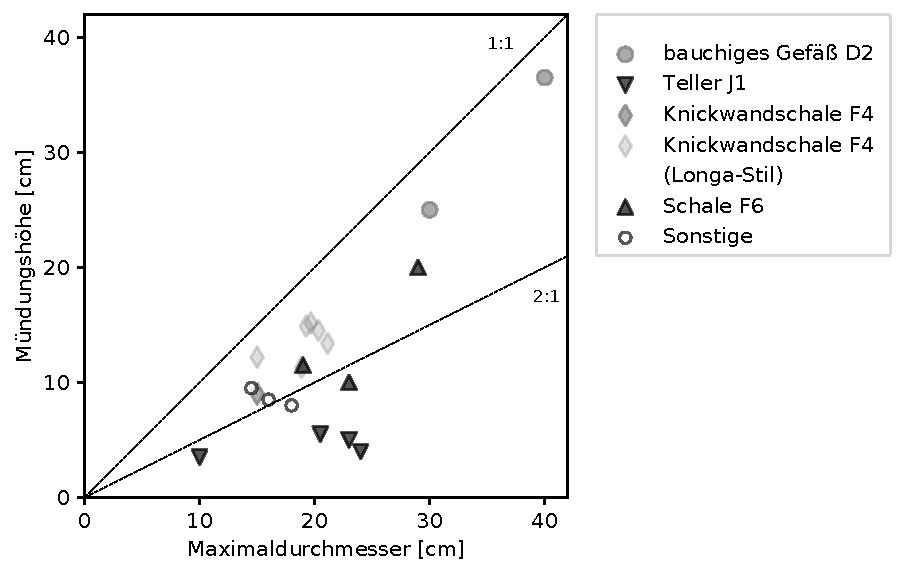
\includegraphics[width=\textwidth]{fig/NGO_Proportionen.pdf}
	\end{minipage}\hfill
	\begin{minipage}[b]{.33\textwidth}
		\caption{Ngombe-Gruppe: Proportionen (Knickwandschalen der Longa-Gruppe nach \textsc{Wotzka} 1995: 455 Taf.~21.2, 485 Taf.~51.9--10, 501 Taf.~67, 521 Taf.~87.4, 526 Taf.~92.6).\label{fig:NGO_Proportionen}}
	\end{minipage}
\end{figure*}

\paragraph{Formen}\hspace{-.5em}|\hspace{.5em}%
Bei 40 der insgesamt 56~GE der Ngombe-Gruppe konnte die Gefäßform bestimmt werden, allerdings war aufgrund von starker Fragmentierung bei 25\,\% eine sichere Ansprache nicht möglich. Den größten Anteil innerhalb der Keramik der Ngombe-Gruppe machen große Gefäße mit kurzem Kragen- oder nur leicht ausbiegendem Rand vom Typ D2 (40\,\%; Abb.~\ref{fig:NGO_Typvertreter}; Taf.~70.1) sowie Teller mit einem deutlichen Profilknick an der Innenseite aus (J1; 25\,\%; Abb.~\ref{fig:NGO_Typvertreter}.4--5).\footnote{Die Teller der Ngombe-Gruppe entsprechen morphologisch wie ornamental dem Typ~50 der Longa-Gruppe aus dem Inneren Kongobecken (\textsc{Wotzka} 1995: 121; Tab.~\ref{tab:NGO_Vgl_LON}).} Die großen, stark bauchigen Töpfe der Ngombe-Gruppe vom Typ D2 haben Durchmesser von bis zu 40\,cm, bei einer Höhe zwischen 25--36,5\,cm (Abb.~\ref{fig:NGO_Proportionen}). Die Teller des Typs J1 erreichen Durchmesser von bis zu 24\,cm und sind dabei zwischen 3,5--7\,cm hoch. Daneben umfasst das Formenspektrum auch kleine, flache Schalen mit Bauchabsatz und ausbiegendem Rand (Typ~E6; 10\,\%; Taf.~36.16--17, 38.15, 57.15) und flache Schalen mit scharfem Absatz im Bauchbereich und kurzem, ausbiegendem Rand (Typ~F6; 8\,\%; Abb.~\ref{fig:NGO_Typvertreter}.2--3). Etwas seltener finden sich flache Schalen mit starkem Bauchknick und deutlich ausgeprägtem, konkavem Halsbereich (Typ~F4; Abb.~\ref{fig:NGO_Typvertreter}.6--8)\footnote{Diese Form entspricht morphologisch den Knickwandschalen der Longa-Gruppe des Inneren Kongobeckens (Typ~44; \textsc{Wotzka} 1995: 121; 485~Taf.~14,9--10). Die Stücke der Ngombe-Gruppe des nordwestlichen Kongobeckens weisen jedoch eine andere Ornamentik als die Longa-Keramik auf.}, leicht bauchige Töpfe (Typ~C2) sowie Töpfe ohne ausgeprägten Halsbereich (Typ~E1). Das Gros der Ränder zeigt runde (M1; 42\,\%) sowie spitz (M2; 35\,\%) abgeschlossene Randlippen. In geringerem Maße fanden sich auch nach außen schräg abgestrichene Mündungsabschlüsse (M5, 12\,\%). Die am häufigsten angetroffene Randform innerhalb der Ngombe-Gruppe sind flach ausbiegende Ränder mit deutlichem Profilknick (B1.5; 32\,\%)\footnote{Die als B1.5 katalogisierte Randform entspricht den Typen R62 beziehungsweise R69 aus dem Inneren Kongobecken (\textsc{Wotzka} 1995: 122, 436 Taf.~2).}, welche den oben genannten Tellern des Typs J1 zuzuordnen sind. Die für die Ngombe-Gruppe charakteristischen großen, stark bauchigen Gefäße vom Typ D2 zeigen eine gewisse Heterogenität der Randgestaltung: durchweg kurze Varianten der Randformen A1, B1 sowie B2. Die zweithäufigste Randform innerhalb der Ngombe-Gruppe ist ein kurzer, leicht ausbiegender Rand (B1) an Schalen des Typs E6 und F6, die einen leicht konvexen Halsbereich sowie Absatz im Bauchbereich aufweisen. Bei 13~GE der Ngombe-Gruppe konnte die Form des Gefäßbodens bestimmt werden; in allen Fällen war der Boden rund ausgeformt (Typ~B1).

\paragraph{Verzierungen}\hspace{-.5em}|\hspace{.5em}%
Die Keramik der Ngombe-Gruppe ist grundsätzlich nur sporadisch verziert. Das mit Abstand am häufigsten angetroffene Verzierungselement sind horizontale Rillen (Tab.~\ref{tab:Verzierungselemente}: 02.1; 41\,\%). Diese finden sich durchweg auf der Innenseite und außen an den Rändern sowie im Hals- und Schulterbereich der Gefäße (Anlage~4\subref{fig:NGO_Verz}). Deutlich seltener und vor allem innen wie außen im Rand-, Schulter- und Bauchbereich finden sich horizontale Reihen aus einfachen Eindrücken (Tab.~\ref{tab:Verzierungselemente}: 04.15; 10\,\%). Eine Eigenheit der Ngombe-Keramik sind Gruppen aus kleinen, halbrunden Eindrücken beziehungsweise Einkerbungen, die fast ausschließlich an der Innenseite der Ränder zu finden sind (Tab.~\ref{tab:Verzierungselemente}: 04.5; 8\,\%). Des Weiteren umfasst das Spektrum an Verzierungselementen der Ngombe-Gruppe eine breite Palette von Ritz- oder Eindruckelementen (Tab.~\ref{tab:Verzierungselemente}: 01.1--3, 01.6, 01.8, 02.2--3, 02.5, 04.2--4, 04.8--9, 04.11--12, 04.17--18) sowie \textit{banfwa-nfwa}-Verzierungen (Tab.~\ref{tab:Verzierungselemente}: 08; 4\,\%) auf der Innenseite der Ränder sowie im Hals- und Schulterbereich (Anlage~4\subref{fig:NGO_Verz}). Die Ngombe-Gefäße zeigen eine klare Fokussierung der Verzierungen auf die Innenseite der Ränder sowie den Schulter- und Halsbereich. Insgesamt 75\,\% aller Verzierungen finden sich in diesen Abschnitten der Gefäße. Auf den Gefäßbäuchen finden sich nur sehr vereinzelt Verzierungen und die Gefäßunterteile sind bis auf Einzelfälle unverziert (\mbox{Anlage}~4\subref{fig:NGO_Verz}). Nur eine GE zeigt \textit{banfwa-nfwa} (Tab.~\ref{tab:Verzierungselemente}: 08) am Bodenansatz (Taf.~40.7).

\begin{figure*}[p]
	\centering
	\includegraphics[width=\textwidth]{fig/NGO_Verbreitung.pdf}
	\caption{Ngombe-Gruppe: Verbreitung.}
	\label{fig:NGO_Verbreitung}
\end{figure*}

\paragraph{Datierung}\hspace{-.5em}|\hspace{.5em}%
Für die Keramik der Ngombe-Gruppe liegen keine absoluten Daten vor. Der einzig potenziell datierbare Komplex, der für die Beschreibung der Gruppe bestimmenden Keramikkonzentration NGO~87/102 (Kat.-Nr.~11) in Ngombe am mittleren \mbox{Sangha} (Fpl.~252), konnte in den 1980er Jahren leider nicht direkt datiert werden.\footnote{Eine für eine Radiokohlenstoffdatierung vorgesehene Probe wurde nach Kiel eingeschickt, erbrachte aber nach der Aufbereitung keine ausreichenden Anteile organischen Materials. Nachforschungen ergaben leider kein weiteres datierbares Material aus diesem Komplex.} Mit Ausnahme dieses Komplexes stammt alles der Ngombe-Gruppe zugeordnete Fundmaterial von Oberflächenabsammlungen. Die Datierung der Ngombe-Keramik kann folglich lediglich anhand relativchronologischer Bezüge abgeleitet werden. Die der Ngombe-Gruppe zugeordnete Keramik weist deutliche Übereinstimmungen mit der Keramik der Longa-Gruppe des Inneren Kongobeckens sowie leichte Ähnlichkeiten zur Mbandaka-Gruppe auf (Tab.~\ref{tab:NGO_Vgl_LON}; \textsc{Wotzka} 1995: 121--128). Gerade die stark rundbauchigen Grundformen und abgesetzten Schulterpartien sowie die Fokussierung der Verzierung auf die Rand- und Schulterzonen erinnern an die Mbandaka-Gruppe des Inneren Kongobeckens (ebd. 139--143). Die Ngombe-Gruppe zeichnet sich, wie auch die Longa-Keramik (ebd. 123), durch runde Böden aus. Knickwandschalen des Typs F4 finden sich in beiden Stilgruppen. Jedoch weisen die GE der Longa-Gruppe (ebd. 455 Taf.~21.1--5, 456 Taf.~22.1--8, 475 Taf.~41.9, 485 Taf.~51.9--10, 503 Taf.~69.6--9, 507 Taf.~73.1--29) eine sehr viel elaboriertere Verzierung auf.

Die absolute Datierung der Longa-Gruppe ist gegenwärtig als unklar zu bezeichnen. Einerseits weist die Stilgruppe einen verbindenden Charakter zwischen den früheren Stilgruppen, vor allem Bokuma und Bokele, auf, andererseits stellt \textsc{Wotzka} (ebd. 127) fest, dass sie sich problemlos an das jüngere Ende der von ihm entwickelten Keramiksequenz anbinden lässt, welches vornehmlich durch die Bondongo-Gruppe charakterisiert ist. Die drei für die Longa-Gruppe vorliegenden Radiokohlenstoffdatierungen streuen vom 1.~Jt. v.~Chr. bis in das 12./13.~Jh. n.~Chr. (ebd. 127 Tab.~53).\footnote{Eine neuere Evaluation Wotzkas ergab eine höhere Wahrscheinlichkeit dafür, dass die jüngste der drei Datierungen, die in das 12./13.~Jh. n.~Chr. fällt (\textsc{Wotzka} 1995: 127 Tab.~53: Hv-11572), am ehesten repräsentativ für die chronologische Stellung der Stilgruppe ist. Siehe Kap.~\ref{sec:ICB_StilGrDatierungen}) und Anm.~\ref{ftn:fstafrikaWebStilGr-Tafeln}.}

Die Keramik der Mbandaka-Gruppe wird von Wotzka (ebd. 143) in eine zeitliche Nähe zur ins 11.--14.~Jh. n.~Chr. datierenden Bondongo-Keramik (ebd. 138 Tab.~58) gestellt, die wiederum starke Ähnlichkeiten zur Longa-Keramik aufweist. Für die Anbindung der Ngombe-Gruppe kann, bis eine direkte Datierung eines entsprechende Funde aufweisenden Komplexes vorliegt, nur eine den Stilen Longa und Mbandaka entsprechende, vom 12.--14.~Jh. n.~Chr. reichende Zeitstellung angenommen werden.

\paragraph{Verbreitung}\hspace{-.5em}|\hspace{.5em}%
Die Keramik der Ngombe-Gruppe wurde an insgesamt 15 verschiedenen Fundstellen im Bereich der Flussläufe des Kongo, \mbox{Sangha} sowie \mbox{Likwala}-\mbox{aux}-\mbox{Herbes} angetroffen. Das Verbreitungsgebiet besteht dabei aus zwei Kerngebieten; zum einen am mittleren \mbox{Sangha} zwischen Inyenge (Fpl.~249) und Ngombe (Fpl.~252) und zum anderen unmittelbar im Mündungsgebiet des \mbox{Sangha} in den Kongo (Abb.~\ref{fig:NGO_Verbreitung}). Die meisten Funde stammen aus dem letzteren Gebiet und hier vor allem von den beiden Plätzen Sosolo (Fpl.~241) und Monjolomba (Fpl.~243). Im Bereich nördlich, beziehungsweise flussauf von Ngombe (Fpl.~252), sowie am Kongo und \mbox{Likwala}-\mbox{aux}-\mbox{Herbes} fand sich ausschließlich Material, dessen Zuweisung zur Ngombe-Gruppe unter Vorbehalt erfolgte (Abb.~\ref{fig:NGO_Verbreitung}). Im Mündungsgebiet des Likwala-aux-Herbes, in Boleko (Fpl.~285), fanden sich lediglich zwei sicher der Ngombe-Gruppe zuweisbare GE.

\begin{figure*}[tb]
	\begin{minipage}[b]{.8\textwidth}
		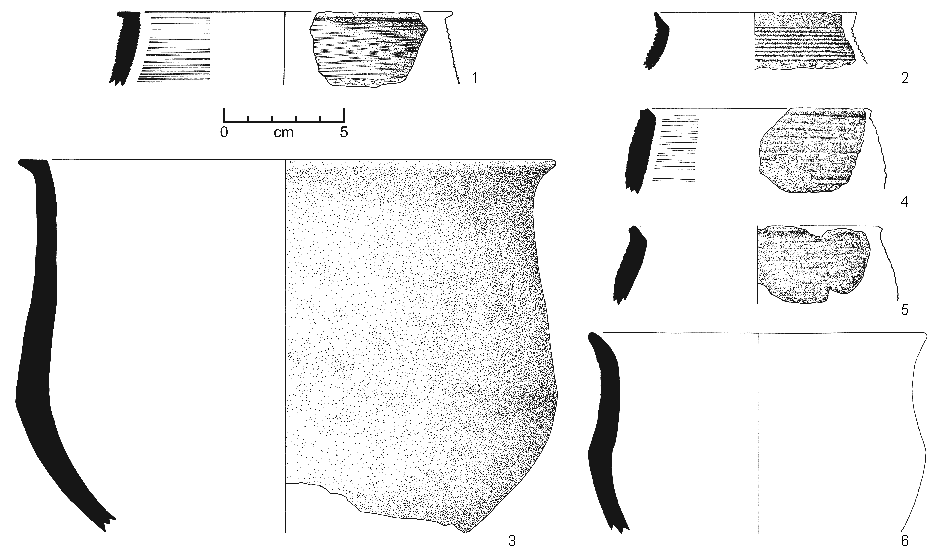
\includegraphics[width=.95\textwidth]{fig/MAT-Typen.pdf}
	\end{minipage}\hfill
	\begin{minipage}[b]{.2\textwidth}
		\caption{Matoto-Gruppe: Typvertreter.\\1:~Taf.~59.26; 2:~Taf.~59.1; 3:~Taf.~87.3; 4:~Taf.~59.30; 5:~Taf.~59.29; 6:~Taf.~21.2.}
		\label{fig:MAT_Typvertreter}
	\end{minipage}
\end{figure*}

\subsubsection{Matoto-Gruppe}\label{sec:MAT-Gr}

Die Matoto-Gruppe beschreibt eine nahezu im gesamten Arbeitsgebiet angetroffene Keramik, welche sich vor allem durch ihre charakteristischen Gefäßmorphologie auszeichnet. Dabei handelt es sich konkret um Gefäße mit gerader Wandung und sehr kurzen, teilweise scharf umbiegenden Rändern (Abb.~\ref{fig:MAT_Typvertreter}). Insgesamt konnten 60 GE dieser Stilgruppe zugeordnet werden, während 15 weitere GE nur unter Vorbehalt der Matoto-Gruppe zuzurechnen sind. Überdies wurden weitere 33 Randscherben aus Mandombe (Fpl.~259) und Motoli (Fpl.~261) am \mbox{Sangha}, die sämtlich sicher der Matoto-Gruppe zuordnet werden konnten, summarisch erfasst. Die Matoto-Gruppe setzt sich fast ausschließlich aus Randstücken zusammen (95\,\%). Lediglich ein hinreichend vollständiges Gefäß (Abb.~\ref{fig:MAT_Typvertreter}.3) konnte dieser Stilgruppe zugewiesen werden. Während ein großer Teil des keramischen Materials der Matoto-Gruppe aus Mandombe am mittleren \mbox{Sangha} (Fpl.~259) stammt, insgesamt wurden hier 31~GE und 30 ausgezählte Randstücke der Matoto-Gruppe nachgewiesen, wurden an insgesamt 17 weiteren Fundorten entlang der Flussläufe des \mbox{Sangha}, \mbox{Likwala}-\mbox{aux}-\mbox{Herbes} und \mbox{Ubangi} sowie am Lua immer wieder vereinzelte GE der Matoto-Gruppe (\textless\,9~GE) bei Surveys entdeckt. Mit Blick auf die individuell aufgenommenen GE macht das Inventar aus Mandombe 41\,\% aller der Matoto-Gruppe zugerechneten Stücke aus.\footnote{Da die Fundstelle Mandombe (Fpl.~259) bereits als eponymer Name für eine andere keramische Stilgruppe herangezogen wurde (Kap.~\ref{sec:MDB-Gr}), wurde die mit neun GE zwar eindeutig ärmere, jedoch auch das zweitgrößte Fundinventar aufweisende Fundstelle Matoto am mittleren \mbox{Sangha} (Fpl.~264) als eponyme Fundstelle für die Stilgruppe ausgewählt. Matoto liegt nur etwa 20\,km stromauf beziehungsweise nördlich von Ma"-ndo"-mbe und fällt in das Hauptverbreitungsgebiet der Stilgruppe.} Etwa 87\,\% aller Stücke stammen aus Absammlungen von Oberflächen. Die Funde aus Mandombe wurden vornehmlich zwischen aufgelassenen, alten Hausstellen gemacht. Acht GE der Matoto-Gruppe wurden oberhalb der Grube MLB~85/1-3-1 (Kat.-Nr.~1) in Maluba am Lua (Fpl.~230) erfasst.\footnote{Im ersten Abtrag fanden sich sechs GE und in den Abträgen 3 sowie 4 jeweils ein weiteres Randstück, das der Matoto-Gruppe zugerechnet werden kann.} Zwei weitere GE der Matoto-Gruppe wurden im zweiten und dritten Abtrag der Grabung PIK~87/1 gefunden (Kat.-Nr.~8; Taf.~48.11).


\paragraph{Technologische Merkmale}\hspace{-.5em}|\hspace{.5em}%
Die Scherben der Matoto-Gruppe zeigen eine starke Heterogenität der \textit{Fabrics}. Fast dreiviertel aller Scherben weisen hohe (54\,\%) bis sehr hohe (20\,\%) Anteile nichtplastischer Partikel auf. Diese sind größtenteils den Größenklassen \textit{medium} (32\,\%) sowie \textit{coarse} (46\,\%) zuzurechnen. Es handelt sich fast ausschließlich um Quarzsande (84\,\%). Selten enthalten die Scherben auch ausgebrannte Organik sowie Glimmer oder Laterit. In Bezug auf die Färbung der Scherben weisen über die Hälfte aller Stücke (51\,\%) auf die Nutzung weißbrennender Tone hin, während jeweils etwa ein Viertel der Stücke rotbrennende Tone andeuten (25\,\%) oder keine Aussagen zulassen (24\,\%). Nur 26\,\% der Scherben zeigen geglättete Oberflächen, während 53\,\% leicht raue und 18\,\% deutlich raue Oberflächen aufweisen. Die GE der Matoto-Gruppe zeigen eine mittlere Wandungsdicke von 6,2\,mm.

\begin{figure*}[p]
	\centering
	\includegraphics[width=\textwidth]{fig/MAT_Verbreitung.pdf}
	\caption{Matoto-Gruppe: Verbreitung.}
	\label{fig:MAT_Verbreitung}
\end{figure*}

\paragraph{Formen}\hspace{-.5em}|\hspace{.5em}%
Lediglich bei zwei GE der Matoto-Gruppe konnte die Gefäßform sicher angesprochen werden, während bei acht weiteren GE eine Ansprache der Gefäßform unter Vorbehalt vorgenommen werden konnte. Die beiden sicher angesprochenen Stücke zeigen ein gerades beziehungsweise nur leicht konkaves Oberteil, einen leichten Bauchknick sowie ein konvexes Unterteil und sind der Gefäßform F1 zuzurechnen. Sie stammen vom Likwala-aux-Herbes, Flusskilometer~401 (Fpl.~301; Abb.~\ref{fig:MAT_Typvertreter}.3) sowie aus Mboko~I am \mbox{Ubangi} (Fpl.~217; Abb.~\ref{fig:MAT_Typvertreter}.6). Obschon viele der Randstücke zu einer sehr ähnlichen Gefäßform gehört haben könnten (Abb.~\ref{fig:MAT_Typvertreter}.1--2, 4--5), lässt sich aufgrund mangelnder Erhaltung der Gefäßprofile keine belastbare Aussage treffen. Der maximale Durchmesser der Gefäße schwankt zwischen 14--22\,cm, bei einer Mündungshöhe von 11,5--17\,cm.  Da nur wenige größere Scherben der Matoto-Gruppe vorhanden sind, liegen auch kaum Informationen über die Ausgestaltung der Gefäßbäuche vor. Lediglich bei fünf GE war der Gefäßbauch erhalten. Vier GE zeigen die typischen, leichten Bauchknicke, die für die Gefäßform F1 charakteristisch sind. Die bestimmenden Randformen der Matoto-Keramik sind kurz umgelegte (A2; 39\,\%; Abb.~\ref{fig:MAT_Typvertreter}.1, 3) sowie ausbiegende Ränder (B1; 44\,\%; Abb.~\ref{fig:MAT_Typvertreter}.2, 4--5). Die Mündungsabschlüsse der Ränder sind regelhaft spitz zulaufend (M2; 34\,\%) oder gerillt (M4; 33\,\%). Deutlich seltener fanden sich rund abgeschlossene (M1; 9\,\%) sowie schräg nach außen abgestrichene Mündungen (M5; 7\,\%). Der Halsbereich der Matoto-Gefäße ist häufig leicht kegelförmig bis zylindrisch. Nur sechs GE zeigen einen ausgeprägten Schulterbereich, welcher entweder gerade oder leicht konvex ist. Bei zwei GE, beide stammen aus Yumba am \mbox{Likwala}-\mbox{aux}-\mbox{Herbes} (Fpl.~289), ließ sich die Form des Gefäßbodens ermitteln. Beide Stücke weisen runde Böden auf (B1). Die Zuordnung beider Stücke zur Matoto-Gruppe ist jedoch nicht zweifelsfrei. Aus dem restlichen Fundmaterial sind keine Bodenscherben der Matoto-Gruppe bekannt, so dass keine belastbaren Aussagen über die Gestaltung der Böden der Matoto-Keramik gemacht werden können.

\paragraph{Verzierungen}\hspace{-.5em}|\hspace{.5em}%
Die Verzierungen der Matoto-Gruppe werden von horizontalen Rillen (Tab.~\ref{tab:Verzierungselemente}: 02.1) bestimmt, die 84\,\% aller Verzierungselemente ausmachen und sich fast ausschließlich und zu gleichen Teilen auf der Innenseite der Ränder sowie im Halsbereich finden (Abb.~\ref{fig:MAT_Typvertreter}.1--2,4; Anlage~4\subref{fig:MAT_Verz}). Insgesamt lassen sich 87\,\% aller beobachteten Verzierungselemente diesen beiden Gefäßzonen zuordnen. Unterhalb des Schulterbereichs ließen sich keine Verzierungen beobachten, was allerdings auch der Tatsache geschuldet ist, dass sich die Matoto-Gruppe fast ausschließlich aus Randscherben zusammensetzt und andere Gefäßzonen deutlich unterrepräsentiert sind. Neben den horizontalen Rillen finden sich nur sehr selten weitere Verzierungselemente. Unter anderem handelt es sich dabei um Reihen aus kleinen diagonalen oder vertikalen Ritzlinien (Tab.~\ref{tab:Verzierungselemente}: 04.15; 7\,\%), Reihen aus dreieckigen oder quadratischen Eindrücken (Tab.~\ref{tab:Verzierungselemente}: 04.12; 3\,\%) sowie runden Eindrücken (Tab.~\ref{tab:Verzierungselemente}: 04.11; 2\,\%) und diagonales Schachbrettmuster (Tab.~\ref{tab:Verzierungselemente}: 01.2; 1\,\%; Abb.~\ref{fig:MAT_Typvertreter}.4--5). Alle beobachteten Verzierungen sind grundsätzlich sehr fein ausgeführt.

\paragraph{Datierung}\hspace{-.5em}|\hspace{.5em}%
Für die Keramik der Matoto-Gruppe liegen keine direkten Datierungen vor. Lediglich im Fundgut, das der Bestattung in MLB~85/1-4-3 (Kat.-Nr.~3) in Maluba am Lua zugewiesen wurde, fanden sich neben Batalimo-Maluba-Keramik auch Stücke, die der Matoto-Gruppe zugerechnet werden können. Zwei Radiokohlenstoffdatierungen an Knochenmaterial datieren in das 11.--14.~Jh. n.~Chr. (Tab.~\ref{tab:MLB85_1-4-3_14C}). Da das mit der Bestattung assoziierte keramische Material jedoch nicht als dezidierte \textit{Beigabe} zu interpretieren ist (siehe Kat.-Nr.~3), kann dieser Datierungsansatz lediglich als \textit{terminus ante quem} herangezogen werden; die Matoto-Gruppe muss also im 11.--14.~Jh. n.~Chr. bereits bestanden haben.

Stilistische Vergleiche zu anderen Stilgruppen des Arbeitsgebietes ergeben sich nur zu den Gruppen Dongo (Kap.~\ref{sec:DON-Gr}) sowie Konda (Kap.~\ref{sec:KON-Gr}). Beide weisen, wie die Matoto-Keramik, im Randbereich eine Verzierung aus feinen Rillen auf. Die Keramik der Dongo-Gruppe weist, ähnlich der Matoto-Keramik, auch eher kurze, gerade ausbiegende Ränder sowie Grundformen mit teilweise eher schwach geschweiften Wandungen auf. Keine der als Vergleich heranzuziehenden Stilgruppen ist jedoch sicher im Chronologieschema (Abb.~\ref{fig:Chronologiesystem}) zu verankern, wodurch auch die genannten Bezüge zur Matoto-Gruppe starken Vorbehalten unterliegen.

Vor dem gegenwärtigen Quellenstand kann keine sichere chronologische Ansprache der Matoto-Keramik erfolgen. Einzig die Beobachtung entsprechender Stücke in der Verfüllung des Grabes MLB~85/1-4-3 in Maluba (Kat.-Nr.~3) zeigt an, dass die Stilgruppe zu diesem Zeitpunkt bereits bestanden haben muss. Vorläufig wird sie daher an den Beginn der Jüngeren Eisenzeit im Arbeitsgebiet beziehungsweise in das 11.--14.~Jh. n.~Chr. datiert.

\paragraph{Verbreitung}\hspace{-.5em}|\hspace{.5em}%
Die Keramik der Matoto-Gruppe ist nahezu über das gesamte Arbeitsgebiet verbreitet (Abb.~\ref{fig:MAT_Verbreitung}). Den nördlichsten Verbreitungspunkt bildet dabei Mboko~I am oberen \mbox{Ubangi} (Fpl.~217). Das Kerngebiet ist jedoch eine kleine Region am mittleren \mbox{Sangha} nördlich von Pikunda, zwischen Molanda (Fpl.~258) und der namensgebenden Fundstelle Matoto (Fpl.~264). Aus diesem Bereich stammen 88\,\% aller sicher der Matoto-Gruppe zugewiesenen GE. Am \mbox{Likwala}-\mbox{aux}-\mbox{Herbes} fand sich bei Flusskilometer 401 (Fpl.~301) im Uferbereich eines stark mit Termiten-Hügeln durchzogenen Gebietes ein unverziertes Gefäß des Matoto-Stils (Abb.~\ref{fig:MAT_Typvertreter}.3).

\begin{figure*}[p]
	\centering
	\includegraphics[height = .9\textheight]{fig/EBA-Typen.pdf}
	\caption{Ebambe-Gruppe: Typvertreter.\\1:~Taf.~55.4; 2:~Taf.~54.15; 3:~Taf.~41.9; 4:~Taf.~89.4; 5:~Taf.~49.16; 6:~Taf.~55.8; 7:~Taf.~56.15; 8:~Taf.~82.9; 9:~Taf.~62.14; 10:~Taf.~82.4; 11:~Taf.~90.1.}
	\label{fig:EBA_Typvertreter}
\end{figure*}

\begin{figure*}[tb]
	\begin{minipage}[b]{\columnwidth}
		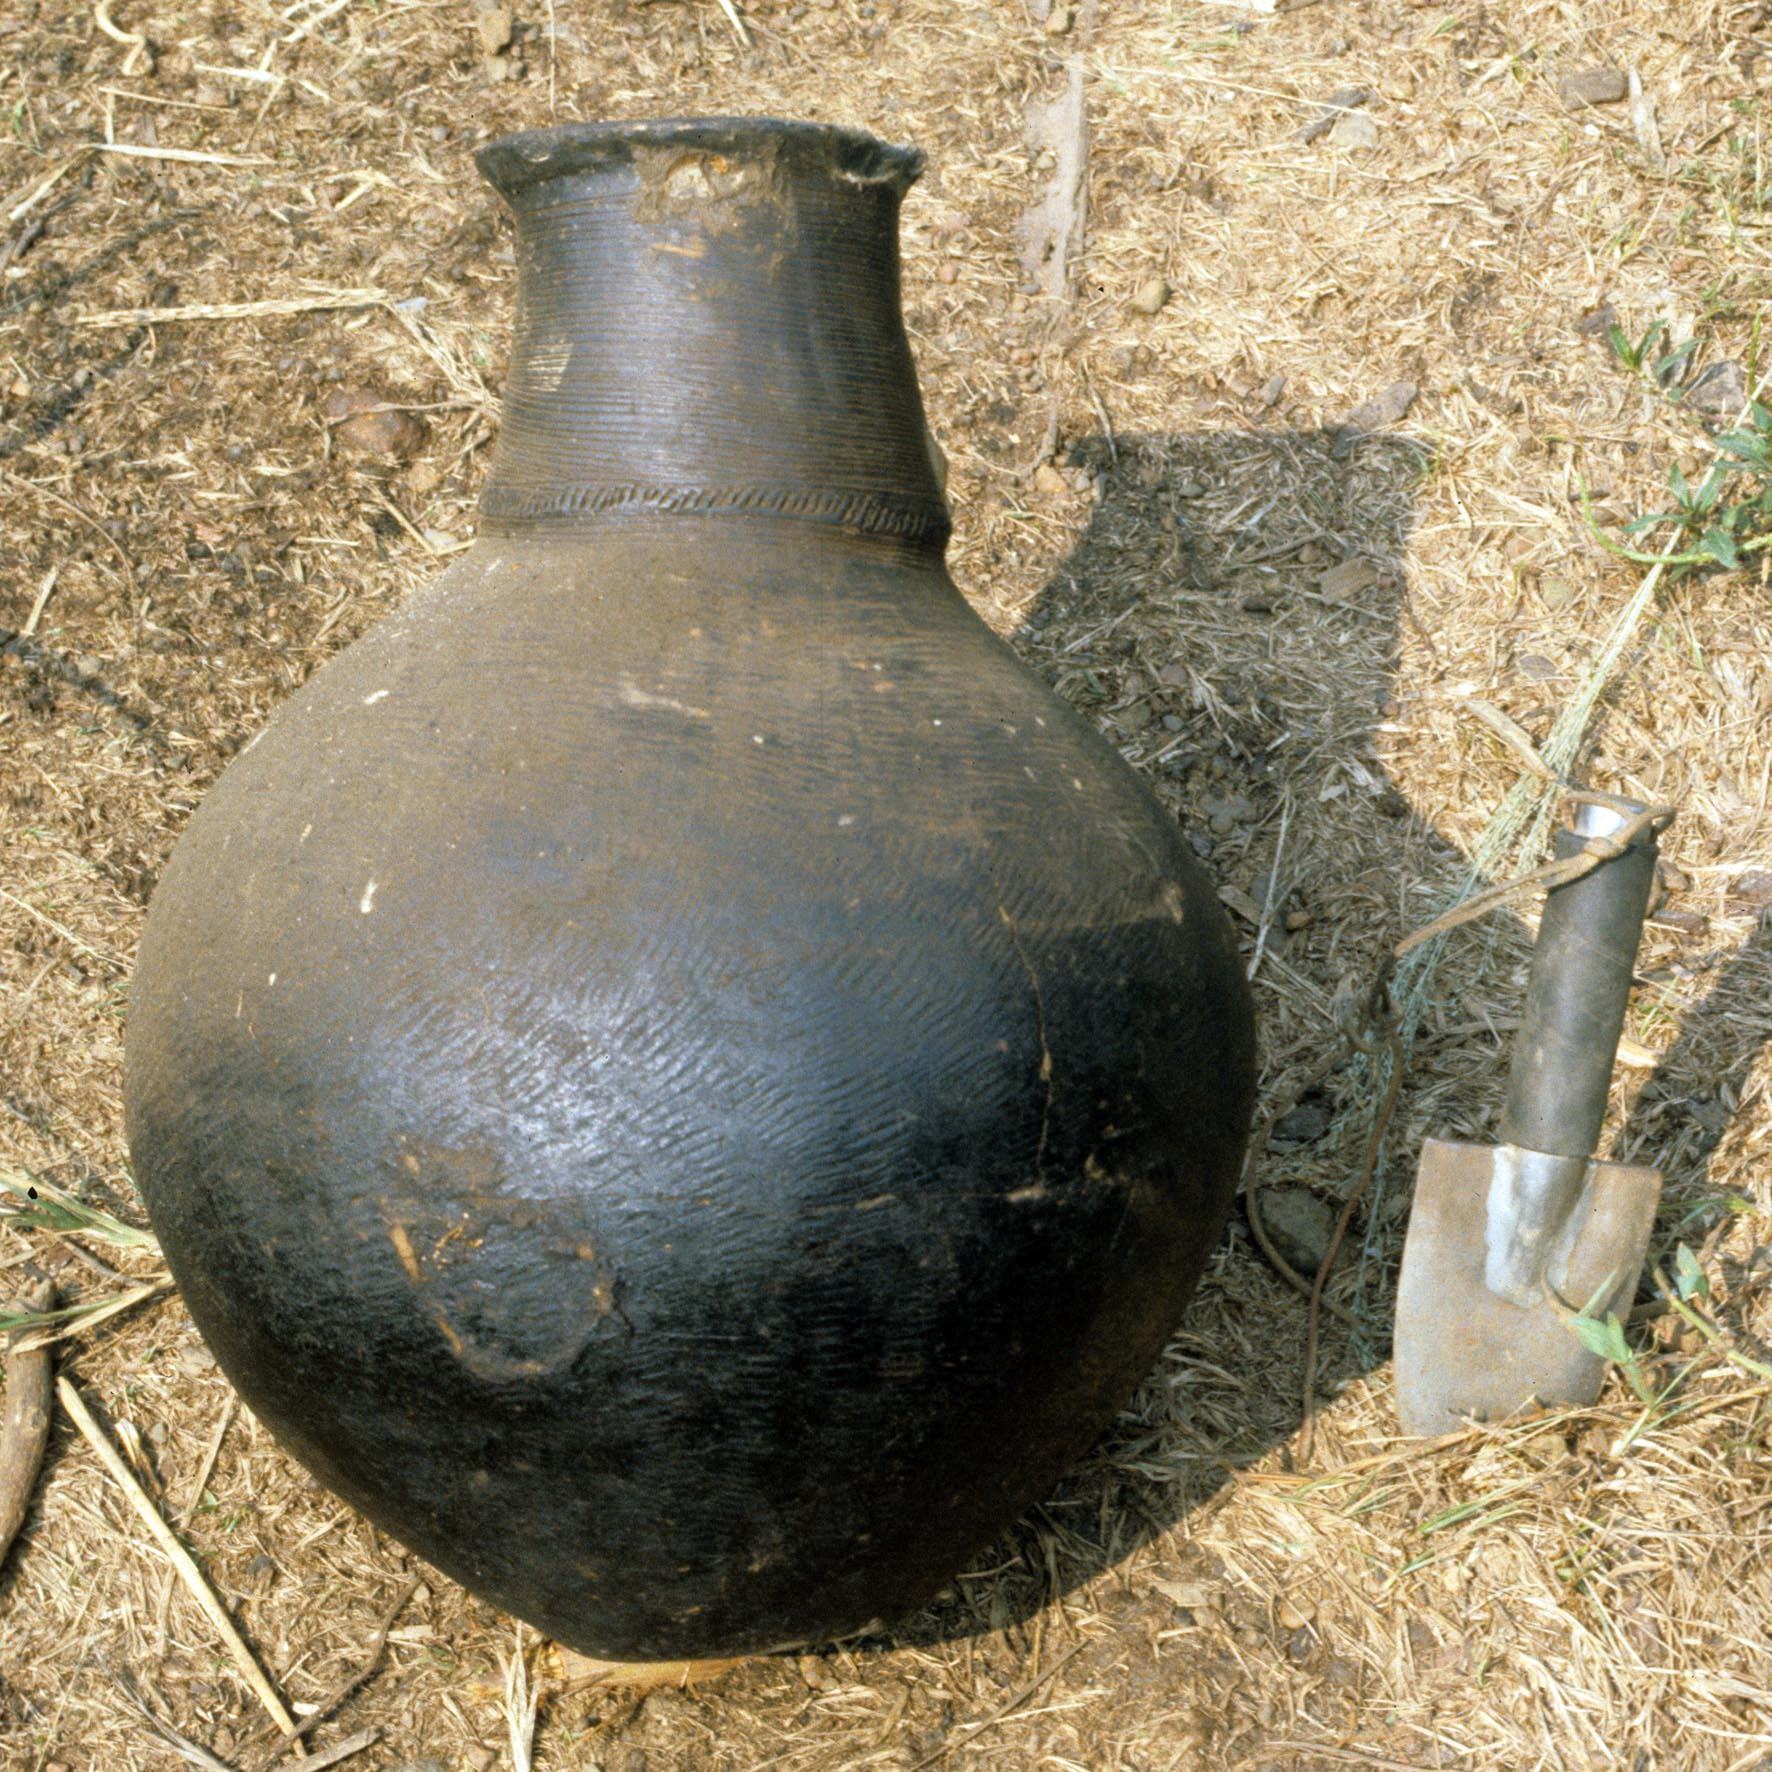
\includegraphics[width=\textwidth]{fig/BYN87-101_Gef_aus_Epena_E87-023-10.jpg}
	\end{minipage}\hfill
	\begin{minipage}[b]{\columnwidth}
		\caption{Ebambe-Gruppe: Flasche vom Typ A2 der Ebambe-Gruppe in Boyenge am Unterlauf des \mbox{Likwala}-\mbox{aux}-\mbox{Herbes} (Fpl.~284). Der Gefäßkörper ist mit flächigem \textit{banfwa-nfwa} (Tab.~\ref{tab:Verzierungselemente}: 08) verziert, während der Hals horizontale, feine Rillen (Tab.~\ref{tab:Verzierungselemente}: 02.1) sowie diagonal gestellte Eindrücke (Tab.~\ref{tab:Verzierungselemente}: 04.12) aufweist. Nach Angabe der lokalen Bevölkerung stammt das Gefäß aus Epena (Fpl.~306), wo entsprechende Formen seinerzeit noch getöpfert worden sein sollen (Foto: M. K. H. Eggert, 1987).}\label{fig:EBA_BoyengeE8702310}
	\end{minipage}
\end{figure*}

\subsubsection{Ebambe-Gruppe}\label{sec:EBA-Gr}

Die Ebambe-Gruppe, benannt nach einer Fundstelle am mittleren \mbox{Likwala}-\mbox{aux}-\mbox{Herbes} (Fpl.~297), beschreibt eine vor allem entlang des \mbox{Sangha} und \mbox{Likwala}-\mbox{aux}-\mbox{Herbes} verbreitete Keramik, die enge Beziehungen zur rezenten Epena-Keramik (Kap.~\ref{sec:EPE-Gr}) sowie Ähnlichkeiten zu Stilgruppen des Inneren Kongobeckens aufweist (Tab.~\ref{tab:EBA_VglICB}). Die chronologische Stellung des Stils lässt sich nicht genauer als auf das 2.~Jt. n.~Chr. eingrenzen (siehe unten). Insgesamt umfasst die Ebambe-Gruppe 280~GE. Weitere 520 Einzelscherben ließen sich nur unter Vorbehalt und aufgrund einzelner Merkmale zuweisen: dazu zählen vor allem Stücke mit der nur bei dieser Stilgruppe in diesem Maße beobachteten, flächigen \textit{banfwa-nfwa}-Verzierung. Aufgrund der starken Fragmentierung der Stücke und da es sich größtenteils um ansonsten wenig diagnostische Wandungsfragmente handelte, wurden sie lediglich ausgezählt.\footnote{91\,\% der 520 ausgezählten Stücke sind Fragmente der Gefäßwandung, während es sich bei 7\,\% um Rand- und bei 2\,\% um Bodenstücke handelt. Ausgezählt wurden Teile der Inventare von 13 der insgesamt 32 Fundstellen der Ebambe-Gruppe. Vornehmlich wurden Teile der Inventare der Ausgrabung MUN~87/1 (Kat.-Nr.~15; n=291) in Munda (Fpl.~304) sowie PIK~87/2 (Kat.-Nr.~9; n=83) in Pikunda (Fpl.~255) ausgezählt. Zudem wurden größere Teile der Surveyfunde aus Ebambe (Fpl.~297; n=39) und Mosenge (Fpl.~299; n=55) ausgezählt. Alle übrigen Inventare übersteigen zehn ausgezählte Scherben nicht.} 66\,\% aller der Ebambe-Gruppe zuordneten Scherben wurden als sicher der Stilgruppe zugehörig angesprochen. Keramik des Ebambe-Stils wurde an 32 Fundstellen entlang des \mbox{Sangha} und \mbox{Likwala}-\mbox{aux}-\mbox{Herbes} sowie an je einer Fundstelle am \mbox{Ngoko}, Kongo und \mbox{Ubangi} angetroffen (Abb.~\ref{fig:EBA_Verbreitung}). Über die Hälfte aller Funde (57\,\%) stammen aus zwei Grabungen in Pikunda am mittleren \mbox{Sangha} (Fpl.~255) sowie in Munda am oberen \mbox{Likwala}-\mbox{aux}-\mbox{Herbes} (Fpl.~304).\footnote{Das Inventar aus dem Befund MUN~87/1 wurde als definierender Komplex für die Beschreibung der keramischen Variabilität der Stilgruppe herangezogen.} Die Surveyfunde spiegeln die diagnostischen Eigenschaften der Stilgruppe in gleichem Maße, wenn nicht sogar noch stärker als die Grabungsfunde wider.\footnote{Mit Blick auf die Fragmentierung von Grabungs- und Surveyfunden ergeben sich zwischen den anteiligen Häufigkeiten der jeweiligen Größenklassen keine Unterschiede. Während der Anteil stark bis mittelstark zerscherbter Stücke bei der Grabungsfunden höher ist, zeichnen sich die Surveyfunde sogar durch eher etwas größere Fragmente sowie kaum fein zerscherbtes Material aus. 73\,\% aller Grabungsfunde sind kleiner als 70\,$\times$\,70\,mm, während es bei den Surveyfunden lediglich 33\,\% sind. Etwa 13\,\% der Surveyfunde sind größer als 120\,$\times$\,120\,mm, während es bei den Grabungen nur 7\,\% sind.} Das Inventar der Stilgruppe besteht aus etwa 76\,\% Wandungsscherben. Lediglich 18\,\% aller Stücke sind Randfragmente und 4\,\% Bodenstücke. Ebenfalls wurden zehn vollständige oder hinreichend vollständige Gefäße der Stilgruppe zugewiesen.

\paragraph{Technologische Merkmale}\hspace{-.5em}|\hspace{.5em}%
Die der Ebambe-Gruppe zugewiesenen GE weisen fast ausschließlich die \textit{Fabrics} 1 beziehungsweise 2 auf (94\,\%), die praktisch keine nichtplastischen Partikel enthalten.\footnote{Die \textit{Fabrics} 3a--c, 4a, 7d, 8a sowie 9a--b bilden die deutliche  Ausnahme und fanden sich lediglich an sechs Fundstellen am mittleren und oberen \mbox{Sangha}: Pikunda (Fpl.~255), Molanda (Fpl.~258), Mosanya (Fpl.~262), Ouesso (Fpl.~265), Maboko (Fpl.~267) und Mai~mpembe (Fpl.~271) sowie in Mbenja (Fpl.~277) am \mbox{Ngoko}.} Die Scherben enthalten regelhaft weniger als 1--2\,\% (74\,\%) beziehungsweise 3--5\,\% nichtplastische Partikel (18\,\%), die sich vornehmlich den Größenklassen \textit{very fine} bis \textit{medium} (zusammen 92\,\%) zurechnen lassen. Lassen sich nichtplastische Partikel beobachten, handelt es sich fast ausnahmslos um Quarz, der in heterogenen, verrundeten und sehr feinen Korngrößen vorkommt. Es kann daher davon ausgegangen werden, dass es sich bei den beobachteten Partikeln nicht um dezidierte Zusätze im Sinne einer intentionellen Magerung des Tones handelt, sondern um Partikel, die natürlich in den genutzten Tonen vorkommen. Der Großteil der GE spricht für eine -- aus der Färbung der Scherben abgeleitete -- Nutzung weißbrennender Tone (67\,\%). Lediglich 8\,\% aller Scherben deuten auf die Nutzung rotbrennender Tone hin, während sich schwarz, grau oder beige gefärbte Stücke (25\,\%) einer Ansprache der Brennfarbe der Tone entzogen. Die Oberflächen sind regelhaft glatt (93\,\%) oder nur leicht rau (5\,\%).
%Die Wandungen sind im Mittel 6,4\,mm dick, bei einer Varianz von 3,4\,mm.

\begin{table*}[!tb]
	\centering
	{\footnotesize \begin{sftabular}{@{}lcc|cccc@{}}
			\toprule
			& \textbf{EBA} & \textbf{EPE} & \textbf{MBA} & \textbf{BDG} & \textbf{NKI} & \textbf{BOT} \\
			\midrule
			Flasche mit geschweifter Wandung (A2) & $\bullet$ & & & & & $\bullet$ \\
			Flasche mit profilierter Wandung (A3) & & $\bullet$ & & & & \\
			Hohes Gefäß mit Kegelhals (B4) & $\bullet$ & $\bullet$ & & & & \\
			Hohe Gefäße B2--3 & & $\bullet$ & & & & \\
			Gefäße mit geschweifter Wandung (E/D) & & & $\bullet$ & $\bullet$ & $\bullet$ & $\bullet$ \\  \hdashline[0.5pt/5pt]
			Schulterabsatz \& Kegelhals & $\bullet$ & & $\circ$ & $\bullet$ & $\bullet$ & \\
			Böden mit konkaver Standfläche (B6) & $\bullet$ & $\bullet$ & & & & \\
			\textit{banfwa-nfwa}-Verzierungen & $\bullet$ & & $\bullet$ & $\bullet$ & $\bullet$ & $\bullet$ \\
			\bottomrule
	\end{sftabular}}
	\caption{Ebambe-Gruppe: Gemeinsamkeiten mit der Stilgruppe Epena sowie potenziell zeitgleichen Gruppen des Inneren Kongobeckens.\\$\bullet$ vorhanden, $\circ$ fraglich. \\ EBA: Ebambe, EPE: Epena (Kap.~\ref{sec:EPE-Gr}), MBA: Mbandaka \parencite[139--143]{Wotzka.1995} , BDG: Bondongo \parencite[128--139]{Wotzka.1995}, NKI: Nkile \parencite[144--150]{Wotzka.1995}, BOT: Botendo \parencite[150--158]{Wotzka.1995}.}
	\label{tab:EBA_VglICB}
\end{table*}

\paragraph{Formen}\hspace{-.5em}|\hspace{.5em}%
Die Gefäßmorphologie der Ebambe-Gruppe ließ sich bei insgesamt 203~GE beobachten. Das Gefäßformen-Spektrum umfasst fast ausschließlich hohe Gefäße (Typ~B), schalenförmige Gefäße mit abknickender Wandung (Typ~G) sowie flaschenförmige Gefäße (Typ~A). Bei 62\,\% aller GE war eine sichere Zuweisung des Gefäßtyps möglich. Die charakteristische und auch diagnostische Gefäßform des Ebambe-Stils sind hohe Gefäße mit einem Schulterabsatz und teilweise kurzem Kegelhals vom Typ B4. Diese machen 57\,\% aller sicher zugewiesenen GE aus (Abb.~\ref{fig:EBA_Typvertreter}.3--4). Ebenfalls häufig finden sich schalenförmige Gefäße mit einem leicht konvexen Gefäßunterteil, einer abknickenden Wandung und einem geraden, zylindrischen Oberteil vom Typ G4 (23\,\%; Abb.~\ref{fig:EBA_Typvertreter}.10). Flaschenförmige Gefäße (Typ~A) machen 11\,\% der GE aus (Abb.~\ref{fig:EBA_Typvertreter}.8,11; Abb.~\ref{fig:EBA_BoyengeE8702310}). Die Ränder werden von kurzen, einfach ausbiegenden (B1; 46\,\%; Abb.~\ref{fig:EBA_Typvertreter}.2,4,7,8,11) sowie parallel aufsteigenden Formen (A1; 34\,\%; Abb.~\ref{fig:EBA_Typvertreter}.3,10) bestimmt. An 83\,\% aller GE, bei denen die Halspartie erhalten war, konnte ein häufig kurzer Kegelhals beobachtet werden (Abb.~\ref{fig:EBA_Typvertreter}.1--4). Unterhalb dieses Kegelhalses findet sich bei 73\,\% ein getreppter Schulterabsatz, der in der Hälfte aller Fälle nur 1--2\,mm breit ist (Abb.~\ref{fig:EBA_Typvertreter}.3--5). Bei 31~GE ließ sich die Form des Gefäßbodens beobachten. Das Gros sind flache Böden mit konkaver Standfläche vom Typ B6 (42\,\%; Abb.~\ref{fig:EBA_Typvertreter}.10; Taf.~83.5) sowie einfache, flache Standböden (B4; 29\,\%; Abb.~\ref{fig:EBA_Typvertreter}.4; Taf.~88.7, 89.7). Böden mit einem Standring, der häufig vertikal verlaufende Einkerbungen aufweist, machen 13\,\% der Bodenstücke aus (B13; Abb.~\ref{fig:EBA_Typvertreter}.7,9; Taf.~88.8). In 16\,\% der Fälle zeigten sich runde Böden (B1--2; Taf.~71.4).

\paragraph{Verzierungen}\hspace{-.5em}|\hspace{.5em}%
Die Gefäße der Ebambe-Gruppe weisen regelhaft flächige \textit{banfwa-nfwa}-Verzierungen auf. Diese machen insgesamt 35\,\% aller beobachteten Verzierungselemente aus und finden sich vornehmlich auf dem Gefäßbauch sowie Bodenansatz (Anlage~4\subref{fig:EBA_Verz}). Des Weiteren ist die Ebambe-Keramik durch Riefen- und Rillen (Tab.~\ref{tab:Verzierungselemente}: 01--02) bestimmt; zusammen 47\,\% aller Verzierungselemente. Die häufigste Variante sind horizontale Rillen, die 26\,\% aller aufgenommenen Verzierungselemente ausmachen und die vor allem außen am Rand sowie im Bereich der Gefäßhälse und Gefäßschultern zu beobachten sind (Anlage~4\subref{fig:EBA_Verz}). Auf den Gefäßschultern finden sich zudem Reihen diagonal gesetzter (Tab.~\ref{tab:Verzierungselemente}: 04.12; 8\,\%) sowie lange bogenförmige Eindrücke (Tab.~\ref{tab:Verzierungselemente}: 04.19; 3\,\%). \textit{Schachbrett}-Muster aus diagonalen, feinen Rillen (Tab.~\ref{tab:Verzierungselemente}: 01.2; 5\,\%) sowie mit Rillen gefüllte Flächen (Tab.~\ref{tab:Verzierungselemente}: 1.8, 3\,\%) können ebenfalls auf den Oberteilen der Gefäße beobachtet werden. Die flächige Verzierung der Gefäßunterseiten mit \textit{banfwa-nfwa} einerseits und der Oberteile und Hals- sowie Randbereiche mit Riefen, Rillen und Eindrücken andererseits erinnert an die Verzierungspraxis der Botendo-Gruppe (\textsc{Wotzka} 1995: 150--158, Taf.~48.3,9, Taf.~49.1). Die Nutzung von \textit{banfwa-nfwa} ist eines der bestimmenden Charakteristika für die Abgrenzung der Ebambe-Keramik zur Epena-Gruppe (Kap.~\ref{sec:EPE-Gr}), deren Gefäße praktisch kein \textit{banfwa-nfwa} zeigen (Anlage~4\subref{fig:EPE_Verz}). 

\paragraph{Datierung}\hspace{-.5em}|\hspace{.5em}%
Die chronologische Ansprache der Ebambe-Keramik muss anhand mehrerer unabhängiger Quellen diskutiert werden: aus Munda am \mbox{Likwala}-\mbox{aux}-\mbox{Herbes} sowie Pikunda am \mbox{Sangha} vorliegenden Radiokohlenstoffdatierungen, zwei ethnografischen Belegen und morphologische wie ornamentale Ähnlichkeiten zu anderen keramischen Stilgruppen im Arbeitsgebiet sowie dem Inneren Kongobecken. Die Beschreibung der Ebambe-Gruppe geht vor allem auf das Inventar der Grabung MUN~87/1 in Munda am \mbox{Likwala}-\mbox{aux}-\mbox{Herbes} (Kat.-Nr.~12) zurück. Die Grabung erbrachte einen aus zwei Teilen bestehenden Befund, einen flachen, kleinen Verhüttungsbefund, der sich an eine größere Grube anschließt. Aus beiden Teilen liegen Radiokohlenstoffdatierungen vor. Zwei Datierungen aus dem Verhüttungsbefund fallen in das 7.--14.~Jh. n.~Chr. (Tab.~\ref{tab:MUN87-1_14C-Daten}: KI-2882, KI-2883) und eine Datierung aus der größeren, ausschließlich Keramik der Ebambe-Gruppe enthaltenden Grube datiert jünger als das 16.~Jh.~n.~Chr (KI-2884). Die stratigraphischen Beobachtungen bei der Grabung weisen jedoch auf die Grube als den älteren Befundteil hin (siehe Kat.-Nr.~12). Eine Besonderheit der Befundsituation in Munda ist, dass sich in der direkt an den Verhüttungsbefund anschließenden Grube kaum Schlacken fanden, sich also kein funktionaler Zusammenhang zwischen den beiden Teilen ergibt.\footnote{Anders als etwa bei einem 2015 in Iyonda, südlich von Mbandaka am Kongo ausgegrabenen Verhüttungsbefund. Dieser, ein offener Ofen wie jene, die Anfang der 1980er Jahre in Bamanya durch das \textit{River Reconnaissance Project} untersucht wurden \parencite[3235--3237]{Eggert.1987}, besteht aus einem flachen Verhüttungsofen mit seitlichem Schlackenabfluss, der in eine im unteren Bereich mit Fließschlacken verfüllte Grube ableitete \parencite{Jungnickel.2016}.} Der stratigraphische Befund, demzufolge die Verfüllung der Grube durch den Verhüttungsbefund geschnitten und überlagert werden soll, wurde lediglich in einem sehr begrenzten Bereich beobachtet (Abb.~\ref{fig:MUN87-1_Querprofil_Zeichnung+Foto}). Ein weiteres, mit Keramik der Ebambe-Gruppe (Abb.~\ref{fig:EBA_Typvertreter}.5) assoziiertes Radiokohlenstoffdatum aus dem Verhüttungsbefund PIK~87/3 in Pikunda am \mbox{Sangha} (Kat.-Nr.~10) fällt in das 11.--13.~Jh. n.~Chr. (KI-2892).\footnote{Da leider keine Dokumentation zu dieser Grabung vorliegt, lassen sich die stratigraphischen und räumlichen Bezüge zwischen Befundsituation, gemachten Funden und der zugehörigen Radiokohlenstoffdatierung nicht mehr rekonstruieren. Siehe Kat.-Nr.~10.}

\begin{figure*}[p]
	\centering
	\includegraphics[width=\textwidth]{fig/EBA_Verbreitung.pdf}
	\caption{Ebambe-Gruppe: Verbreitung.}
	\label{fig:EBA_Verbreitung}
\end{figure*}

Ein diesen Datierungen entgegen laufendes aber starkes chronologisches Indiz stellt die Beobachtung einer Flasche der Ebambe-Gruppe in Boyenge (Fpl.~284) am unteren \mbox{Likwala}-\mbox{aux}-\mbox{Herbes} dar, die 1987 noch in Benutzung war und aus Epena (Fpl.~306) stammen soll (Abb.~\ref{fig:EBA_BoyengeE8702310}). Auch die in Boleko am unteren \mbox{Likwala}-\mbox{aux}-\mbox{Herbes} beobachtete Töpferin stellt eine Flasche her, die morphologisch der Keramik der Ebambe-Gruppe entspricht.\footnote{Siehe Anm.~\ref{ftn:EthnoToepfereiInVorb}.} Diese beiden Belege deuten ein rezentes Alter der Ebambe-Keramik an.

Mit Blick auf die formalen Ähnlichkeiten zu anderen Stilgruppen des Arbeitsgebiets sind vor allem die starken Parallelen zur rezenten Epena-Keramik zu nennen (Kap.~\ref{sec:EPE-Gr}). Beiden Stilgruppen gemein sind hohe Gefäße mit kurzem Kegelhals und schmalem Schulterabsatz vom Typ B4. Die größten Unterschiede zwischen den beiden Gruppen sind das ausschließliche Auftreten von Flaschen mit geschweifter Wandung vom Typ A2 innerhalb des Ebambe-Stils, während die Epena-Gruppe durch Flaschen mit deutlich profilierter Wandung und breitem Schulterabsatz vom Typ A3 bestimmt wird. Auch die hohen Gefäße mit weiter Mündung vom Typ B2--3, die Teil des Epena-Stils sind, finden sich im Material der Ebambe-Gruppe nicht. Das in vielen Fällen für die Ansprache der Stücke diagnostische Merkmal ist jedoch das Fehlen von \textit{banfwa-nfwa} innerhalb der Epena-Gruppe, die für die Ebambe-Keramik das bestimmende Verzierungselement darstellt. Schmale Schulterabsätze und ein kurzer Kegelhals, wie sie innerhalb der Ebambe-Keramik beobachtet werden können, finden sich auch bei der mindestens in das 13.--14.~Jh. n.~Chr. datierenden Nkile-Gruppe des Inneren Kongobeckens \parencite[144--150]{Wotzka.1995}. 

In der Zusammenschau betrachtet deuten die vorgebrachten Quellen eher auf ein subrezentes bis rezentes Alter der innerhalb der Ebambe-Gruppe zusammengefassten keramischen Formen hin. Jedoch können beim gegenwärtig sehr schwachen Quellenstand die beiden in das 7.--14.~Jh. n.~Chr. fallenden Radiokohlenstoffdatierungen aus MUN~87/1 in Munda (KI-2882, KI-2883) sowie das eine, ins 11.--13.~Jh. n.~Chr. gehörige Datum aus PIK~87/3 in Pikunda (KI-2892) nicht vollkommen außer Acht gelassen werden, die zudem durch lose Parallelen zur Nkile-Keramik des Inneren Kongobeckens unterstützt werden. Abschließend muss konstatiert werden, dass sich zum ersten Auftreten der Ebambe-Keramik im Arbeitsgebiet gegenwärtig keine belastbaren Angaben machen lassen, dass sie jedoch bis in rezente Zeit in Benutzung war, ist hinreichend belegt.

\paragraph{Verbreitung}\hspace{-.5em}|\hspace{.5em}%
Die Ebambe-Gruppe ist in einem großen Gebiet entlang der Flüsse \mbox{Sangha} und \mbox{Likwala}-\mbox{aux}-\mbox{Herbes} verbreitet (Abb.~\ref{fig:EBA_Verbreitung}). In geringem Umfang wurden auch bei Surveys entlang des \mbox{Ngoko}, unteren \mbox{Ubangi} sowie des Kongo einzelne, potenziell der Ebambe-Gruppe zuweisbare GE gefunden. Absolut gesehen stammen 80\,\% aller der Ebambe-Gruppe zugewiesenen GE von Fundstellen entlang des Likwala-aux-Herbes. Entlang dem \mbox{Sangha} fand sich zwar an ebenso vielen Fundstellen Material dieser Stilgruppe\footnote{An 15 Fundstellen entlang des \mbox{Likwala}-\mbox{aux}-\mbox{Herbes} wurde Keramik der Ebambe-Gruppe gefunden. Entlang des \mbox{Sangha} fanden sich an 14 Fundorten GE dieser Stilgruppe.}, jedoch macht dieses nur etwa 18\,\% des Gesamtbestandes der Ebambe-Gruppe aus. Dieses Ungleichgewicht ist nur in Teilen durch die generell überproportionalen Anteile von Funden vom \mbox{Likwala}-\mbox{aux}-\mbox{Herbes} zu erklären (Abb.~\ref{fig:FundGewVSFlussKM}). An den Fundstellen am \mbox{Likwala}-\mbox{aux}-\mbox{Herbes} machen Funde des Ebambe-Stils im Mittel 24\,\% der jeweiligen Inventare aus. Am \mbox{Sangha} sind es nur etwa 15\,\%.

\subsubsection{Epena-Gruppe}\label{sec:EPE-Gr}

Die Epena-Gruppe\footnote{Die entsprechende Keramik wurde bis Ende 2015 als \enquote{Jeke}-Gruppe systematisiert und auch in der Veröffentlichung \textcite[119 Fig. 6-3, 123]{Seidensticker.2016b} so bezeichnet. Erst Ende 2015 wurde durch die Lektüre der Arbeit von \textcite[27--36]{MpikaNgoma.1996} die Herstellung von entsprechenden Gefäßen in Epena (Fpl.~306) nachgewiesen. Diese war vorher lediglich durch Hinweise im Feldbuch Eggert (06.\,05.\,1987 sowie 11.\,05.\,1987) anzunehmen.} beschreibt die rezenten keramischen Formen, die 1987 bei der Prospektion des \mbox{Likwala}-\mbox{aux}-\mbox{Herbes} beobachtet wurden. Die der Epena-Gruppe zugerechneten GE stammen nur zu kleinen Teilen aus ausgegrabenen Kontexten.\footnote{Vier GE wurden bei der Grabung eines rezenten Grabes (Kat.-Nr.~14) in Boleko am unteren \mbox{Likwala}-\mbox{aux}-\mbox{Herbes} (Fpl.~285) erfasst und eine weitere GE stammt aus der ebenfalls rezenten Grube PIK~87/2 (Kat.-Nr.~9) in Pikunda am mittleren \mbox{Sangha} (Fpl.~255).} Das Gros der GE (99\,\%) stammt aus Surveys, die in den Dörfern durchgeführt wurden. Insgesamt wurden 354~GE aufgenommen (60\,\%). Aufgrund der Fragmentierung und wiederkehrenden Merkmals-Kombination wurden 240 weitere Scherben typologisch angesprochen und ausgezählt (40,\%).\footnote{Die ausgezählten Stücke umfassen fast ausschließlich Randscherben (139 Stücke) sowie Wandungsfragmente (92 Stücke) und stammen ausschließlich von Fundstellen entlang des Likwala-aux-Herbes, dem Hauptverbreitungsgebiet der Epena-Keramik.} Insgesamt konnten 251 GE sicher der Epena-Gruppe zugewiesen werden (72\,\%), während bei 99 weiteren GE aufgrund ihrer starken Fragmentierung eine Zuweisung nur unter Vorbehalt möglich war (28\,\%). Das aufgenommene Material der Epena-Gruppe umfasst 24 komplette oder hinreichend komplette Gefäße, die jedoch nur etwa 4\,\% des gesamten Inventars ausmachen. Die meisten dieser Gefäße stammen aus Mosenge (Fpl.~299; 7 GE) und Itanga (Fpl.~305; 7 GE). Das Gros der GE der Epena-Gruppe bilden Randfragmente (56\,\%). Teile von Gefäßwandungen machen lediglich 36\,\% aus und 4\,\% konnten als Bodenstücke angesprochen werden. Die Herstellung von Gefäßen der Epena-Gruppe in Epena am oberen \mbox{Likwala}-\mbox{aux}-\mbox{Herbes} (Fpl.~306) ist durch Léopold \textsc{Mpika-Ngoma} (1996: 27--36) belegt.\footnote{Die Herstellung des Halses einer Flasche vom Typ A4 wird in mehreren, leider schlecht reproduzierten Fotografien wiedergegeben (\textsc{Mpika-Ngoma} ebd. 28--31). Überdies wird ein Ensemble aus sechs Gefäßen (ebd. 32 oben) sowie das Umwickeln einer großen Flasche (Typ A3) mit einem Geflecht aus Palmblätten (ebd. 32 unten) illustriert. Über den Nutzen dieses zuletzt genannten Schrittes werden keine Ausführen gemacht. Siehe Anm.~\ref{ftn:EthnoToepfereiInVorb}.} Im 3\,km von Epena entfernt gelegenen Dorf Mabongo wurde ebenfalls rezente Keramik der Epena-Gruppe dokumentiert (ebd. 35).\footnote{Es handelt sich um eine Flasche des Typs A3 sowie ein weitmundiges, hohes Gefäß vom Typ B2 (\textsc{Mpika-Ngoma} 1996: 35).}

\paragraph{Technologische Merkmale}\hspace{-.5em}|\hspace{.5em}%
Die Keramik der Epena-Gruppe ist in der technischen Tradition des Inneren Kongobeckens hergestellt. Insgesamt 95\,\% aller GE sind den \textit{Fabrics} 1 oder 2 zuzurechnen, da sie keine (81\,\%) bis kaum (15\,\%) nichtplastische Partikel aufweisen. Konnten Partikel beobachtet werden, handelte es sich fast ausschließlich um Quarzpartikel der Größenklassen \textit{very fine} (72\,\%) oder \textit{fine} (17\,\%). Die Färbung der GE deutet auf eine vornehmliche Nutzung weißbrennender Tone (67\,\%) hin, während Hinweise für die Verwendung rotbrennender Tone sehr selten zu beobachten waren (8\,\%). Diese sehr deutliche Homogenität der GE der Epena-Gruppe mit Blick auf die untersuchten technologischen Eigenschaften spiegelt sich auch in den Anteilen einzelner \textit{Fabrics} wider. Es dominieren die Varianten 1d (36\,\%) sowie 1b (32\,\%), während die \textit{Fabrics} 1c und 1a (je 10\,\%) bereits deutlich seltener vorkommen.

\begin{figure*}[!tb]
	\centering
	\includegraphics[width=\textwidth]{fig/EPE-Typen.pdf}
	\caption{Epena-Gruppe: Typvertreter.\\1:~Taf.~95.1; 2:~Taf.~80.9; 3:~Taf.~88.3; 4:~Taf.~86.1; 5:~Taf.~96.1; 6:~Taf.~86.2; 7:~Taf.~85.4; 8:~Taf.~79.7; 9:~Taf.~79.9; 10:~Taf.~85.8; 11:~Taf.~85.7; 12:~Taf.~78.4.}
	\label{fig:EPE_Typentafel}
\end{figure*}

\paragraph{Formen}\hspace{-.5em}|\hspace{.5em}%
Das Spektrum an Gefäßformen innerhalb der Epena-Gruppe wird von drei grundlegenden Typen bestimmt: hohe Gefäße mit kurzem Kegelhals und schmalem Schulterabsatz (Typ~B4; 26\,\%; Taf.~79.6--7,79.9--10,80.1,81.3--4,81.6--8,81.10--11,85.4,86.4)\footnote{Die GE unterscheiden sich von jenen der Ebambe-Gruppe eigentlich nur durch die Abwesenheit von \textit{banfwa-nfwa}-Verzierungen.}, Flaschen mit profilierter Wandung und breitem Schulterabsatz (A3; 24\,\%; Abb.~\ref{fig:EPE_Typentafel}.3,6, Taf.~69.3, 69.5 82.10, 84.7--8, 85.1, 88.2, 97.4) sowie schalenförmige Gefäße mit abknickender Wandung und zylindrischem Oberteil (G4; 16\,\%; Taf.~78.4--7). Daneben finden sich in den Inventaren hohe Gefäße mit weiten Halsbereichen und stark profilierten Gefäßwandungen (Typ~B2--3; 17\,\%; Abb.~\ref{fig:EPE_Typentafel}.1--2,4--5) sowie schalenförmige Gefäße mit einem Absatz unterhalb des Randes (Typ~G2; 6\,\%; Abb.~\ref{fig:EPE_Typentafel}.11). Ebenfalls vertreten sind flache Gefäße mit geschweifter Wandung und einem Absatz unterm Rand (Typ~E6; 6\,\%) sowie schalenfömrige Gefäße mit abknickender Wandung, einem geraden Unter- und konkavem Oberteil (Typ~G3; 3\,\%). Bei zwei Drittel aller GE war die Gefäßform sicher anzusprechen.

\begin{figure*}
	\begin{minipage}[b]{\columnwidth}
		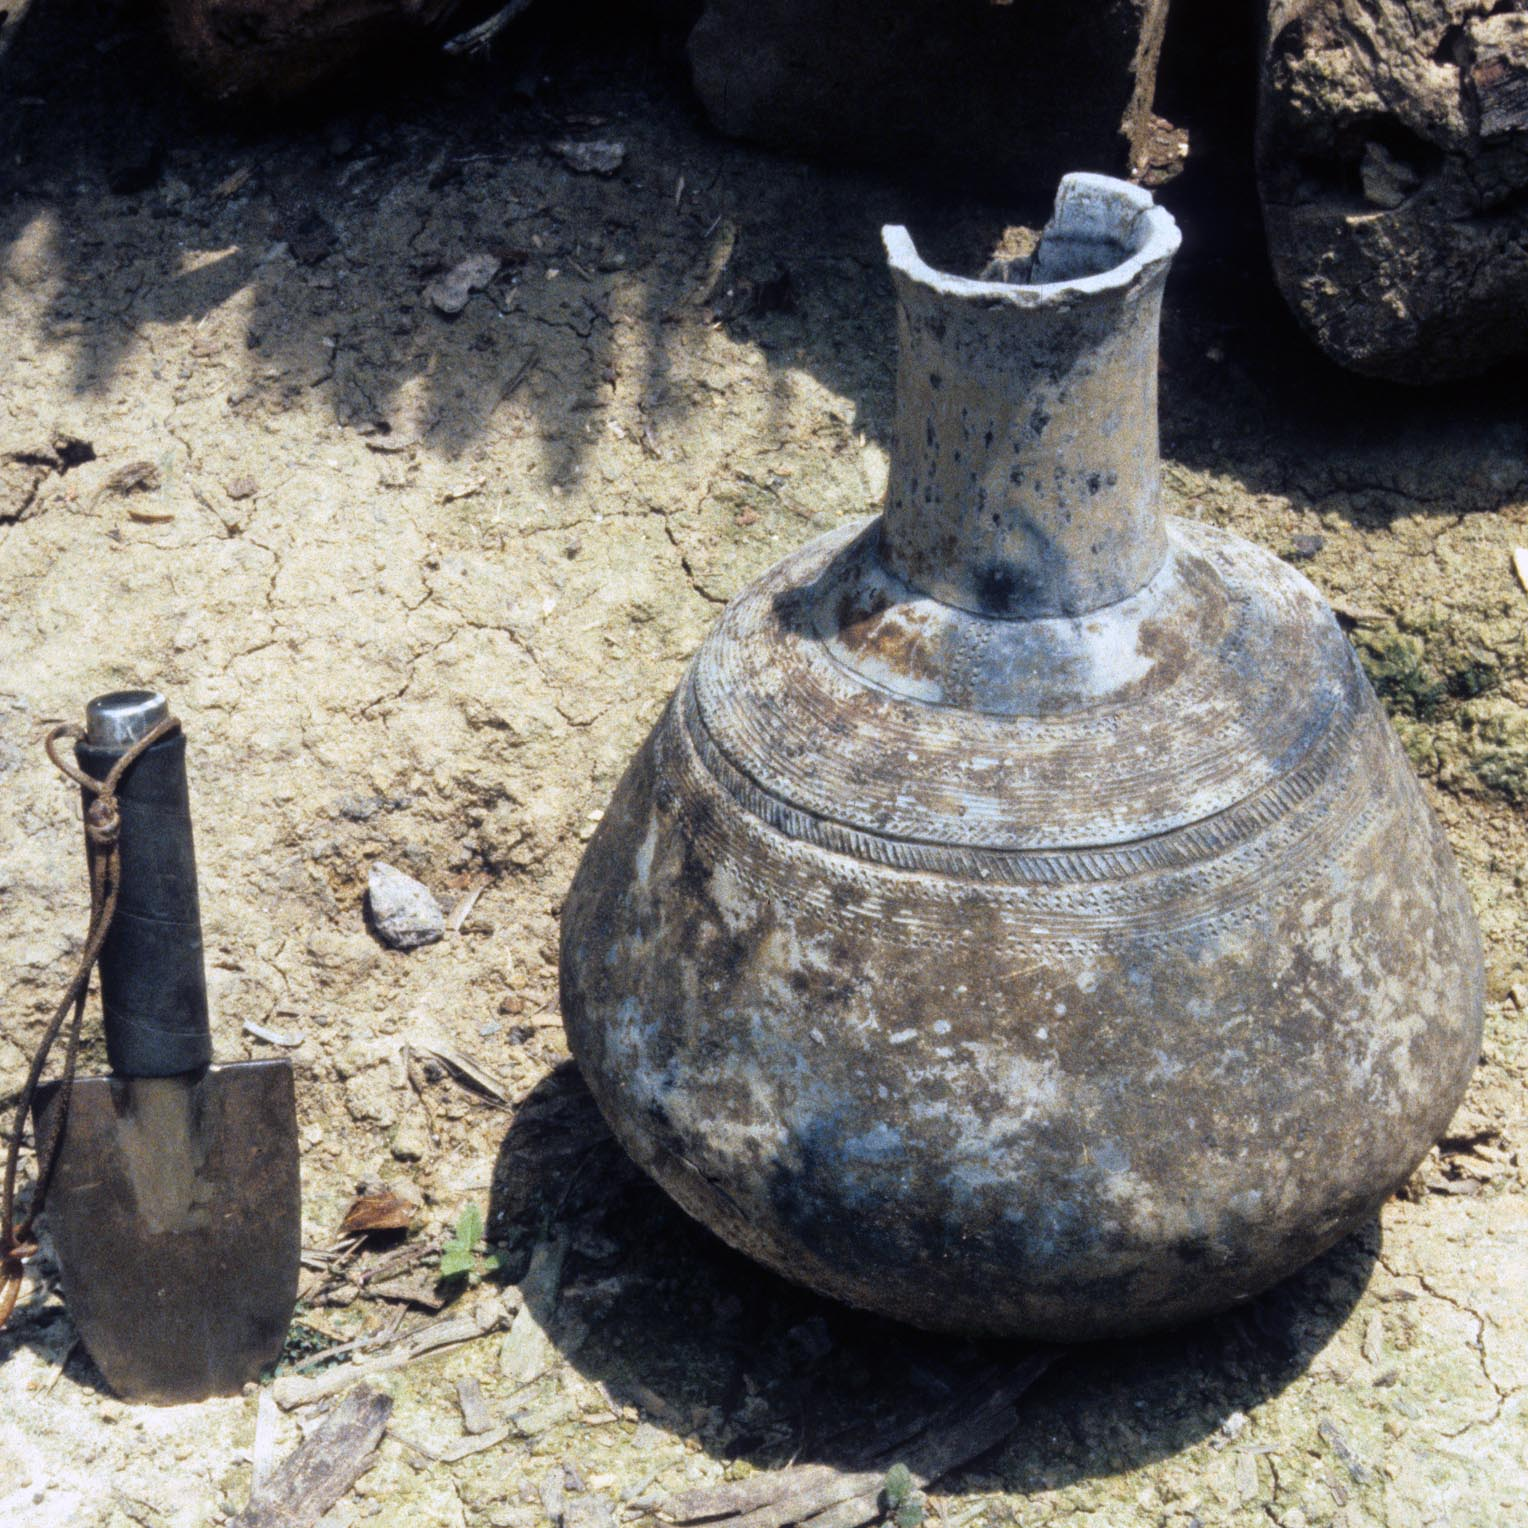
\includegraphics[width=\textwidth]{fig/MUN87-101_E87-036-3.jpg}
	\end{minipage}\hfill
	\begin{minipage}[b]{\columnwidth}
		\caption{Munda (Fpl.~304): Flasche vom Typ A3 (Foto: M.~K.~H. Eggert, 1987).}\label{fig:MUN87-101_EPE-Flasche}
	\end{minipage}
\end{figure*}

Mit Blick auf die Proportionen der Epena-Gefäße sind zwei Gruppen zu unterscheiden: die schalenförmigen Gefäße sind regelhaft etwa doppelt so breit (10--42\,cm) wie hoch (5,5--10\,cm). Da knapp 48\,\% der Schalen der Epena-Gruppe lediglich im Randbereich ließ sich die Mündungshöhe jedoch nur selten rekonstruieren. Bei fast allen hohen Gefäßen mit Schulterabsatz und Kegelhals (B4) ließ sich die Höhe der Mündung nicht ermitteln. Die wenigen GE, die eine Rekonstruktion zuließen, deuten ein Verhältnis zwischen maximalem Durchmesser und Mündungshöhe von 1:1,5 an. Die flaschenförmigen Gefäße vom Typ A3 weisen regelhaft einen großen Bauchdurchmesser auf, der zwischen 10--34\,cm liegt, bei einer Höhe von 11--41\,cm. Die Höhe dieser Gefäße ist häufig nur 20--25\,\% größer als ihr maximaler Durchmesser.

\begin{figure*}[p]
	\centering
	\includegraphics[width=\textwidth]{fig/EPE_Verbreitung.pdf}
	\caption{Epena-Gruppe: Verbreitung.}
	\label{fig:EPE_Verbreitung}
\end{figure*}

Die Ränder der Epena-Gefäße sind entweder ausbiegend (B1; 29\,\%) oder zylindrisch (A1; 28\,\%). Eine sehr spezifische Variante der ausbiegenden Ränder weist einen konvexen Verlauf auf (15\,\%; Taf. 85.4--5, 94.6, 95.4). Es handelt sich hierbei um eine Variante der einfach ausbiegenden, leicht verdickten Ränder des Typs B1, die innerhalb des eng mit der Epema-Gruppe verwandten Ebambe-Stils (Kap.~\ref{sec:EBA-Gr}) regelhaft zu beobachten sind. Kurze sowie lange Varianten ausbiegender Ränder (B1.1--B1.2) konnten bei 6--10\,\% der Randstücke beobachtet werden. Die Randlippen sind zu einem überwiegenden Teil gerade abgestrichen (M3; 66\,\%). Schräg nach innen oder außen abgestrichene Randlippen wurden nur bei jeweils 9--10\,\% der Randstücke beobachtet. Abgerundete sowie spitze Randlippen (M1--2) kommen deutlich seltener, nur bei 4--8\,\% der Randstücke vor.

Bei 31 GE war eine Identifikation des Gefäßbodens möglich. Das Gros dieser GE weist flache Böden auf (74\,\%), wobei die einfachen, flachen Standböden vom Typ B4 mit 65\,\% den Großteil ausmachen. Runde Böden finden sich nur sehr selten im Fundgut der Epena-Gruppe (19\,\%) und ließen sich lediglich bei den sehr selten vorkommenden, flachen Gefäßen mit geschweifter Wandung vom Typ E1 sowie den charakteristischen schalenförmigen Gefäßen mit abknickender Wandung und zylindrischem Oberteil vom Typ G4 beobachten. Alle übrigen Gefäßformen sind regelhaft mit flachen Böden assoziiert (Abb.~\ref{fig:EPE_Typentafel}.1,4--6,10). Böden mit konkaver Standfläche (B6) konnten nur selten beobachtet werden (3\,\%; Abb.~\ref{fig:EPE_Typentafel}.11).

\paragraph{Verzierungen}\hspace{-.5em}|\hspace{.5em}%
Die GE der Epena-Gruppe weisen nur selten Verzierungen auf. Insgesamt 31\,\% aller der Epena-Gruppe zugeordneten GE zeigen kein Dekor und über 75\,\% aller Stücke weisen zwei oder weniger Verzierungselemente auf. Die bestimmenden Verzierungselemente sind Riefen und Rillen, die zusammen 78\,\% ausmachen. Allein horizontale Rillen (Tab.~\ref{tab:Verzierungselemente}: 02.1) machen 47\,\% aller Verzierungselemente aus. Zickzack-Linien (Tab.~\ref{tab:Verzierungselemente}: 01.6; 9\,\%) sowie \textit{Schachbrett}-Muster aus diagonalen Ritzlinien (Tab.~\ref{tab:Verzierungselemente}: 01.2; 8\,\%) stellen innerhalb der Riefen- und Rillen-Verzierungen die häufigsten Verzierungselemente nach den horizontalen Rillen dar. Durch Eindrücke erzielte Verzierungen machen etwa 20\,\% aller Verzierungselemente aus. Eine häufige Variante sind horizontale Reihen aus diagonal gestellten Eindrücken (Tab.~\ref{tab:Verzierungselemente}: 04.12; 10\,\%). Verzierungen beschränken sich auf die Hals- sowie Schulterbereiche der Gefäße (Anlage~4\subref{fig:EPE_Verz}). Insgesamt finden sich etwa 82\,\% aller aufgenommenen Verzierungselemente in diesen beiden Gefäßzonen. Die Standflächen sind regelhaft unverziert.

\paragraph{Datierung}\hspace{-.5em}|\hspace{.5em}%
Für die Epena-Keramik liegen keine absoluten Datierungen vor. Die Keramik wurde bei der Befahrung des Likwala-aus-Herbes 1987 in Benutzung angetroffen, wobei Gefäße fotografisch dokumentiert wurden (Abb.~\ref*{fig:MUN87-101_EPE-Flasche}). Noch in den 1990er Jahren wurde die Herstellung von Gefäßen der Epena-Gruppe in Epena durch \textsc{Mpika-Ngoma} (ebd. 27--36) dokumentiert. Die Epena-Gruppe beschreibt das rezente Spektrum der 1987 genutzten und produzierten Keramik entlang des Likwala-aux-Herbes.

\paragraph{Verbreitung}\hspace{-.5em}|\hspace{.5em}%
Das Verbreitungsgebiet der Epena-Keramik lässt sich im Kern durch den 1987 prospektierten, etwa 500\,km langen Abschnitt des \mbox{Likwala}-\mbox{aux}-\mbox{Herbes} beschreiben (Abb.~\ref*{fig:EPE_Verbreitung}). Entlang der gesamten Strecke fanden sich bei Surveys moderner Dorfflächen GE der Epena-Gruppe. Darüber hinaus fand sich lediglich in Leme (Fpl.~269) am Oberlauf des \mbox{Sangha} ein hohes Gefäß mit weitem und langem Halsbereich sowie stark profilierter Gefäßwandung vom Typ~B2 (Taf.~61.16). Vereinzelt ließ sich Keramik der Epena-Gruppe auch an Fundorten im Mündungsbereich des \mbox{Sangha}, genauer in Bonga (Fpl.~238) sowie Bobusa (Fpl.~239) und in Sungu (Fpl.~236) und Gombe (Fpl.~237) am Kongo nachweisen. Entlang des \mbox{Likwala}-\mbox{aux}-\mbox{Herbes} wurde von der lokalen Bevölkerung angegeben, dass entsprechende Keramik lediglich in Epena am Oberlauf des Flusses (Fpl.~306) produziert würde. Es handelt sich bei der Epena-Keramik mutmaßlich um ein den \mbox{Likwala}-\mbox{aux}-\mbox{Herbes} stromab verhandeltes Produkt der am eponymen Fundort seinerzeit noch betriebenen Töpferei.\footnote{Entsprechende Angaben machte die lokale Bevölkerung in Sosolo (Fpl.~241) am 06.\,05.\,1987 sowie in Ifondo (Fpl.~253) am 11.\,05.\,1987 (Feldbuch M.~K.~H. Eggert 1987).}

\subsubsection{Mobaka-Gruppe}\label{sec:MKA-Gr}

Entlang des \mbox{Likwala}-\mbox{aux}-\mbox{Herbes} sowie des Unterlaufs des \mbox{Sangha} fand sich eine weitere Gruppe rezenter Keramik, welche sich vor allem durch rundbodige Knickwandschalen des Typs F3 auszeichnet. Insgesamt können 79~GE dieser nach der Fundstelle Mobaka am unteren \mbox{Sangha} (Fpl.~246) benannten Stilgruppe zugerechnet werden. Überdies wurden 23 Scherben ausgezählt erfasst. Randscherben, die 80\,\% aller Stücke ausmachen, sind in so großer Zahl im Inventar der Mobaka-Gruppe vertreten, da ausbiegende Ränder mit einem innenseitig scharfen Umbruch eines der wenigen diagnostisches Merkmals der Stilgruppe sind. Daneben fanden sich acht komplette oder hinreichend komplette Gefäße. Einige Wandungsfragmente konnten -- vornehmlich aufgrund ihre Bemalung mit vertikalen, dunklen Streifen -- der Mobaka-Gruppe zugerechnet werden. Die Zuordnung zu dieser Stilgruppe konnte in 70\,\% aller Fälle sicher vorgenommen werden. Funde der Mobaka-Gruppe sind von 21 Fundplätzen bekannt, vor allem entlang des \mbox{Likwala}-\mbox{aux}-\mbox{Herbes} sowie des unteren \mbox{Sangha}. Aus Gombe am Kongo (Fpl.~237) liegen zwei möglicherweise der Mobaka-Gruppe zurechenbare GE vor. Das Gros der Funde stammt aus Yumba (Fpl.~289), Botwale (Fpl.~286), Boleko (Fpl.~292), Misongo (Fpl.~288) sowie Bojenjo (Fpl.~292). Alle diese Fundstellen erbrachten je mindestens zehn GE der Mobaka-Gruppe, wobei sich in Yumba mit 26~GE die meisten Stücke fanden. Die maßgebende Beschreibung der Charakteristika der Mobaka-Gruppe erfolgte jedoch anhand eines kompletten Gefäßes aus der namensgebenden Fundstelle Mobaka am untere \mbox{Sangha} (Fpl.~246; Abb.~\ref{fig:MKA-Typen}.1).


\paragraph{Technologische Merkmale}\hspace{-.5em}|\hspace{.5em}%
Die Keramik der Mobaka-Gruppe wurde in der Regel aus weißbrennenden Tonen hergestellt (65\,\%). Lediglich in wenigen Fällen ließen sich Stücke beobachten, die aus rotbrennenden Tonen gearbeitet sind (12\,\%). Bei einer größeren Anzahl GE (23\,\%) ließ sich aufgrund ihrer beigen, grauen bis schwarzen Färbung die Brennfarbe der Tone nicht sicher ansprechen. Die GE enthalten so gut wie keine (69\,\%) oder nur sehr wenige (22\,\%) nichtplastische Partikel. Sind Partikel sichtbar, so handelt es sich für gewöhnlich um homogene Quarzsande (82\,\%), welche vor allem in der Korngrößenklasse \textit{very fine} (50\,\%) vorliegen. Teilweise finden sich jedoch auch größere Partikel der Größenklassen \textit{fine} (21\,\%), \textit{medium} (24\,\%) sowie vereinzelt auch \textit{coarse} (6\,\%). In nur sehr wenigen Fällen enthalten die Stücke mehr als reine Quarzpartikel: Laterit (11\,\%) oder Organik (4\,\%). Daraus folgt, dass sich das Gros der Mobaka-Keramik dem \textit{Fabric} 1 zurechnen lässt (88\,\%). Die \textit{Fabrics} 1b und 1d machen zusammen zwei Drittel (66\,\%) aller GE der Mobaka-Gruppe aus. In geringem Maße finden sich auch Stücke, welche dem rötlich-brennenden \textit{Fabric} 2 angehören sowie jeweils ein Stück der \textit{Fabrics} 3c und 4a. Die Oberflächen der Stücke sind fast ausschließlich glatt (75\,\%), nur sehr wenige Stücke zeigen eine leicht raue Oberfläche (5\,\%), welche sich aber in jeweils einem der Fälle nur auf die Innen- oder Außenseite beschränkt. Die Dicke der Gefäßwandungen liegt im Mittel bei 6,6\,mm, jedoch wurden auch einige Stücke mit deutlich stärkeren Wandungen beobachtet.

\begin{figure*}[p]
	\centering
	\includegraphics[width=\textwidth]{fig/MKA-Typen.pdf}
	\caption{Mobaka-Gruppe: Typvertreter.\\ 1:~Taf.~39.1; 2:~Taf.~73.3; 3:~Taf.~74.7; 4:~Taf.~68.4 (Reste von Bemalung aus vertikalen, dunklen Streifen wie 1--3, nicht abgebildet); 5:~Taf.~74.8.}
	\label{fig:MKA-Typen}
\end{figure*}

\begin{figure*}[p]
	\centering
	\begin{subfigure}{\columnwidth}
		\centering
		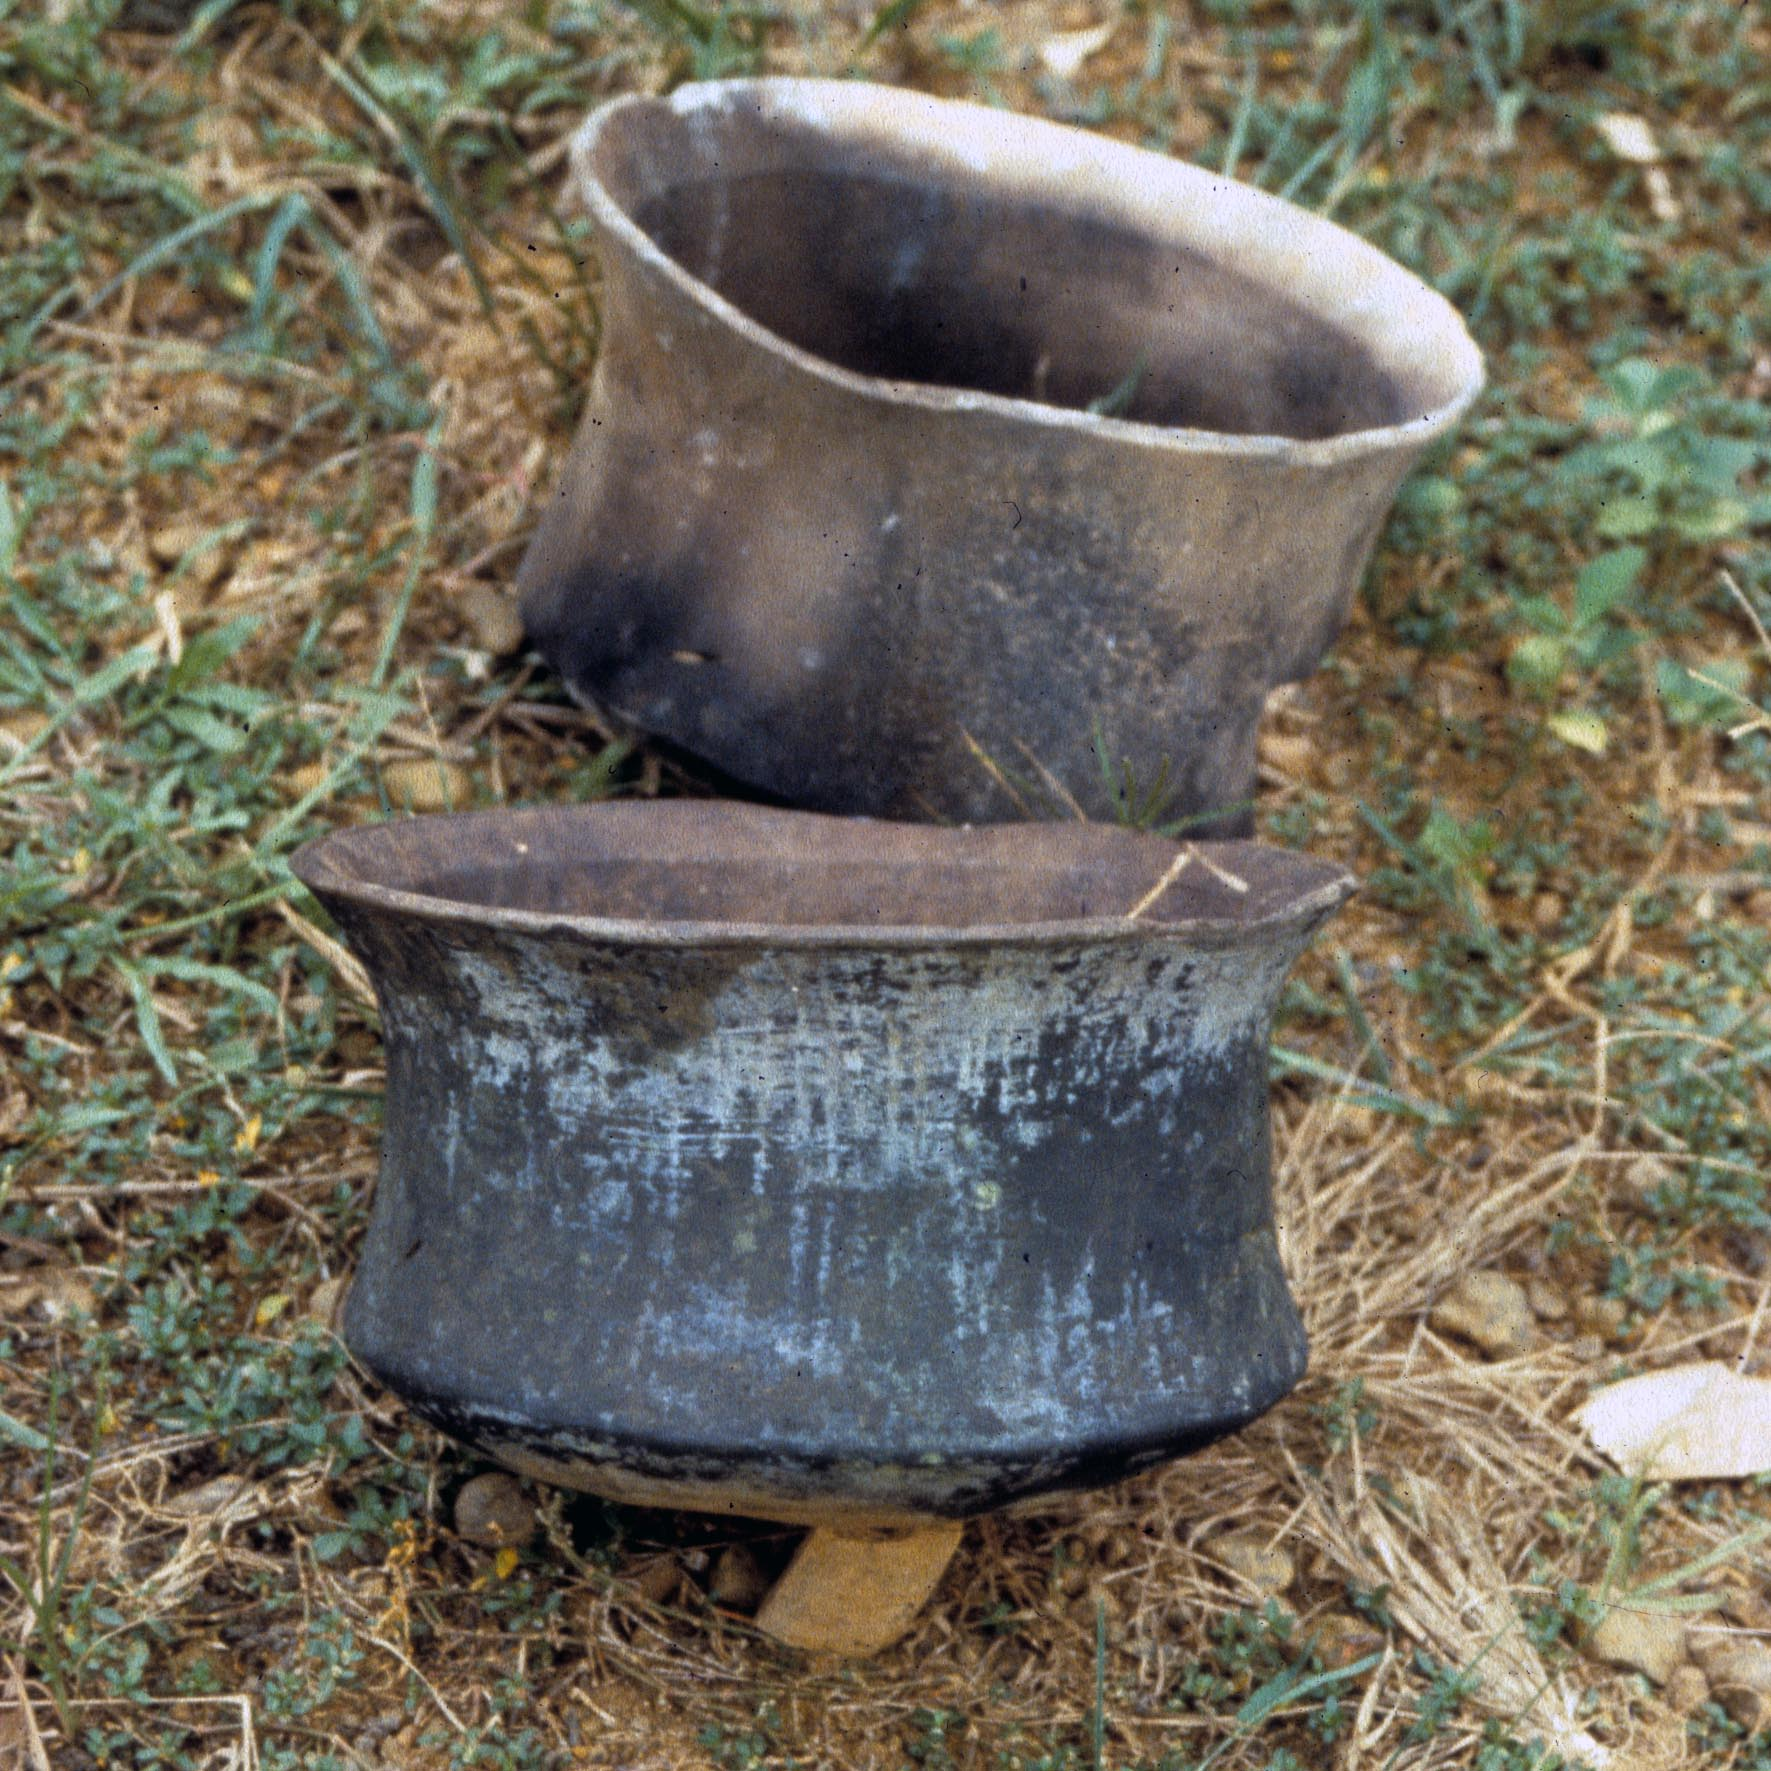
\includegraphics[width = \columnwidth]{fig/BOO87-101_HH87-II-18-27.jpg}
		\caption{Bondo (Fpl.~245; Foto: H.~Holsten, 1987).}
		\label{fig:BOO87-101}
	\end{subfigure}\hfill
	\begin{subfigure}{\columnwidth}
		\centering
		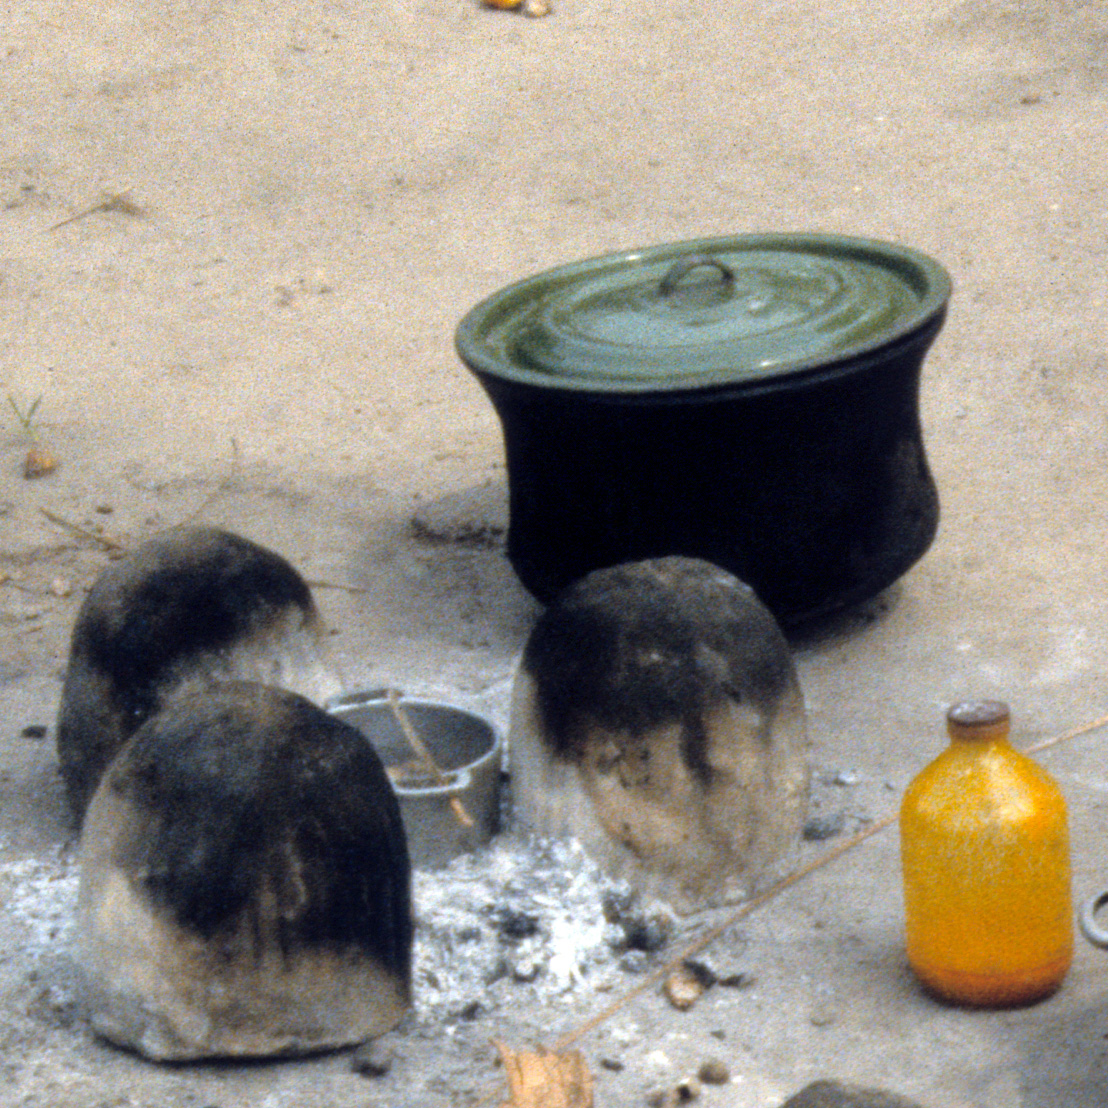
\includegraphics[width = \columnwidth]{fig/MIS87-101_E87-029-14_b.jpg}
		\caption{Misongo (Fpl.~288; Foto: M.~K.~H.~Eggert, 1987).}
		\label{fig:MIS87-101_Detail}
	\end{subfigure}
	\caption{Mobaka-Gruppe: Im Gelände beobachtete, rezente Schalen des Typs F3. Die beiden Gefäße in Bondo am \mbox{Sangha} (Fpl.~245; \textbf{A}) sollen Berichten der lokalen Bevölkerung nach aus Bamataba am \mbox{Sangha} stammen. Eine Fotografie einer Feuerstelle in Misongo am \mbox{Likwala}-\mbox{aux}-\mbox{Herbes} (Fpl.~288; \textbf{B}) zeigt tönerne, zuckerhutförmige Feuerböcke sowie eine Schale des Typs F3 mit Metalldeckel.}
	\label{fig:rezenteMBK-Schalen}
\end{figure*}

\begin{figure*}[p]
	\centering
	\includegraphics[width=\textwidth]{fig/MKA_Verbreitung.pdf}
	\caption{Mobaka-Gruppe: Verbreitung.}
	\label{fig:MKA_Verbreitung}
\end{figure*}

\paragraph{Formen}\hspace{-.5em}|\hspace{.5em}%
Bei insgesamt 22 von 41~GE konnte die Gefäßform sicher bestimmt werden. Bei 33~GE und damit dem überwiegenden Teil handelt es sich um Schalen mit scharfem Bauchknick vom Typ F3 (78\,\%; Abb.~\ref{fig:MKA-Typen}.1--3,5). Die Schalen weisen maximale Durchmesser zwischen 11--32\,cm auf, während die Mündungen zwischen 6--50\,cm weit sind. Die Höhe der Mündung liegt zwischen 6,5--21\,cm. Die sich daraus ergebenden Proportionen der Mündungshöhe zum maximalen Durchmesser, der häufig auch durch den Mündungsdurchmesser gegeben ist, liegt bei zirka 1:1,8. Die Schalen sind folglich häufig fast doppelt so breit wie hoch. Die Bestimmung der Mobaka-Gruppe fußt zu großen Teilen auf den beschriebenen Schalen des Typs F3. Daneben wurden charakteristische Ränder mit innen liegendem scharfen Umbruch sowie die Bemalung mit vertikalen Streifen, welche sich aber nur auf einigen der Schalen findet, für die Zuweisung zur Mobaka-Gruppe herangezogen. Selten konnten andere Gefäßformen der Mobaka-Gruppe zugeordnet werden. So fand sich in Grab BLK~87/1 in Boleko, an der Mündung des \mbox{Likwala}-\mbox{aux}-\mbox{Herbes} (Fpl.~285), ein Gefäß mit geschweifter Wandung und einfach ausbiegendem Rand vom Typ E1, das aufgrund einer äußeren Bemalung mit dunklen, vertikalen Streifen, die ansonsten nur die genannten Schalen der Mobaka-Gruppe zeigen (Abb.~\ref{fig:MKA-Typen}.1--3), der Stilgruppe zugerechnet wird (Abb.~\ref{fig:MKA-Typen}.4). 

Bei 67~GE der Mobaka-Gruppe war der Rand erhalten. Die Mobaka-Gefäße werden von ausbiegenden Formen mit einem innenseitigen scharfen Umbruch bestimmt (B1.5; 77\,\%). Darüber hinaus sind lediglich einfach ausbiegende Ränder vom Typ B1 beobachtet worden. Die Randlippe ließ sich bei insgesamt 58~GE beobachten, sie ist größtenteils schräg nach außen abgestrichen (M5; 67\,\%), in seltenen Fällen aber auch spitz ausgeformt (14\,\%) oder gerade abgestrichen (7\,\%). Die schräg nach außen abgestrichenen Randlippen finden sich regelhaft und fast ausschließlich an den ausbiegenden Rändern mit innenseitigem Profilknick vom Typ B1.5. Aufgrund des Mangels an GE, welche nicht der Schalenform F3 zuzurechnen sind, fehlen GE mit ausgearbeiteten Hals- und Schulterzonen im Inventar der Mobaka-Gruppe vollständig. Die insgesamt 17~GE, bei denen eine Ansprache der Bodenform möglich war, zeigten entweder eine runde Standfläche (B1; 88\,\%) oder einen Linsenboden (B2; 12\,\%). Flache Böden konnten nicht beobachtet werden.

\paragraph{Verzierungen}\hspace{-.5em}|\hspace{.5em}%
Mobaka-Keramik weist häufig nur horizontale Rillen (Tab.~\ref{tab:Verzierungselemente}: 02.1) auf, die knapp die Hälfte aller aufgenommenen Verzierungselemente ausmachen und bis auf wenige Ausnahmen fast durchweg auf der Innenseite der Ränder des Typs B1.5 zu finden sind (Abb.~\ref{fig:MKA-Typen}.1--3,5; Anlage~4\subref{fig:MKA_Verz}). Daneben fallen Bemalungen der Innen- sowie Außenseiten mit vertikalen, dunklen Streifen auf (Tab.~\ref{tab:Verzierungselemente}: 14.1; 26\,\%; Abb.~\ref{fig:MKA-Typen}.1--3). Gelegentlich konnte auch \textit{banfwa-nfwa}-Verzierung auf den Innenseiten sowie außen am Gefäßbauch und den Standflächen beobachtet werden (Tab.~\ref{tab:Verzierungselemente}: 08; 11\,\%; Abb.~\ref{fig:MKA-Typen}.1,5). Die Verzierung findet sich vor allem an der Innenseite der Gefäßränder (52\,\%). Deutlich seltener sind Gefäßwandungen verziert (22\,\%). Bei zwei GE findet sich Verzierung auch auf den Standflächen.

\paragraph{Datierung}\hspace{-.5em}|\hspace{.5em}%
Für die Keramik der Mobaka-Gruppe liegen keine absoluten Datierungen vor, jedoch weisen Fotos entsprechender GE, die während der Prospektionen am \mbox{Sangha} und \mbox{Likwala}-\mbox{aux}-\mbox{Herbes} 1987 gemacht wurden, auf ein rezentes Alter hin (Abb.~\ref{fig:rezenteMBK-Schalen}). Eine rundbodige Schale mit Bauchknick, leicht konkavem Oberteil und vertikaler Bemalung -- die \textit{Leitform} der Mobaka-Gruppe -- aus dem Bereich des Pool Malebo \parencite[150, Taf.~XI.171]{Coart.1907}, findet sich in der umfangreichen Vorlage ethnografischer Funde des \textit{Musée royal de l'Afrique centrale} in Tervuren\footnote{Das Museum trug seinerzeit den Namen \textit{Musée du Congo} (heute \textit{Musée royal de l'Afrique centrale}). Die Gefäße sind als \enquote{Poteries des Bateke, Babuma} beschriftet (\textsc{Anonymus} 1907: Taf. XI).}. Ebenfalls wird eine stark bauchige Flasche aus Kwamouth (ebd. 150, Taf.~XI.172), an der Mündung des Kasai-Flusses in den Kongo, abgebildet, welche eine identische Bemalung zeigt und dem Gefäßtyp A2 entspricht, im hier vorgelegten Material jedoch so nicht beobachtet werden konnte. Eine weitere Schale mit Bauchknick, konkavem Oberteil und gegenständiger Durchlochung unterhalb des Randes, durch die zwei Schnüre gezogen wurden, ist auf einer Fotografie zu sehen, die eine Zusammenstellung von verschiedenen Gefäßen im Tervurener Museum zeigt \parencite[167 Abb. III.11.1]{OmasomboTshonda.2014}. Diese ethnografischen Belege unterstreichen die obengenannte Ansprache der Mobaka-Gruppe als eine rezente Stilgruppe der südlichen Hälfte des Arbeitsgebietes. Basierend auf diesen ethnografischen Belegen kann das früheste Aufkommen entsprechender Formen mindestens für das Ende des 19.~Jh. n.~Chr. angesetzt werden. Ältere Zeugnisse für Mobaka-Keramik sind bisher nicht bekannt.

\paragraph{Verbreitung}\hspace{-.5em}|\hspace{.5em}%
Die Keramik der Mobaka-Gruppe, vor allem die charakteristischen Schalen mit Bauchknick, finden sich entlang des gesamten befahren Abschnitts des \mbox{Likwala}-\mbox{aux}-\mbox{Herbes} sowie am Unterlauf des \mbox{Sangha} (Abb.~\ref{fig:MKA_Verbreitung}). Die nördlichste Fundstelle mit sicheren Funden der Mobaka-Gruppe ist Itanga am \mbox{Likwala}-\mbox{aux}-\mbox{Herbes} (Fpl.~305), während das Verbreitungsgebiet in Richtung Süden bis nach Sosolo an der Mündung des \mbox{Sangha} (Fpl.~241) reicht. Das Verbreitungsgebiet der Mobaka-Keramik weist ein deutliches Kernareal am Unterlauf des \mbox{Likwala}-\mbox{aux}-\mbox{Herbes} zwischen Ngombe (Fpl.~283) und Yumba (Fpl.~289) auf. Basierend auf ethnografischen Belegen \parencite[Taf.~XI.171--172]{Coart.1907} kann das Verbreitungsgebiet der Mobaka-Keramik auch deutlich nach Süden, über das Arbeitsgebiet hinaus, ergänzt werden.

\subsubsection{Mandombe-Gruppe}\label{sec:MDB-Gr}

Die Mandombe-Gruppe beschreibt eine keramische Stilgruppe aus dem Gebiet des oberen \mbox{Sangha} sowie \mbox{Ngoko}, deren Formen und Verzierungen am umfangreichsten in Pikunda am \mbox{Sangha} (Fpl.~255) beobachtet wurden. Die an diesem Platz im Grabungsschnitt PIK~87/1 (Kat.-Nr.~8) in Teilen ausgegrabene Grube A enthielt ein umfangreiches keramisches Inventar, das den Grundstock für die Beschreibung der Stilgruppe bildet.\footnote{Da der Name der Fundstelle Pikunda bereits in der Stilgruppe Pikunda-Munda (Kap.~\ref{sec:PKM-Gr}) Verwendung findet und diese Bezeichnung auch in die Literatur eingegangen ist \parencites{Eggert.1992}{Eggert.1993}{Wotzka.1995}, konnte die hier beschriebene Stilgruppe nicht nach jenem Platz benannt werden. In größerem Umfang fand sich auch am Fundplatz Mandombe am \mbox{Sangha} (Fpl.~259) Keramik dieses Stils und dieser wurde daher als eponyme Fundstelle herangezogen.} Diese Grabung sowie vereinzelte Scherben des Mandombe-Stils in der benachbarten, rezenten Grube PIK~87/2 (Kat.-Nr.~9) lieferten insgesamt 508 individuelle GE, die sich der Mandombe-Gruppe zuweisen lassen. 275~GE aus diesen beiden Grabungen wurden individuell aufgenommen und 233 kleinere Scherben ausgezählt erfasst. Vertreter der Mandombe-Gruppe fanden sich auch in den Oberflächenabsammlungen in Pikunda am \mbox{Sangha} sowie am eponymen Fundplatz Mandombe (Fpl.~259). Von diesen und weiteren Funden aus Surveys wurden 92~GE individuell aufgenommen und 51 weitere, kleinere Scherben ausgezählt erfasst. Insgesamt ließen sich GE von 15 Fundstellen der Mandombe-Gruppe zuweisen (Abb.~\ref{fig:MDB_Verbreitung}). Bestimmendes Charakteristikum der Mandombe-Gruppe sind ihre stark bauchigen Kugeltöpfe mit kurzen zylindrischen Hälsen vom Typ D1 und die auf Riefen, Eindrücken und plastischen Elementen basierende Verzierung sowie eine systematische Schlicker-Rauung der Gefäßunterseiten. Das Fundgut der Mandombe-Gruppe setzt sich vornehmlich aus Wandungsstücken zusammen, die 66\,\% aller aufgenommenen Stücke der Stilgruppe ausmachen. Daneben fanden sich etwa 34\,\% Randfragmente und nur zwei hinreichend vollständige Gefäße (Abb.~\ref{fig:MDB_Typverteter}.1; Taf.~48.2).

\begin{figure*}[!tb]
	\centering
	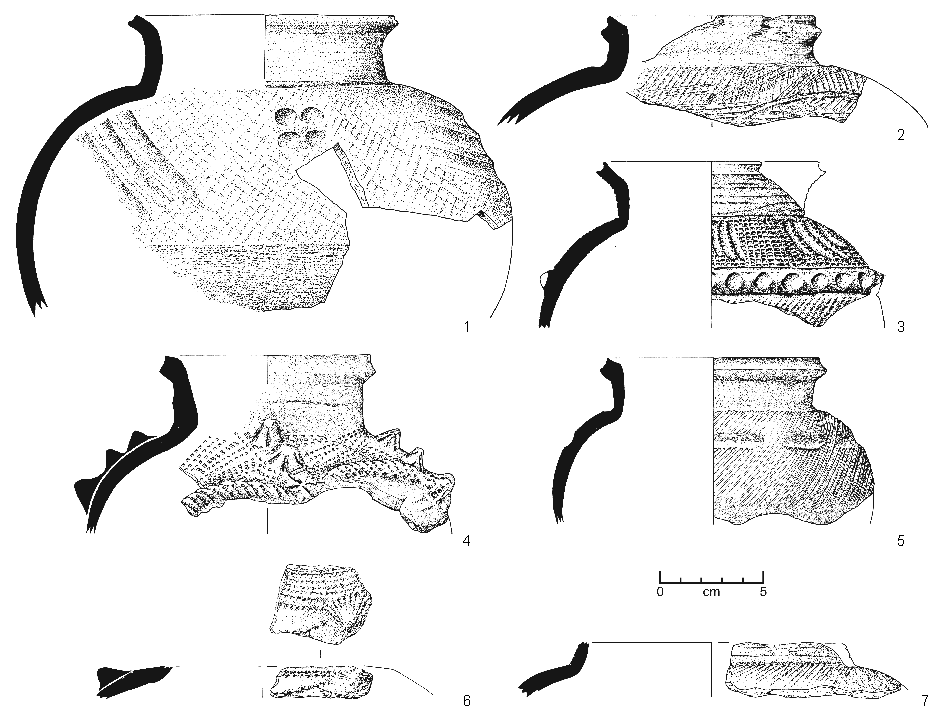
\includegraphics[width=\textwidth]{fig/MDB-Typen.pdf}
	\caption{Mandombe-Gruppe: Typvertreter.\\1:~Taf.~47.24; 2:~Taf.~48.4; 3:~Taf.~55.11; 4:~Taf.~47.23; 5:~Taf.~47.22; 6:~Taf.~57.11; 7:~Taf.~62.6.}
	\label{fig:MDB_Typverteter}
\end{figure*}

\begin{figure*}[!tb]
	\centering
	\begin{subfigure}[t]{.32\textwidth}
		\centering
		
\includegraphics[width = \textwidth, page = 1]{tbl/Tab_Fabrics/x_fabrics_scales.pdf}
		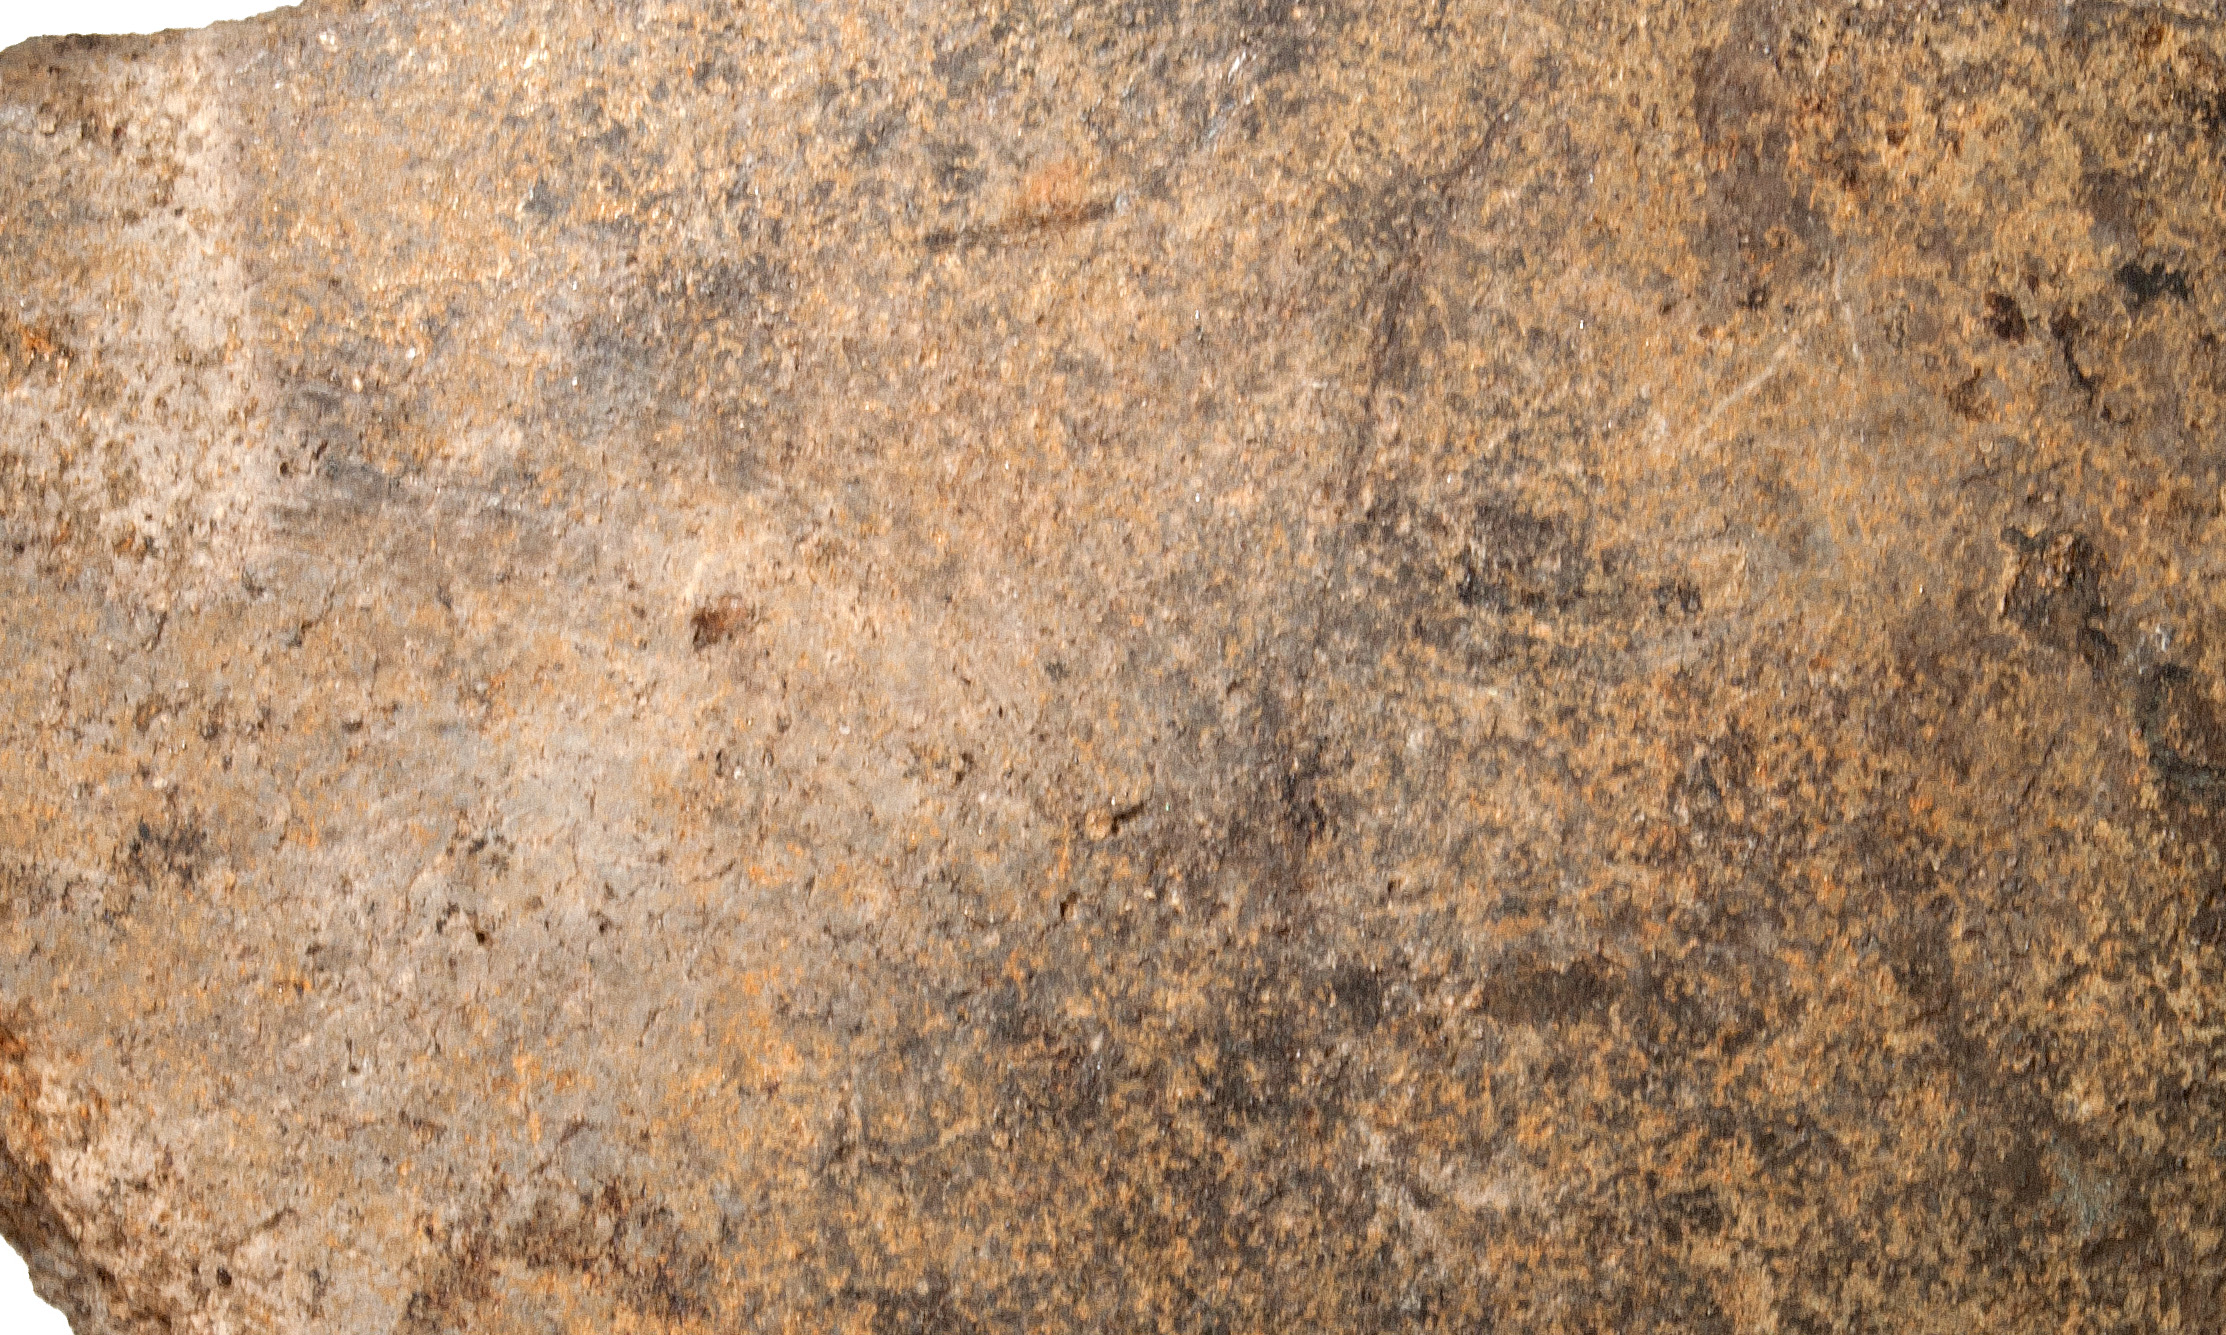
\includegraphics[width = \textwidth]{tbl/Tab_Fabrics/PIK87-2-6-77_outer_5cm.jpg}
		\caption{Außenseite.}
		\label{fig:PIK87-2-6-77_aussen}
	\end{subfigure}\hfill
	\begin{subfigure}[t]{.32\textwidth}
		\centering
		
\includegraphics[width = \textwidth, page = 2]{tbl/Tab_Fabrics/x_fabrics_scales.pdf}
		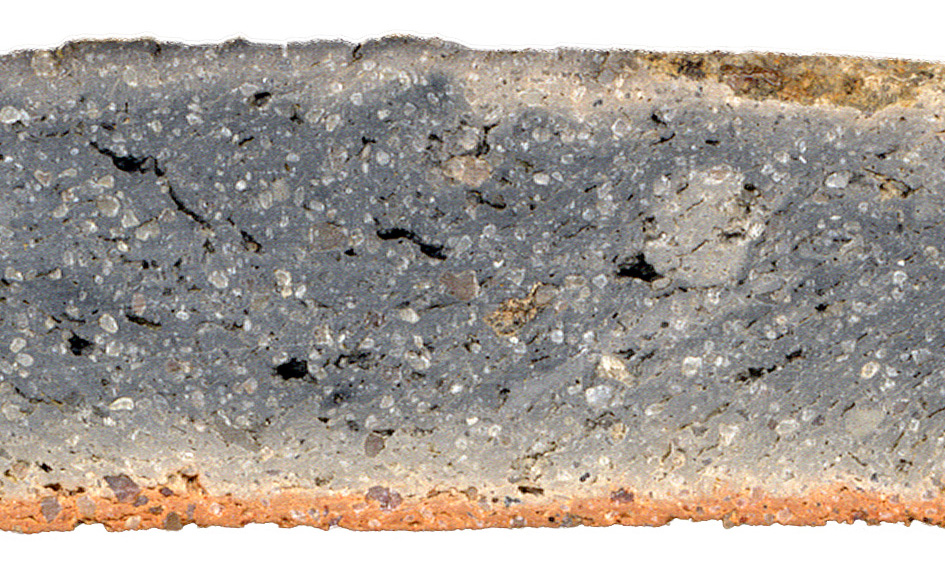
\includegraphics[width = \textwidth]{tbl/Tab_Fabrics/PIK87-2-6-77_2cm.jpg}
		\caption{Profil.}
		\label{fig:PIK87-2-6-77_profil}
	\end{subfigure}\hfill
	\begin{subfigure}[t]{.32\textwidth}
		\centering
		\includegraphics[width = \textwidth, page = 1]{tbl/Tab_Fabrics/x_fabrics_scales.pdf}
		\includegraphics[width = \textwidth]{tbl/Tab_Fabrics/PIK87-2-6-77_inner_5cm.jpg}
		\caption{Innenseite.}
		\label{fig:PIK87-2-6-77_innen}
	\end{subfigure} %
	\caption{Mandombe-Gruppe: Scherbe eines aus einem weißbrennenden Ton getöpfertes Gefäß mit innenseitig aus rotbrennendem Ton bestehendem Schlicker (\textbf{B}--\textbf{C}; Kat.-Nr.~9).}
	\label{fig:PIK87-2-6-77}
\end{figure*}

\paragraph{Technologische Merkmale}\hspace{-.5em}|\hspace{.5em}%
Mandombe-Keramik zeichnet sich durch hohe Anteile nichtplastischer Partikel aus. 68\,\% aller GE weisen mehr als 15--20\,\% nichtplastische Partikel im Scherben auf, die vornehmlich den Größenklassen \textit{medium} (33\,\%) bis \textit{coarse} (55\,\%) zuzurechnen sind. Es handelt sich größtenteils (60\,\%) um feinen, heterogenen Quarzsand sowie ausgebrannte Organik (siehe Abb.~\ref{PIK87-1-2-3_1-3-7_Makrospuren}). Selten finden sich auch Glimmer oder lateritähnliche Partikel. Zusammengenommen 88\,\% der Scherben lassen sich einem \textit{Fabric} der Gruppe 3 zuweisen, wobei 50\,\% auf die Variante 3a, 26\,\% auf die Variante 3b und 3\,\% auf die Variante 3c entfallen. Weitere 21\,\% ließen sich nicht genau einer Variante zuordnen.\footnote{Auch die bei ihrer Herstellung 1987 in Pikunda beobachteten Gefäße weisen einen Scherben auf, der dem \textit{Fabric} 3 entspricht. Damit lassen sich Rückschlüsse auf Rohmaterialgewinnung und Rohmaterialaufbereitung sowie den Brand der Gefäße der Mandombe-Gruppe ziehen. Siehe Anm.~\ref{ftn:EthnoToepfereiInVorb}.} Neben \textit{Fabrics} des Typs 3 finden sich in sehr geringen Anteilen Stücke, die einzelnen Varietäten der \textit{Fabrics} 4--8 zuordenbar sind. Die Brennfarbe lässt sich, aufgrund grauer bis beiger Farbtöne, für etwa 45\,\% aller Stücke nicht hinreichend genau bestimmen. Stücke, deren Färbung auf die Nutzung rotbrennender Tone hindeuten, machen 31\,\% aus, während solche, die weißbrennende Tone anzeigen, etwa 23\,\% ausmachen. Die Oberflächen der Stücke sind geglättet (69\,\%) oder leicht rau (22\,\%). Die Dicke der Gefäßwandungen liegt im arithmetischen Mittel bei 6,9\,mm, mit einer Varianz von 3,7\,mm.

Charakteristisch ist der zwar hohe Anteil nichtplastischer Partikel, jedoch auch die Begrenzung auf Partikel der Größenklassen \textit{medium} bis \textit{coarse}. Gerade innerhalb einer GE schwankt die Korngröße der nichtplastischen Partikel nur wenig und man gewinnt den Eindruck, das Korngrößenspektrum sei künstlich eingegrenzt worden, zum Beispiel durch Sieben. Die zweite wichtige technische Eigenheit der Mandombe-Keramik betrifft die beobachtbaren Auswirkungen des Brandes auf die Färbung der Stücke. Fast alle Stücke, wiederum auch ein bestimmendes Merkmal der \textit{Fabrics} vom Typ 3, zeigen lediglich eine randliche, deutlich von einem homogen grauen Kern abgegrenzte Oxidation (Abb.~\ref{fig:PIK87-2-6-77_profil}).\footnote{Neben diesen Charakteristika der Mandombe-Keramik fand sich im Fundgut der rezenten Grube PIK~87/2 in Pikunda am \mbox{Sangha} (Kat.-Nr.~9; Fpl.~255) eine GE, die auf ihrer Innenseite einen zusätzlichen Auftrag aufweist. Das aus weißbrennendem Ton aufgebaute Gefäß zeigt innen eine deutlich abgrenzbare, rote Lage (Abb.~\ref{fig:PIK87-2-6-77}).}

\begin{figure*}[p]
	\centering
	\includegraphics[width=\textwidth]{fig/MDB_Verbreitung.pdf}
	\caption{Mandombe-Gruppe: Verbreitung \parencite[P1 nach][114 Abb.~42]{Gillet.2013}.}
	\label{fig:MDB_Verbreitung}
\end{figure*}

\paragraph{Formen}\hspace{-.5em}|\hspace{.5em}%
Das Formenspektrum der Mandombe-Gruppe ist sehr homogen. Während bei insgesamt 119~GE die Gefäßform angesprochen werden konnte, war die Bestimmung nur bei etwas über der Hälfte dieser Stücke hinreichend zuverlässig möglich. Insgesamt 87\,\% aller Formen machen Gefäße mit stark konvexer Wandung und ohne ausgeprägten Halsbereich aus (Abb.~\ref{fig:MDB_Typverteter}), wobei sichere und fragliche Ansprachen zu etwa gleichen Teilen vorkommen.\footnote{Die maximalen Durchmesser dieser Gefäße schwanken zwischen zwölf und 32\,cm. Die aufgenommenen Durchmesser an den verschiedenen Gefäßpositionen wie Mündung, minimaler Halsdurchmesser sowie maximaler Bauchdurchmesser (Abb.~\ref{fig:GefAbmessungen_Schema}) zeigen jeweils mehr oder weniger eingipfelige Verteilungen und lassen keine konkreten Größenklassen erkennen, die eine weitere Untergliederung rechtfertigen könnten. Während die Messungen der Durchmesser an der Gefäßmündung sowie der minimale Durchmesser im Halsbereich jeweils einer eingipfeligen Normalverteilung entspricht, streut die Verteilung für den maximalen Bauchdurchmesser stärker. Die Höhen der Mündung (Abb.~\ref{fig:GefAbmessungen_Schema}) konnten -- da kein Gefäß hinreichend erhalten war -- bei keiner GE ermittelt werden. Rekonstruiert man jedoch die stark kugelige Form der Gefäße und projiziert entsprechend runde Böden, so müssten die Höhen der Gefäße in etwa bei Werten um die entsprechenden maximalen Durchmesser gelegen haben.} Das Spektrum an Randformen der Mandombe-Gruppe wird von ausbiegenden Rändern bestimmt. Das Gros bilden kurze, einfach ausbiegende Formen vom Typ B1.1. Diese machen knapp die Hälfte aller 120 aufgenommenen Ränder aus. Zahlreich kommen noch konkav (B2; 29\,\%) sowie gerade ausbiegende Ränder (B1; 12\,\%) vor. Die Randlippen weisen regelhaft eine Rille auf (M4; 90\,\%; Abb.~\ref{fig:MDB_Typverteter}.1--5). Die Halspartien der Gefäße sind zu 91\,\% kurz und überwiegend zylindrisch (31\,\%) oder konkav (33\,\%) ausgeführt. In einigen Fällen verläuft auf dem Gefäßhals ein horizontaler Wulst (Abb.~\ref{fig:MDB_Typverteter}.2, 4). Die Gefäßschultern sind überwiegend deutlich konvex (72\,\%). Die Ausprägung des Gefäßbodens konnte bei keiner der sicher der Mandombe-Gruppe zugerechneten GE beobachtet werden. Zwei nicht zweifelsfrei der Stilgruppe zugehörige GE zeigen runde Böden (B1--B2), während drei weitere Stücke auf flache (B4) oder profiliert abgesetzte Flachböden (B9--10) hindeuten. Eine spezifische Bodenform ließ sich der Mandombe-Gruppe nicht zuweisen.

\paragraph{Verzierungen}\hspace{-.5em}|\hspace{.5em}%
Das Spektrum an Verzierungen innerhalb der Mandombe-Gruppe wird von diagonalem (Tab.~\ref{tab:Verzierungselemente}: 15.1; 21\,\%) oder überkreuztem Kammstrich (Tab.~\ref{tab:Verzierungselemente}: 15.2; 8\,\%), mehr als 5\,mm breite Riefen (Tab.~\ref{tab:Verzierungselemente}: 02.7; 14\,\%) sowie einfachen horizontalen Riefen (Tab.~\ref{tab:Verzierungselemente}: 02.1; 14\,\%) bestimmt. Der Kammstrich besteht häufig aus Riefen mit kantigem, u-förmigem Profil und findet sich vornehmlich im Schulterbereich sowie auf dem Gefäßbauch (Anlage~4\subref{fig:MDB_Verz}). Auch die breiten Riefen finden sich vornehmlich in diesen beiden Gefäßregionen, während die horizontalen Rillen größtenteils im Hals- sowie Schulterbereich der Gefäße beobachtet wurden. Seltener, jedoch um so charakteristischer sind plastische Elemente wie Knubben (Tab.~\ref{tab:Verzierungselemente}: 09.1; 6\,\%) und Leisten (Tab.~\ref{tab:Verzierungselemente}: 09.2; 2\,\%). Auch sie sind vornehmlich auf dem Schulterbereich der Gefäße zu finden. Die Gefäßunterseiten sind regelhaft unverziert, weisen aber, sofern diese Partie erhalten ist, häufig eine Schlicker-Rauung auf (Abb.~\ref{fig:MDB_Typverteter}.1). Grundsätzlich finden sich über die Hälfte aller aufgenommenen Verzierungselemente (55\,\%) im Bereich der Gefäßschulter, gefolgt vom Bauchbereich (27\,\%). Die Ränder sind innen wie außen nur selten verziert, ähnlich der Gefäßhälse.

Lediglich drei zweifelsfrei der Mandombe-Gruppe zuordenbare Randscherben aus dem Survey in Pikunda am \mbox{Sangha} (Fpl.~255) weisen \textit{knotted string}-\mbox{Roulette} (Tab.~\ref{tab:Verzierungselemente}: 21.1) im Schulterbereich auf. In allen Fällen wird das \mbox{Roulette} von breiten Reifen überlagert (Taf.~55.12) sowie von Knubben oder plastischen Leisten begleitet. Die starke Ähnlichkeiten zur Mandombe-Keramik aufweisende Konda-Gruppe (Kap.~\ref{sec:KON-Gr}) zeigt ebenfalls ein auf Einzelstücke begrenztes Auftreten von Rouletteverzierung.

\paragraph{Datierung}\hspace{-.5em}|\hspace{.5em}%
Für die Keramik der Mandombe-Gruppe liegt eine Radiokohlenstoffdatierung aus der im Grabungsschnitt PIK~87/1 (Kat.-Nr.~8) in Pikunda am \mbox{Sangha} (Fpl.~255) erfassten Grube A vor. Sie datiert demnach in das 13.--15.~Jh. n.~Chr. (Tab.~\ref{tab:PIK87-1_Datierungen}: KI-2891).\footnote{Die benachbarte Grube PIK~87/2 (Kat.-Nr.~9) enthielt ebenfalls keramisches Material, welches der Mandombe-Gruppe zugerechnet beziehungsweise nicht sicher abgegrenzt werden kann. Grundsätzlich muss der Befund jedoch als rezent angesehen werden, wie der Fund eines Plastik-Kamms zeigt. Die Mandombe-Keramik ist mit hoher Wahrscheinlichkeit mit dem Verfüllungsmaterial in die rezente Grube gelangt. Auffällig ist, dass die entsprechende Keramik aus dem Befund PIK~87/2 Rouletteverzierung aufweist, sich ansonsten aber nicht vom Material der Grube A in PIK~87/1 unterscheidet. Ob dies eine sukzessive Integration von Rouletteverzierung in das Verzierungs-Spektrum der Mandombe-Gruppe anzeigt, muss beim gegenwärtigen Stand der Feldarbeiten offenbleiben.}

\paragraph{Verbreitung}\hspace{-.5em}|\hspace{.5em}%
Keramik der Mandombe-Gruppe findet sich fast ausschließlich im Bereich des oberen \mbox{Sangha} sowie an zwei Fundstellen entlang des \mbox{Ngoko} (Abb.~\ref{fig:MDB_Verbreitung}).\footnote{Potenziell der Mandombe-Gruppe zurechenbare Stücke wurden auch in Mboua Mboua am oberen \mbox{Sangha} gefunden \parencite[114 Abb.~42]{Gillet.2013}. Siehe auch Kap.~\ref{sec:PKM-Gr}.} Der südlichste Fundpunkt der Verbreitung und die mit Blick auf die absolut vorliegenden Fundanteile bestimmende Fundstelle ist Pikunda am mittleren \mbox{Sangha} (Fpl.~255). Im Norden, stromauf des \mbox{Sangha}, sowie möglicherweise entlang des \mbox{Ngoko} im Westen, ist die Grenze des Verbreitungsgebietes der Mandombe-Gruppe nicht erfasst und wird lediglich durch die Grenzen des Arbeitsgebietes bestimmt. Gerade die ungleiche Verteilung von aus Pikunda stammenden Grabungsfunden gegenüber deutlich selteneren Surveyfunden erschwert eine stichhaltige Interpretation des Verbreitungsgebietes der Mandombe-Keramik. 

\begin{figure*}[tb]
	\centering
	\includegraphics[width=.95\textwidth]{fig/KON-Typen.pdf}
	\caption{Konda-Gruppe: Typvertreter.\\1:~Taf.~61.1; 2~Taf.~61.2; 3:~Taf.~66.16; 4:~Taf.~61.4; 5:~Taf.~66.9; 6:~Taf.~66.19; 7:~Taf.~66.18.; 8:~Taf.~57.22; 9:~Taf.~60.24; 10:~Taf.~63.12.}
	\label{fig:KON_Typvertreter}
\end{figure*}

\subsubsection{Konda-Gruppe}\label{sec:KON-Gr}

Neben der Keramik der Mandombe-Gruppe (Kap.~\ref{sec:MDB-Gr}) sowie der noch zu beschreibenden Pandama-Keramik (Kap.~\ref{sec:PDM-Gr}) ließ sich eine weitere, vornehmlich am oberen \mbox{Sangha} sowie dem \mbox{Ngoko} verbreitete, keramische Stilgruppe herausarbeiten. Diese, nach dem Fundplatz Konda am oberen \mbox{Sangha} (Fpl.~268) benannte Gruppe, zeichnet sich durch Gefäße mit geschweiftem Profil und konkav ausbiegenden, häufig außen wie innen mit Rillen verzierten Rändern aus (Abb.~\ref{fig:KON_Typvertreter}). Überdies konnten eine große Anzahl kleiner, rundbodiger Schalen beobachtet werden, deren Verzierung sich in das Schema der größeren Gefäße einpasst und die in der Folge ebenfalls der Konda-Gruppe zugerechnet wurden.\footnote{Eine größere Anzahl vergleichbarer Schalen wurde in den späten 1990er Jahren bei Prospektionen im Südosten der Republik Kamerun, die als Fortsetzung des \textit{River Reconnaissance Project} unter der Leitung von Manfred~K.~H. Eggert durchgeführt wurden, entdeckt. Eine eingehende Auswertung dieser Feldarbeiten liegt bislang nicht vor. Grundsätzlich vergleichbare Formen finden sich auch im Fundmaterial des Inneren Kongobeckens. Während ein Stück aus Mbandaka \parencite[Fpl.~10, ][445 Taf. 11.3]{Wotzka.1995} der Bondongo- oder Mbandaka-Gruppe zugeordnet wird (ebd. 426), ist ein weiteres aus Nkile am Ruki (Fpl.~17; ebd. 465 Taf. 31.2--3 der Botendo-Gruppe zuzurechnen (ebd. 428).\label{ftn:KON-PDM_klSchalen}} 

Insgesamt können 156~GE aus 21 verschiedenen Fundplätzen der Kondo-Gruppe zugewiesen werden. Das Material stammt zu 97\,\% aus Absammlungen von Oberflächenkomplexen. Einzelne GE des Konda-Stils wurden in den drei in Pikunda am \mbox{Sangha} (Fpl.~255) ausgegrabenen Befunden (Kat.-Nr.~8--10) sowie in der Grube MUN~87/1 (Kat.-Nr.~15) in Munda am \mbox{Likwala}-\mbox{aux}-\mbox{Herbes} (Fpl.~304) erfasst. Die erste Beschreibung der Konda-Keramik erfolgte größtenteils an Randstücken. Sie machen mit 107~GE (70\,\%) auch das Gros dieser Stilgruppe aus. Ein nahezu vollständiges Gefäß, eine kleine Schale (Taf.~60.24) sowie 47 Fragmente von Gefäßwandungen (30\,\%) bilden den Rest der die Stilgruppe repräsentierenden GE. Bodenstücke sind nicht beobachtet worden. Das Material setzt sich größtenteils aus stark fragmentierten Stücken zusammen. Insgesamt 85\,\% aller Stücke sind kleiner als 70$\times$70\,mm und lediglich eine GE ist größer als 120$\times$120\,mm.


\paragraph{Technologische Merkmale}\hspace{-.5em}|\hspace{.5em}%
Die Scherben der Konda-Gruppe zeichnen sich durch einen deutlichen Anteil nichtplastischer Partikel aus. Über 90\,\% aller Stücke enthalten 25--40\,\% nichtplastische Partikel. Nur in geringem Umfang kommen auch Stücke mit unter 5\,\% Anteil nichtplastischer Partikel im Scherben vor. Die beobachteten Partikel sind fast ausschließlich den Größenklassen \textit{medium} (24\,\%), \textit{coarse} (54\,\%) sowie \textit{very coarse} (19\,\%) zuzurechnen. Es handelt sich vor allem um Quarzsand (77\,\%), der teilweise mit Laterit, Glimmer, Organik oder auch Schamott-Partikeln durchmischt ist. Das Gros ist den \textit{Fabrics} 3 (56\,\%) sowie 4 (27\,\%) zuzurechnen. Mit jeweils weniger als 6\,\% sind die \textit{Fabrics} 5, 7 und 8 vertreten. Mit Blick auf die Brennfarbe des genutzten Tones lassen sich, aufgrund beiger oder grauer Farbe, für 44\,\% der Stücke keine Angaben machen. Stücke, die auf die Nutzung rotbrennender Tone hindeuten, sind mit 26\,\% nur etwas seltener vertreten als solche, die weißbrennende Tone anzeigen. Diese machen 30\,\% aller GE der Konda-Gruppe aus. Die Oberflächen der Scherben sind sehr häufig leicht rau (55\,\%) oder rau (24\,\%).

\begin{figure*}[p]
	\centering
	\includegraphics[width=\textwidth]{fig/KON_Verbreitung.pdf}
	\caption{Konda-Gruppe: Verbreitung \parencite[grau nach][510 Abb.~3]{Eggert.2002}.}
	\label{fig:KON_Verbreitung}
\end{figure*}

\paragraph{Formen}\hspace{-.5em}|\hspace{.5em}%
Bei insgesamt 66~GE der Konda-Gruppe konnte die Gefäßform bestimmt werden, wobei für 21\,\% die Ansprache aufgrund schlechter Erhaltung nur unter Vorbehalt erfolgte. Gefäße mit stark konvexer Wandung, ohne ausgeprägten Halsbereich und konkav ausbiegendem Rand vom Typ D1 machen 33\,\% der beobachteten Formen aus (Abb.~\ref{fig:KON_Typvertreter}.2--7). Die Gefäße weisen maximale Bauchdurchmesser zwischen 12--27\,cm auf, jedoch konnte die Höhe der Mündung bei keiner GE hinreichend rekonstruiert werden. Neben der Gefäßform zeichnen sich diese GE durch einen konkaven, kurzen Gefäßhals aus, der direkt in einen konkav ausbiegenden Rand übergeht und innen wie außen mit horizontalen Rillen verziert ist. Diese Kombination aus Gefäßform, Randgestaltung und Verzierung ist maßgeblich für die Zuordnung von GE zur Konda-Gruppe. Die Konda-Gruppe zeichnet sich überdies durch das zahlreiche Auftreten zumeist kleiner, rundbodiger Schalen mit häufig T-förmig umgelegten Rändern aus (Abb.~\ref{fig:KON_Typvertreter}.8--10). Diese machen insgesamt 48\,\% aller der Konda-Gruppe zugerechneten GE aus. Sie weisen Durchmesser zwischen 12--27~cm auf und sind zwischen 1,5--11,5\,cm hoch. Die Ränder dieser Schalen sind entweder nur nach außen oder T-förmig, nach innen wie außen umgelegt. Ansprachen zum Gefäßboden ließen sich ausschließlich bei diesen Schalen machen und es wurden nur runde Böden beobachtet. In einem Fall konnte eine GE als Flasche identifiziert werden (Abb.~\ref{fig:KON_Typvertreter}.1). Dieses Stück entspricht, bis auf den stark verengten Gefäßhals, den Gefäßen mit konvexer Wandung vom Typ D1 der Konda-Gruppe.


\paragraph{Verzierungen}\hspace{-.5em}|\hspace{.5em}%
Bestimmendes Merkmal der Konda-Keramik ist der hohe Anteil an horizontalen Rillen (Tab.~\ref{tab:Verzierungselemente}: 02.1; 69\,\%), die sich fast ausschließlich innen wie außen am Rand sowie dem Gefäßhals befinden (Anlage~4\subref{fig:KON_Verz}). Daneben weist die Keramik -- deutlich seltener -- horizontale Reihen aus diagonalen (Tab.~\ref{tab:Verzierungselemente}: 04.12; 5\,\%), vertikal stehenden (Tab.~\ref{tab:Verzierungselemente}: 04.15; 5\,\%) oder runden Eindrücken (Tab.~\ref{tab:Verzierungselemente}: 04.11; 2\,\%) sowie diagonalen Kammstrich auf (Tab.~\ref{tab:Verzierungselemente}: 15.1; 4\,\%). Sechs GE sind zudem mit vegetabilischem \mbox{Roulette} verziert, in fünf Fällen handelt es sich um \textit{knotted string}- (Tab.~\ref{tab:Verzierungselemente}: 21.1; Abb.~\ref{fig:KON_Typvertreter}.7) und in einem Fall um \textit{twisted string}-\mbox{Roulette} (Tab.~\ref{tab:Verzierungselemente}: 21.2). Die Rouletteverzierung findet sich in allen Fällen auf dem Gefäßbauch oder der Schulter und tritt immer in Kombination mit anderen Verzierungselementen auf (Anlage~4\subref{fig:KON_Verz}). Trotz des Vorkommens von \mbox{Roulette} wird die Verzierung der Konda-Keramik vor allem von innen wie außen an Rand und Hals der Gefäße zu findenden Riefen und Rillen bestimmt.

\paragraph{Datierung}\hspace{-.5em}|\hspace{.5em}%
Für die Keramik der Konda-Gruppe liegen keine direkten Radiokohlenstoffdatierungen vor. Unter Vorbehalt der Konda-Gruppe zurechenbare GE wurden in allen drei Grabungsschnitten in Pikunda am mittleren \mbox{Sangha} (Fpl.~255) erfasst. Während das Inventar der rezenten Grube PIK~87/2 (Kat.-Nr.~9) eindeutig vermischt ist und die Fundzusammenhänge durch das Fehlen der Dokumentation des als PIK~87/3 (Kat.-Nr.~10) ausgegrabenen Metallurgiebefundes\footnote{Eine Datierung weist diesen Befund grob in das 11.--13.~Jh. n.~Chr. (KI-2892).} nicht mehr zweifelsfrei belegbar sind, liefern lediglich die Einzelfunde aus der jüngeren Grube A in PIK~87/1 (Kat.-Nr.~8) einen Datierungsansatz. Das vornehmlich durch die Keramik der Mandombe-Gruppe (Kap.~\ref{sec:MDB-Gr}) charakterisierte Inventar datiert in das 13.--15.~Jh. n.~Chr. (KI-2891). Diese Datierung deutet zumindest eine partielle Gleichzeitigkeit mit der Keramik der Mandombe-Gruppe an. Das Auftreten von Rouletteverzierung, die in größerem Umfang erst mit der mutmaßlich jüngeren Pandama-Gruppe (Kap.~\ref{sec:PDM-Gr}) aufkommt, deutet hingegen auf ein tendenziell jüngeres Alter im Vergleich zur Mandombe-Keramik. Die grundsätzliche Morphologie der Gefäße und vor allem  die rillenverzierten Gefäßhälse und Ränder deuten einen losen Bezug zur Keramik der Bobulu-Gruppe (Kap.~\ref{sec:BBL-Gr}) des \mbox{Ubangi}-Gebiets an.

\paragraph{Verbreitung}\hspace{-.5em}|\hspace{.5em}%
Die Verbreitung der Konda-Gruppe beschränkt sich auf einen eng begrenzten Bereich entlang des Oberlaufs des \mbox{Sangha} sowie des prospektierten Abschnitts des \mbox{Ngoko} (Abb.~\ref{fig:KON_Verbreitung}).\footnote{Ähnliche, bislang unveröffentlichte Stücke fanden sich auch bei der Wiederaufnahme der Feldarbeiten durch Manfred~K.~H.~Eggert im Südosten der Republik Kamerun in den späten 1990er Jahren \parencite[siehe][]{Eggert.2002} in Mokounounou (Obj. MKN~97/1:15 ) und Tala-Tala (Obj. TLT~97/101:71). Zur Zeit der Materialaufnahme für diese Arbeit war diese kamerunische Keramik in Tübingen eingelagert und nur eingeschränkt zugänglich.\label{ftn:SOKamerun1997Funde}} Keramik der Konda-Gruppe wurde an insgesamt 21 Fundplätzen beobachtet, wobei Ngama (Fpl.~281) den westlichsten, Leme (Fpl.~269) den nördlichsten und Molanda (Fpl.~258) den südlichsten Fundpunkt bildet.\footnote{Fragliche oder nur unter Vorbehalt der Konda-Gruppe zuweisbare Stücke fanden sich auch in Ngombe am \mbox{Sangha} (Fpl.~252; siehe Anm.~\ref{ftn:Vermischungen}) sowie Mosenge (Fpl.~299) und Munda (Fpl.~304) am oberen Likwala-aux-Herbes.}

\begin{figure*}[tb]
	\begin{minipage}[b]{.2\textwidth}
		\caption{Ouesso-Gruppe: Typvertreter.\\1:~Taf.~54.12; 2:~Taf.~63.7; 3:~Taf.~63.10; 4:~Taf.~63.11; 5:~Taf.~63.9; 6:~Taf.~63.8; 7:~Taf.~65.12; 8:~63.6.}
		\label{fig:OUE_Typvertreter}
	\end{minipage}\hfill
	\begin{minipage}[b]{.8\textwidth}
		\includegraphics[width=\textwidth]{fig/OUE-Typen.pdf}
		
	\end{minipage}
\end{figure*}

\subsubsection{Ouesso-Gruppe}\label{sec:OUE-Gr}

Die Ouesso-Gruppe umschreibt eine rillen- und kammeindruckverzierte Keramik, die bei Surveys entlang des \mbox{Ngoko} sowie des oberen \mbox{Sangha} gefunden wurde (Abb. \ref{fig:OUE_Verbreitung}). Insgesamt umfasst sie 27 individuell aufgenommene GE und sieben ausgezählte Scherben.\footnote{Die sieben ausgezählten Stücke stammen aus der rezenten Grube PIK~87/2 in Pikunda am \mbox{Sangha} (Kat.-Nr.~9; Fpl.~255). In der Grube fanden sich zudem noch fünf Stücke, die als GE individuell aufgenommen wurden.} Im Inventar des Surveys in Pandama am \mbox{Ngoko} (Fpl.~276) konnten weitere elf GE der Ouesso-Gruppe identifiziert werden.\footnote{Die beiden Fundstellen Pikunda (Fpl.~255) und Pandama (Fpl.~276) lieferten das Gros der Funde der Ouesso-Gruppe. Da aber beide Fundstellen bereits namensgebend für Stile des Arbeitsgebiets sind (Pikunda-Munda; Kap.~\ref{sec:PKM-Gr} und Pandama; Kap.~\ref{sec:PDM-Gr}), wurde die Fundstelle Ouesso am oberen \mbox{Sangha} (Fpl.~265), die zwei GE erbrachte, als eponymer Fundort gewählt.} Alle Funde, mit Ausnahme der genannten Stücke aus Pikunda, stammen aus Oberflächensurveys gegenwärtig bestehender Dörfer.

Die der Ouesso-Gruppe zugewiesenen GE setzen sich vornehmlich aus Wandungsfragmenten zusammen (82~\%), die insbesondere aufgrund ihrer spezifischen Verzierung aus Rillen und Kammeindrücken der Stilgruppe zugewiesen wurden. Randscherben nehmen mit lediglich 18\,\% nur eine untergeordnete Rolle ein. Es sind nur zwei hinreichend vollständige Gefäße (Abb.~\ref{fig:OUE_Typvertreter}.7--8), jedoch keine Bodenstücke bekannt.

\paragraph{Technologische Merkmale}\hspace{-.5em}|\hspace{.5em}%
Die Keramik der Ouesso-Gruppe zeichnet sich mit Blick auf die technologischen Merkmale des Scherben durch deutliche Anteile nichtplastischer Partikel aus. Sichtbare, nichtplastische Partikel sind größtenteils den Korngrößen-Klassen \textit{medium} (44\,\%) und \textit{coarse} (36\,\%) zuzurechnen. Es handelt sich fast ausschließlich um Quarzsande (92\,\%), lediglich in Einzelfällen konnten lateritähnliche oder organische Beimengungen beobachtet werden. Färbungen, die auf die Nutzung rot- oder weißbrennender Tone hindeuten, halten sich mit Anteilen von 22 beziehungsweise 25\,\% in etwa die Waage. Die Hälfte aller Stücke weist graue, schwarze oder beige Färbungen auf, die eine direkte Ansprache der Brennfarbe des genutzten Tones nicht zulassen. Die Keramik der Ouesso-Gruppe ist vornehmlich durch die \textit{Fabrics} 4a (31\,\%), 3c (23\,\%) sowie 4c (23\,\%) repräsentiert.

\paragraph{Formen}\hspace{-.5em}|\hspace{.5em}%
Die Ouesso-Gruppe umfasst nur eine geringe Anzahl GE, zudem konnten lediglich zwei unterschiedliche Gefäßformen festgestellt werden. Bei insgesamt neun GE ließ sich die Gefäßform ansprechen, was lediglich 26\,\% aller Stücke der Stilgruppe entspricht. Bei diesen neun GE handelt es sich um Gefäße mit konvexer Wandung und ausgeprägtem Schulter- und Halsbereich, acht davon sind dem Typ C2 zuzuordnen (Abb.~\ref{fig:OUE_Typvertreter}.3, 5, 7--8) und ein Gefäß mit weniger ausgeprägtem Schulterbereich dem Typ C1. Auffällig ist das regelhafte Vorhandensein eines schmalen Schulterabsatzes (Abb.~\ref{fig:OUE_Typvertreter}.3, 5, 7--8). In einigen Fällen läuft der Absatz auch etwas breiter aus (Abb.~\ref{fig:OUE_Typvertreter}.4, 6). Des Weiteren zeichnen sich die Gefäße durch zylindrische oder kegelförmige Hälse aus. Die Gefäße der Ouesso-Gruppe sind vergleichsweise klein. Der maximale Durchmesser liegt in der Regel zwischen 12--20\,cm. Die Höhe der Mündung konnte nur bei zwei GE hinreichend genau aus dem Verlauf des Profils abgeleitet werden und liegt in beiden Fällen bei 8 beziehungsweise 8,5\,cm. Soweit sich dies aus der kleinen Stückzahl ableiten lässt, sind die Gefäße im Schnitt wohl etwa doppelt so breit wie hoch. Lediglich bei sieben GE konnte die Form des Randes ermittelt werden; sie sind grundsätzlich ausbiegend. Drei GE zeigen einfach ausbiegende (B1; Abb.~\ref{fig:OUE_Typvertreter}.2, 7), drei weitere Stücke leicht konkav ausbiegende Ränder (B2; Abb.~\ref{fig:OUE_Typvertreter}.1) und die letzte GE einen deutlich kurzen, gerade ausbiegenden Rand (B1.1; Abb.~\ref{fig:OUE_Typvertreter}.8). Die Randlippen sind entweder schräg nach außen abgestrichen (M5; 4~GE) oder rund ausgeführt (M1; 2~GE). Fragmente von Böden konnten nicht identifiziert werden.

\begin{figure*}[p]
	\centering
	\includegraphics[width=\textwidth]{fig/OUE_Verbreitung.pdf}
	\caption{Ouesso-Gruppe: Verbreitung \parencite[P1 nach][114 Abb.~42]{Gillet.2013}.}
	\label{fig:OUE_Verbreitung}
\end{figure*}

\paragraph{Verzierungen}\hspace{-.5em}|\hspace{.5em}%
Die Verzierung der GE der Ouesso-Gruppe werden größtenteils von horizontalen Rillen (Tab.~\ref{tab:Verzierungselemente}: 02.1) sowie diagonalem Kammeindruck (Tab.~\ref{tab:Verzierungselemente}: 05.1) bestimmt, die beide jeweils 41\,\% beziehungsweise 40\,\% aller aufgenommen Verzierungselemente der Stilgruppe ausmachen und sich vornehmlich im Schulter- und Bauchbereich der Gefäße finden (Anlage~4\subref{fig:OUE_Verz}). Daneben lassen sich auch horizontale Bänder aus diagonal (Tab.~\ref{tab:Verzierungselemente}: 04.12) sowie vertikal gestellten (Tab.~\ref{tab:Verzierungselemente}: 04.15) Eindrücken beobachten, die etwa 7\,\% aller Verzierungselemente umfassen und sich im Randbereich sowie auf den Gefäßschultern befinden. Grundsätzlich finden sich 35\,\% aller Verzierungselemente auf den Gefäßschultern, gefolgt vom Gefäßbauch (30\,\%) und dem Halsbereich (16\,\%). Die Unterteile der Gefäße sind regelhaft unverziert.


\paragraph{Datierung}\hspace{-.5em}|\hspace{.5em}%
Da keine mit der Keramik assoziierbaren Radiokohlenstoffdatierungen vorliegen und mit Ausnahme der Stücke aus der rezenten Grube PIK~87/2 in Pikunda (Kat.-Nr.~9; Fpl.~255) alle Stücke aus Oberflächenabsammlungen stammen, kann eine chronologische Ansprache der Stilgruppe nur unter Vorbehalt erfolgen. Mit Blick auf stilistische Beziehungen zu anderen Stilgruppen des Arbeitsgebietes ist in erster Linie das regelmäßige Auftreten von schmalen Schulterabsätzen an Keramik der Ouesso-Gruppe zu nennen, was einen Bezug zur Keramik der Stile Ebambe (Kap.~\ref{sec:EBA-Gr}) und Pandama\footnote{Es mag an dieser Stelle darauf hingewiesen werden, dass bei grober Betrachtung des Motivs die diagonalen Kammeindrücke der Ouesso-Keramik (Tab.~\ref{tab:Verzierungselemente}: 05.1) der Verzierung der Keramik der Pandama-Gruppe ähnlich sind; letztere wurde aber mit vegetabilischem \textit{knotted strip}-Roulette erzeugt (Tab.~\ref{tab:Verzierungselemente}: 21.1).} nahelegt (Kap.~\ref{sec:PDM-Gr}). Ein bei Surveys in Pikunda am \mbox{Sangha} gefundenes Gefäß (Taf.~54.7) zeigt weder den ansonsten beobachteten Schulterknick noch die charakteristische Hals- und Randgestaltung. Das Stück deutet aufgrund seines runden Halses und Randes eher auf eine Verwandtschaft zur Konda-Gruppe hin (Kap.~\ref{sec:KON-Gr}). Jedoch zeigt seine Verzierung, die aus mit Rillen gefüllten dreieckigen Flächen und horizontalen Rillen am Rand besteht, eine Ähnlichkeit zur Ouesso-Keramik an. Die Randlippe des genannten Stückes weist, wie auch die Ouesso-Keramik (Abb.~\ref{fig:OUE_Typvertreter}.2,7--8), eine Reihe aus diagonal gesetzten Eindrücken auf. Zusammenfassend kann beim gegenwärtigen Stand eine Datierung im Bereich der Stilgruppen Konda und Pandama, also in die mittlere bis späte Phase der Späten Eisenzeit angenommen werden. Aufgrund dieser Indizien wird für den Ouesso-Stil eine Datierung in das 16.--17.~Jh. n.~Chr. vorgeschlagen.

\paragraph{Verbreitung}\hspace{-.5em}|\hspace{.5em}%
Die Keramik der Ouesso-Gruppe findet sich ausschließlich im Bereich des oberen \mbox{Sangha} sowie dem Gebiet der Einmündung des \mbox{Ngoko} in den \mbox{Sangha} im nordwestlichen Randbereich des Arbeitsgebietes (Abb.~\ref{fig:OUE_Verbreitung}). Der südlichste Fundplatz ist Pikunda am mittleren \mbox{Sangha} (Fpl.~255). Am \mbox{Ngoko} fanden sich GE der Ouesso-Gruppe lediglich in Pandama (Fpl.~276). Der eponyme Fundort Ouesso (Fpl.~265) liegt nur etwas über 25\,km Kilometer südöstlich von Pandama. Nicht eindeutig der Stilgruppe zuweisbare Stücke fanden sich bis nach Bomasa (Fpl.~274), dem stromauf gelegenen Endpunkt der Befahrung des \mbox{Sangha}. Weitere Stücke, die sich potenziell der Ouesso-Gruppe zurechnen lassen, wurden aus dem etwas stromab von Ouesso (Fpl.~265) gelegenen Mboua Mboua berichtet \parencite[114 Abb.~42]{Gillet.2013}.

\begin{figure*}[tb]
	\centering
	\includegraphics[width=\textwidth]{fig/PDM-Typen.pdf}
	\caption{Pandama-Gruppe: Typvertreter.\\1:~Taf.~63.15; 2:~Taf.~63.18; 3:~Taf.~66.6; 4:~Taf.~63.17; 5:~Taf.~64.1; 6:~Taf.~64.9; 7:~58.4.; 8:~Taf.~63.20; 9:~Taf.~61.11; 10:~Taf.~61.10; 11:~Taf.~61.13.}
	\label{fig:PDM_Typvertreter}
\end{figure*}

\subsubsection{Pandama-Gruppe}\label{sec:PDM-Gr}

An 24 Fundstellen, ausschließlich am mittleren und oberen \mbox{Sangha} sowie dem prospektierten Abschnitt des \mbox{Ngoko}, wurde eine weitere keramische Stilgruppe beobachtet, deren vorwiegend rundbauchige Gefäße regelhaft mit \textit{knotted strip}-Roulette in Kombination mit vertikalen oder diagonalen Riefen verziert sind (Abb.~\ref{fig:PDM_Typvertreter}). Das Fundgut der Pandama-Gruppe umfasst fast ausschließlich isolierte Wandungsscherben (81\,\%), die vor allem anhand der genannten Verzierung dieser Gruppe zugewiesen werden. Lediglich drei nahezu vollständige Gefäße, die 0,5\,\% aller GE der Pandama-Gruppe ausmachen, konnten im Material identifiziert werden. GE sind grundsätzlich stark fragmentiert und 80\,\% aller Stücke sind kleiner als 70$\times$70\,mm. Während bezogen auf die Anzahl an GE die gleiche Anzahl Stücke aus Grabungen (49,5\,\%) wie auch von Oberflächenabsammlungen (50,5\,\%) stammt, unterscheidet sich diese Verteilung bei Betrachtung des Scherbengewichts deutlich. Das aus den beiden in Pikunda am \mbox{Sangha} (Fpl.~255) ausgegrabenen Gruben PIK~87/1 (Kat.-Nr.~8) sowie PIK~87/2 (Kat.-Nr.~9) stammende Fundmaterial, das einzige aus ergrabenem Kontext, zeigt eine deutlich stärkere Fragmentierung und macht lediglich 20\,\% aller GE der Pandama-Gruppe aus. Das Gros der Funde aus Oberflächenabsammlungen stammt vom namensgebenden Fundplatz Pandama am \mbox{Ngoko} (Fpl.~276). Die Oberflächenfunde dieses Platzes allein machen zusammengenommen ebenfalls 20\,\% aller der Pandama-Gruppe zugeordneten Keramik aus.\footnote{Die namensgebende Fundstelle Pandama (Fpl.~276) liegt am \mbox{Ngoko}, etwa 30 Flusskilometer von seiner Mündung in den \mbox{Sangha} entfernt. Auf den vorliegenden Karten wird an dieser Stelle jedoch der Name \enquote{N’Doumba} verzeichnet, der der lokalen Bevölkerung allerdings nicht bekannt war (Feldbuch M.~K.~H. Eggert, 19.05.1987). Pandama ist hingegen der Name eines kleines Flusses, der von Südosten kommend an dieser Stelle in den \mbox{Ngoko} mündet. Diese Angaben wurden über die Datensätze der Seite GeoNames.org verifiziert (\url{http://www.geonames.org/maps/google_1.784_15.876.html}, Zugriff: 23.\,09.\,2015). Da die Funde dieser Fundstelle das reichhaltigste und diagnostisch wertvollste Inventar der Stilgruppe bilden und einheitlich mit dem Kürzel PDM für Pandama versehen wurden, findet dieser Name auch im Weiteren Verwendung.} Insgesamt konnten 576~GE der Pandama-Gruppe zugewiesen werden. 


\paragraph{Technologische Merkmale}\hspace{-.5em}|\hspace{.5em}%
Die Keramik der Pandama-Gruppe zeichnet sich durch Scherben aus, die regelhaft einen hohen Anteil nichtplastischer Partikel aufweisen. Über 75\,\% aller Scherben weisen mehr als 15–20\,\% nichtplastische Partikel auf. Der Anteil der Stücke, die keinerlei oder nur wenige (\textless\,5\,\%) nichtplastische Partikel enthalten, liegt unter 7\,\%. Die Korngröße dieser nichtplastischen Partikel schwankt zwischen \textit{medium} (26\,\%) und \textit{very coarse} (18\,\%), wobei vor allem die Größenklasse \textit{coarse} (56\,\%) vertreten ist. Die Pandama-Keramik wird durch die \textit{Fabrics} 4 (51\,\%) sowie 3 (37\,\%) bestimmt. Die meisten Stücke sind den Varianten 4c (25\,\%), 3a (24\,\%) sowie 4a (23\,\%) zuzuordnen. Aufgrund vornehmlich grauer, beiger oder schwarzer Färbungen von 57\,\% der GE ist eine Ansprache der Brennfarbe der genutzten Tone nur bedingt zuverlässig möglich. Rötliche wie weißliche Färbungen nehmen in der Kategorie jener Stücke, deren Brennfarbe ansprechbar ist, in etwa den gleichen Anteil ein und machen jeweils knapp 20\,\% aus. Die Oberflächen der Stücke sind entweder glatt (40\,\%) oder leicht rau (47\,\%). Die Wandungsdicke liegt zwischen 4 und 10\,mm bei einem arithmetischen Mittel von 6,2\,mm und einer geringen Varianz von nur 2,1\,mm. 


\paragraph{Formen}\hspace{-.5em}|\hspace{.5em}%
Aufgrund der beschriebenen Fundumstände der Pandama-Keramik -- zu großen Teilen stammt das Material aus Oberflächenabsammlungen -- sowie einer starken Fragmentierung der Stücke ist die Gefäßform nur bei etwa der Hälfte der GE sicher festzustellen. Insgesamt kann bei 113~GE eine Gefäßform angesprochen werden. Am häufigsten vertreten sind Gefäße mit geschweiftem Profil und ausgeprägter Halspartie vom Typ C2 (Abb.~\ref{fig:PDM_Typvertreter}.1--7). Sie machen mit 53\,\% über die Hälfte aller sicher ansprechbaren Gefäßformen aus. Gefolgt werden diese von Gefäßen mit stark geschweiftem Profil vom Typ D1 (21\,\%). Eine auffällige Grundform bilden kleine rundbodige Schalen mit T-förmigen Rändern (I4: 13\,\%; Abb.~\ref{fig:PDM_Typvertreter}.8--11; siehe Anm.~\ref{ftn:KON-PDM_klSchalen}). Eine konkrete Zuweisung dieser Schalen zu den Stilgruppen der \textit{\mbox{Ngoko}-Tradition} (Kap.~\ref{sec:NgokoTradition}) ist jedoch aufgrund mangelnder Fundvergesellschaftungen in ausgegrabenen Befunden nur unter Vorbehalt möglich. Vergleichbare Grundformen wurden fallweise auch als der Konda-Gruppe (Kap.~\ref{sec:KON-Gr}) zugehörig angesprochen. Die Zuweisung zur Pandama-Gruppe erfolgte aufgrund der charakteristischen vegetabilischen Rouletteverzierung, die in der Konda-Gruppe dagegen nur vereinzelt beobachtet wurde. Diese Zuordnung ist folglich nur sehr bedingt stabil und ließe sich lediglich anhand ausgegrabener Inventare eingehender diskutieren. Die Gefäßbäuche der Pandama-Keramik sind durchweg rund ausgeführt, wobei durchschnittlich konvexe Ausprägungen deutlich überwiegen (73\,\%), gefolgt von schwach (14\,\%) und sehr stark konvexen Varianten (8\,\%). Die maximalen Bauchdurchmesser der Gefäße mit geschweifter Wandung schwanken zwischen 13--39\,cm und sind leicht größer als die Mündungsdurchmesser, die zwischen 10--32\,cm liegen.\footnote{Diese groben Zahlen zeigen bereits an, dass die Gefäße der Pandama-Gruppe auffällig weniger stark ausgebaucht sind als jene der Stilgruppen Mandombe (Kap.~\ref{sec:MDB-Gr}) oder Konda (Kap.~\ref{sec:KON-Gr}).} Die Ränder sind fast durchweg einfache ausbiegende Formen vom Typ B (84\,\%), wobei gerade (B1; 31\,\%) sowie konvex ausbiegende Formen (B3; 29\,\%) dominieren. Aufgrund der bereits beschriebenen Fragmentierung der Stücke ist die Zuweisung nicht immer eindeutig, so dass ein nicht unerheblicher Anteil lediglich als grundsätzlich ausbiegender Rand angesprochen werden kann. Die eingangs bereits erwähnten kleinen rundbodigen Schalen vom Typ I4 zeichnen sich vornehmlich durch nach außen umbiegende Ränder des Typs A2.4 aus und bilden einen Anteil von 13\,\% am keramischen Gesamtinventar der Pandama-Gruppe. Die Mündungsabschlüsse sind entweder spitz (M2; 38\,\%) oder rund (M1; 23\,\%) ausgearbeitet. In seltenen Fällen finden sich aber auch gerillte Mündungsabschlüsse (M4; 9\,\%). Der Halsbereich vieler Stücke ist deutlich konkav (26\,\%), während die Schulterpartie vornehmlich konvex (52\,\%) ausgearbeitet ist. Der Gefäßboden konnte lediglich bei zehn kleinen Schalen vom Typ I4 beobachtet werden. In neun Fällen handelt es sich um einfache, runde Böden des Typs B1, während eine Schale einen von der Wandung durch einen leichten Umbruch abgesetzten Linsenboden vom Typ B2 aufweist. Angaben zu den Böden der Gefäße mit geschweifter Wandung können nicht gemacht werden.

\begin{figure*}[p]
	\centering
	\includegraphics[width=\textwidth]{fig/PDM_Verbreitung.pdf}
	\caption{Pandama-Gruppe: Verbreitung \parencite[P1 nach][114 Abb.~42]{Gillet.2013}.}
	\label{fig:PDM_Verbreitung}
\end{figure*}

\paragraph{Verzierungen}\hspace{-.5em}|\hspace{.5em}%
Die Verzierungen des Pandama-Stils zeichnen sich vornehmlich durch eine Kombination aus vegetabilischer Rouletteverzierung mit Riefen und Eindrücken aus (Abb.~\ref{fig:PDM_Typvertreter}.1--7; Anlage~4\subref{fig:PDM_Verz}). Rouletteverzierungen machen zusammen 56\,\% aller beobachteten Verzierungselemente aus. Innerhalb der Rouletteverzierungen, die sich fast ausschließlich auf dem Schulter- sowie Bauchbereich der GE finden (Anlage~4\subref{fig:PDM_Verz}), dominiert \textit{knotted strip}-Roulette (Tab.~\ref{tab:Verzierungselemente}: 21.1; 91\,\%), während \textit{twisted string}- (Tab.~\ref{tab:Verzierungselemente}: 21.2; 6\,\%) sowie \textit{alternate knotted strip}-Roulette (Tab.~\ref{tab:Verzierungselemente}: 21.3; 3\,\%) seltener sind. \mbox{Roulette} ist flächig auf Bauch und Schulter der Gefäße zu finden und wird meist von Riefen überlagert. Bei den anderen 44\,\% Verzierungselementen handelt es sich größtenteils um diagonale (Tab.~\ref{tab:Verzierungselemente}: 02.3; 23\,\%) oder vertikale Riefen (Tab.~\ref{tab:Verzierungselemente}: 02.1; 16\,\%), in seltenen Fällen sind diese auch sehr breit ausgeführt (Tab.~\ref{tab:Verzierungselemente}: 02.7; 5\,\%). Teilweise finden sich im Hals- sowie Schulterbereich der GE auch einzelne horizontale Riefen (Tab.~\ref{tab:Verzierungselemente}: 02.2; 11\,\%). Der untere Abschluss der mit \mbox{Roulette} verzierten oberen Gefäßpartie wird teilweise durch Bänder aus bogenförmigen Eindrücken abgeschlossen (Tab.~\ref{tab:Verzierungselemente}: 04.19; 4\,\%; Abb.~\ref{fig:PDM_Typvertreter}.3,6). Im Schulterbereich einiger GE finden sich auch horizontale Bänder aus feinen Eindrücken (Tab.~\ref{tab:Verzierungselemente}: 04.12; 14\,\%; Abb.~\ref{fig:PDM_Typvertreter}.2). Die Überlagerung der mit \mbox{Roulette} verzierten Gefäßbereiche grenzt die Keramik der Pandama-Gruppe von den starke formale Ähnlichkeiten aufweisenden Stilen Konda (Kap.~\ref{sec:KON-Gr}) sowie Mbenja (Kap.~\ref{sec:MBJ-Gr}) ab und lässt sich im gesamten Arbeitsgebiet lediglich bei dieser Stilgruppe beobachten. Die Ränder sowie Innenseiten der Gefäße wurden nur selten verziert (\textless\,5\,\%). Unterhalb des Bauchbereiches fanden sich keine Verzierungen.


\paragraph{Datierung}\hspace{-.5em}|\hspace{.5em}%
Für die Keramik der Pandama-Gruppe liegen keine absoluten Datierungen vor. Die zeitliche Stellung der Stilgruppe lässt sich einzig anhand ihrer Ähnlichkeiten zur Konda-Gruppe (Kap.~\ref{sec:KON-Gr}), mit der sie die bauchigen Gefäße und kleinen Schalen (I4) teilt, sowie zur rezenten Mbenja-Gruppe (Kap.~\ref{sec:MBJ-Gr}) ableiten. Mit letzterer lässt sich die Pandama-Keramik durch die Positionierung der vorherrschenden Rouletteverzierung auf dem oberen Teil des Gefäßbauches sowie die gerade oder konvex ausbiegenden Ränder verbinden. Innerhalb der Mbenja-Gruppe wird jedoch ausschließlich Schnitzroulette verwendet. Die Pandama-Keramik nimmt innerhalb der \textit{\mbox{Ngoko}-Tradtion} (Kap.~\ref{sec:NgokoTradition}) eine Position zwischen der mutmaßlich älteren Konda-Gruppe (Kap.~\ref{sec:KON-Gr}), sowie der rezenten und 1987 noch in Benutzung befindlichen Mbenja-Keramik (Kap.~\ref{sec:MBJ-Gr}) ein. Für den Pandama-Stil wird daher eine Datierung in das 17.--19.~Jh. n.~Chr. vorgeschlagen.


\paragraph{Verbreitung}\hspace{-.5em}|\hspace{.5em}%
Das Verbreitungsgebiet der Pandama-Gruppe erstreckt sich über nahezu exakt das gleiche Gebiet wie jene der Stile Ouesso, Mandombe, Konda sowie Mbenja (Kap.~\ref{sec:OUE-Gr}--\ref{sec:MBJ-Gr}): sie ist ausschließlich entlang des oberen \mbox{Sangha} sowie des befahrenen Abschnittes des \mbox{Ngoko} verbreitet (Abb.~\ref{fig:PDM_Verbreitung}).\footnote{Über das hier bearbeitete Fundgut hinausreichende potenzielle Belege für die Pandama-Keramik fanden sich etwas südlich von Ouesso (Fpl.~265) in Mboua Mboua (\textsc{Gillet} 2013: 114 Abb.~429; siehe auch Kap.~\ref{sec:PKM-Gr}).} Die südlichsten, sicher der Pandama-Gruppe zuweisbaren Funde stammen aus Pikunda am mittleren \mbox{Sangha} (Fpl.~255). Möglicherweise dieser Stilgruppe zuweisbare Stücke fanden sich aber auch noch weiter südlich in Ifondo (Fpl.~253). Die nördliche sowie westliche Grenze des Verbreitungsgebiets wird durch das Ende der Befahrungen von 1987 markiert. Während die westlichsten Funde aus Ngama (Fpl.~281) stammen, finden sich die nördlichsten in Gbagbale (Fpl.~270). Da das Fundaufkommen an allen Fundplätzen im Bereich des oberen \mbox{Sangha} sowie des \mbox{Ngoko} eher gering ist und keine Grabungen in dieser Region stattgefunden haben, muss davon ausgegangen werden, dass sich das Verbreitungsgebiet der Pandama-Keramik auch weiter in Richtung Kamerun sowie der Zentralafrikanischen Republik erstreckt.

\begin{figure*}[!tb]
	\centering
	\includegraphics[width=\textwidth]{fig/MBJ-Typen.pdf}
	\caption{Mbenja-Gruppe: Typvertreter.\\1:~Taf.~64.10; 2:~Taf.~65.5; 3:~Taf.~67.16; 4:~Taf.~67.17; 5:~Taf.~59.14; 6:~Taf.~64.13; 7:~Taf.~67.22; 8:~Taf.~64.12.}
	\label{fig:MBJ_Typverteter}
\end{figure*}

\begin{figure*}[!tb]
	\centering
	\begin{subfigure}[t]{\columnwidth}
		\centering
		\includegraphics[width = \columnwidth]{fig/MBJ87_Roulettekeramik_E87-010-27.jpg}
		\caption{Bauchiger Topf (Typ~C) mit Schnitzroulette (einzelnes Band) am Bauch-/Schulter-Umbruch.}
		\label{fig:MBJ87_Roulettekeramik_E87-010-27}
	\end{subfigure}\hfill
	\begin{subfigure}[t]{\columnwidth}
		\centering
		\includegraphics[width = \columnwidth]{fig/MBJ87_Roulettekeramik_E87-010-25.jpg}
		\caption{Rundbodige Schalen (Typ~F2) mit Bauchknick und ausbiegendem Rand.}
		\label{fig:MBJ87_Roulettekeramik_E87-010-25}
	\end{subfigure}
	\caption{Mbenja (Fpl.~277): Keramikgefäße (Fotos: M.~K.~H.~Eggert, 1987).}
	\label{fig:MBJ87_Roulettekeramik}
\end{figure*}

\subsubsection{Mbenja-Gruppe}\label{sec:MBJ-Gr}

Die Mbenja-Gruppe beschreibt die rezente Keramik im Bereich des oberen \mbox{Sangha} sowie entlang des prospektierten Abschnitts der \mbox{Ngoko}. Dieser Stilgruppe zugeordnete Stücke wurden an insgesamt 16 verschiedenen Fundplätzen nachgewiesen, wobei das am mittleren \mbox{Sangha} gelegene Pikunda (Fpl.~255) den südlichsten Fundpunkt der Verbreitung markiert (Abb.~\ref{fig:MBJ_Verbreitung}). Material der Mbenja-Gruppe fand sich weiter stromaufwärts am \mbox{Sangha} wie am \mbox{Ngoko} bis zu den jeweiligen Endpunkten der Befahrung von 1987 in Bomasa (Fpl.~274a) sowie Yengo (Fpl.~282). Im untersuchten Material finden sich weder vollständige Gefäße noch Bodenstücke, die der Mbenja-Gruppe zugerechnet werden können. Das Gros des zuweisbaren Materials, insgesamt 102 individuell aufgenommene GE sowie 52 ausgezählt erfasste Scherben, besteht aus Wandungsstücken (84\,\%).  Randscherben machen mit 16\,\% lediglich einen kleinen Teil des Fundguts aus. Aufgrund dieser Einschränkung sowie der noch zu beleuchtenden Ähnlichkeiten von Gefäßformen und Verzierungen zwischen den Stilen Pandama (Kap.~\ref{sec:PDM-Gr}) und Mbenja konnten lediglich 57\,\% der Stücke sicher dem Mbenja-Stil zugeordnet werden. Zusammengenommen besteht das Material der Mbenja-Gruppe aus 161 individuellen GE. Die Bezeichnung der Stilgruppe gründet auf zwei in Mbenja am \mbox{Ngoko} (Fpl.~277) fotografierten Gefäßen (Abb.~\ref{fig:MBJ87_Roulettekeramik}). 

\paragraph{Technologische Merkmale}\hspace{-.5em}|\hspace{.5em}%
Die Keramik der Mbenja-Gruppe zeichnet sich nicht durch ein spezifisches \textit{Fabric} aus, vielmehr ist eine starke Heterogenität zu beobachten. Am häufigsten sind die \textit{Fabrics} 4 (39\,\%), 3 (23\,\%) sowie 5 (17\,\%) und 7 (13\,\%) vertreten. Allen \textit{Fabrics} der Mbenja-Keramik ist gemeinsam, dass sie einen hohen Anteil nichtplastischer Partikel aufweisen. Zusammengenommen mehr als 70\,\% aller Scherben weisen Anteile an nichtplastischen Partikeln von mehr als 15--20\,\% auf. Eine sehr ähnliche Verteilung ergibt sich mit Blick auf die Größe der nichtplastischen Partikel. Fast 67\,\% aller Stücke weisen Partikel der Größenklassen \textit{coarse} (47\,\%) und \textit{very coarse} (22\,\%) auf. Bei diesen Partikeln handelt es sich vor allem um heterogene Mischungen aus Quarzsand. Nur einzelne Stücke enthalten nichtplastische Partikel, die als Lateritfragmente angesprochen werden können. Während lediglich bei 39\,\% der Stücke die Brennfarbe des genutzten Tons angesprochen werden konnte, 24\,\% deuten auf rotbrennenden und 15\,\% auf weißbrennende Tone hin, weist ein großer Teil der Stücke eine graue, beige oder schwarze Färbung auf, welche keinen unmittelbaren Rückschluss auf die Brennfarbe des genutzten Tons zulässt. Die Oberflächen der Scherben sind größtenteils glatt (54\,\%) oder leicht rau (35\,\%). Die Wandungsdicke schwankt zwischen \mbox{4--10\,mm}.

\begin{figure*}[p]
	\centering
	\includegraphics[width=\textwidth]{fig/MBJ_Verbreitung.pdf}
	\caption{Mbenja-Gruppe: Verbreitung.}
	\label{fig:MBJ_Verbreitung}
\end{figure*}


\paragraph{Formen}\hspace{-.5em}|\hspace{.5em}%
Während bei 31~GE die Gefäßform angesprochen werden konnte, fiel aufgrund der starken Fragmentierung der Stücke sowie des Umstandes, dass es sich größtenteils um Wandungsfragmente handelt, die Ansprache in lediglich 30\,\% aller Fälle sicher aus. Die am häufigsten angetroffene Gefäßform sind bauchige Gefäße mit deutlich ausgeprägter Gefäßschulter vom Typ C2, die 55\,\% aller identifizierten Gefäßformen ausmachen (Abb.~\ref{fig:MBJ_Typverteter}.1, 5, 7; Abb.~\ref{fig:MBJ87_Roulettekeramik_E87-010-27}). Gefäße mit geschweifter Wandung und schwach ausgeprägter Gefäßschulter vom Typ C1 machen 13\,\% der Formen aus. Flachere Gefäße mit deutlichem Bauchknick vom Typ F2 sind zu 16\,\% vertreten (Abb.~\ref{fig:MBJ_Typverteter}.6, 8; Abb.~\ref{fig:MBJ87_Roulettekeramik_E87-010-25}). Weitere Formen sind nur in wenigen einzelne Individuen belegt, so etwa leicht bauchige Gefäße vom Typ E2, hohe Gefäße mit Bauchknick des Typs F1 sowie rundbauchige Schalen vom Typ I1. Die GE der Mbenja-Gruppe zeigen vornehmlich konvexe Gefäßbäuche (82\,\%). Etwa 18\,\% der Stücke weisen jedoch einen mehr oder weniger deutlich ausgeprägten Profilknick im Bauchbereich auf (Abb.~\ref{fig:MBJ_Typverteter}.6--8, \ref{fig:MBJ87_Roulettekeramik_E87-010-25}). Die Ränder der Mbenja-Keramik sind regelhaft ausbiegend. Das Gros bilden einfach ausbiegende, gerade Ränder des Typs B1 (73\,\%). Daneben finden sich auch die bereits bei der Pandama-Gruppe (Kap.~\ref{sec:PDM-Gr}) beobachteten konkav ausbiegenden Ränder des Typs B3 (Abb.~\ref{fig:MBJ_Typverteter}.2). Die Ausgestaltung des Mündungsabschlusses zeigt eine größere Variabilität, obschon spitz ausgeformte Randlippen vom Typ M2 mit 48\,\% deutlich dominieren. Es kommen aber auch runde (M1; 29\,\%) sowie gerade abgestrichene Randabschlüsse (M3; 10\,\%) vor. Fast ein Drittel aller Gefäßhälse ist auffällig lang ausgearbeitet. Bestimmend sind Kegelhälse (Abb.~\ref{fig:MBJ_Typverteter}.1, 3), wobei auch zylindrische oder konkave Ausformungen vorkommen. Die Gefäßschultern sind regelhaft schräg (27\,\%) oder konvex (40\,\%) ausgearbeitet. Über die Ausprägung der Gefäßböden kann keine Aussage gemacht werden, da keine Bodenstücke vorliegen, die der Mbenja-Keramik zugewiesen werden können. Lediglich die in Mbenja am \mbox{Ngoko} (Fpl.~277) fotografierte Schale zeigt einen runden Gefäßboden vom Typ B1 (Abb.~\ref{fig:MBJ87_Roulettekeramik_E87-010-25}).
 
\paragraph{Verzierungen}\hspace{-.5em}|\hspace{.5em}%
Die Keramik der Mbenja-Gruppe ist vornehmlich durch ihre Rouletteverzierung bestimmt. Zusammengenommen sind 84\,\% aller beobachteten Verzierungselemente Schnitzrouletteverzierungen. Innerhalb dieser macht die \textit{Tannenzweig}-Schnitzroulette-Variante 21.12 (Tab.~\ref{tab:Verzierungselemente}) 62\,\% aus. Bereits deutlich seltener kommen die Schnitzroulette-Varianten 21.8 (22\,\%), 21.6 (8\,\%), 21.7 (5\,\%) sowie 21.11 (3\,\%) vor. Insgesamt entfallen 7\,\% der Verzierungen auf ein flächiges Muster, bei dem es sich um Mattenabdruck handeln könnte (Tab.~\ref{tab:Verzierungselemente}: 20.1). Die häufigsten Verzierungselemente, bei denen es sich nicht um Rouletteverzierung handelt, sind Reihen aus diagonal gestellten, kleinen Eindrücken (Tab.~\ref{tab:Verzierungselemente}: 04.12) sowie lange, bogenförmige Eindrücke (Tab.~\ref{tab:Verzierungselemente}: 04.19). Diese machen jeweils weniger als 3\,\% der aufgenommenen Verzierungselemente aus. Die Keramik der Mbenja-Gruppe ist vornehmlich im Bereich des Gefäßbauches (56\,\%) sowie der Gefäßschulter (33\,\%) verziert. Eine Verzierung des Unterteils der Gefäße ist in keinem Fall beobachtet worden. Die in Mbenja am \mbox{Ngoko} (Fpl.~277) fotografierten Gefäße (Abb.~\ref{fig:MBJ87_Roulettekeramik}) illustrieren das Verzierungsschema der Mbenja-Keramik in besonderem Maße. Beide Stücke enthalten neben schmalen Roulette-Bändern im Bereich des Übergangs von der Gefäßschulter zum Gefäßbauch (Abb.~\ref{fig:MBJ87_Roulettekeramik_E87-010-27}) sowie auf dem Gefäßbauch beziehungsweise Bauchknick (Abb.~\ref{fig:MBJ87_Roulettekeramik_E87-010-25}) keine Verzierungen. Das Charakteristikum der fast ausschließlichen Schnitzrouletteverzierung unterscheidet die Mbenja-Keramik von der sich durch die Kombination von Verzierungselementen auszeichnenden Pandama-Keramik (Kap.~\ref{sec:PDM-Gr}). 


\paragraph{Datierung}\hspace{-.5em}|\hspace{.5em}%
Für die Keramik der Mbenja-Gruppe liegen keine absoluten Datierungen vor. Die Dokumentation der Nutzung der Keramik im Jahr 1987 belegt die chronologische Stellung dieser keramischen Stilgruppe am Ende der erarbeiteten Sequenz (Abb.~\ref{fig:Chronologiesystem}). Die Keramik der Mbenja-Gruppe bildet das rezente keramische Inventar am oberen \mbox{Sangha} sowie dem \mbox{Ngoko} ab.


\paragraph{Verbreitung}\hspace{-.5em}|\hspace{.5em}%
Das Verbreitungsgebiet der Mbenja-Keramik ist auf den Oberlauf des \mbox{Sangha} sowie den befahrenen Abschnitt des \mbox{Ngoko} begrenzt (Abb.~\ref{fig:MBJ_Verbreitung}).\footnote{Auf Basis von Fundfotografien lassen sich auch Funde aus dem am oberen \mbox{Sangha} gelegenen Mboua Mboua unter Vorbehalt der Mbenja-Gruppe zuordnen (\textsc{Gillet} 2013: 114 Abb.~42). Siehe auch Kap.~\ref{sec:PKM-Gr}.} Die südlichste sicher der Mbenja-Gruppe zugerechnete GE findet sich in Molanda am mittleren \mbox{Sangha} (Fpl.~258). Etwas weiter südlich, in Pikunda (Fpl.~255), fanden sich ebenfalls möglicherweise der Mbenja-Gruppe zuzurechnende Stücke. Das erfasste Verbreitungsgebiet ist stromauf beziehungsweise nach Norden und Westen durch die Grenzen der Prospektion und damit des Arbeitsgebietes markiert. Entlang des \mbox{Sangha} wurden in Bonda (Fpl.~272) die nördlichsten Mbenja-Scherben gefunden, während der westlichste Endpunkt der beobachteten Verbreitung am \mbox{Ngoko} in Ngama (Fpl.~281) liegt. Aussagen über die weitere Verbreitung der Mbenja-Keramik in Richtung Kamerun oder der Zentralafrikanischen Republik können nicht getroffen werden. 	


\subsubsection{Bobusa-Gruppe}\label{sec:BBS-Gr}

Der Bobusa-Stil beschreibt eine nur unzureichend belegte keramische Ausprägung, die ausschließlich im äußersten Süden, an der Mündung des \mbox{Sangha} in den Kongo, erfasst wurde (Abb.~\ref{fig:BBS_Verbreitung}). Die Stücke zeichnen sich vornehmlich durch einfache Formen, sehr wenig Verzierungen und eine Magerung mit zerstoßener Keramik aus (Abb.~\ref{fig:BBS_Typverteter}). Keramik dieser Stilgruppe konnte an sechs Fundstellen geborgen werden. An neun weiteren Fundplätzen, vornehmlich entlang des \mbox{Sangha}, fanden sich vereinzelte GE, die unter Vorbehalt der Bobusa-Gruppe zugerechnet werden könnten. Die Gruppe setzt sich aus 125 individuell aufgenommenen GE sowie 73 ausgezählten Scherben zusammen. Über 53\,\% dieses Materials wurde jedoch nur unter Vorbehalt der Stilgruppe zuordnet. Über die Hälfte der Funde (56\,\%) stammt aus den beiden Grabungsbefunden BBS~87/1 sowie BBS~87/2 (Kat.-Nr.~6--7) am eponymen Fundort Bobusa (Fpl.~239). Während lediglich eine GE hinreichend erhalten war, um als Gefäß aufgenommen zu werden (Abb.~\ref{fig:BBS_Typverteter}.5), handelt es sich beim Großteil der Stücke um Fragmente von Gefäßwandungen (61\,\%). Randstücke machen 37\,\% des Inventars aus. In zwei Fällen konnten dedizierte Bodenstücke identifiziert werden (Taf.~33.16). Die aufgenommenen Stücke weisen eine sehr starke Fragmentierung auf, 87\,\% aller Stücke sind kleiner als 70\,$\times$\,70\,mm. Lediglich sieben GE waren zwischen 70\,$\times$\,70\,mm und 120\,$\times$\,120\,mm groß. Größere Fragmente wurden nicht beobachtet.

\begin{figure*}[tb]
	\begin{minipage}[b]{.8\textwidth}
		\includegraphics[width=\textwidth]{fig/BBS-Typen.pdf}
	\end{minipage}\hfill
	\begin{minipage}[b]{.2\textwidth}
		\caption{Bobusa-Gruppe: Typvertreter.\\1:~Taf.~33.10; 2:~Taf.~37.6; 3:~Taf.~33.12; 4:~Taf.~33.11; 5:~Taf.~33.5.}
		\label{fig:BBS_Typverteter}
	\end{minipage}
\end{figure*}

\paragraph{Technologische Merkmale}\hspace{-.5em}|\hspace{.5em}%
Die innerhalb der Bobusa-Gruppe subsumierte Keramik zeichnet sich mit Blick auf ihre technologischen Eigenschaften durch regelhaftes Vorkommen von Schamott -- zerstoßenen Keramikfragmenten -- im Scherben aus. Dieser als \textit{Fabric} 9 (Tab.~\ref{tab:Fabrics_Bilder}) systematisierte Zuschlag nichtplastischer Partikel macht 93\,\% der aufgenommenen GE aus. Alle übrigen GE enthalten neben Schamott auch weitere nichtplastische Bestandteile und sind dem \textit{Fabric} 8 zuordenbar. Die Anteile nichtplastischer Partikel im Scherben sind regelhaft sehr hoch, über 84\,\% aller Stücke weisen einen Anteil von mehr als 15--20\,\% auf. Nur sehr wenige Stücke zeigen geringere Anteile nichtplastischer Partikel. Die Partikel selbst sind vornehmlich den Größenklassen \textit{coarse} (43\,\%) sowie \textit{very coarse} (47\,\%) zuzuorden. Die Keramikfragmente, die dem Ausgangston künstlich beigemengt wurden, sind häufig bis auf eine Größe von knapp unterhalb 1\,mm zerkleinert worden und weisen regelhaft eine ausgeprägte Kantigkeit auf. Lediglich 18\,\% aller Stücke weisen eine Färbung auf, die auf die Nutzung eines rotbrennenden Tones hindeutet, während 24\,\% aufgrund ihrer grauen Färbung nicht näher angesprochen werden können. Ein großer Anteil (58\,\%) legt die Nutzung weißbrennender Tone nahe. Die Oberflächen der Scherben zeigen alle Zustände zwischen glatt (34\,\%), leicht rau (36\,\%) und rau (23\,\%), während die mittlere Dicke der Wandungen mit 8,5\,mm auffallend hoch ist.

\begin{figure*}[p]
	\centering
	\includegraphics[width=\textwidth]{fig/BBS_Verbreitung.pdf}
	\caption{Bobusa-Gruppe: Verbreitung.}
	\label{fig:BBS_Verbreitung}
\end{figure*}

\paragraph{Formen}\hspace{-.5em}|\hspace{.5em}%
Die Gefäßform konnte lediglich bei 45~GE angesprochen werden und auch nur bei 24\,\% davon konnte die Zuweisung hinreichend sicher vorgenommen werden. Die starke Fragmentierung der Bobusa-Keramik sowie der große Anteil von Wandungsscherben im Inventar der Stilgruppe haben zur Folge, dass nur bedingt belastbare Aussagen zu den charakteristischen Gefäßformen gemacht werden können. Den größten Anteil der bestimmten Gefäßformen nehmen nicht näher spezifizierbare Gefäße mit geschweifter Wandung und ohne ausgeprägten Halsbereich ein (Typ~E; 38\,\%; Abb.~\ref{fig:BBS_Typverteter}.1). Schalenförmige Gefäße mit konvexer Wandung machen 24\,\% der aufgenommen Formen aus (Typ~I; Abb.~\ref{fig:BBS_Typverteter}.2,4) und schalenförmige Gefäße mit konvexer Wandung und einbiegendem Rand 18\,\% (Typ~H; Abb.~\ref{fig:BBS_Typverteter}.5). Die letztgenannte Form sowie die häufig beobachteten Gefäße mit geschweifter Wandung deuten eine grundsätzliche Ähnlichkeit der Inventare der Bobusa-Gruppe zu den Gefäßen von der Île des Mimosas (Kinshasa) an \parencite[siehe][279f.; Kap.~\ref{sec:Niederkongo}]{Eggert.1984}.\footnote{Die Grundform dieser Schalen lässt sich auch, sofern sie eine etwas elaboriertere Verzierung und keine Schamott-Magerung aufweist, innerhalb des Bokonongo-Stils finden (Kap.~\ref{sec:BOG-Gr}). Die Grabungen in Bobusa (Kat.-Nr. 6--7; Fpl.~239) erbrachten keine entsprechenden Formen. Erst zukünftige und intensivere Feldarbeiten in der Region werden eine Differenzierung zwischen den Gruppen ermöglichen.} Flaschenförmige Gefäße sowie Gefäße mit leicht konvexer Wandung und ausgeprägtem Halsbereich machen jeweils 7\,\% der Formen aus. Die maximalen Durchmesser der schalenförmigen Gefäße schwanken zwischen \mbox{16--26\,cm} und die der Gefäße mit geschweifter Wandung zwischen 11--31\,cm. Die Höhe der Mündung konnte lediglich bei einer GE hinreichend gut rekonstruiert werden (Abb.~\ref{fig:BBS_Typverteter}.5).\footnote{Die Schale mit einbiegendem Rand weist einen maximalen Durchmesser von 22,5\,cm auf und die Höhe liegt bei zirka 12\,cm. Daraus ergibt sich ein Höhen-Breiten-Verhältnis von zirka 2:1.} Bei 30~GE der Bobusa-Gruppe konnte die Randform bestimmt werden. Die Ränder sind regelhaft kurz und gerade ausbiegend (B1.1; 37\,\%) oder gerade ausbiegend mit einem innenseitigen Absatz (B1.5; 33\,\%).\footnote{Ausbiegende Ränder mit innenseitigem Grad vom Typ B1.5 sind vor allem von der rezenten Keramik der Mobaka-Gruppe bekannt (Kap.~\ref{sec:MKA-Gr}).} Die Randlippen sind häufig rund (46\,\%) oder spitz (35\,\%) ausgearbeitet. Lediglich bei drei GE der Bobusa-Gruppe konnte die Ausprägung des Gefäßbodens beobachtet werden. Während eine GE einen runden Boden vom Typ B1 aufweist, zeigt eine andere einen Flachboden mit konkaver Standfläche (B6) und die letzte einen Standringboden (B13).

\paragraph{Verzierung}\hspace{-.5em}|\hspace{.5em}%
Die Bobusa-Gruppe zeichnet sich durch eine starke Zurückhaltung von Dekor aus. Knapp über die Hälfte (55\,\%) aller GE weisen keine Verzierungen auf. Die verzierten Stücke zeigen häufig lediglich ein bis zwei Verzierungselemente. Am häufigsten lassen sich in Ritztechnik produzierte Riefen- und Rillen beobachten (Tab.~\ref{tab:Verzierungselemente}: 01--02). Diese machen 74\,\% aller aufgenommenen Verzierungselemente aus, wobei allein 58\,\% aller Verzierungen horizontale Rillen sind (Tab.~\ref{tab:Verzierungselemente}: 02.1). Sie finden sich mit Ausnahme des Bodenansatzes sowie der Standfläche auf nahezu allen Positionen am Gefäß (Anlage~4\subref{fig:BBS_Verz}). Das Gros der Verzierungen findet sich im Bauchbereich der Gefäße (36\,\%) sowie dem Rand (20\,\%). Neben den horizontalen Rillen treten deutlich seltener \textit{Schachbrett}-Muster aus diagonalen Rillen (Tab.~\ref{tab:Verzierungselemente}: 01.2; 7\,\%) sowie horizontale Reihen aus diagonal gestellten Eindrücken auf (Tab.~\ref{tab:Verzierungselemente}: 04.2; 3\,\%). Eine charakteristische Eigenheit der Bobusa-Keramik ist das Vorkommen von Resten roter Bemalung (Tab.~\ref{tab:Verzierungselemente}: 14.2; 6\,\%). Diese findet sich ebenfalls an allen Gefäßpartien mit Ausnahme der unteren Hälften sowie des Randes. Reste von roter Bemalung finden sich ausschließlich als horizontale Streifen, häufig in den Vertiefungen von Rillen und Riefen.\footnote{Siehe auch entsprechende Exemplare von rezent genutzten mobilen, für die Nutzung auf Reisen in Einbäumen vorgesehenen Herden mit roter Bemalung in Kap.~\ref{sec:Reiseherde}.}

\paragraph{Datierung}\hspace{-.5em}|\hspace{.5em}%
Für die Datierungen des Bobusa-Stils liegen aus dem Arbeitsgebiet keine absoluten Daten vor. Sie lässt sich mit Blick auf Morphologie, Ornamentik und \textit{Fabric} nur vage an andere Stilgruppen des Arbeitesgebiets sowie des benachbarten Inneren Kongobeckens anbinden. Die aktuell besten Vergleiche bieten Funde aus der Region um Kinshasa, genauer von der Île des Mimosas (siehe \textsc{Eggert} 1984a: 279\,f.). Ein Radiokohlenstoffdatum stellt die bislang nicht vollständig veröffentlichten Funde dieser Fundstelle in das 2.--4.~Jh. n.~Chr. (siehe Kap.~\ref{sec:Niederkongo}). Auf Basis dieses Vergleichs wird für die entsprechende Keramik des Bobusa-Stils eine provisorische Datierung in das 2.--4.~Jh n.~Chr. vorgeschlagen.

\paragraph{Verbreitung}\hspace{-.5em}|\hspace{.5em}%
Keramik der Bobusa-Gruppe findet sich ausschließlich an sechs Fundplätzen in einem eng begrenzten Gebiet im Bereich der Mündung des \mbox{Sangha}, im äußersten Süden des Arbeitsgebietes (Abb.~\ref{fig:BBS_Verbreitung}). Der südlichste Fundplatz ist Bonga (Fpl.~238) an der Mündung des \mbox{Sangha} in den Kongo, der nördlichste Boleko (Fpl.~185) am unteren Likwala-aux-Herbes. Das Verbreitungsgebiet sicher der Bobusa-Gruppe zuweisbarer Stücke -- innerhalb des Arbeitsgebietes -- erstreckt sich lediglich auf knapp 35\,km in Nord--Süd- sowie etwa 50\,km in Ost--West-Richtung. Es kann als sehr wahrscheinlich gelten, dass weiter stromabwärts des Kongo-Stroms weitere Funde dieser Stilgruppe gemacht werden können und die südliche Grenze der Verbreitung aktuell lediglich die Grenze des Arbeitsgebietes nachzeichnet. Unter Vorbehalt der Bobusa-Gruppe zuweisbare Stücke fanden sich als Einzelfunde entlang fast des gesamten befahrenen Abschnitts des \mbox{Sangha}. Den nördlichsten Fundpunkt dieses erweiterten Verbreitungsgebietes bildet die Fundstelle Ouesso (Fpl.~265) an der Grenze zu Kamerun, knapp 300\,km nordnordwestlich des Hauptverbreitungsgebietes.

\subsection{Einzelfunde}\label{sec:SHG-LKW_Einzelfunde}

Die Prospektion des \textit{River Reconnaissance Project} im Jahr 1985 entlang des \mbox{Ubangi} erbrachte neben den skizzierten keramischen Stilgruppen (Kap.~\ref{sec:BTM-Gr}--\ref{sec:BAN-Gr}) auch eine Reihe nicht zuordenbarer Einzelfunde. Dazu zählen vier hohe, spitzbodige Flaschen (Typ A1), die an drei Fundstellen am unteren \mbox{Ubangi} gefunden wurden (Abb.~\ref{fig:spitzbodigeFlaschen_Verbreitung}).\footnote{Zwei GE stammen aus Bolumbu (Fpl.~194, Taf.~4.8), während je eine GE in Bokwango (Fpl.~190; Taf.~2.2) und Loka (Fpl.~193) gefunden wurde.} \textcite[211--212]{Wotzka.1995} interpretiert entsprechende Stücke als Importe aus dem \mbox{Ubangi}- und Ngiri-Gebiet. Während sich entsprechende GE vereinzelt, allerdings ohne irgendeinen weiterführenden Kontext an den genannten Fundstellen am unteren \mbox{Ubangi} fanden, geht die Angabe Wotzkas, dass solche Gefäße vom zwischen dem Kongo und \mbox{Ubangi} verlaufenden Ngiri stammen können, auf eine Befragung Manfred Eggerts in Lokekya (Fpl.~188) zurück. Von der lokalen Bevölkerung wurde die Herkunft der Gefäße mit der angeblich noch 1985 in Bomongo am Ngiri (Abb.~\ref{fig:spitzbodigeFlaschen_Verbreitung}) betriebenen Töpferei in Zusammenhang gebracht (ebd. 211 Anm.~7). Eine unabhängige Verifizierung dieser Aussage, so zum Beispiel durch eine Befahrung des Ngiri und der damit verbundenen Beobachtung vor Ort, war damals nicht möglich. Entfernt ähnliche spitzbodige, hohe Flaschenformen sind auch aus dem Aruwimi-Gebiet bekannt \parencite[Taf.~XVII]{Coart.1907}.

\begin{figure*}[p]
	\centering
	\includegraphics[width=\textwidth]{fig/spitzbodigeFlaschen_Verbreitung.pdf}
	\caption{Einzelfunde: Verbreitung spitzbodiger Flaschen (Typ A1) im Arbeitsgebiet (Fpl.~188--194), dem Inneren Kongobecken \parencite[211f.; Fpl.~139--145]{Wotzka.1995} sowie ihr mutmaßlicher Herstellungsort Bomongo am Ngiri ({\footnotesize $\bigstar$}).}
	\label{fig:spitzbodigeFlaschen_Verbreitung}
\end{figure*}

Die genannten Flaschen zeichnen sich einerseits durch eine teilweise sehr hohe, schmale Grundform aus, mit Proportionen von Mündungshöhe zu maximalem Durchmesser von fast 3:1 bis 4:1 \parencites[siehe Taf.~4.8;][531 Taf. 97.10]{Wotzka.1995}[167 Abb.~III.11.1]{OmasomboTshonda.2014}, es sind jedoch auch deutlich stärker gebauchte Formen bekannt (Taf. 2.2). Der Großteil des Gefäßkörpers dieser Flaschen ist mit einem sehr tief eingearbeiteten \textit{banfwa-nfwa} (Tab.~\ref{tab:Verzierungselemente}: 08) verziert. Vergleichare in \textit{banfwa-nfwa}-Technik erzeugte Muster finden sich ausschließlich in jenen Stilen, die mit der jüngeren Phase der Keramiksequenz in Zusammenhang stehen \parencite[siehe Kap.~\ref{sec:BKW-Gr}, \ref{sec:EBA-Gr},][109--111]{Wotzka.1995}. Daher kann für die spitzbodigen Flaschen gegenwärtig nur von einem grundsätzlich jüngeren Alter ausgegangen werden. Auch die Berichte, dass sie noch 1985 in Bomongo am Ngiri gefertigt worden sein sollen, weisen auf ein rezentes, bis höchstes subrezentes Alter hin. Zusätzlich zu diesen archäologischen Funden befindet sich eine entsprechende Flasche im \textit{Musée royal de l'Afrique centrale} in Tervuren  \parencite[167 Abb.~III.11.1]{OmasomboTshonda.2014}.\footnote{Genauere Angaben, wann und wo die Stücke gesammelt wurden, sind nicht bekannt (\textsc{Omasombo Tshonda} 2014: 167 Anm.~83). Auf der Fotografie ist ebenfalls eine Schale mit Bauchknick vom Typ F3 zu sehen (ebd. 167 Abb.~III.11.1), die der Mobaka-Gruppe zugerechnet werden kann (Kap.~\ref{sec:MKA-Gr}). Diese Keramik kommt ausschließlich am unteren \mbox{Sangha} und dem \mbox{Likwala}-\mbox{aux}-\mbox{Herbes} vor (Abb.~\ref{fig:MKA_Verbreitung}). Die darüber hinaus abgebildeten Gefäße 1, 3 und 5 sind im hier analysierten Material nicht repräsentiert.}

\begin{figure*}[p]
	\centering
	\includegraphics[width=\textwidth]{fig/Ngovo-Typen.pdf}
	\caption{Likwala-aux-Herbes, Flusskilometer 186: Typvertreter des Inventars der Grube LKW~87/186, Kat.-Nr.~19 (3, 5--6) sowie Vertreter der Ngovo-Gruppe des Niederkongos (1--2, 4).\\1:~\textcite[108~Abb.~4.7]{deMaret.1986}; 2:~(ebd. 108~Abb.~4.14); 3:~Taf.~76.2; 4:~(ebd. 111~Abb.~5.3); 5:~Taf.~76.1; 6:~Taf.~76.3.}
	\label{fig:Ngovo_Typvertreter}
\end{figure*}

Die Befahrungen des \mbox{Sangha}, \mbox{Ngoko} sowie Likwala-aux-Herbres im Jahr 1987 erbrachten neben den beschriebenen Stilgruppen (Kap.~\ref{sec:PKM-Gr}--\ref{sec:BBS-Gr}) weitere keramische Phänomene, die als isolierte Einzelfunde keine dedizierten Aussagen zum Besiedlungsgang des Arbeitsgebietes erlauben.

\begin{figure*}[p]
	\centering
	\begin{minipage}[b]{\columnwidth}
		\includegraphics[width=\textwidth]{fig/MPB87-101_Typen.pdf}
		\caption{Mai~mpembe (Fpl.~271).\\1:~Taf.~62.5; 2:~Taf.~62.4.}
		\label{fig:MPB87-101}
	\end{minipage}\hfill
	\begin{minipage}[b]{\columnwidth}
		\includegraphics[width=\textwidth]{fig/SSL87-101_Sosolo-SanghaFkm71_E87-05-4.jpg}
		\caption{Sosolo (Fpl.~241): Flasche\\(Foto: M.~K.~H. Eggert, 1987).}
		\label{fig:SSL87-101_Flasche_Foto}
	\end{minipage}
\end{figure*}

Die Keramik der Fundstelle bei Flusskilometer 186 am \mbox{Likwala}-\mbox{aux}-\mbox{Herbes} (Kat.-Nr.~19; Abb.~\ref{fig:Ngovo_Typvertreter}.3,5--6) wird durch ein Radiokohlenstoffdatum in das 2.~Jh. v.~Chr. bis 3.~Jh. n.~Chr. datiert. Das Inventar ist somit in etwa zeitgleich mit der entlang des \mbox{Sangha} und \mbox{Likwala}-\mbox{aux}-\mbox{Herbes} verbreiteten Pikunda-Munda-Keramik (Kap.~\ref{sec:PKM-Gr}), zeigt formal jedoch keine Parallelen zu dieser (Tab.~\ref{tab:PIKMUN_Vgl}). Die flachbodigen Gefäße aus dem Grubenbefund am \mbox{Likwala}-\mbox{aux}-\mbox{Herbes} zeichnen sich durch geschweifte Wandungen, konvexe Gefäßschultern, konkave Hälse sowie konkav ausbiegende Ränder aus. Diese Formen lassen sich innerhalb der Pikunda-Munda-Gruppe ebenso wenig beobachten wie der überkreuzte Kammstrich  sowie die eher grob ausgeführten Rillen- und Riefenverzierungen im Schulterbereich, die die Keramik vom Befund am Likwala kennzeichnen. Das spezifische und in sich homogene Inventar lässt sich mit keinem anderen Fundplatz im Arbeitsgebiet in Zusammenhang bringen. Mit Blick auf die formalen Charakteristika ergeben sich jedoch gewisse Ähnlichkeiten zur Keramik der Ngovo-Gruppe des Niederkongo \parencite[Abb.~\ref{fig:Ngovo_Typvertreter}; siehe][]{deMaret.1986}.\footnote{Die Keramik der Ngovo-Gruppe zeichnet sich durch flachbodige Gefäße mit dicker Wandung und Girlanden-Mustern auf der Gefäßschulter aus (siehe Kap.~\ref{sec:Niederkongo}). Das Verbreitungsgebiet der Ngovo-Gruppe liegt etwa 640\,km südsüdwestlich des Fundpunktes am Likwala-aux-Herbes, jedoch ist die Keramik vom Niederkongo im weitesten Sinne als zeitgleich anzusehen. Die Keramik der Ngovo-Gruppe, vormals \textit{Groupe VI} nach \textcites{Mortelmans.1962}{Mortelmans.1962b}, lässt sich auf Basis von fünf Radiokohlenstoffdatierungen aus Ngovo, Dimba, Ntadi Ntadi und Skuzi absolutchronologisch in den Zeitraum vom 4.~Jh. v.~Chr. bis 2.~Jh. n.~Chr. datieren.} Ein nur sehr, sehr loser Bezug zur Imbonga-Keramik des Inneren Kongobeckens \parencite[Kap.~\ref{sec:IMB-Gr};][59--68]{Wotzka.1995} ließe sich anhand der metopenartigen Organisation der Verzierung diskutieren (Abb.~\ref{fig:Ngovo_Typvertreter}.5) jedoch unterscheiden sich fast alle anderen Parameter der GE vom \mbox{Likwala}-\mbox{aux}-\mbox{Herbes} deutlich.

Zwei in Mai~mpembe (Fpl.~271) am Oberlauf des \mbox{Sangha} gefundene Gefäße zeichnen sich durch einen auffälligen Profilknick im Schulterbereich sowie gewellte aus Schnitzrouletteverzierung bestehende Bänder aus (Abb.~\ref{fig:MPB87-101}.2). Beide Stücke erinnern damit an Gefäße aus der Fundstelle Nana-Modé in der Zentralafrikanischen Republik \parencite[34 Abb.~7.1,3, 36.8--9, 42 Abb.~11.6]{David.1977}, die in das \mbox{7.--8.~Jh.} n.~Chr. datiert wurden (ebd. 30). Die Fundstelle Nana-Modé liegt etwa 480\,km nördlich von Mai~mpembe. Die Art der gebänderten Rouletteverzierung weist zudem Ähnlichkeiten zur Kpetene-Keramik des oberen \mbox{Ubangi} auf (Kap.~\ref{sec:KPT-Gr}). 

Eine in Sosolo (Fpl.~241) am unteren \mbox{Sangha} lediglich fotografisch dokumentierte rezente, etwa 50\,cm hohe Flasche zeigt einen für die Mobaka-Gruppe (Kap.~\ref{sec:MKA-Gr}) charakteristischen, konkav ausbiegenden Rand (Abb.~\ref{fig:SSL87-101_Flasche_Foto}). Jedoch ist die längliche Grundform mit keinem anderen Fundobjekt, weder im Arbeitsgebiet noch im Inneren Kongobecken \parencite[siehe][]{Wotzka.1995}, vergleichbar.

Am Oberlauf des Likwala-aux-Herbes, in Epena (Fpl.~306), finden sich neben Keramik der nach dem Fundort benannten Epena-Gruppe (Kap.~\ref{sec:EPE-Gr}) auch bislang so nicht beobachtete Formen. Konkret handelt es sich um Gefäßfragmente mit langgezogenen, leicht ausbiegenden Rändern und tiefen Rillen unterhalb des Randes (Taf.~97.6--7). Die entsprechenden Stücke weisen gerade ausgearbeitete Schulterbereiche auf, die nicht durch einen Knick -- wie er für die Gefäße der Stilgruppen Ebambe und Epena (Kap.~\ref{sec:EBA-Gr}--\ref{sec:EPE-Gr}) charakteristisch ist -- aus der Wandung hervorgehen. Die entsprechenden Stücke lassen sich gegenwärtig keiner regionalen keramischen Stilgruppe des Likwala-aux-Herbes-Gebietes zuordnen.\footnote{Es mag als starke Hypothese gelten, dass eine Prospektion weiter nördlich beziehungsweise den \mbox{Likwala}-\mbox{aux}-\mbox{Herbes} weiter stromauf zusätzliche, den genannten Einzelfunden aus Epena entsprechende Keramik erbringen würde.}

Die genannten Einzelfunde spiegeln ein nur ausschnitthaft im untersuchten Fundmaterial repräsentiertes keramisches Formenspektrum wider. Gerade die Funde aus der Grube bei Flusskilometer 186 am \mbox{Likwala}-\mbox{aux}-\mbox{Herbes} deuten weiträumige Beziehungen zu Fundplätzen außerhalb des Arbeitsgebietes an. Die Zuweisung zu den Einzelfunden ist bei allen genannten Objekten lediglich durch die ungenügende Datenlage erfolgt. Ein dezidierter \textit{Import} kann in keinem Fall klar belegt werden. 


\section{Überregionale Kontaktfunde und Vergleiche}

\subsection{Inneres Kongobecken}\label{sec:InneresKongobeckenGruppen}

Innerhalb der untersuchten Inventare aus dem Arbeitsgebiet fanden sich keramische Formen, die eindeutig als Vertreter von Stilgruppen des östlich angrenzenden, von \textsc{Wotzka} (1995) untersuchten Inneren Kongobeckens angesprochen werden konnten. Neben einigen Vertretern der Imbonga-Gruppe (Kap.~\ref{sec:IMB-Gr}) entlang des unteren \mbox{Sangha}, fanden sich im Süden des Arbeitsgebietes Gefäßeinheiten (GE) der Stile Bondongo (Kap.~\ref{sec:BDG-Gr}), Mbandaka (Kap.~\ref{sec:MBA-Gr}) und Botendo (Kap.~\ref{sec:BOT-Gr}). Gerade das Verbreitungsgebiet der subrezenten Botendo-Keramik unterstreicht die keramischen Kontakte in der Jüngeren Eisenzeit entlang des südlichen Abschnitts des \mbox{Ubangi} über den Kongo sowie über die Mündungsbereiche von \mbox{Sangha} und \mbox{Likwala}-\mbox{aux}-\mbox{Herbes} hinweg in das Innere Kongobecken.

\subsubsection{Imbonga-Gruppe}\label{sec:IMB-Gr}

Imbonga-Keramik, der älteste Keramikstil im Inneren Kongobecken und zugleich der Startpunkt der als \enquote{Äquator-Co}-Tradition systematisierten Stilabfolge (ebd. 59--68, 221)\footnote{Die interne Variabilität des ursprünglich von \textcite{Eggert.1983} definierten \enquote{Imbonga-Horizonts} wurde von \textcite{Wotzka.1995} in die vier Stilgruppen Imbonga, Bonkake, Ingende und Inganda untergliedert.\label{ftn:AufteilungIMB}}, ließ sich im Arbeitsgebiet lediglich in begrenztem Umfang nachweisen. Dezidierte Komplexe mit Imbonga-Keramik fanden sich lediglich in Mobaka (Fpl.~246, Kat.-Nr.~13) und Mitula (Fpl.~251; Kat.-Nr.~12). Zweifelsfrei der Imbonga-Gruppe zuweisbare Stücke fanden sich überdies nur noch in Gombe (Fpl.~237), knapp südlich der Mündung des \mbox{Ubangi} am linken Kongo-Ufer. Nur unter Vorbehalt ansprechbare GE fanden sich überdies in Bokonongo (Fpl.~250) sowie Ifondo (Fpl.~253) am unteren \mbox{Sangha}. Insgesamt ließen sich vier GE sicher als der Imbonga-Gruppe zugehörig ansprechen, bei sieben weiteren GE war eine Ansprache nur eingeschränkt möglich. Die Funde der Imbonga-Gruppe im nordwestlichen Kongobecken sind äußerst selten und auf den südlichen Abschnitt des Laufes des \mbox{Sangha} beschränkt. Da Grabungen in dieser Region jedoch nur sehr begrenzt durchgeführt wurden, kann das aktuelle Verbreitungsbild lediglich unter Vorbehalt akzeptiert werden.\footnote{In den beiden Grabungen in Bobusa (Kat.-Nr.~6--7) wurden lediglich Schicht-Pakete erfasst, die grundsätzlich eher jüngere Keramik enthielten. Das Gros der bei Grabungen im Inneren Kongobecken erfassten Imbonga-Keramik stammt hingegen aus Grubenbefunden (siehe \textsc{Wotzka} 1995: 302 Kat.-Nr.~1, 326\,f. Kat.-Nr.~17, 349\,f. Kat.-Nr.~35, 353\,f. Kat.-Nr.~37, 385 Kat.-Nr.~42, 359 Kat.-Nr.~44, 382--388 Kat.-Nr.~58--60). Die Fundumstände der im Arbeitsgebiet angetroffenen Imbonga-Keramik (Kat.-Nr. 12--13) legen nahe, dass auch am unteren \mbox{Sangha} Grubeninventare mit Imbonga-Keramik potenziell auffindbar sind. Die hier präsentierten Ergebnisse sollten daher nicht als Beleg für die Nichtexistenz von Imbonga-Keramik gedeutet werden.} Während die Funde aus Mobaka (Kat.-Nr.~13) und Mitula (Kat.-Nr.~12) aus an der Oberfläche erfassten potenziellen Befundzusammenhängen stammen, wurden alle übrigen GE ohne jedweden Kontext als Surveyfunde gemacht. Fragmente von Rändern oder Bodenstücke konnten im untersuchten Material nicht beobachtet werden. Auch die beiden größten GE (Abb.~\ref{fig:IMB_Typentafel}.3,5) waren nur sehr fragmentarisch erhalten.

\begin{figure*}[tb]
	\begin{minipage}[b]{.8\textwidth}
		\includegraphics[width=\textwidth]{fig/IMB-Typen.pdf}
	\end{minipage}\hfill
	\begin{minipage}[b]{.2\textwidth}
		\caption{Imbonga-Gruppe: Typvertreter im Arbeitsgebiet (3, 5) sowie Vergleichsfunde aus dem Inneren Kongobecken (1--2, 4, 6).\\1:~\textsc{Wotzka} 1995, 453 Taf.~19.5; 2:~ebd., 453 Taf.~19.6; 3:~Taf.~42.10; 4:~ebd., 441 Taf.~7.7; 5:~Taf.~39.5; 6:~ebd., 453 Taf.~19.10.}
		\label{fig:IMB_Typentafel}
	\end{minipage}
\end{figure*}

\paragraph{Technologische Merkmale}\hspace{-.5em}|\hspace{.5em}%
Alle der Imbonga-Gruppe zugewiesenen GE aus dem Arbeitsgebiet lassen sich dem \textit{Fabric} 1 zuweisen. Im Scherben lassen sich keine nichtplastischen Partikel feststellen und die hellbeige bis weiße Färbung weist auf die Nutzung weißbrennender Tone hin. Anhand der \textit{Fabrics} lassen sich keine Unterscheidungskriterien zwischen der Imbonga-Keramik und der jüngeren, in der \mbox{Sangha}-Region weit verbreiteten Pikunda-Munda-Keramik erarbeiten (Kap.~\ref{sec:PKM-Gr}).

\begin{figure*}[p]
	\centering
	\includegraphics[width=\textwidth]{fig/IMB_Verbreitung.pdf}
	\caption{Imbonga-Gruppe: Verbreitung im Arbeitsgebiet sowie im Inneren Kongobecken \parencite[grau nach][544--545 Karte 2]{Wotzka.1995}.}
	\label{fig:IMB_Verbreitung}
\end{figure*}

\paragraph{Formen}\hspace{-.5em}|\hspace{.5em}%
Das im Arbeitsgebiet erfasste Formenspektrum der Imbonga-Gruppe umfasst keine \textit{klassischen} Vertreter des Imbonga-Stils (Abb.~\ref{fig:IMB_Typentafel}.1--2). Vier der fünf GE aus dem Arbeitsgebiet, bei denen eine Ansprache der Gefäßform möglich war, weisen eine geschweifte Wandung auf (Abb.~\ref{fig:IMB_Typentafel}.3, 5). GE mit den für die Imbonga-Gruppe charakteristischen hohen und ornamental betonten Schulterabsätzen (\textsc{Wotzka} 1995: 60; siehe Abb.~\ref{fig:IMB_Typentafel}.1) ließen sich nicht beobachten. Das Gefäß aus Mitula (Abb.~\ref{fig:IMB_Typentafel}.3; Kat.-Nr.~12) zeigt eine Ornamentik aus bogenförmigen Riefen (Tab.~\ref{tab:Verzierungselemente}: 02.5) und ähnliche Grundform wie ein Gefäß aus der Grabung IYO~81/1 in Iyonda am Kongo (Abb.~\ref{fig:IMB_Typentafel}.4; ebd. 302 Kat.-Nr.~1). Lediglich seine Größe sowie das Fehlen horizontal verlaufender plastischer Leisten unterscheidet es von der GE aus Iyonda. Das Gefäß aus Mobaka (Abb.~\ref{fig:IMB_Typentafel}.5; Kat.-Nr.~13) weist eine fast identische Form und Ornamentik wie ein Gefäße aus der Grabung BKE~81/1 in Bokele am Ruki auf (Abb.~\ref{fig:IMB_Typentafel}.6; ebd. 310--311 Kat.-Nr.~8). Lediglich bei zwei GE waren Bereiche des Gefäßrandes erhalten. In beiden Fällen handelt es sich um einfach ausbiegende Ränder. Böden, die dem Imbonga-Stil entsprechen, liegen nicht vor. 


\paragraph{Verzierungen}\hspace{-.5em}|\hspace{.5em}%
Aufgrund der sehr geringen Anzahl an im Fundgut identifizierten GE des Imbonga-Stils ist auch das beobachtete Spektrum an Verzierungselementen stark ausschnitthaft. Die aufgenommenen Verzierungselemente sind vornehmlich Riefungen (Tab.~\ref{tab:Verzierungselemente}: 02; 53\,\%) sowie Ritzungen (Tab.~\ref{tab:Verzierungselemente}: 01; 18\,\%) und Eindrücke (Tab.~\ref{tab:Verzierungselemente}: 04; 12\,\%). Die für die Imbonga-Keramik des Inneren Kongobeckens charakteristische flächige Wiegebandverzierung der Gefäßunterseiten (Tab.~\ref{tab:Verzierungselemente}: 04.1--2; siehe ebd. 63\,f.) konnte nicht beobachtete werden. Auch die gerillten Ränder, ein weiteres Charakteristikum der Imbonga-Keramik des Inneren Kongobeckens, konnte mangels ansprechbarer Randstücke nicht erfasst werden. Eindeutige Ähnlichkeiten lassen sich ausschließlich zwischen den beiden Gefäßen aus Mitula und Mobaka (Abb.~\ref{fig:IMB_Typentafel}.3, 5) und entsprechenden Vergleichsfunden aus Iyonda sowie Bokele erkennen (Abb.~\ref{fig:IMB_Typentafel}.4, 6). Die Zuweisung der GE aus dem nordwestlichen Kongobecken zur Imbonga-Gruppe ist folglich nur bedingt eindeutig.


\paragraph{Datierung}\hspace{-.5em}|\hspace{.5em}%
Die chronologische Position der Imbonga-Gruppe im Inneren Kongobecken wurde von \textsc{Wotzka} (ebd. 66\,f.) auf Basis von insgesamt neun Radiokohlenstoffdatierungen hinlänglich gut eingegrenzt (Abb.~\ref{fig:14C_InnerCongo_Stylegroups}). Während relativ-chronologische Untersuchungen der Inventare des Inneren Kongobeckens die Imbonga-Gruppe klar an den Beginn der von \textsc{Wotzka} (ebd. 67 Tab.~9) erarbeiteten Stilgruppenentwicklung stellten, wiesen die Radiokohlenstoffdatierungen eine starke Streuung auf.\footnote{Gerade die in den 1980er Jahren in Hannover vorgenommenen Radiokohlenstoffdatierungen streuen in einem so hohen Maße, dass sie von \textsc{Wotzka} (1995: 67 Tab.~9 Nr. 1--2, 9--10) als extreme Ausreißer zurückgewiesen werden \parencite[siehe][]{Geyh.1990}. Auch zwei deutlich zu junge Datierungen aus anderen Labors \parencite[67 Tab.~9 Nr. 11--12]{Wotzka.1995} ließen sich nicht mit der erarbeiteten Chronologie in Einklang bringen. Eine kritische Einschätzung der Hannoveraner Daten findet sich erstmals bei \textcite[132\,f.]{Eggert.1987c}.} Am Ende sieht \textsc{Wotzka} (ebd. 67 Tab.~9 Nr. 3--8) sechs der zwölf absoluten Datierungen, die gemeinsam einen Zeitraum zwischen etwa 400--100 v.~Chr. abdecken, als für die Imbonga-Gruppe repräsentativ an.

Eine Radiokohlenstoffdatierung aus der Füllung des Gefäßes in Mobaka (Kat.-Nr.~13) datiert in das \mbox{8.--1.~Jh.} v.~Chr. (KI-2894), während eine Probe, die unterhalb des Gefäßes in Mitula (Fpl.~12) entnommen wurde, in das 6.--1. Jh. v. Chr. (KI-2895) fällt. Die beiden Datierungen decken aufgrund ihrer jeweils hohen Standardfehler einen großen Bereich ab, sind aber grundsätzlich als zeitgleich zu den von \textsc{Wotzka} (ebd. 67 Tab.~9 Nr. 3--8) akzeptierten Datierungen für das Innere Kongobecken anzusehen. 


\paragraph{Verbreitung}\hspace{-.5em}|\hspace{.5em}%
Im nordwestlichen Kongobecken ist Keramik der Imbonga-Gruppe nur äußerst vereinzelt belegt. Die einzigen sicher dieser Stilgruppe zuweisbaren Stücke stammen aus Mobaka (Fpl- 246) und Mitula (Fpl.~251) am unteren \mbox{Sangha} sowie Gombe am Kongo (Fpl.~237). Keines der Stücke stammt aus einer Grabung, obschon die beiden erst genannten Funde zumindest klaren Befunden zugewiesen werden können und individuell datiert sind, sich somit von reinen Oberflächenfunden unterscheiden. Darüber hinaus fand sich nur an drei weiteren Stellen Keramik, die der Imbonga-Gruppe zugerechnet werden kann. Die Fundstelle Gombe (Fpl.~237), die am Kongo liegt, ist räumlich dem Arbeitsgebiet von \textcite{Wotzka.1995} am nächsten. Entlang des \mbox{Sangha} fand sich mögliche Imbonga-Keramik noch in Ifondo (Fpl.~253) -- zugleich die nördlichste der fünf Fundstellen -- und in Bokonongo (Fpl.~250). In beiden Fällen handelt es sich jedoch nur um insgesamt vier fragliche Stücke.\footnote{Die Verbreitung der Imbonga-Gruppe im nordwestlichen Kongobecken ist potenziell vom Naturraum geprägt und wird im Westen durch die Sumpflandschaften des unteren \mbox{Sangha} sowie \mbox{Likwala}-\mbox{aux}-\mbox{Herbes} begrenzt \parencite[siehe][350 Karte 19.1]{Gregoire.2003}.}

\begin{figure*}[tb]
	\centering
	\includegraphics[width=\textwidth]{fig/BDG-Typen.pdf}
	\caption{Bondongo-Gruppe: Typvertreter aus Loka (Fpl.~193) und \mbox{Ngbanja} (Fpl.~199).\\1:~Taf.~4.1; 2:~Taf.~6.11; 3:~Taf.~3.1; 4:~Taf.~4.3.}
	\label{fig:BDG_Typverteter}
\end{figure*}

\subsubsection{Bondongo-Gruppe}\label{sec:BDG-Gr}

Vertreter des im Inneren Kongobecken weit verbreiteten Bondongo-Stils\footnote{Funde aus dem südöstlich des Lac Tumba  gelegene Ortes Bondongo-Losombo (Fpl.~1) bildeten den Ausgangspunkt für die ab den späten 1970er Jahren durchgeführten Feldarbeiten des \textit{River Reconnaissance Project} \parencites[siehe][]{Sulzmann.1960}{Eggert.1980b}.} \parencites[""128--139]{Wotzka.1995} finden sich ebenfalls im nordwestlichen Kongobecken, vornehmlich entlang des Unterlaufs des \mbox{Ubangi}, am 1987 befahrenen Abschnitt des Kongo und dem unteren \mbox{Sangha} (Abb.~\ref{fig:BDG_Verbreitung}). Die nördlichste Fundstelle von Bondongo-Keramik im Arbeitsgebiet ist \mbox{Ngbanja} am mittleren \mbox{Ubangi} (Fpl.~199). Im Süden reicht das Verbreitungsgebiet bis nach Bonga an der Mündung des \mbox{Sangha} (Fpl.~238). Obschon auch \textsc{Wotzka} (ebd. 135) auf formale wie ornamentale Ähnlichkeiten zur Imbonga-Keramik hinweist (ebd. ""59--68), spiegelt die \enquote{reichverzierte, rundbodige Keramik [der Bondongo-Gruppe] mit prononciertem Schulterabsatz} und flächiger \textit{banfwa-nfwa}-Verzierung einen deutlich jüngeren zeitlichen Abschnitt in der regionalen Sequenz wider. \textsc{Wotzka} (ebd. 224\,f.) fasst das im Zusammenhang mit der Keramik der Bondongo-Gruppe zu beobachtende zeitgleiche Bestehen regional determinierter, jedoch untereinander eng verwandter Stilgruppen zu einem \textit{Bondongoid-Horizont} zusammen, der neben der Bondongo-Gruppe auch die Stilgruppen Bekongo, Wafanya, Besongo und Wema umfasst.\footnote{Es gilt an dieser Stelle auf den Unterschied zu dem von \textcite[285--287]{Eggert.1983} verwendeten Terminus \enquote{Horizont} hinzuweisen, der der Zusammenfassung regionaler Ausprägungen ähnlicher keramischer Merkmale diente (ebd. 295). \textcite[224\,f.]{Wotzka.1995} hingegen fasst, in Anlehnung an Arbeiten von \textcites[108--116]{Kroeber.1944}[49]{Willey.1945}, zeitgleiche und miteinander in Beziehung stehende Stilgruppen zu \enquote{Stilhorizonten} zusammen. Siehe Kap.~\ref{sec:Horizonte}.} Im nordwestlichen Kongobecken ließen sich an 14 Fundplätzen (Abb.~\ref{fig:BDG_Verbreitung}) insgesamt elf GE sicher der Bondongo-Gruppe zuordnen, bei weiteren 37~GE war eine Zuweisung nur unter Vorbehalt möglich. Dies lässt sich vor allem auf den Umstand zurückführen, dass keine der GE aus einem ausgegrabenen Befundzusammenhang stammt und alle Stücke bei Oberflächensurveys gefunden wurden. Daraus ergab sich ebenfalls eine auffällig schlechte Erhaltung sowie starke Fragmentierung. Insgesamt 63~\% aller der Bondongo-Gruppe zugewiesenen GE sind kleiner als 70\,$\times$\,70\,mm. Das Inventar besteht zu großen Teilen aus Fragmenten der Gefäßwandung (74~\%), während Randstücke nur einen geringen Anteil ausmachen (25~\%). Das Gros der Stücke stammt aus Maberu am Kongo (Fpl.~235; 30~\%), \mbox{Ngbanja} am mittleren \mbox{Ubangi} (23\,\%) und Loka am unteren \mbox{Ubangi} (Fpl.~193; 13\,\%). An allen anderen Fundstellen kommen GE der Bondongo-Gruppe lediglich in sehr geringen Stückzahlen oder als Einzelfunde vor. 

\paragraph{Technologische Merkmale}\hspace{-.5em}|\hspace{.5em}%
Wie auch im Inneren Kongobecken, wo sich Bondongo-Keramik in technologischer Hinsicht lediglich durch eine vergleichsweise geringe Wandungsstärke auszeichnet (ebd. 128), dominieren auch bei den Stücken aus dem nordwestlichen Kongobecken die charakteristischen, kaum nichtplastische Partikel aufweisenden \textit{Fabrics} 1 (80\,\%) und 2 (6\,\%). In Einzelfällen weisen GE aber auch Zusätze in Form von zerstoßener Keramik -- \textit{Schamott} -- auf (Taf.~33.9). Ebenfalls in Einzelfällen lässt sich feiner Quarzsand oder ausgebrannte Organik beobachten. Mit Blick auf die Wandungsstärke der Bondongo-Gefäße zeigen sich im Arbeitsgebiet keine Auffälligkeiten. Die mittlere Dicke der Wandungen beträgt 7,8\,mm, mit einer Varianz von 4,9\,mm. Die Oberflächen der Scherben sind fast ausschließlich gut geglättet (92\,\%). Mit Blick auf die Brennfarbe der genutzten Tone ergibt sich ein deutlicher Fokus auf Färbungen, die auf die Nutzung weißbrennender Tone hinweisen (54\,\%), während Hinweise auf rotbrennende Tone nur selten beobachtet wurden (12\,\%). Die restlichen 34\,\% der Stücke lassen keine Ansprache zu. 

\begin{figure*}[p]
	\centering
	\includegraphics[width=\textwidth]{fig/BDG_Verbreitung.pdf}
	\caption{Bondongo-Gruppe: Verbreitung im Arbeitsgebiet sowie im Inneren Kongobecken \parencite[grau nach][562--563 Karte 11]{Wotzka.1995}.}
	\label{fig:BDG_Verbreitung}
\end{figure*}

\paragraph{Formen}\hspace{-.5em}|\hspace{.5em}%
Eines der kennzeichnenden Merkmale des Bondongo-Stils sind Gefäße mit geschweifter Wandung und prononcierter Gefäßschulter, die häufig spitz zulaufende plastische Leisten aufweisen (Abb.~\ref{fig:BDG_Typverteter}). Von den insgesamt 48 individuell aufgenommenen GE der Bondongo-Gruppe im nordwestlichen Kongobecken kann bei sieben die Gefäßform sicher bestimmt werden. Bei 22 weiteren GE ist eine Ansprache nur unter Vorbehalt möglich. Den größten Anteil bilden Gefäße mit geschweifter Wandung, deutlich abgesetzter Gefäßschulter und ausgeprägtem Halsbereich vom Typ C2 (76\,\%). Daneben finden sich Gefäße ohne stark abgesetzte Schulter vom Typ C1 (10\,\%) sowie mit stark konvexer Wandung und ohne ausgeprägten Halsbereich vom Typ D1 (10\,\%). Eine GE lässt sich als Gefäß mit geschweifter Wandung, ohne ausgeprägten Schulter- und Halsbereich ansprechen (Typ E1; 4\,\%).\footnote{Die geschilderten Anteile entsprechen dem von \textsc{Wotzka} (1995: 128--130) im Inneren Kongobecken beschriebenen Formenspektrum. Die zahlreichen Gefäße des Typs C2, mit geschweifter Wandung sowie ausgeprägtem Schulterabsatz und Gefäßhals entsprechen der von \textsc{Wotzka} (ebd. 128\,f.) beschriebenen Gefäßform 53, die 66\,\% aller Bondongo-Gefäße im Inneren Kongobecken beschreibt.} Bei 15 der im Arbeitsgebiet identifizierten GE der Bondongo-Gruppe kann die Form des Randes angesprochen werden. Es handelt sich fast ausschließlich um ausbiegende Formen (93\,\%), wobei gerade (B1; 40\,\%) sowie konkav ausbiegende Formen (B2; 33\,\%) deutlich überwiegen. Die Randlippen sind größtenteils rund (M1; 43\,\%) oder spitz (M2; 36\,\%) ausgearbeitet. Der häufig konkav (49\,\%) oder kegelförmig (26\,\%) ausgeführte Halsbereich geht regelhaft in eine mit einer plastischen Leiste (48\,\%) oder einem Absatz (19\,\%) versehenen Gefäßschulter über. Dezidierte Bodenstücke des Bondongo-Stils konnten nicht beobachtet werden. Die Gefäßböden der Bondongo-Keramik im Inneren Kongobecken sind zu großen Teilen (70\,\%) rund ausgearbeitet (B1; ebd. 131 Tab.~57).

\paragraph{Verzierungen}\hspace{-.5em}|\hspace{.5em}%
Die Verzierungen der Bondongo-Keramik im Arbeitsgebiet bestehen zu großen Teilen aus horizontalen Rillen (Tab.~\ref{tab:Verzierungselemente}: 02.1; 45\,\%), gefolgt von flächigem \textit{banfwa-nfwa} (Tab.~\ref{tab:Verzierungselemente}: 08; 16\,\%). Insgesamt machen Ritzungen (Tab.~\ref{tab:Verzierungselemente}: 01) und Riefen (Tab.~\ref{tab:Verzierungselemente}: 02) über 60\,\% aller beobachteten Verzierungselemente aus. Horizontale Rillen (Tab.~\ref{tab:Verzierungselemente}: 02.1) finden sich auf allen Gefäßpositionen, von der Innenseite der Ränder bis zum Bauchbereich der Gefäße. Am häufigsten lassen sie sich aber direkt unterhalb der plastischen Leiste im Schulterbereich der Gefäße beobachten (Abb.~\ref{fig:BDG_Typverteter}). Die Gefäßunterteile sowie die Innenseite im Bereich des Randes sind in der Regel mit \textit{banfwa-nfwa} verziert.\footnote{Da dieses Merkmal jedoch eine weite Verbreitung aufweist und zum Beispiel auch innerhalb der Ebambe- (Kap.~\ref{sec:EBA-Gr}) und der Botendo-Gruppe (Kap.~\ref{sec:BOT-Gr}) anzutreffen ist, kann es nur bedingt als Unterscheidungskriterium herangezogen werden.} Im Inneren Kongobecken bilden Ritztechniken sowie \textit{banfwa-nfwa} den Schwerpunkt der Ornamentik (\textsc{Wotzka} 1995: 131). Nahezu alle Gefäßbereiche sind verziert, obschon der Fokus auf der Schulterregion der Gefäße liegt. Hier fanden sich 35\,\% aller aufgenommenen Verzierungselemente.\footnote{Diese Zahlen müssen zum Teil auch auf die diagnostischen plastischen Leisten auf den Gefäßschultern zurückgeführt werden.} Grundsätzlich ist die Bondongo-Keramik eine der am reichhaltigsten verzierten Stile des Kongobeckens.


\paragraph{Datierung}\hspace{-.5em}|\hspace{.5em}%
Für die ausschließlich bei Surveys von Dorfoberflächen erschlossenen Funde der Bondongo-Gruppe im nordwestlichen Kongobecken liegen keine direkten Radiokohlenstoffdatierungen vor. \textsc{Wotzka} (ebd. 138) gibt für die Datierung der Bondongo-Keramik des Inneren Kongobeckens einen Zeitraum zwischen 1000--1400 n.~Chr. an. Von den insgesamt 14 Radiokohlenstoffdatierungen, die Kontexten mit Bondongo-Keramik im Inneren Kongobecken zuzuordnen sind, werden ausschließlich neun von \textsc{Wotzka} (ebd. 138 Tab.~58 Nr.~3--11) als repräsentativ angesehen.\footnote{Zwei aus Bolondo am Tshuapa (Fpl.~96) stammende und in Hannover datierte Proben werden von \textsc{Wotzka} (1995: 138 Tab.~58 Nr.~1--2) als zu alt angesehen, während zwei Datierungen aus Bamanya (Fpl.~12) sowie eine aus Mbandaka (Fpl.~10; ebd. 138 Tab.~58 Nr.~12--14) zu jung für die Laufzeit des Bondongo-Stils sind.}


\paragraph{Verbreitung}\hspace{-.5em}|\hspace{.5em}%
Das Verbreitungsgebiet von Bondongo-Keramik im nordwestlichen Kongobecken beschränkt sich auf den südlichsten Teil des Arbeitsgebietes, vornehmlich den Unterlauf der Flüsse \mbox{Ubangi} sowie \mbox{Sangha} und den prospektierten Abschnitt des Kongo. Funde des Bondongo-Stils sind an 14 Fundstellen belegt (Abb.~\ref{fig:BDG_Verbreitung}). Vom \mbox{Likwala}-\mbox{aux}-\mbox{Herbes} ist lediglich aus Ebambe (Fpl.~297) eine mögliche Bondongo-Scherbe belegt. Während sich an den meisten dieser Fundstellen nur vereinzelte Stücke fanden, stammt das Gros des Inventars dieser Stilgruppe aus \mbox{Ngbanja} am mittleren \mbox{Ubangi} (Fpl.~199) -- zugleich die nördlichste Fundstelle -- und Maberu (Fpl.~235) am Kongo. Keines der Stücke stammt aus einem ergrabenen Kontext, alle Scherben wurden bei Oberflächenbegehungen entdeckt.

\begin{figure*}[tb]
	\begin{minipage}[b]{.2\textwidth}
		\caption{Mbandaka-Gruppe: Typvertreter.\\1:~Taf.~32.6; 2:~Taf.~32.4; 3:~Taf.~28.4; 4:~Taf.~28.10; 5:~Taf.~30.3.}
		\label{fig:MBA_Typentafel}
	\end{minipage}\hfill
	\begin{minipage}[b]{.8\textwidth}
		\includegraphics[width=\textwidth]{fig/MBA-Typen.pdf}
	\end{minipage}
\end{figure*}


\subsubsection{Mbandaka-Gruppe}\label{sec:MBA-Gr}

Keramik des ebenfalls aus dem Inneren Kongobecken bekannten Mbandaka-Stils findet sich, wie auch die etwa zeitgleiche Bondongo-Keramik (Kap.~\ref{sec:BDG-Gr}) ausnahmslos im äußersten Süden des Arbeitsgebietes. Zweifelsfrei der Stilgruppe zurechenbare Stücke sind ausschließlich an den 1987 am rechnen Ufer des Kongo erschlossenen Fundstellen (Fpl.~234--237) sowie in Bobusa (Fpl.~239) an der Einmündung des \mbox{Sangha} in den Kongo belegt (Abb.~\ref{fig:MBA_Verbreitung}). Neben 28 individuell aufgenommenen GE wurden zehn der Mbandaka-Gruppe zugewiesene Stücke summarisch aufgenommen. Im ersten Abtrag eines lediglich 1\,$\times$\,1\,m großen Testschnitts in Bobusa wurden zwei GE ausgegraben (Kat.-Nr.~6). Der Rest stammt aus Surveys von modernen Dorfflächen und weist eine starke Fragmentierung auf. Etwa 78\,\% aller GE der Mbandaka-Gruppe sind kleiner als 70\,$\times$\,70\,mm. Lediglich bei einer GE aus Maberu am Kongo (Fpl.~235) handelt es sich um ein hinreichend großes Fragment (Abb.~\ref{fig:MBA_Typentafel}.3). Dies hat zur Folge, dass zwar 14 GE als sicher der Mbandaka-Gruppe zugehörig angesprochen werden, weitere 14~GE jedoch nur unter Vorbehalt als Teil der Stilgruppe anzusehen oder nicht zweifelsfrei von anderen Stilgruppen wie Ngombe (Kap.~\ref{sec:NGO-Gr}) oder Bondongo (Kap.~\ref{sec:BDG-Gr}) abzugrenzen sind. Das Gros der Scherben der Mbandaka-Gruppe stammt von den beiden Fundstellen Lukolela (Fpl.~234) und Sungu (Fpl.~236) am rechten Ufer des Kongo, wenige Kilometer flussaufwärts von der Einmündung des \mbox{Sangha}. Das Inventar der Mbandaka-Gruppe aus dem Arbeitsgebiet setzt sich zu etwa gleichen Teilen aus Randscherben und Fragmenten der Gefäßwandung zusammen.


\paragraph{Technologische Merkmale}\hspace{-.5em}|\hspace{.5em}%
Die Keramik des Mbandaka-Stils zeichnet sich, wie auch alle der hauptsächlich aus dem Inneren Kongobecken bekannten Stilgruppen (Kap.~\ref{sec:InneresKongobeckenGruppen}), durch das fast vollständige Fehlen nichtplastischer Partikel im Scherben aus. \textit{Fabrics} des Typs 1 machen 95\,\% aller GE der Mbandaka-Gruppe aus. Lediglich zwei bei der Grabung BBS~87/1 in Bobusa am \mbox{Sangha} (Kat.-Nr.~6) gefundene GE des Mbandaka-Stils (Taf.~33.15) enthalten Fragmente zerstoßener Keramik und sind dem \textit{Fabric} 9 zuzuweisen. Diese Schamott-Magerung zeichnet sich durch Anteile zwischen 15--40\,\% und Partikeln aller Größenklassen bis einschließlich \textit{very coarse} (Tab.~\ref{tab:Keramik_PartikelGr}) aus. Die Färbung der Stücke deutet eine regelhafte Nutzung weißbrennender Tone für die Herstellung der Gefäße an. Hinweise auf die Nutzung rotbrennender Tone ergaben sich lediglich bei einer GE, während 43\,\% aller Scherben auf weißbrennende Tone hinweisen.

\begin{figure*}[p]
	\centering
	\includegraphics[width=\textwidth]{fig/MBA_Verbreitung.pdf}
	\caption{Mbandaka-Gruppe: Verbreitung im Arbeitsgebiet sowie im Inneren Kongobecken \parencite[grau nach][560--561 Karte 10]{Wotzka.1995}.}
	\label{fig:MBA_Verbreitung}
\end{figure*}


\paragraph{Formen}\hspace{-.5em}|\hspace{.5em}%
Bei insgesamt 26~GE der Mbandaka-Gruppe konnte die Gefäßform angesprochen werden, bei zehn dieser GE jedoch lediglich unter Vorbehalt. Die bestimmende Grundform sind Gefäße mit stark konvexer Wandung und kurzem, ausbiegendem Rand vom Typ D1/2 (81\,\%). Diese entsprechen dem von \textsc{Wotzka} (ebd. 139~Tab.~60) beschriebenen Gefäßtyp 67, der im Material aus dem Inneren Kongobecken mit 77,6\,\% das Inventar der Mbandaka-Gruppe ebenfalls deutlich dominiert. Im Arbeitsgebiet fanden sich jeweils nur einzelne Vertreter hoher Gefäße des Typs B1 sowie B4 und von Gefäßen mit leicht konvexer Wandung und ausgeprägtem Halsbereich des Typs C1/2. Bei keiner der GE aus dem Arbeitsgebiet ließ sich die Mündungshöhe rekonstruieren.\footnote{Lediglich die Durchmesser können als Indikatoren für Größe sowie Proportionen der Gefäße der Mbandaka-Gruppe herangezogen werden. Die maximalen Durchmesser der stark kugelbauchigen Gefäße des Typs D1/2 schwanken zwischen 15--28\,cm, während die Durchmesser der Gefäßmündungen bei 10,5--18\,cm liegen. Die minimalen Durchmesser am Übergang des Gefäßrandes zum -bauch liegen zwischen 5--14\,cm.} Die Ränder sind fast ausschließlich ausbiegend gestaltet, wobei kurze, gerade ausbiegende (B1.1; 38\,\%) sowie kurze, konkav ausbiegende Ränder (B2.1; 38\,\%) deutlich überwiegen. Die Mbandaka-Keramik des Inneren Kongobeckens wird durch ausbiegende, leicht verjüngende und innen gewölbte Ränder bestimmt, die \textsc{Wotzka} (ebd. 130, 140, 436 Taf.~2) als Typ R65 systematisiert und die in der für das nordwestliche Kongobecken erarbeiteten Systematik sowohl durch die Typen B1.1 als auch B2.1 repräsentiert sind (Tab.~\ref{tab:Keramik_RandFormen}).\footnote{\textsc{Wotzka} (1995: 436 Taf.2) fasst unter der Randform R65 gerade wie konkave ausbiegende Ränder zusammen. Während die ersten vier Varianten der Randform R65 der -- im Zuge dieser Arbeit verwendeten -- Randform B2.1 entsprechen (Tab.~\ref{tab:Keramik_RandFormen}), sind die beiden letzten Varianten als Randform B1.1 anzusehen.} Die Halspartien der Gefäße zeichnen sich, wenn sie dezidiert ausgearbeitet wurden, regelhaft durch kurze Kegelhälse aus (Abb.~\ref{fig:MBA_Typentafel}.2). Im Arbeitsgebiet konnte keine Bodenscherbe dem Mbandaka-Stil zugeordnet werden. Im angrenzenden Inneren Kongobecken lassen sich Angaben zur Ausgestaltung der Gefäßböden lediglich anhand von zwei GE machen. In einem Fall handelt es sich um einen runden Boden des Typs B1, während die zweite GE einen Omphalosboden (B7) aufweist (ebd. 140). 

\paragraph{Verzierungen}\hspace{-.5em}|\hspace{.5em}%
Die Mbandaka-Keramik weist ein stark eingeschränktes Spektrum an Verzierungselementen auf. Horizontale Rillen (Tab.~\ref{tab:Verzierungselemente}: 02.1) entsprechen etwa 56\,\% aller aufgenommen Verzierungselemente und finden sich vor allem an der Innenseite der Gefäßränder sowie außen im Hals- und Schulterbereich. Ebenfalls innenseitig am Rand sowie auf der Schulter sowie dem Gefäßbauch lässt sich teilweise \textit{banfwa-nfwa}-Verzierung (Tab.~\ref{tab:Verzierungselemente}: 08; 13\,\%) beobachten. Des Weiteren umfasst das Spektrum der Verzierungselemente der Mbandaka-Gruppe vereinzelte Varietäten von Ritzlinien (Tab.~\ref{tab:Verzierungselemente}: 01.2, 01.6, 01.8) oder Riefen (Tab.~\ref{tab:Verzierungselemente}: 02.2, 02.4--5) sowie Eindrücken (Tab.~\ref{tab:Verzierungselemente}: 04.12, 04.15, 04.17, 05.1). Verzierungen finden sich vornehmlich im Schulterbereich (35\,\%) sowie innenseitig am Rand (28\,\%). Auffällig ist, dass die Außenseite der Ränder fast nie verziert ist (4\,\%). Aufgrund der Erhaltung ließen sich keine Gefäßunterteile der Mbandaka-Gruppe identifizieren. Für das Fundgut aus dem nordwestlichen Kongobecken muss daher offenbleiben, wie die Verzierung der Bodenansätze oder Standflächen aussah. Gefäße der Mbandaka-Gruppe im benachbarten Inneren Kongobecken zeichnen sich ebenfalls regelhaft durch eingeritzte Motive sowie \textit{banfwa-nfwa}-Verzierung aus (ebd. 140). Auch innerhalb des Inventars aus dem Inneren Kongobecken sind Belege für Gefäßunterteile selten. Die wenigen vorliegenden Stücke zeigen flächiges \textit{banfwa-nfwa} sowie girlandenartige Ritzlinien auf den Unterseite (ebd. 141).


\paragraph{Datierung}\hspace{-.5em}|\hspace{.5em}%
Für keine der im Arbeitsgebiet der Mbandaka-Gruppe zugewiesenen GE liegt ein absoluter Datierungsansatz vor. Lediglich die beiden im ersten Abtrag der Grabung BBS 87/1 in Bobusa am unteren \mbox{Sangha} (Kat.-Nr.~6; Fpl.~239) aufgedeckten GE stammen aus einem stratifizierten Kontext.\footnote{Die Grabung erbrachte lediglich 67~GE und innerhalb der drei Funde führenden Schichten ergab sich keine deutliche Stilgruppenabfolge. Funde der Bobusa-Gruppe (Kap.~\ref{sec:BBS-Gr}) finden sich ebenfalls in allen Schichten (siehe Kat.-Nr.~6).} Für das Material aus dem Inneren Kongobecken konnte \textsc{Wotzka} (ebd. 142 Tab.~62, 143), auf Basis der Fundvergesellschaftungen in drei Grabungsbefunden, eine chronologische Ansprache der Mbandaka-Keramik erarbeiten. Die Grabung MBA 81/2 erbrachte ein mit Mbandaka-Keramik vergesellschaftetes Radiokohlenstoffdatum, dass das späte \mbox{12.--14.~Jh.} n.~Chr. abdeckt (ebd. 138; 305--308). Abschließend sieht \textsc{Wotzka} (ebd. 143) für die Mbandaka-Gruppe \enquote{eine weitgehende oder sogar vollständige zeitliche Kongruenz} mit der in das \mbox{11.--14.~Jh.} n.~Chr. datierenden Bondongo-Gruppe (ebd. 138). Unter Berücksichtigung der Ähnlichkeiten zwischen der Mbandaka-Keramik und dem Material der Longa-Gruppe (ebd. 121--128) postuliert er überdies eine relativ-chronologische Stellung der Mbandaka-Grup"-pe zwischen den Stilgruppen Longa und Bondongo.

\paragraph{Verbreitung}\hspace{-.5em}|\hspace{.5em}%
Im nordwestlichen Kongobecken beschränkt sich das Verbreitungsgebiet der Mbandaka-Keramik auf den äußersten Süden des Arbeitsgebiets (Abb.~\ref{fig:MBA_Verbreitung}). Ohne Vorbehalte der Stilgruppe zuweisbare Stücke finden sich lediglich an den vier entlang des Kongo erschlossenen Fundstellen Lukolela (Fpl.~234), Maberu (Fpl.~235), Sungu (Fpl.~236) und Gombe (Fpl.~237) sowie in Bobusa (Fpl.~239) an der Mündung des \mbox{Sangha} in den Kongo. Entlang des unteren \mbox{Ubangi} sowie am unteren \mbox{Likwala}-\mbox{aux}-\mbox{Herbes} sind lediglich GE vorhanden, deren Zuweisung nicht zweifelsfrei erscheint. Zieht man dieses erweiterte Verbreitungsgebiet hinzu, so ist Bolumbu am unteren \mbox{Ubangi} (Fpl.~194) der nördlichste Fundpunkt von Mbandaka-Keramik. Im Inneren Kongobecken fand sich Keramik der Mbandaka-Gruppe vornehmlich entlang des Ruki sowie des unteren Ikelemba. Isolierte Einzelfunde sind auch vom Momboyo (Fpl.~43), Luilaka und unteren Lopori (Fpl.~176, 176a) sowie aus Kinshasa-Kingabwa/""Ngombela (ebd. 143, 212--216) belegt.\footnote{Die Funde aus dem Raum von Kinshasa liegen knapp 600\,km stromab von der eponymen Fundstelle Mbandaka.}

\begin{figure*}[tb]
	\centering
	\includegraphics[width=\textwidth]{fig/BOT-Typen.pdf}
	\caption{Botendo-Gruppe: Typvertreter.\\1:~Taf.~71.2; 2:~Taf.~2.2; 3:~Taf.~4.4; 4:~Taf.~3.14; 5:~Taf.~34.8; 6:~Taf.~32.15; 7:~Taf.~68.5.}\label{fig:BOT_Typverteter}
\end{figure*}

\subsubsection{Botendo-Gruppe}\label{sec:BOT-Gr}

Die mindestens Ende des 19.~Jh. n.~Chr. noch in Gebrauch befindliche und von \textsc{Wotzka} (1995: 157\,f.) als sub-rezent eingestufte Botendo-Keramik ließ sich an insgesamt 24 Fundstellen im südlichen Abschnitt des Arbeitsgebietes nachweisen, vornehmlich entlang der Unterläufe der Flüsse \mbox{Ubangi} und \mbox{Likwala}-\mbox{aux}-\mbox{Herbes} sowie dem 1987 befahrenen Abschnitt des Kongo (Abb.~\ref{fig:BOT_Verbreitung}). Mehr als zehn GE der Botendo-Gruppe finden sich an lediglich sechs Fundstellen: 24~GE stammen aus Boleko am unteren \mbox{Likwala}-\mbox{aux}-\mbox{Herbes} (Fpl.~285), 21~GE aus Bobusa (Fpl.~239) und 19~GE aus Sosolo (Fpl.~241) am \mbox{Sangha}, 18~GE aus Gombe (Fpl.~237) am Kongo und 17~GE aus Bobangi (Fpl.~189) sowie zwölf GE aus Boyoka am unteren \mbox{Ubangi}. Insgesamt wurden 198 individuell aufgenommene GE der Botendo-Gruppe zugewiesen und 120 weitere Stücke ausgezählt erfasst. Während sich vier GE des Botendo-Stils im 1987 in Boleko am unteren \mbox{Likwala}-\mbox{aux}-\mbox{Herbes} ausgegrabenen Grab BLK~87/1 (Kat.-Nr.~14) fanden, sind weitere 30 unter Vorbehalt der Botendo-Gruppe zuweisbare GE bei der Ausgrabung mehrerer Schichten innerhalb der Grabung BBS~87/2 in Bobusa am unteren \mbox{Sangha} erfasst worden (Kat.-Nr.7). Die übrigen Stücke, die 89\,\% aller Botendo-Keramik im Arbeitsgebiet ausmachen, wurden bei Surveys moderner Dorfflächen gefunden. Die Zuweisung zur Botendo-Gruppe war lediglich bei 39\,\% aller Stücke zweifelsfrei möglich, während 61\,\% nur unter Vorbehalt der Stilgruppe zugerechnet werden konnten.\footnote{Dieser Umstand ist eine Folge der starken Fragmentierung jener Stücke aus den Oberflächensurveys; 62\,\% aller Stücke sind kleiner als 70\,$\times$\,70\,mm. Des Weiteren besteht das im Arbeitsgebiet erschlossene Inventar des Botendo-Stils zu knapp 30\,\% aus Wandungsscherben, die eine spärliche Verzierung aus horizontalen Rillen (Tab.~\ref{tab:Verzierungselemente}: 02.1) und flächigem \textit{banfwa-nfwa} (Tab.~\ref{tab:Verzierungselemente}: 08) aufweisen. Stücke mit diesen Merkmalen lassen sich kaum von Vertretern der Ebambe-Gruppe unterscheiden (Kap.~\ref{sec:EBA-Gr}).}

\paragraph{Technologische Merkmale}\hspace{-.5em}|\hspace{.5em}%
Die Keramik der Botendo-Gruppe aus dem nordwestlichen Kongobecken zeichnet sich, wie alle auch aus dem angrenzenden Inneren Kongobecken bekannte Stilgruppen, durch das nahezu vollkommenden Fehlen nichtplastischer Partikel im Scherben aus. In der Folge setzt sich das Inventar fast ausnahmslos aus Vertretern der \textit{Fabrics} 1 (81\,\%) sowie 2 (8\,\%) zusammen. Die restlichen Anteile entfallen auf Stücke, die allesamt nur unter Vorbehalt als der Botendo-Gruppe zugehörig angesehen werden können, darunter 23 vornehmlich aus Bobusa (Fpl.~239) und Boleko (Fpl.~285) stammende GE mit Schamott-Magerung, die dem \textit{Fabric} 9 zuzuordnen sind. Mit Blick auf die Färbung der Stücke lässt sich festhalten, dass 61\,\% aller Stücke eine Färbung aufweisen, die auf die Nutzung weißbrennender Tone hindeutet, während Indizien für die Nutzung rotbrennender Tone nur bei 9\,\% der Stücke beobachtet werden konnten. 

\paragraph{Formen}\hspace{-.5em}|\hspace{.5em}%
Bei 52~GE der Botendo-Gruppe kann die Gefäßform zweifelsfrei angesprochen werden. Bei 99 GE ist eine Ansprache nur unter Vorbehalt möglich. Die erfassten Inventare weisen ein 18 Typen umfassendes, heterogenes Spektrum an Gefäßformen auf. Kennzeichnend sind vor allem schalenförmige Gefäße mit konvexer Wandung vom Typ I3 (36\,\%; Abb.~\ref{fig:BOT_Typverteter}.7) sowie schalenförmige Gefäße mit abknickender Wandung und leicht ausbiegendem Oberteil vom Typ G6 (32\,\%). Bereits deutlich seltener lassen sich Gefäße mit geschweifter Wandung vom Typ E1 (E1; 10\,\%; Abb.~\ref{fig:BOT_Typverteter}.1) nachweisen. Unter ausschließlicher Berücksichtigung der Grundform stellen schalenförmige Gefäße mit konvexer Wandung (Typ~I) mit einem Gesamtanteil von 38\,\% sowie solche mit abknickender Wandung (Typ G) mit einem Anteil von 34\,\% die bestimmenden Gefäßformen dar. Gefäße mit geschweifter Wandung (Typ~E) machen zusammen 13\,\% aus, während die übrigen Grundformen -- wie flaschenförmige Gefäße (Abb.~\ref{fig:BOT_Typverteter}.2) -- lediglich als Einzelfunde beobachtet werden konnten. Die Schalen weisen Durchmesser zwischen 11--45\,cm und Höhen von 6--16\,cm auf. Das Verhältnis zwischen maximalem Durchmesser, im Fall der Schalen entspricht dieser der Weite der Mündung, und Höhe liegt im Mittel bei etwa 2:1. Die Schalen sind regelhaft etwa doppelt so breit wie hoch.\footnote{Aufgrund der starken Fragmentierung konnte lediglich bei 18 GE die Höhe der Mündung und somit das Verhältnis zum maximalen Durchmesser ermittelt werden.} Das Spektrum der Randformen kann anhand von 169~GE beschrieben werden.\footnote{Gerade aufsteigende Randformen (A) machen insgesamt 57\,\% aller beobachten Ränder aus. Knapp 37\,\% konnten als ausbiegende Randformen (B) angesprochen werden, während einbiegende Varianten (C) lediglich 6\,\% ausmachen.} Es ist ähnlich zahlreich an individuellen Typen, wie dies bei den Gefäßformen der Fall ist und wird vornehmlich von gerade aufsteigenden, im Profil dreieckig verdickten und gerade oder schräg nach außen abgestrichenen Rändern des Typs A4.3 bestimmt (45\,\%; Abb.~\ref{fig:BOT_Typverteter}.3--7). Ausbiegende, im Profil dreieckig verdickte Ränder mit schräg abgestricher Randlippe vom Typ B1.3 machen 9\,\% der beobachteten Ränder aus. Selten finden sich einfach ausbiegende (B1; 12\,\%) oder parallel aufsteigende Ränder (A1; 11\,\%). Weitere Variationen paralleler oder ausbiegender Ränder kommen in einzelnen Ausprägungen vor. Bei zwölf GE ist eine Ansprache der Bodenform möglich. Neun GE zeigen einen runden Boden vom Typ B1 (75\,\%, Abb.~\ref{fig:BOT_Typverteter}.7; Taf.~34.5, 68.2). Die übrigen drei GE, die lediglich unter Vorbehalt der Botendo-Gruppe zugerechnet werden können, weisen einen abgesetzten flachen Boden (B11; Taf.~69.1), einen flachen Boden mit deutlich einziehender Unterseite (B12; Taf.~1.4) und einen Standringboden (B13) auf.

\begin{figure*}[p]
	\centering
	\includegraphics[width=\textwidth]{fig/BOT_Verbreitung.pdf}
	\caption{Botendo-Gruppe: Verbreitung im Arbeitsgebiet sowie im Inneren Kongobecken \parencite[grau; nach][572--573 Karte 16]{Wotzka.1995}.}
	\label{fig:BOT_Verbreitung}
\end{figure*}

\paragraph{Verzierungen}\hspace{-.5em}|\hspace{.5em}%
Die Verzierungen der Botendo-Keramik beschränken sich fast ausschließlich auf zwei Verzierungselemente: flächiges \textit{banfwa-nfwa}, dass regelhaft innen am Rand sowie auf dem Bauch der Gefäße zu beobachten ist (Abb.~\ref{fig:BOT_Typverteter}.1,7) und 45\,\% aller aufgenommenen Verzierungselemente ausmacht, sowie horizontale Rillen (Tab.~\ref{tab:Verzierungselemente}: 02.1), die sich vornehmlich innen wie außen im Randbereich finden (Abb.~\ref{fig:BOT_Typverteter}.2,5) und 38\,\% aller Verzierungselemente widerspiegeln. Bänder und Reihen bildende Eindrücke (Tab.~\ref{tab:Verzierungselemente}: 04) machen zusammen knapp 10\,\% aller Verzierungselemente aus. Generell zeigt die Botendo-Keramik im nordwestlichen, wie auch jene im Inneren Kongobecken (ebd. 154--156) eine etwas reichhaltigere Ornamentik als die rezenten Keramikgruppen Epena (Kap.~\ref{sec:EPE-Gr}) beziehungsweise Ikenge \parencite{Eggert.1980c}. Insgesamt sind 77\,\% aller der Botendo-Gruppe zugeordneten GE überhaupt verziert und über 75\,\% aller Stücke weisen lediglich zwei oder weniger Verzierungselemente auf. Die am häufigsten verzierten Bereiche der Botendo-Keramik sind die Innenseiten der Ränder, an denen sich 33\,\% aller Verzierungselemente finden sowie die Außenseiten der Ränder, die mit 36\,\% aller aufgenommenen Verzierungen sogar noch etwas häufiger verziert sind. Grundsätzlich kann festgehalten werden, dass Innen- und Außenseite der Ränder bei GE der Botendo-Gruppe regelhaft mit \textit{banfwa-nfwa} sowie horizontalen Rillen verziert sind. Mit etwa 17\,\% aller Verzierungselemente sind die Bauchbereiche bereits deutlich seltener verziert; wenn, dann fast ausschließlich mit flächigem \textit{banfwa-nfwa}.


\paragraph{Datierung}\hspace{-.5em}|\hspace{.5em}%
Eigenständige Datierungsansätze für die chronologische Ansprache der Botendo-Keramik ergaben sich durch die Funde aus dem nordwestlichen Kongobecken nur bedingt. Einzig in einem (sub)rezenten Grab in Boleko am Likwala-aux-Herbes (Fpl.~285; Kat.-Nr.~14) wurden fünf dem Botendo-Stil zuweisbare GE entdeckt. Diese Beobachtung lässt sich der von \textcite[156--158]{Wotzka.1995} erarbeiteten Datierung des Botendo-Stils, die sich aus drei unabhängigen Quellen speist, hinzusetzen.\footnote{Der Datierungsansatz für den Botendo-Stil setzt sich bislang aus den folgenden drei Quellen zusammen: Vertreter der Botendo-Gruppe finden sich in der Veröffentlichung von ethnografischen Keramikbeständen des damaligen \textit{Musée du Congo} (heute \textit{Musée royal du l'Afrique centrale}) in Tervuren bei Brüssel \parencites[155--157 Taf.~12]{Coart.1907}[157]{Wotzka.1995}. Daraus folgert \textsc{Wotzka} (ebd.), dass die Botendo-Keramik zumindest in den letzten Jahrzehnten des 19.~Jh.~n.~Chr. noch zu den \enquote{Produkten der zeitgenössischen traditionellen Töpferei} gehörte. Den zweiten Datierungsansatz liefert der Befund aus der 1915 aufgelassenen Dorfwüstung von Nkile am Ruki (Fpl.~17), in der Keramik der Botendo-Gruppe die jüngste archäologisch erfasste Besiedlungsphase bildet (ebd. 157\,f.). Eine 1895 durchgeführte Zählung der Dörfer am Ruki führt die Siedlung als noch bewohnt auf, während 1977/78 im benachbarten Bokuma (Fpl.~18) von M.~K.~H. Eggert aufgenommene orale Tradition eine Auflassung der Siedlung um 1915 andeutet (ebd. 315). Das dritte Datierungsindiz bilden zwei Radiokohlenstoffdatierungen aus dem Befund NKI~2 in Nkile, die beide mit Keramik der Botendo-Gruppe assoziiert sind. Während eine Probe ein rezentes Probenalter erbrachte, datiert die Zweite in das 17.--20.~Jh. n.~Chr. (ebd. 158 Tab.~70).} Gegenwärtig kann das Bestehen des Botendo-Stils auf das 18. bis frühe 20.~Jh. n.~Chr. eingegrenzt werden.

\paragraph{Verbreitung}\hspace{-.5em}|\hspace{.5em}%
Keramik der Botendo-Gruppe findet sich im südlichen Abschnitt des Arbeitsgebietes, vornehmlich entlang des unteren \mbox{Ubangi} bis nach Boyoka (Fpl.~196; Abb.~\ref{fig:BOT_Verbreitung}). Weitere GE des Botendo-Stils wurden zwischen Yumba (Fpl.~289) bis zur Einmündung des \mbox{Likwala}-\mbox{aux}-\mbox{Herbes} in den \mbox{Sangha} bei Sosolo (Fpl.~242) gefunden. Nördlich der Einmündung des \mbox{Likwala}-\mbox{aux}-\mbox{Herbes} fand sich entlang des unteren \mbox{Sangha} vergleichsweise wenig Botendo-Keramik. Lediglich in Loboko (Fpl.~248) konnte Botendo-Keramik sicher nachgewiesen werden. Der kurze Abschnitt am unteren \mbox{Sangha} zwischen der Einmündung des \mbox{Likwala}-\mbox{aux}-\mbox{Herbes} sowie der Einmündung des \mbox{Sangha} in den Kongo zählt ebenso zum Verbreitungsgebiet wie der 1987 prospektierte Abschnitt des Kongo zwischen der Mündung des \mbox{Sangha} im Süden und des \mbox{Ubangi} im Norden. Stromauf von Boyoka am \mbox{Ubangi} (Fpl.~196) und Loboko am \mbox{Sangha} (Fpl.~248) fanden sich lediglich wenige und nur unter Vorbehalt der Botendo-Gruppe zuweisbare Stücke (Abb.~\ref{fig:BOT_Verbreitung}). Das Verbreitungsgebiet der Botendo-Keramik im Inneren Kongobecken umfasst vor allem die Flussgebiete des Ruki-Momboyo-Luilaka, des Busira und Ikelemba sowie des Lulonga und unteren Maringa (ebd. 158, 572--573 Karte 16). Im östlichen Abschnitt des von \textsc{Wotzka} (ebd. 572--573 Karte 16) untersuchten Inneren Kongobeckens, entlang des Lopori, des oberen Maringa sowie des gesamten Tshuapa fanden sich keine Vertreter der Botendo-Gruppe. Zusammengenommen ist der Botendo-Stil in einem etwa 350\,km (Nord--Süd) $\times$ 450\,km (Ost--West) großen Gebiet verbreitet.\footnote{Die westlichste Fundstelle dieses kombinierten Verbreitungsgebietes bildet Bonga an der Mündung des \mbox{Sangha} (Fpl.~238), während der östlichste Fundpunkt in Baulu am Maringa liegt (Fpl.~162). Die nördlichste Fundstelle ist Bonkita am Lulonga (Fpl.~151) und die südlichste Bekongo am Luilaka (Fpl.~60).}

\subsubsection{Einzelfunde}\label{sec:LUS-Gr}

Eine Randscherbe der Lusako-Gruppe (Taf.~45.16; \textsc{Wotzka} 1995: 104--107) findet sich im zwölften Abtrag, bei 2,32--2,52\,m unter der Oberfläche, in der durch Pikunda-Munda-Keramik charakterisierten Verfüllung der Grube B1/B2, die im Schnitt PIK~87/1 (Kat.-Nr.~8) in Pikunda am \mbox{Sangha} (Fpl.~255) teilweise ausgegraben wurde. Keramik der Lusako-Gruppe ist vornehmlich auf die Ruki-Momboyo-Luilaka-Region des Inneren Kongobeckens beschränkt (ebd. 107, 550\,f. Karte~5) und wurde dort größtenteils bei Surveys gefunden. Das Stück aus Pikunda zeichnet sich durch einen leicht einbiegen und verdickten Rand (C1) mit breiter, gerade abgestrichener Randlippe aus, die \textsc{Wotzka} (ebd. 105) als Randform R37 systematisierte. Die Verzierung besteht aus Wiegeband (Tab.~\ref{tab:Verzierungselemente}: 04.2), überlagert von horizontalen Rillen (Tab.~\ref{tab:Verzierungselemente}: 02.1) außen am Rand sowie einem Band aus feinen, dreieckigen Eindrücken (Tab.~\ref{tab:Verzierungselemente}: 04.17) und Resten von Wiegeband (Tab.~\ref{tab:Verzierungselemente}: 04.2) auf der Randlippe. Das Stück ist zweifelsfrei mit Keramik der Pikunda-Munda-Gruppe (Kap.~\ref{sec:PKM-Gr}) vergesellschaftet. Die Radiokohlenstoffdatierung KI-2877, die den stratigrafisch jüngeren Grubenabschnitt B1 datiert, zeigt ein Alter zwischen dem 4.~Jh. v.~Chr. bis 3./4.~Jh. n.~Chr. an. Mit Lusako-Keramik zu assoziierende Befunde, die zudem datierbares Material enthielten, wurden im Inneren Kongobecken nicht gefunden, so dass \textsc{Wotzka} (ebd. 107) sich bei der absoluten Altersangabe der von ihm bearbeiten Keramik auf das Datum aus Pikunda bezieht. Es unterstützte die von ihm vertretene relativ-chronologische Mittelstellung der Lusako-Keramik zwischen den Stilgruppen Inganda (ebd. 78--84) und Lingonda (ebd. 108--115). Keine weitere GE aus dem Arbeitsgebiet konnten der Lusako-Gruppe zugeordnet werden, was allerdings auch an der starken Ähnlichkeit mit der Pikunda-Munda-Keramik (Kap.~\ref{sec:PKM-Gr}) liegt. Wie die Pikunda-Munda-Keramik weist die beschriebene GE einen Scherben auf, der keine nichtplastischen Partikel enthält und in der Folge dem \textit{Fabric} 1 zugerechnet werden kann. Auch die Verzierung basiert auf Elementen, die ebenfalls innerhalb des Pikunda-Munda-Stils beobachtet werden können. Bereits \textsc{Wotzka} (ebd.) beschreibt morphologische und ornamentale Ähnlichkeiten zwischen den Stilgruppen Lokondola, Lusako, Lingonda und Bokuma des Inneren Kongobeckens und der Pikunda-Munda-Keramik des nordwestlichen Kongobeckens (Tab.~\ref{tab:PIKMUN_Vgl}).
\end{multicols}